% Reconstruction de positions d'atomes de Rydberg
\documentclass[11pt,a4paper]{article}

\usepackage[utf8]{inputenc}
\usepackage[T1]{fontenc}
\usepackage[english]{babel}
\usepackage{amsmath,amssymb,amsthm,mathtools}
\usepackage{geometry}
\usepackage{booktabs}
\usepackage{array}
\usepackage{multirow}
\usepackage{caption}
\usepackage{siunitx}
\usepackage{enumitem}
\usepackage{hyperref}
\usepackage{float}
\usepackage{graphicx}
\usepackage{longtable}
\usepackage{ragged2e}
\usepackage{lmodern}

\geometry{left=2.5cm,right=2.5cm,top=2.8cm,bottom=2.8cm}

\hypersetup{
  colorlinks=true,
  linkcolor=black,
  citecolor=black,
  urlcolor=blue
}

\newtheorem{theorem}{Théorème}[section]
\newtheorem{proposition}[theorem]{Proposition}
\theoremstyle{definition}
\newtheorem{definition}[theorem]{Définition}
\theoremstyle{remark}
\newtheorem{remark}[theorem]{Remarque}

\newcommand{\R}{\mathbb{R}}
\newcommand{\norm}[1]{\left\|#1\right\|}
\newcommand{\Eryd}{\mathcal{E}_{\mathrm{Ryd}}}
\newcommand{\cSix}{C_6}

\title{%
  Reconstruction de positions d'atomes de Rydberg\\
  \large à partir de matrices d'interaction van der Waals
}

\author{
Serigne Gueye$^{1}$,
Philippe Michelon$^{2}$,
Christ Kekeli Keli$^{1}$\\
\small $^{1}$Laboratoire Informatique d'Avignon (LIA)\\
\small $^{2}$Laboratoire de Mathématiques d'Avignon (LMA)
}

\date{\today}

\begin{document}
\maketitle

\begin{abstract}
\noindent
\textbf{Résumé :}
Nous étudions le problème inverse consistant à reconstruire les positions
de $n$ atomes de Rydberg à partir d'une matrice d'interactions
$Q_{ij} = \cSix/r_{ij}^6$, où $r_{ij}$ est la distance euclidienne entre
atomes $i$ et $j$. Ce modèle, central en simulation quantique à atomes neutres,
est fortement non linéaire, mal conditionné pour les paires éloignées et
invariant par isométrie plane. Nous proposons une étude de
différentes formulations pour essayer de reconstruire les positions des atomes. 
Nous analysons l'impact du choix de l'échelle $L$ du domaine de configuration sur
deux métriques complémentaires : l'erreur Rydberg $\Eryd$ et le RMSE
géométrique sur les distances. Nous étudions aussi $L$ comme variable
de décision avec pénalité $\alpha L$ et
$z_{\min}^{\mathrm{opt}}=(\cSix/Q_{\max})^{1/6}$. Sur données exactes ($n \in \{4,\ldots,40\}$),
le MDS(Multidimensional Scaling) exact domine en précision et en temps ($\mathcal{O}(n^3)$). Les
formulations NLP (Non Linear Programming) restent pertinentes sous bruit ou contraintes additionnelles.

\medskip
\noindent
\textbf{Mots-clés :}
atomes de Rydberg, problème inverse, multidimensional scaling,
optimisation non linéaire, van der Waals, benchmark numérique.
\end{abstract}

\begin{abstract}
\noindent
\textbf{Abstract :}
We address the inverse problem of reconstructing the planar positions of
$n$ Rydberg atoms from an interaction matrix $Q_{ij} = C_6/r_{ij}^6$. This
strongly nonlinear, ill-conditioned and gauge-invariant problem arises in
neutral-atom quantum simulation. We study different formulations to try to reconstruct the positions of the atoms.
We analyze the impact of the choice of the scale $L$ of the configuration domain on
two complementary metrics: the Rydberg error $\Eryd$ and the geometric RMSE on the distances.
We also study $L$ as a decision variable with penalty $\alpha L$ and
$z_{\min}^{\mathrm{opt}}=(C_6/Q_{\max})^{1/6}$.
On exact data ($n \in \{4,\ldots,40\}$), the exact MDS (Multidimensional Scaling) dominates in precision and time ($\mathcal{O}(n^3)$).
The NLP (Non Linear Programming) formulations remain relevant under noise or additional constraints.

\medskip
\noindent
\textbf{Keywords:}
Rydberg atoms, inverse problem, multidimensional scaling,
nonlinear optimization, van der Waals interaction, numerical benchmark.                                         
\end{abstract}

\section{Introduction}
\label{sec:intro}

Les arrays d'atomes de Rydberg contrôlés optiquement constituent une plateforme
prometteuse pour la simulation quantique et l'optimisation combinatorielle
\cite{bernien2017,henry2024}. Dans de nombreuses expériences, la donnée
observable n'est pas directement la position $\mathbf{x}_i \in \R^2$ de
chaque atome, mais une matrice de couplages $Q_{ij}$ découlant du potentiel
de van der Waals entre états Rydberg :
\begin{equation}
  Q_{ij} = \frac{\cSix}{r_{ij}^6}, \qquad
  r_{ij} := \norm{\mathbf{x}_i - \mathbf{x}_j},
  \label{eq:rydberg}
\end{equation}
avec $\cSix > 0$ une constante effective (nous prenons $\cSix = 1$ dans
toutes les expériences numériques).

\paragraph{Problème inverse.}
Étant donné $Q \in \R^{n \times n}$ symétrique, à diagonale nulle et à
entrées strictement positives hors diagonale, retrouver des positions
$\mathbf{x}_1,\ldots,\mathbf{x}_n \in \R^d$ ($d=2$ dans ce travail) telles
que~\eqref{eq:rydberg} soit satisfaite au mieux au sens des moindres carrés :
\begin{equation}
  \min_{\mathbf{x}}
  \Eryd(\mathbf{x}, Q)
  :=
  \sum_{i<j}
  \left(
    \frac{\cSix}{\norm{\mathbf{x}_i-\mathbf{x}_j}^6}
    - Q_{ij}
  \right)^2.
  \label{eq:objectif}
\end{equation}

\paragraph{Difficultés.}
(i)~\emph{Non-linéarité forte} via l'exposant $-6$.
(ii)~\emph{Mal-conditionnement} : de petites variations de $Q_{ij}$ pour
interactions faibles induisent de grandes incertitudes sur $r_{ij}$.
(iii)~\emph{Invariances} : translation, rotation et réflexion laissent $Q$
invariante ; seules les distances sont identifiables.
(iv)~\emph{Non-convexité} des formulations NLP : risque de minima locaux,
d'où l'usage du multistart (multiple points de départ).

\paragraph{Contributions.}
Cet article propose six formulations pour reconstruire les positions des atomes :
\begin{enumerate}[leftmargin=*, itemsep=2pt]
  \item 5 formulations NLP (Standard, Simple, Simple square, Taylor, Taylor square) ;
  \item 1 formulation MDS (Multidimensional Scaling) pour une résolution exacte du problème inverse ;
  \item une analyse de sensibilité directe et inverse, et des critères sur
        l'échelle $L$ du domaine ;
  \item plusieurs benchmarks numériques sur données synthétiques, aléatoires et réelles (Pasqal).
\end{enumerate}

\section{Modèle physique et métriques}
\label{sec:modele}

\subsection{Origine de la loi en $1/r^6$}
Le couplage dipôle--dipôle entre états Rydberg décroît en $1/r^3$ en
amplitude ; l'énergie d'interaction effective, proportionnelle au carré de
cette amplitude, suit donc une loi en $1/r^6$. La relation~\eqref{eq:rydberg}
fixe la structure algébrique du problème inverse.

\subsection{Invariances et identifiabilité}
Si $\mathbf{x}$ est solution, alors $R\mathbf{x} + \mathbf{t}$ l'est aussi
pour toute vecteur de rotation $R$ et tout vecteur de translation $\mathbf{t}$.
La comparaison directe des coordonnées est donc inadéquate ; nous utilisons donc
deux métriques invariantes ou physiques.

\paragraph{Erreur Rydberg.}
Pour toute solution candidate $\hat{\mathbf{x}}$ :
\begin{equation}
  \Eryd(\hat{\mathbf{x}}, Q)
  = \sum_{i<j}\left(\frac{\cSix}{\norm{\hat{\mathbf{x}}_i-\hat{\mathbf{x}}_j}^6} - Q_{ij}\right)^2.
\end{equation}
Cette quantité mesure la fidélité au modèle physique indépendamment de la
formulation d'optimisation employée.

\paragraph{RMSE sur les distances.}
Lorsque la géométrie de référence $\mathbf{x}^{\mathrm{ref}}$ est connue
(benchmark synthétique) :
\begin{equation}
  \mathrm{RMSE}_{\mathrm{dist}}
  = \sqrt{\frac{1}{\binom{n}{2}}\sum_{i<j}
  \left(\norm{\hat{\mathbf{x}}_i-\hat{\mathbf{x}}_j}
       -\norm{\mathbf{x}^{\mathrm{ref}}_i-\mathbf{x}^{\mathrm{ref}}_j}\right)^2}.
\end{equation}
Cette métrique capture la qualité géométrique réelle et permet de détecter
des solutions \emph{physiquement} acceptables mais \emph{géométriquement}
incorrectes.

\section{Analyse de sensibilité}
\label{sec:sensibilite}

\subsection{Propagation directe}


\[
Q(d+h)=C(d+h)^{-6}
\]

\[
Q(d)=Cd^{-6}
\]

\[
\frac{\delta Q}{\delta d}
=
\frac{Q(d+h)-Q(d)}{h}
\]

\[
\frac{\delta Q}{Q}
=
\frac{Q(d+h)-Q(d)}{h}
\times
\frac{h}{Q}
\]

\[
=
-6Cd^{-7}
\times
\frac{h}{Cd^{-6}}
\]

\[
=
-6\times\frac{1}{d^{7}}\times h\times d^{6}
\]

\[
=
-6\frac{h}{d}
\]

\[
=
-6\frac{\delta d}{d}.
\]
  


 Une perturbation relative $\delta d/d$ induit
\begin{equation}
  \left|\frac{\delta Q}{Q}\right| = 6\left|\frac{\delta d}{d}\right|.
  \label{eq:sens-direct}
\end{equation}
Une erreur de $1\,\%$ sur une distance se propage en $6\,\%$ sur l'interaction.

\subsection{Propagation inverse}
En inversant
\begin{equation}
  d
  =
  \left(
    \frac{\cSix}{Q}
  \right)^{1/6},
\end{equation}
on obtient en première approximation
\begin{equation}
  \left|\frac{\delta d}{d}\right|
  \approx
  \frac{1}{6}
  \left|\frac{\delta Q}{Q}\right|.
  \label{eq:sens-inverse}
\end{equation}
Cependant, lorsque $d \to \infty$, $Q \to 0^+$ et la sensibilité devient
extrême : le problème inverse est \emph{mal conditionné} pour les paires
éloignées.



\section{Formulations de reconstruction}
\label{sec:formulations}

Nous partons du problème~\eqref{eq:objectif} :
\begin{equation}
  \min_{\mathbf{x}}
  \sum_{i<j}
  \left(
    \frac{\cSix}{\norm{\mathbf{x}_i-\mathbf{x}_j}^6}
    - Q_{ij}
  \right)^2.
\end{equation}
Toutes les méthodes NLP sont résolues avec \textbf{Ipopt} via JuMP
(tolérance $10^{-12}$). Pour chaque paire $(i,j)$, on note
\begin{align}
  r_{ij}
  &:=
  \norm{\mathbf{x}_i-\mathbf{x}_j},
  \\
  z_{ij}
  &:=
  \norm{\mathbf{x}_i-\mathbf{x}_j}^2
  =
  r_{ij}^2.
\end{align}
La contrainte physique $z_{ij} \geq z_{\min} > 0$
(ou $r_{ij} \geq d_{\min}$) évite les collisions.
Les positions sont bornées : $0 \leq x_{ik} \leq L$.

\subsection{Formulation standard}
\label{sec:form-standard}

\paragraph{Point de départ.}
L'objectif~\eqref{eq:objectif} s'écrit, pour chaque paire,
\begin{equation}
  f_{ij}(r_{ij})
  =
  \left(
    \frac{\cSix}{r_{ij}^6}
    - Q_{ij}
  \right)^2.
\end{equation}
Posons
\begin{equation}
  z_{ij}
  =
  r_{ij}^2.
\end{equation}
Alors
\begin{equation}
  r_{ij}^6
  =
  (r_{ij}^2)^3
  =
  z_{ij}^3,
\end{equation}
et donc
\begin{equation}
  \frac{\cSix}{r_{ij}^6}
  =
  \frac{\cSix}{z_{ij}^3}.
\end{equation}
En sommant sur toutes les paires :
\begin{equation}
  \Eryd(\mathbf{x},Q)
  =
  \sum_{i<j}
  \left(
    \frac{\cSix}{z_{ij}^3}
    - Q_{ij}
  \right)^2.
\end{equation}

\paragraph{Problème optimisé.}
\begin{equation}
  \boxed{
  \begin{aligned}
    \min_{\mathbf{x} \in [0,L]^{n \times d}}
    &\quad
    \sum_{i<j}
    \left(
      \frac{\cSix}{z_{ij}^3}
      - Q_{ij}
    \right)^2
    \\
    \text{s.c.}
    &\quad
    z_{ij}
    =
    \norm{\mathbf{x}_i-\mathbf{x}_j}^2
    \geq
    z_{\min}.
  \end{aligned}
  }
  \label{eq:standard}
\end{equation}

\begin{proposition}
La formulation~\eqref{eq:standard} n'est pas équivalente au problème~\eqref{eq:objectif}
car nous introduisons une constrainte supplémentaire sur les distances $z_{ij} \geq z_{\min}$ pour eviter les collisions.
\end{proposition}



\paragraph{Justification numérique.}
La réécriture $\cSix/r_{ij}^6 = \cSix/z_{ij}^3$ évite d'introduire une
racine carrée dans l'objectif : Ipopt manipule des expressions
polynomiales en $z_{ij}$ et $\mathbf{x}$, ce qui stabilise les gradients.

\subsection{Formulations \emph{simple} et \emph{simple square}}
\label{sec:form-simple}

\paragraph{Idée.}
Au lieu de pénaliser l'écart sur les interactions $Q_{ij}$, on pénalise
l'écart sur les distances. En effet, la relation physique
\begin{equation}
  Q_{ij}
  =
  \frac{\cSix}{r_{ij}^6}
\end{equation}
est équivalente, pour $Q_{ij}>0$, à
\begin{equation}
  r_{ij}
  =
  \left(
    \frac{\cSix}{Q_{ij}}
  \right)^{1/6}.
\end{equation}
On définit donc la \emph{distance cible}
\begin{equation}
  d_{ij}
  :=
  \left(
    \frac{\cSix}{Q_{ij}}
  \right)^{1/6}.
  \label{eq:dij}
\end{equation}

\paragraph{Équivalence des zéros.}
Pour une paire $(i,j)$ avec $r_{ij}>0$ et $Q_{ij}>0$ :
\begin{align}
  \frac{\cSix}{r_{ij}^6} - Q_{ij}
  &=
  0
  \\
  &\Longleftrightarrow
  \quad
  r_{ij}^6
  =
  \frac{\cSix}{Q_{ij}}
  \\
  &\Longleftrightarrow
  \quad
  r_{ij}
  =
  d_{ij}.
\end{align}
Par conséquent
\begin{equation}
  \Eryd(\mathbf{x},Q)
  =
  0
  \quad\Longleftrightarrow\quad
  r_{ij}
  =
  d_{ij}
  \quad
  \text{pour tout } i<j.
\end{equation}
Minimiser $\sum_{i<j}(r_{ij}-d_{ij})^2$ a donc les \emph{mêmes zéros}
que~\eqref{eq:objectif}, tout en travaillant directement dans l'espace
des distances.

\paragraph{Formulation simple.}
\begin{equation}
  \boxed{
  \begin{aligned}
    \min_{\mathbf{x},\,r}
    &\quad
    \sum_{i<j}
    (r_{ij}-d_{ij})^2
    \\
    \text{s.c.}
    &\quad
    r_{ij}
    =
    \norm{\mathbf{x}_i-\mathbf{x}_j},
    \\
    &\quad
    d_{ij}
    =
    \left(
      \frac{\cSix}{Q_{ij}}
    \right)^{1/6},
    \\
    &\quad
    z_{ij}
    =
    r_{ij}^2
    \geq
    z_{\min}.
  \end{aligned}
  }
  \label{eq:simple}
\end{equation}

\begin{remark}
L'objectif simple n'est \emph{pas} identique à $\Eryd$ : seuls les
ensembles de zéros coïncident. Loin de $d_{ij}$, le paysage de coût
diffère (pénalisation linéaire en distance au lieu de $1/r^6$).
\end{remark}

\paragraph{Formulation simple square.}
Pour éviter la contrainte $r_{ij}=\sqrt{z_{ij}}$ (racine carrée),
on travaille avec les carrés des distances. Identité algébrique :
\begin{equation}
  r_{ij}^2 - d_{ij}^2
  =
  (r_{ij}-d_{ij})\,(r_{ij}+d_{ij}).
\end{equation}
Donc, pour $r_{ij}>0$ et $d_{ij}>0$ :
\begin{align}
  r_{ij}^2 - d_{ij}^2
  &=
  0
  \\
  &\Longleftrightarrow
  \quad
  r_{ij}-d_{ij}
  =
  0
  \\
  &\Longleftrightarrow
  \quad
  r_{ij}
  =
  d_{ij}.
\end{align}
Les zéros de $\sum_{i<j}(r_{ij}^2-d_{ij}^2)^2$ coïncident donc avec
ceux de~\eqref{eq:simple}. Le problème optimisé est
\begin{equation}
  \boxed{
  \begin{aligned}
    \min_{\mathbf{x},\,r}
    &\quad
    \sum_{i<j}
    (r_{ij}^2-d_{ij}^2)^2
    \\
    \text{s.c.}
    &\quad
    r_{ij}^2
    =
    \norm{\mathbf{x}_i-\mathbf{x}_j}^2,
    \\
    &\quad
    d_{ij}
    =
    \left(
      \frac{\cSix}{Q_{ij}}
    \right)^{1/6},
    \\
    &\quad
    z_{ij}
    \geq
    z_{\min}.
  \end{aligned}
  }
  \label{eq:simple-square}
\end{equation}
Le paysage d'optimisation diffère : on pénalise en $(r^2-d^2)^2$
plutôt qu'en $(r-d)^2$, ce qui peut améliorer le conditionnement
numérique près de la solution.

\subsection{Formulation de Taylor}
\label{sec:form-taylor}

\paragraph{Point de départ.}
Revenons à l'objectif original, paire par paire. Posons
\begin{equation}
  r_{ij}
  =
  \norm{\mathbf{x}_i-\mathbf{x}_j}
\end{equation}
et, avec $\cSix=1$ pour alléger les calculs,
\begin{equation}
  f_{ij}(r_{ij})
  :=
  \left(
    \frac{1}{r_{ij}^6}
    - Q_{ij}
  \right)^2.
  \label{eq:fij}
\end{equation}
Supposons que le point d'équilibre $d_{ij}$ vérifie
\begin{equation}
  \frac{1}{d_{ij}^6}
  =
  Q_{ij},
\end{equation}
soit
\begin{equation}
  d_{ij}
  =
  \left(
    \frac{1}{Q_{ij}}
  \right)^{1/6}.
\end{equation}
En ce point,
\begin{equation}
  f_{ij}(d_{ij})
  =
  0.
\end{equation}

\paragraph{Développement de Taylor au second ordre.}
On développe $f_{ij}$ autour de $d_{ij}$ :
\begin{equation}
  f_{ij}(r_{ij})
  \approx
  f_{ij}(d_{ij})
  +
  (r_{ij}-d_{ij})\,f'_{ij}(d_{ij})
  +
  \frac{(r_{ij}-d_{ij})^2}{2}\,f''_{ij}(d_{ij}).
  \label{eq:taylor-dev}
\end{equation}

\paragraph{1. Dérivée première.}
En dérivant~\eqref{eq:fij} :
\begin{equation}
  f'_{ij}(r_{ij})
  =
  2
  \left(
    \frac{1}{r_{ij}^6}
    - Q_{ij}
  \right)
  \cdot
  \left(
    -\frac{6}{r_{ij}^7}
  \right),
\end{equation}
soit
\begin{equation}
  f'_{ij}(r_{ij})
  =
  -\frac{12}{r_{ij}^7}
  \left(
    \frac{1}{r_{ij}^6}
    - Q_{ij}
  \right).
\end{equation}
À l'équilibre $r_{ij}=d_{ij}$,
\begin{equation}
  \frac{1}{d_{ij}^6}
  - Q_{ij}
  =
  0,
\end{equation}
donc
\begin{equation}
  f'_{ij}(d_{ij})
  =
  0.
\end{equation}

\paragraph{2. Dérivée seconde.}
Partons de
\begin{equation}
  f'_{ij}(r)
  =
  -\frac{12}{r^7}
  \left(
    \frac{1}{r^6}
    - Q_{ij}
  \right)
  =
  -\frac{12}{r^{13}}
  +
  \frac{12\,Q_{ij}}{r^7}.
\end{equation}
En dérivant terme à terme :
\begin{equation}
  f''_{ij}(r)
  =
  12\cdot 13\,r^{-14}
  -
  12\,Q_{ij}\cdot 7\,r^{-8},
\end{equation}
soit
\begin{equation}
  f''_{ij}(r)
  =
  \frac{156}{r^{14}}
  -
  \frac{84\,Q_{ij}}{r^{8}}.
\end{equation}
À l'équilibre $r=d_{ij}$, on a $Q_{ij}=1/d_{ij}^6$, d'où
\begin{equation}
  f''_{ij}(d_{ij})
  =
  \frac{156}{d_{ij}^{14}}
  -
  \frac{84}{d_{ij}^{6}\,d_{ij}^{8}}
  =
  \frac{156}{d_{ij}^{14}}
  -
  \frac{84}{d_{ij}^{14}}
  =
  \frac{72}{d_{ij}^{14}}.
\end{equation}

\paragraph{3. Substitution dans le développement.}
En reportant dans~\eqref{eq:taylor-dev} :
\begin{equation}
  f_{ij}(r_{ij})
  =
  \underbrace{f_{ij}(d_{ij})}_{=0}
  +
  (r_{ij}-d_{ij})\cdot
  \underbrace{f'_{ij}(d_{ij})}_{=0}
  +
  \frac{(r_{ij}-d_{ij})^2}{2}
  \cdot
  \frac{72}{d_{ij}^{14}}.
\end{equation}
On obtient donc l'approximation quadratique
\begin{equation}
  f_{ij}(r_{ij})
  \approx
  \frac{36}{d_{ij}^{14}}
  (r_{ij}-d_{ij})^2.
  \label{eq:taylor-approx}
\end{equation}

\paragraph{Problème optimisé (Taylor).}
En sommant sur toutes les paires :
\begin{equation}
  \boxed{
  \begin{aligned}
    \min_{\mathbf{x},\,r}
    &\quad
    \sum_{i<j}
    \frac{36}{d_{ij}^{14}}
    (r_{ij}-d_{ij})^2
    \\
    \text{s.c.}
    &\quad
    r_{ij}
    =
    \norm{\mathbf{x}_i-\mathbf{x}_j},
    \\
    &\quad
    d_{ij}
    =
    Q_{ij}^{-1/6},
    \\
    &\quad
    z_{ij}
    \geq
    z_{\min}.
  \end{aligned}
  }
  \label{eq:taylor}
\end{equation}
On reconnaît la formulation simple~\eqref{eq:simple} pondérée par le
facteur $36/d_{ij}^{14}$ .

\paragraph{Variante Taylor square.}
On utilise l'identité
\begin{equation}
  r_{ij}^2 - d_{ij}^2
  =
  (r_{ij}-d_{ij})\,(r_{ij}+d_{ij}).
\end{equation}
Pour $r_{ij}>0$ et $d_{ij}>0$ :
\begin{align}
  r_{ij}
  &=
  d_{ij}
  \\
  &\Longleftrightarrow
  \quad
  r_{ij}^2
  =
  d_{ij}^2
  \\
  &\Longleftrightarrow
  \quad
  r_{ij}^2 - d_{ij}^2
  =
  0.
\end{align}
Les zéros de $(r_{ij}-d_{ij})^2$ et de $(r_{ij}^2-d_{ij}^2)^2$ coïncident
donc. En remplaçant $(r_{ij}-d_{ij})^2$ par $(r_{ij}^2-d_{ij}^2)^2$
dans~\eqref{eq:taylor}, on obtient une variante sans racine carrée :
\begin{equation}
  \boxed{
  \begin{aligned}
    \min_{\mathbf{x},\,r}
    &\quad
    \sum_{i<j}
    \frac{36}{d_{ij}^{14}}
    (r_{ij}^2-d_{ij}^2)^2
    \\
    \text{s.c.}
    &\quad
    r_{ij}^2
    =
    \norm{\mathbf{x}_i-\mathbf{x}_j}^2,
    \\
    &\quad
    d_{ij}
    =
    Q_{ij}^{-1/6},
    \\
    &\quad
    z_{ij}
    \geq
    z_{\min}.
  \end{aligned}
  }
  \label{eq:taylor-square}
\end{equation}

\begin{remark}
La formulation de Taylor est une \emph{approximation locale} valide près
de $d_{ij}$. Elle approxime le paysage de coût autour de la solution
attendue et peut accélérer la convergence, mais perd sa validité loin
de $d_{ij}$.
\end{remark}

\subsection{Synthèse des formulations}
\label{sec:form-synthese}

\begin{center}
\small
\begin{tabular}{@{}llll@{}}
  \toprule
  Formulation & Objectif & Variables clés & Équivalence exacte \\
  \midrule
  Standard       & $\sum(\cSix/z^3-Q)^2$        & $\mathbf{x}$           & Oui \\
  Simple         & $\sum(r_{ij}-d_{ij})^2$                 & $\mathbf{x},r$         & Aux minimas \\
  Simple square  & $\sum(r_{ij}^2-d_{ij}^2)^2$            & $\mathbf{x},r$         & Aux minimas \\
  Taylor         & $\sum \tfrac{36}{d_{ij}^{14}}(r_{ij}-d_{ij})^2$ & $\mathbf{x},r$      & Approx. \\
  Taylor square  & $\sum \tfrac{36}{d_{ij}^{14}}(r_{ij}^2-d_{ij}^2)^2$ & $\mathbf{x},r$ & Approx. \\
  \bottomrule
\end{tabular}
\end{center}

\section{MDS spectral généralisé}
\label{sec:mds}

\subsection{Formulation}
\label{sec:mds-formulation}

Le MDS (Multidimensional Scaling) résout un problème de \emph{realization}
euclidienne : étant donné des distances cibles $r_{ij}$, trouver des points
$\mathbf{x}_i \in \R^d$ tels que $\norm{\mathbf{x}_i-\mathbf{x}_j}=r_{ij}$.
Pour le potentiel de Rydberg, on inverse~\eqref{eq:rydberg}.

\paragraph{Démonstration de l'inversion $Q \to r_{ij}$.}
De $Q_{ij}=\cSix/r_{ij}^6$, on obtient successivement :
\begin{align}
  r_{ij}^6 &= \frac{\cSix}{Q_{ij}}, &
  r_{ij} &= \left(\frac{\cSix}{Q_{ij}}\right)^{1/6}, \label{eq:mds-rij}\\
  r_{ij}^2 &= \left(\frac{\cSix}{Q_{ij}}\right)^{1/3}
  = \cSix^{1/3}\,Q_{ij}^{-1/3}. \notag
\end{align}
On définit la matrice de distances au carré entrée du MDS :
\begin{equation}
  D^2_{ij} := r_{ij}^2 = \cSix^{1/3}\,Q_{ij}^{-1/3},
  \quad i \neq j; \qquad D^2_{ii} = 0.
  \label{eq:D2}
\end{equation}

\subsection{Théorème de Young--Householder}
\label{sec:mds-yh}

Soit $\{\mathbf{x}_i\}_{i=1}^n \subset \R^d$ un nuage centré
($\sum_i \mathbf{x}_i = \mathbf{0}$) et $D^2_{ij}=\norm{\mathbf{x}_i-\mathbf{x}_j}^2$.

\begin{theorem}[Young--Householder, 1938]
\label{thm:yh}
La matrice de Gram $B_{ij} := \mathbf{x}_i^\top \mathbf{x}_j$ vérifie
\begin{equation}
  B = -\tfrac{1}{2}\,H D^2 H,
  \qquad H = I_n - \tfrac{1}{n}\mathbf{1}\mathbf{1}^\top.
  \label{eq:B}
\end{equation}
\end{theorem}

\begin{proof}
Développons $D^2_{ij}=\norm{\mathbf{x}_i-\mathbf{x}_j}^2
= \norm{\mathbf{x}_i}^2 - 2\mathbf{x}_i^\top\mathbf{x}_j + \norm{\mathbf{x}_j}^2
= B_{ii} - 2B_{ij} + B_{jj}$.
Les moyennes en ligne, colonne et globale, avec $\sum_k B_{ik}=\mathbf{x}_i^\top\sum_k\mathbf{x}_k=0$
(centrage), donnent
$\overline{D^2}_{i\cdot}=B_{ii}+\overline{B}_{\cdot\cdot}$,
$\overline{D^2}_{\cdot j}=B_{jj}+\overline{B}_{\cdot\cdot}$,
$\overline{D^2}_{\cdot\cdot}=2\overline{B}_{\cdot\cdot}$.
En substituant dans $-\tfrac{1}{2}(D^2_{ij}-\overline{D^2}_{i\cdot}-\overline{D^2}_{\cdot j}+\overline{D^2}_{\cdot\cdot})$,
tous les termes diagonaux s'annulent et il reste $B_{ij}$.
\end{proof}

En indices, le double centrage s'écrit :
\begin{equation}
  B_{ij} = -\frac{\cSix^{1/3}}{2}\left(
    Q_{ij}^{-1/3}
    - \overline{(Q^{-1/3})}_{i\cdot}
    - \overline{(Q^{-1/3})}_{\cdot j}
    + \overline{(Q^{-1/3})}_{\cdot\cdot}
  \right).
  \label{eq:Bij}
\end{equation}

\subsection{Condition de réalisabilité euclidienne}

\begin{theorem}[Schoenberg, 1935]
\label{thm:schoenberg}
Une matrice $D^2$ (symétrique, diagonale nulle) provient d'une géométrie
euclidienne de dimension $d$ si et seulement si
$B = -\tfrac{1}{2} H D^2 H \succeq 0$ et $\mathrm{rank}(B) \leq d$.
\end{theorem}

Si $Q$ est exacte et provient d'un nuage en $\R^2$, alors $B \succeq 0$ de
rang~2. Sous bruit, $B$ peut admettre des valeurs propres négatives : $D^2$
n'est plus une matrice de distances euclidiennes exactes.

\subsection{Algorithme MDS spectral (\texttt{solve\_mds})}
\label{sec:mds-algo}

\paragraph{Étape A : Transformation.}
$Q \mapsto D^2$ via~\eqref{eq:D2} (élément par élément).

\paragraph{Étape B : Double centrage.}
$B = -\tfrac{1}{2} H D^2 H$.

\paragraph{Étape C : Décomposition spectrale.}
$B = V \Lambda V^\top$,
$\Lambda = \mathrm{diag}(\lambda_1 \geq \cdots \geq \lambda_n)$.

\paragraph{Étape D : Projection PSD (si bruit).}
Si $\lambda_k < 0$, on pose $\lambda_k^+ = \max(\lambda_k, 0)$ et
$B^+ = V \Lambda^+ V^\top$, la meilleure approximation PSD au sens de
Frobenius.

\paragraph{Étape E : Embedding en dimension~2.}
\begin{equation}
  X = V_{:,1:2}\,\mathrm{diag}\!\bigl(\sqrt{\lambda_1^+},\sqrt{\lambda_2^+}\bigr)
  \in \R^{n \times 2}.
  \label{eq:mds-embed}
\end{equation}

\begin{proposition}
Si $Q$ est exacte et provient d'une configuration euclidienne en
$\R^2$, alors~\eqref{eq:mds-embed} retrouve cette configuration à une
isométrie près, et $\Eryd \approx 0$ à la précision machine.
\end{proposition}

\begin{proof}
Exactitude de $D^2$ $\Rightarrow$ $B \succeq 0$ de rang~2
(théorème~\ref{thm:schoenberg}). Les deux racines $\sqrt{\lambda_1},\sqrt{\lambda_2}$
donnent les coordonnées dans la base propre ; toute autre base orthonormale
de ce plan diffère par une isométrie. Comme $r_{ij}$ est reconstruit
exactement par~\eqref{eq:mds-rij}, on a $Q_{ij}=\cSix/r_{ij}^6$ exactement.
\end{proof}

\begin{remark}[Différence avec le MDS classique]
\begin{center}
\small
\begin{tabular}{@{}lcc@{}}
  \toprule
  & MDS classique & MDS Rydberg \\
  \midrule
  Entrée & $D^2_{ij}=\norm{\mathbf{x}_i-\mathbf{x}_j}^2$ & $D^2_{ij}=\cSix^{1/3}Q_{ij}^{-1/3}$ \\
  $B \succeq 0$ ? & Toujours (si $D^2$ exacte) & Oui si $Q$ exacte \\
  Projection PSD & Inutile & Nécessaire si bruit \\
  Résultat & Géométrie exacte & Exacte si $Q$ parfait, approchée sinon \\
  \bottomrule
\end{tabular}
\end{center}
\end{remark}

\section{Choix de l'échelle \texorpdfstring{$L$}{L}}
\label{sec:L}

\subsection{Rôle de \texorpdfstring{$L$}{L}}
Dans le benchmark, $L$ contrôle (i)~la génération des positions de référence
$\mathbf{x}_i \in [0,L]^d$, (ii)~les bornes des variables pour certaines
formulations, (iii)~la qualité des points initiaux Ipopt.

\subsection{Trois stratégies}
\begin{center}
\begin{tabular}{@{}lll@{}}
  \toprule
  Régime & Formule & Interprétation \\
  \midrule
  \texttt{L\_fixe}      & $L = 10$ & Échelle constante de référence \\
  \texttt{L\_adaptatif} & $L = 100\sqrt{n}$ & Croissance avec la densité \\
  \texttt{L\_optimal}   & $L = (\cSix/\max_{i<j} Q_{ij})^{1/6}$ & Lié à $r_{\min}$ \\
  \bottomrule
\end{tabular}
\end{center}

\subsection{Fenêtre admissible}
En imposant $Q_{\min} \leq Q_{ij} \leq Q_{\max}$ et une séparation minimale
$r$ entre atomes dans $[0,L]^d$, on obtient heuristiquement
\begin{equation}
  r\sqrt{n} \leq L \leq \frac{1}{\sqrt{d}}\left(\frac{\cSix}{Q_{\min}}\right)^{1/6}.
\end{equation}
Un $L$ trop grand rend les $Q_{ij}$ des paires éloignées négligeables
(perte d'information, cf.~\eqref{eq:sens-inverse}) ; un $L$ trop petit
contraint excessivement la géométrie.

\begin{remark}
La stratégie \texttt{L\_optimal} implémentée utilise $L = r_{\min}$ dérivé
de la plus forte interaction observée. Elle optimise implicitement le RMSE
plutôt que $\Eryd$, ce qui explique les écarts observés entre les deux
métriques (section~\ref{sec:discussion}).
\end{remark}

\section{Protocole expérimental}
\label{sec:protocole}

Nous distinguons \textbf{quatre campagnes de benchmark} complémentaires.
Les trois premières (sections~\ref{sec:exp1}--\ref{sec:exp3}) évaluent les
six formulations retenues (Standard, Simple, Simple$^2$, Taylor,
Taylor$^2$, MDS exact) sous trois régimes $L$ (fixe, adaptatif, optimal).
La quatrième (section~\ref{sec:exp4}) traite $L$ comme variable avec
pénalité $\alpha L$. La métrique principale est
$\mathcal{E}_{\mathrm{Ryd}}(\hat{\mathbf{x}}, Q)$ ; le statut Ipopt
(\texttt{LOCALLY\_SOLVED}, \texttt{ITERATION\_LIMIT}, \texttt{ÉCHEC}, etc.)
est rapporté dans les annexes.

\subsection{Expérience~1 : $Q$ aléatoire (\texttt{Q\_bruit\_dist})}
\label{sec:exp1}
On génère une matrice $Q$ \emph{sans} référence géométrique explicite :
\texttt{Q\_bruit\_dist} produit des distances aléatoires uniformes dans
$[0,L]^d$, puis $Q_{ij} = \cSix/r_{ij}^6$. L'objectif est de retrouver
des positions $\hat{\mathbf{x}}$ qui \emph{reconstituent} cette $Q$
au sens de~\eqref{eq:objectif}. Cette expérience teste la capacité
d'ajustement des formulations lorsque $Q$ n'est pas garantie euclidienne
(exacte). Paramètres : $n \in \{4,10,20,30,50\}$, 10 instances
indépendantes, $d_{\min} = 0.2$.

\subsection{Expérience~2 : $Q$ exacte synthétique}
\label{sec:exp2}
On tire $\mathbf{x}^{\mathrm{ref}}$ sans collision, calcule
$Q_{ij} = \cSix/\norm{\mathbf{x}^{\mathrm{ref}}_i-\mathbf{x}^{\mathrm{ref}}_j}^6$
(exacte par construction), puis tente de retrouver $Q$ à partir de
$\hat{\mathbf{x}}$. Paramètres : $n \in \{4,10,20,30,50\}$, 10 instances
indépendantes, $d_{\min} = 0.2$.

\subsection{Expérience~3 : instances Pasqal (GML)}
\label{sec:exp3}
Instances réelles fournies par Pasqal (Paris) : graphes d'interaction
$Q_{ij}$ calculés sur un potentiel van der Waals physique, au format GML.
Trois géométries de réseau (\texttt{freespace}, \texttt{sqauare},
\texttt{triangle}), $n = 25$ atomes, 300 arêtes actives, 16 fichiers
par géométrie. $Q$ est exacte mais \emph{sparse} : seules les arêtes du
graphe portent une interaction non nulle. Fichier :
\texttt{pasqal\_gml\_benchmark.csv}.

\subsection{Expérience~4 : $L$ variable et pénalité $\alpha L$}
\label{sec:exp4}
Au lieu de fixer $L$ a priori, on traite $L$ comme variable de décision et
on pénalise sa taille :
\begin{equation}
  \min_{\mathbf{x},L}\; f(\mathbf{x}) + \alpha L
  \qquad\text{s.c.}\qquad
  0 \leq x_{ik} \leq L,\quad
  \norm{\mathbf{x}_i-\mathbf{x}_j}\ge z_{\min}
  \quad (i<j),
  \label{eq:lvar-obj}
\end{equation}
où $f$ est l'une des formulations NLP retenues (Standard, Simple,
Simple$^2$, Taylor, Taylor$^2$) et
\begin{equation}
  z_{\min}^{\mathrm{opt}}
  = \Bigl(\frac{\cSix}{Q_{\max}}\Bigr)^{1/6},
  \qquad
  Q_{\max}=\max_{i<j} Q_{ij}.
  \label{eq:zmin-opt}
\end{equation}
Deux variantes sont comparées : \emph{avec} contrainte
$z_{\min}=z_{\min}^{\mathrm{opt}}$, et \emph{sans} contrainte de distance
(vérification a posteriori : $d_{\min}(\hat{\mathbf{x}})\approx z_{\min}^{\mathrm{opt}}$).
Les trois sources de $Q$ sont reprises dans l'ordre Pasqal (48 GML) $\to$
synthétique exacte (5 instances, $n\in\{4,10\}$) $\to$ aléatoire
(\texttt{Q\_bruit\_dist}). Paramètres :
$\alpha\in\{10^{-6},10^{-4},10^{-2},1,5,10\}$, $L_{\mathrm{init}}=10$,
$L_{\mathrm{choisi}}=10$.

\paragraph{Scaling cohérent.}
Si la solution optimale $L^\star$ dépasse $L_{\mathrm{choisi}}$, on applique
\begin{equation}
  \lambda=\frac{L_{\mathrm{choisi}}}{L^\star},\quad
  \mathbf{x}'=\lambda\mathbf{x}^\star,\quad
  z_{\min}'=\lambda z_{\min},\quad
  Q'=Q/\lambda^{6}\,;
  \label{eq:scaling-coherent}
\end{equation}
si $L_{\mathrm{choisi}}\ge L^\star$, aucune transformation n'est effectuée
(la configuration tient déjà dans la boîte cible).

\subsection{Stratégies de résolution}
\begin{itemize}[leftmargin=*, itemsep=2pt]
  \item \textbf{Single} : un point initial (MDS si disponible, sinon aléatoire).
  \item \textbf{Multistart} : $n_{\mathrm{rs}} \in \{5,3,2\}$ essais selon $n$.
  \item \textbf{MDS exact} : une passe algébrique.
\end{itemize}

\subsection{Implémentation}
Code Julia~1.x, JuMP, Ipopt. Paramètres : $\cSix = 1$, $d = 2$,
$d_{\min} = \sqrt{z_{\min}}$ avec $z_{\min} = 0.04$ (resp.\ $0.0016$ selon
formulation). Les résultats sont exportés en CSV et visualisés dans
\texttt{visualization.ipynb}.

\section{Résultats}
\label{sec:resultats}

\subsection{Expérience~1 : reconstitution de $Q$ aléatoire}
\label{sec:res-exp1}

Le tableau~\ref{tab:exp1-best} synthétise, pour chaque couple $(n,L)$,
la formulation minimisant $\mathcal{E}_{\mathrm{Ryd}}$ en moyenne sur
10 instances. Les tableaux détaillés (6 formulations $\times$ 15
configurations) et les 10 jeux de résultats bruts par instance figurent
en annexes (fichiers \texttt{tables/exp1\_appendix\_*.tex}).

% Auto-generated — Exp. 1 main summary (best method per config)
\begin{table}[H]
\centering
\caption{Expérience~1 ($Q_{\mathrm{bruit\,dist}}$) : meilleure formulation par $(n,L)$ (moyenne sur 10 instances). Métrique : $\mathcal{E}_{\mathrm{Ryd}}$ vs.\ $Q$ aléatoire.}
\label{tab:exp1-best}
\small
\begin{tabular}{@{}ccclrr@{}}
  \toprule
  $n$ & Régime $L$ & Meilleure & $\mathcal{E}_{\mathrm{Ryd}}$ & Temps & $\mathcal{E}_{\mathrm{Ryd}}$ MDS \\
  \midrule
  4 & Fixe ($L{=}10$) & Taylor & $6.51\times10^{10}$ & 0.28\,s & $6.79\times10^{10}$ \\
  4 & Adaptatif ($L{=}100\sqrt{n}$) & Taylor$^2$ & $1.67\times10^{-15}$ & 0.62\,s & $1.30\times10^{-11}$ \\
  4 & Optimal ($L{\approx}r_{\min}$) & Standard & $2.06\times10^{8}$ & 0.19\,s & $4.42\times10^{8}$ \\
  10 & Fixe ($L{=}10$) & MDS exact & $7.51\times10^{29}$ & 0\,ms & $7.51\times10^{29}$ \\
  10 & Adaptatif ($L{=}100\sqrt{n}$) & Taylor & $8.15\times10^{-10}$ & 2.0\,s & $9.86\times10^{6}$ \\
  10 & Optimal ($L{\approx}r_{\min}$) & Taylor & $3.48\times10^{14}$ & 4.4\,s & $3.49\times10^{14}$ \\
  20 & Fixe ($L{=}10$) & MDS exact & $2.66\times10^{26}$ & 0\,ms & $2.66\times10^{26}$ \\
  20 & Adaptatif ($L{=}100\sqrt{n}$) & Taylor & $3.23\times10^{-6}$ & 13.1\,s & $3.26\times10^{6}$ \\
  20 & Optimal ($L{\approx}r_{\min}$) & MDS exact & $5.32\times10^{27}$ & 1\,ms & $5.32\times10^{27}$ \\
  30 & Fixe ($L{=}10$) & MDS exact & $9.09\times10^{28}$ & 1\,ms & $9.09\times10^{28}$ \\
  30 & Adaptatif ($L{=}100\sqrt{n}$) & Taylor & $7.25\times10^{15}$ & 21.8\,s & $7.25\times10^{15}$ \\
  30 & Optimal ($L{\approx}r_{\min}$) & MDS exact & $2.44\times10^{37}$ & 1\,ms & $2.44\times10^{37}$ \\
  50 & Fixe ($L{=}10$) & Standard & $4.06\times10^{31}$ & 7.7\,min & $6\times10^{41}$ \\
  50 & Adaptatif ($L{=}100\sqrt{n}$) & MDS exact & $7.82\times10^{27}$ & 2\,ms & $7.82\times10^{27}$ \\
  50 & Optimal ($L{\approx}r_{\min}$) & MDS exact & $6.70\times10^{33}$ & 1\,ms & $6.70\times10^{33}$ \\
  \bottomrule
\end{tabular}
\end{table}


\paragraph{Observations.}
(i)~Pour $n=4$ et $L$ adaptatif, Taylor$^2$ atteint $10^{-15}$
alors que le MDS exact reste à $10^{-11}$.
(ii)~Dès $n \geq 10$ avec $L$ fixe, toutes les méthodes (y compris MDS)
échouent à reconstruire $Q$ aléatoire ($\mathcal{E}_{\mathrm{Ryd}} \gg 1$) :
$Q$ n'est en général \emph{pas} euclidienne.
(iii)~En $L$ adaptatif, Taylor domine pour $n \in \{10,20,30\}$
($\mathcal{E}_{\mathrm{Ryd}}$ de $10^{-10}$ à $10^{15}$ selon $n$).
(iv)~En $L$ optimal, Standard et Taylor restent les NLP les plus compétitives
pour $n$ petit ; pour $n \geq 20$, le MDS exact obtient souvent la meilleure
moyenne parmi les six formulations retenues.

\subsection{Expérience~2 : $Q$ exacte synthétique}
\label{sec:res-exp2}

Le tableau~\ref{tab:exp2-best} synthétise, pour chaque couple $(n,L)$,
la méthode minimisant $\mathcal{E}_{\mathrm{Ryd}}$ en moyenne sur
10 instances, ainsi que la meilleure formulation NLP (hors MDS exact).
Les tableaux détaillés (6 formulations $\times$ 3 stratégies $\times$
15 configurations) et les 10 jeux de résultats bruts par instance figurent
en annexes (fichiers \texttt{tables/exp2\_appendix\_*.tex}).

% Auto-generated — Exp. 2 main summary (Q exacte synthétique)
\begin{table}[H]
\centering
\caption{Expérience~2 ($Q$ exacte synthétique) : meilleure méthode par $(n,L)$ (moyenne sur 10 instances). Légende $L$ : Fixe ($L{=}10$), Adapt.\ ($L{=}100\sqrt{n}$), Optim.\ ($L{\approx}r_{\min}$).}
\label{tab:exp2-best}
\scriptsize
\setlength{\tabcolsep}{2pt}
\renewcommand{\arraystretch}{1.05}
\begin{tabular}{@{}ccclrrrrrl@{}}
  \toprule
  $n$ & $L$ & Meilleure & St. & $\mathcal{E}_{\mathrm{Ryd}}$ & RMSE & $t$ & $\mathcal{E}_{\mathrm{Ryd}}^{\mathrm{MDS}}$ & NLP & $\mathcal{E}_{\mathrm{Ryd}}^{\mathrm{NLP}}$ \\
  \midrule
  4 & Fixe & MDS exact & MDS & $2.07\times10^{-30}$ & $3\times10^{-15}$ & 1\,ms & $2.07\times10^{-30}$ & Simple$^2$ & $9.28\times10^{-26}$ \\
  4 & Adapt. & MDS exact & MDS & $2.59\times10^{-41}$ & $8.68\times10^{-14}$ & 0\,ms & $2.59\times10^{-41}$ & Simple & $6.12\times10^{-39}$ \\
  4 & Optim. & MDS exact & MDS & $1.74\times10^{-23}$ & $2.70\times10^{-15}$ & 0\,ms & $1.74\times10^{-23}$ & Simple & $1.26\times10^{-18}$ \\
  10 & Fixe & MDS exact & MDS & $8.31\times10^{-15}$ & $3.80\times10^{-15}$ & 0\,ms & $8.31\times10^{-15}$ & Taylor & $3.37\times10^{11}$ \\
  10 & Adapt. & MDS exact & MDS & $2.20\times10^{-36}$ & $1.73\times10^{-13}$ & 0\,ms & $2.20\times10^{-36}$ & Simple$^2$ & $1.35\times10^{-33}$ \\
  10 & Optim. & MDS exact & MDS & $2.10\times10^{-20}$ & $3.77\times10^{-15}$ & 0\,ms & $2.10\times10^{-20}$ & Simple$^2$ & $1.18\times10^{8}$ \\
  20 & Fixe & MDS exact & MDS & $6.07\times10^{-15}$ & $3.77\times10^{-15}$ & 0\,ms & $6.07\times10^{-15}$ & Taylor & $1.55\times10^{6}$ \\
  20 & Adapt. & MDS exact & MDS & $1.71\times10^{-41}$ & $2.64\times10^{-13}$ & 0\,ms & $1.71\times10^{-41}$ & Simple$^2$ & $5.80\times10^{-19}$ \\
  20 & Optim. & MDS exact & MDS & $2.68\times10^{-20}$ & $3.53\times10^{-15}$ & 0\,ms & $2.68\times10^{-20}$ & Simple$^2$ & $9.28\times10^{6}$ \\
  30 & Fixe & MDS exact & MDS & $6.74\times10^{-12}$ & $3\times10^{-15}$ & 1\,ms & $6.74\times10^{-12}$ & Simple$^2$ & $2\times10^{14}$ \\
  30 & Adapt. & Simple$^2$ & sng. & $4.35\times10^{-33}$ & $4\times10^{-11}$ & 2.0\,s & $4.83\times10^{-33}$ & Simple$^2$ & $4.35\times10^{-33}$ \\
  30 & Optim. & MDS exact & MDS & $8\times10^{-11}$ & $3.74\times10^{-15}$ & 2\,ms & $8\times10^{-11}$ & Standard & $7.46\times10^{9}$ \\
  50 & Fixe & MDS exact & MDS & $1.94\times10^{-14}$ & $2.77\times10^{-15}$ & 1\,ms & $1.94\times10^{-14}$ & Standard & $1.89\times10^{9}$ \\
  50 & Adapt. & MDS exact & MDS & $2\times10^{-33}$ & $2.38\times10^{-13}$ & 1\,ms & $2\times10^{-33}$ & Simple & $6.62\times10^{-32}$ \\
  50 & Optim. & MDS exact & MDS & $1.41\times10^{-13}$ & $3\times10^{-15}$ & 1\,ms & $1.41\times10^{-13}$ & Standard & $5.77\times10^{11}$ \\
  \bottomrule
\end{tabular}
\end{table}


\paragraph{Observations.}
(i)~Le MDS exact domine systématiquement en $\mathcal{E}_{\mathrm{Ryd}}$
($10^{-15}$--$10^{-41}$) et en temps ($<1$\,ms), confirmant la structure
euclidienne exacte de $Q$.
(ii)~En $L$ fixe, les NLP atteignent parfois une faible $\mathcal{E}_{\mathrm{Ryd}}$
mais avec un RMSE élevé ($\sim 1$) : la configuration est étirée dans la boîte.
(iii)~En $L$ adaptatif, Simple$^2$ et Simple obtiennent les meilleures
$\mathcal{E}_{\mathrm{Ryd}}$ NLP ($10^{-19}$--$10^{-39}$) ; le MDS reste la seule
méthode géométriquement fidèle (RMSE $\sim 10^{-13}$).
(iv)~En $L$ optimal, Simple, Simple$^2$ et Standard sont compétitives en NLP
pour $n$ petit ($\mathcal{E}_{\mathrm{Ryd}} \sim 10^{-18}$--$10^{9}$ selon $n$).

\subsection{Expérience~3 : instances Pasqal}
\label{sec:res-exp3}

Sur les graphes Pasqal ($n=25$, $Q$ physique exacte mais sparse),
le MDS exact atteint $\mathcal{E}_{\mathrm{Ryd}} \sim 10^{-26}$ en
moins de 1\,ms pour \emph{toutes} les géométries et régimes $L$
(tableau~\ref{tab:exp3-pasqal}). Les formulations NLP performantes
dépendent du régime :
\begin{itemize}[leftmargin=*, itemsep=2pt]
  \item $L$ fixe : Standard et Simple ($10^{-21}$--$10^{-25}$) ;
  \item $L$ adaptatif : Simple et Simple$^2$ ($10^{-11}$--$10^{-19}$) ;
  \item $L$ optimal : Standard et Simple$^2$ ($10^{-23}$--$10^{-25}$).
\end{itemize}
L'annexe (fichier \texttt{tables/exp3\_appendix.tex}) recense les 864 runs
(48 fichiers GML $\times$ 6 formulations $\times$ 3 régimes $L$).

% Auto-generated — Exp. 3 Pasqal summary
\begin{table}[H]
\centering
\caption{Expérience~3 (instances Pasqal, $n=25$, $Q$ exact) : $\mathcal{E}_{\mathrm{Ryd}}$ médiane et temps moyen par géométrie et régime $L$. 16 fichiers GML par géométrie. Légende $L$ : Fixe ($L{=}10$), Adapt.\ ($L{=}100\sqrt{n}$), Optim.\ ($L{\approx}r_{\min}$).}
\label{tab:exp3-pasqal}
\footnotesize
\setlength{\tabcolsep}{4pt}
\renewcommand{\arraystretch}{1.05}
\begin{tabular}{@{}lllrr@{}}
  \toprule
  Géométrie & $L$ & Formulation & $\mathcal{E}_{\mathrm{Ryd}}$ (méd.) & Temps \\
  \midrule
  \multirow{4}{*}{Espace libre} & \multirow{4}{*}{Fixe} & MDS exact & $\mathbf{4.91\times10^{-26}}$ & 0\,ms \\
  & & Simple & $2.15\times10^{-21}$ & 0.06\,s \\
  & & Simple$^2$ & $3.55\times10^{-21}$ & 0.04\,s \\
  & & Taylor & $4.63\times10^{-18}$ & 0.17\,s \\
  \midrule
  \multirow{4}{*}{Espace libre} & \multirow{4}{*}{Adapt.} & MDS exact & $\mathbf{4.91\times10^{-26}}$ & 5\,ms \\
  & & Simple & $3.89\times10^{-19}$ & 0.12\,s \\
  & & Simple$^2$ & $7.26\times10^{-11}$ & 0.44\,s \\
  & & Taylor & $1.44\times10^{-10}$ & 0.81\,s \\
  \midrule
  \multirow{4}{*}{Espace libre} & \multirow{4}{*}{Optim.} & MDS exact & $\mathbf{4.91\times10^{-26}}$ & 0\,ms \\
  & & Standard & $1.08\times10^{-24}$ & 0.19\,s \\
  & & Simple$^2$ & $1.29\times10^{-23}$ & 0.03\,s \\
  & & Simple & $5.29\times10^{-22}$ & 0.10\,s \\
  \midrule
  \multirow{4}{*}{Grille carrée} & \multirow{4}{*}{Fixe} & MDS exact & $\mathbf{7.23\times10^{-26}}$ & 0\,ms \\
  & & Standard & $9.65\times10^{-25}$ & 1.7\,s \\
  & & Simple & $1.20\times10^{-22}$ & 0.09\,s \\
  & & Simple$^2$ & $1.73\times10^{-21}$ & 0.05\,s \\
  \midrule
  \multirow{4}{*}{Grille carrée} & \multirow{4}{*}{Adapt.} & MDS exact & $\mathbf{7.23\times10^{-26}}$ & 0\,ms \\
  & & Simple & $2.38\times10^{-19}$ & 0.13\,s \\
  & & Simple$^2$ & $1.46\times10^{-11}$ & 0.42\,s \\
  & & Taylor & $4.44\times10^{-11}$ & 0.90\,s \\
  \midrule
  \multirow{4}{*}{Grille carrée} & \multirow{4}{*}{Optim.} & MDS exact & $\mathbf{7.23\times10^{-26}}$ & 0\,ms \\
  & & Standard & $5.92\times10^{-25}$ & 0.33\,s \\
  & & Simple$^2$ & $3.55\times10^{-24}$ & 0.03\,s \\
  & & Simple & $1.07\times10^{-22}$ & 0.07\,s \\
  \midrule
  \multirow{4}{*}{Grille triangulaire} & \multirow{4}{*}{Fixe} & MDS exact & $\mathbf{4.41\times10^{-26}}$ & 0\,ms \\
  & & Standard & $5.21\times10^{-23}$ & 0.98\,s \\
  & & Simple$^2$ & $1.86\times10^{-21}$ & 0.03\,s \\
  & & Simple & $6\times10^{-21}$ & 0.08\,s \\
  \midrule
  \multirow{4}{*}{Grille triangulaire} & \multirow{4}{*}{Adapt.} & MDS exact & $\mathbf{4.41\times10^{-26}}$ & 0\,ms \\
  & & Simple & $7.54\times10^{-20}$ & 0.15\,s \\
  & & Simple$^2$ & $9.76\times10^{-12}$ & 0.46\,s \\
  & & Taylor & $1.47\times10^{-9}$ & 2.7\,s \\
  \midrule
  \multirow{4}{*}{Grille triangulaire} & \multirow{4}{*}{Optim.} & MDS exact & $\mathbf{4.41\times10^{-26}}$ & 0\,ms \\
  & & Simple$^2$ & $3.65\times10^{-24}$ & 0.03\,s \\
  & & Simple & $1.51\times10^{-22}$ & 0.09\,s \\
  & & Standard & $6.29\times10^{-22}$ & 0.44\,s \\
  \bottomrule
\end{tabular}
\end{table}


\paragraph{Synthèse visuelle — régimes $L$ fixe / adaptatif / optimal.}
Les figures~\ref{fig:lregime-winners}--\ref{fig:lregime-heatmap}
résument, pour les trois expériences, quelle formulation minimise
$\Eryd$ selon le choix de $L$ :
\begin{itemize}[leftmargin=*, itemsep=2pt]
  \item \textbf{Exp.~1 ($Q$ aléatoire).}
        En $L$ adaptatif, \textbf{Taylor} (puis Taylor$^2$) domine clairement ;
        en $L$ fixe / optimal, les erreurs restent élevées (données non euclidiennes)
        et Standard / Simple sont les NLP les moins mauvaises.
  \item \textbf{Exp.~2 ($Q$ synthétique).}
        \textbf{MDS exact} gagne presque partout ; parmi les NLP,
        Simple$^2$ / Simple excellent en $L$ adaptatif,
        Standard reste compétitif en $L$ fixe / optimal.
  \item \textbf{Exp.~3 (Pasqal).}
        \textbf{MDS exact} reste imbattable ; meilleures NLP :
        Standard (fixe / optimal) et Simple (adaptatif).
\end{itemize}

\begin{figure}[H]
  \centering
  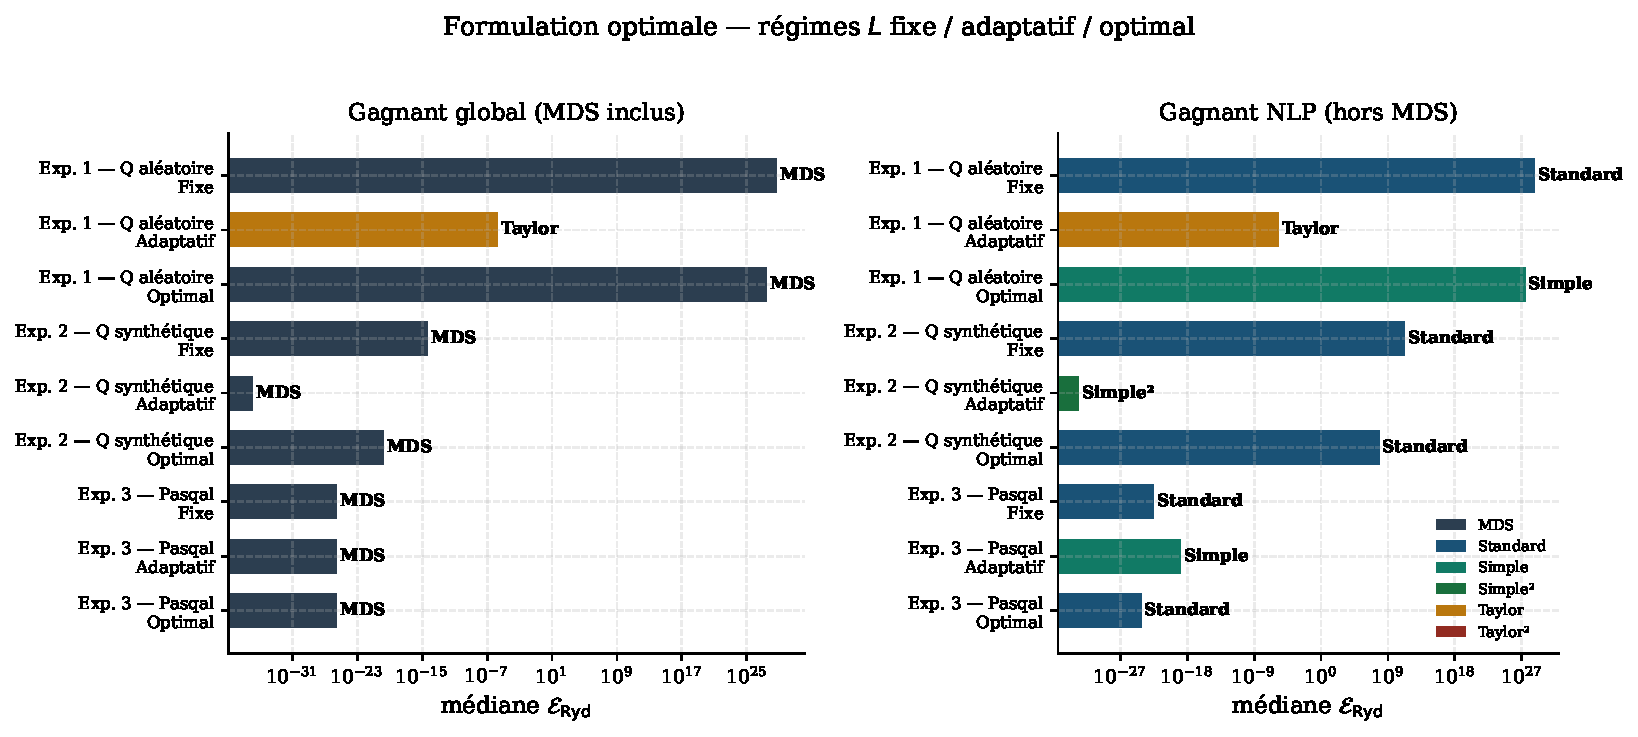
\includegraphics[width=0.95\textwidth]{figures/lregime_winners.pdf}
  \caption{Meilleure formulation selon le régime $L$ (fixe / adaptatif / optimal)
  pour les trois expériences. Gauche : gagnant global (MDS inclus) ;
  droite : meilleur NLP hors MDS.}
  \label{fig:lregime-winners}
\end{figure}

\begin{figure}[H]
  \centering
  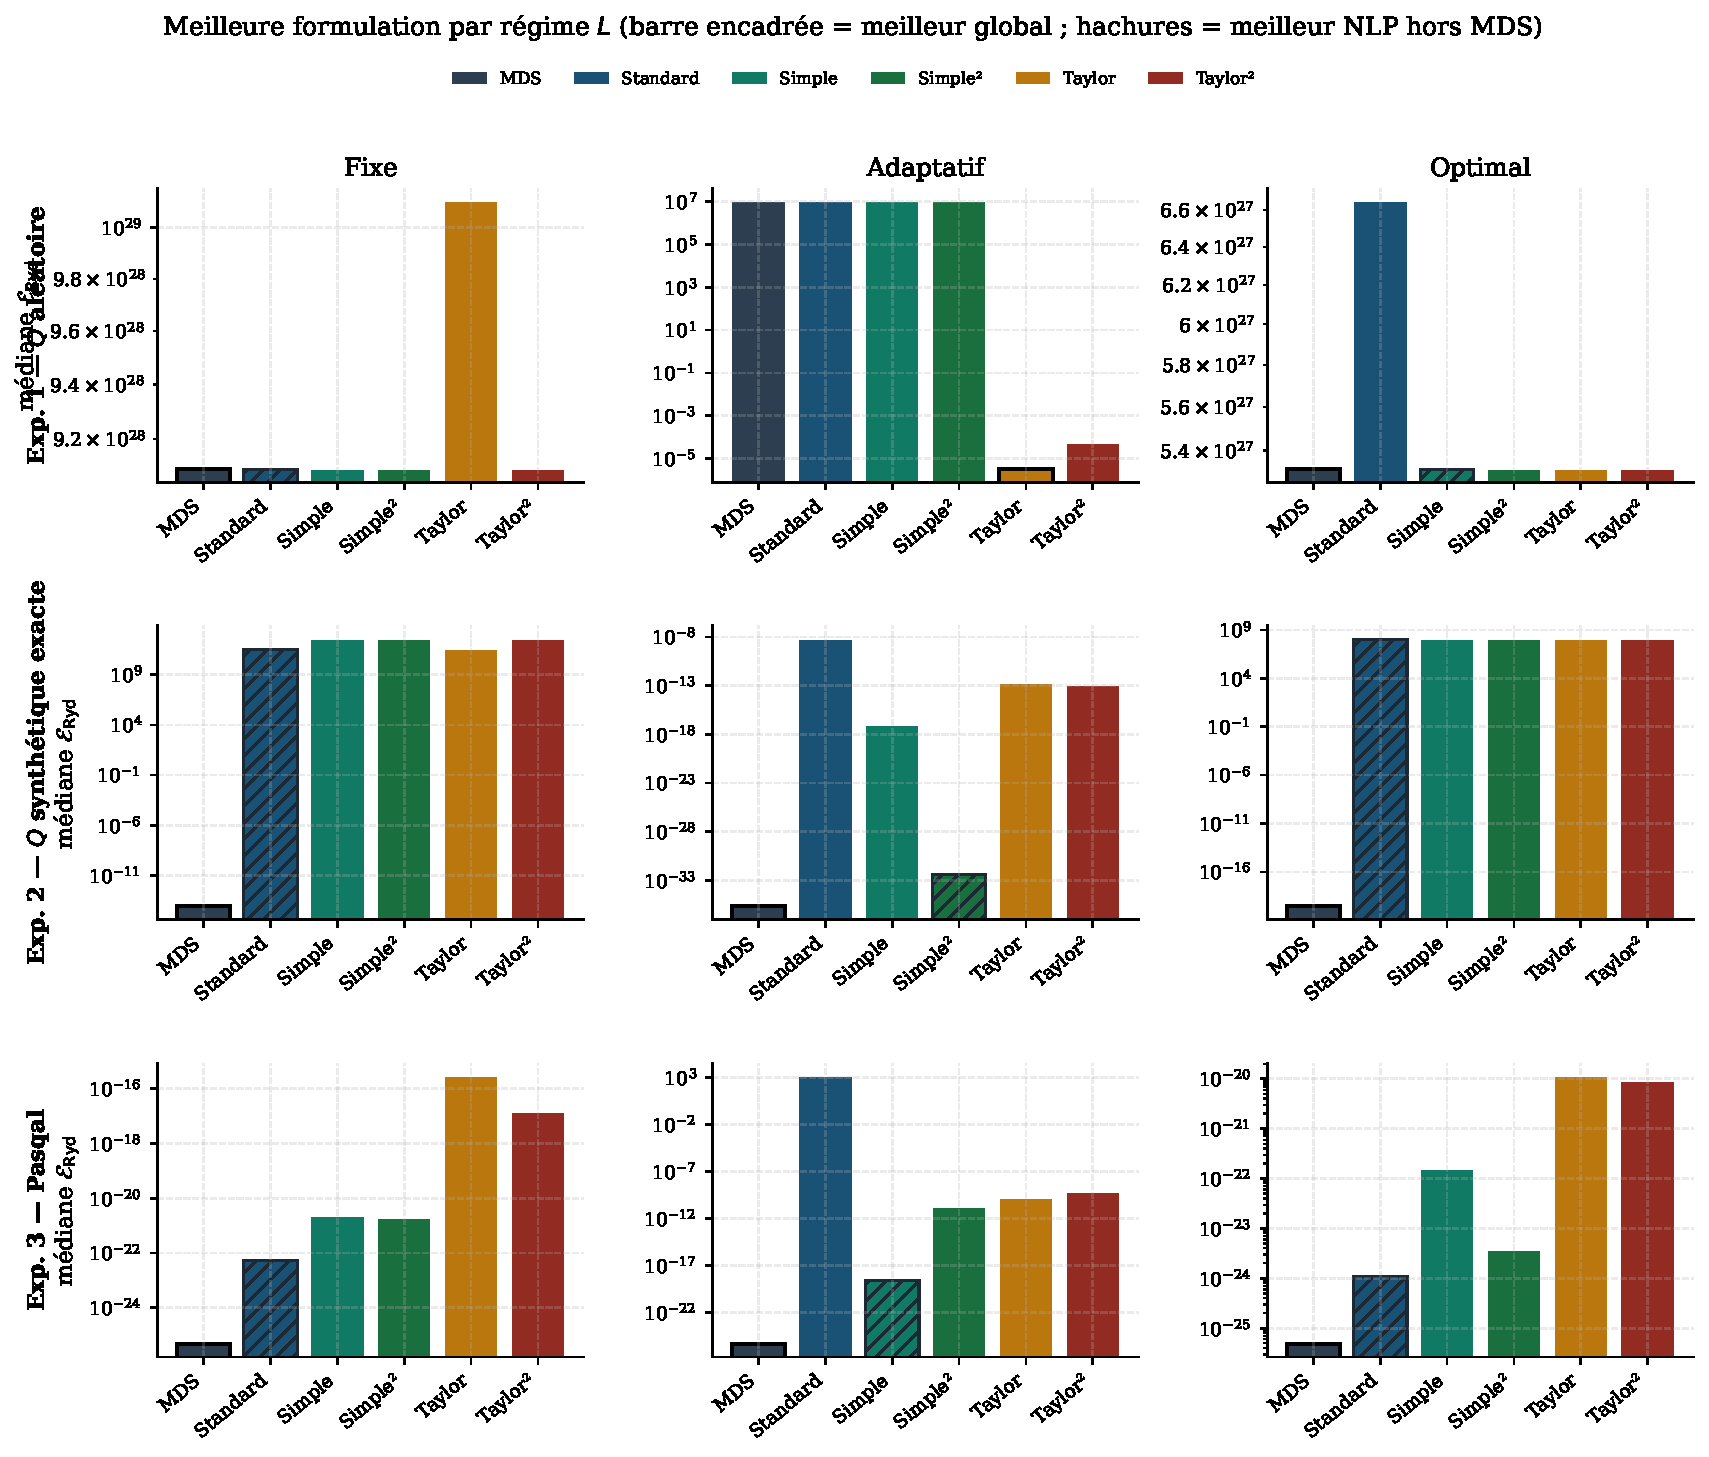
\includegraphics[width=\textwidth]{figures/lregime_bars_3exp.pdf}
  \caption{Comparaison des formulations pour chaque couple
  (expérience $\times$ régime $L$). Barre encadrée = meilleur global ;
  hachures = meilleur NLP hors MDS.}
  \label{fig:lregime-bars}
\end{figure}

\begin{figure}[H]
  \centering
  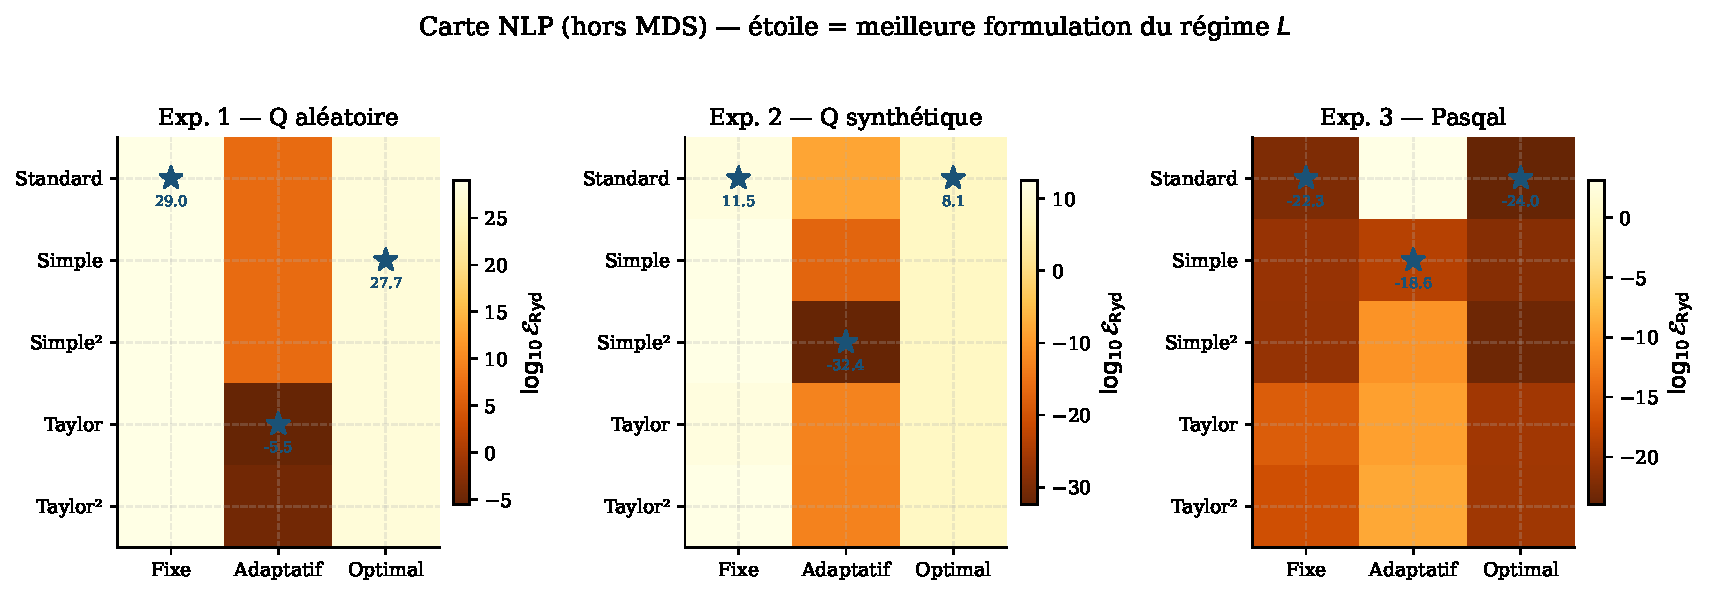
\includegraphics[width=\textwidth]{figures/lregime_nlp_heatmap.pdf}
  \caption{Carte $\log_{10}\Eryd$ des formulations NLP (hors MDS).
  L'étoile marque la meilleure NLP de chaque régime $L$.}
  \label{fig:lregime-heatmap}
\end{figure}

\subsection{Expérience~4 : $L$ variable et $\alpha L$}
\label{sec:res-exp4}

On compare les cinq formulations NLP lorsque $L$ est une variable de décision
et que l'objectif contient la pénalité $\alpha L$, avec ou sans contrainte
$\|x_i-x_j\|\ge z_{\min}^{\mathrm{opt}}$.
Les trois jeux de données de l'expérience~4 sont retenus :
Pasqal, synthétique et aléatoire.
Le tableau~\ref{tab:lalpha-overview} les compare.
Les deux derniers sont maintenant étendus via
\texttt{exp\_L\_alpha\_full\_results\_n4\_50.csv}, qui couvre
$n\in\{4,10,20,30,40,50\}$ pour le synthétique et $n\in\{4,10,20,30,40\}$
pour l'aléatoire.

% Auto-generated — L-variable + α·L overview
\begin{table}[H]
\centering
\caption{Expérience~$L$ variable : pénalité $\alpha L$ et vérification $d_{\min}(\hat{\mathbf{x}}) \approx z_{\min}^{\mathrm{opt}} = (\cSix/Q_{\max})^{1/6}$. Taux de concordance ($|d_{\min}-z_{\min}|/z_{\min}<0{,}2$) et $\mathcal{E}_{\mathrm{Ryd}}$ médiane pour $\alpha=10^{-4}$. Pasqal : 48 fichiers GML, $n=25$ ; synthétique : 5 instances, $n\in\{4,10,20,30,40,50\}$ ; aléatoire : 1 instance, $n\in\{4,10,20,30,40\}$.}
\label{tab:lalpha-overview}
\footnotesize
\setlength{\tabcolsep}{3.5pt}
\renewcommand{\arraystretch}{1.05}
\begin{tabular}{@{}llcccc@{}}
  \toprule
  Source & Formulation & \multicolumn{2}{c}{avec $z_{\min}$} & \multicolumn{2}{c}{sans $z_{\min}$} \\
  \cmidrule(lr){3-4}\cmidrule(lr){5-6}
   &  & Concord. & $\mathcal{E}_{\mathrm{Ryd}}$ & Concord. & $\mathcal{E}_{\mathrm{Ryd}}$ \\
  \midrule
  Pasqal (GML) & Standard & 100\% & $1.18\times10^{-8}$ & 100\% & $\mathbf{4.74\times10^{-12}}$ \\
   & Simple & 100\% & $\mathbf{9.95\times10^{-10}}$ & 100\% & $1.67\times10^{-8}$ \\
   & Simple$^2$ & 100\% & $6.33\times10^{-11}$ & 100\% & $\mathbf{2.34\times10^{-11}}$ \\
   & Taylor & 100\% & $\mathbf{4.26\times10^{-12}}$ & 100\% & $4.74\times10^{-12}$ \\
   & Taylor$^2$ & 100\% & $\mathbf{7.38\times10^{-13}}$ & 100\% & $8.47\times10^{-13}$ \\
  \midrule
  $Q$ exacte synthétique & Standard & 67\% & $9.20\times10^{-3}$ & 87\% & $\mathbf{1.30\times10^{-4}}$ \\
   & Simple & 100\% & $5.05\times10^{-6}$ & 100\% & $\mathbf{4.41\times10^{-7}}$ \\
   & Simple$^2$ & 100\% & $1.92\times10^{-7}$ & 100\% & $\mathbf{3.66\times10^{-12}}$ \\
   & Taylor & 90\% & $\mathbf{7.88\times10^{-1}}$ & 47\% & $2.16\times10^{10}$ \\
   & Taylor$^2$ & 80\% & $\mathbf{5.25\times10^{1}}$ & 67\% & $7.89\times10^{5}$ \\
  \midrule
  $Q$ aléatoire & Standard & 80\% & $5.47\times10^{21}$ & 40\% & $\mathbf{1.32\times10^{1}}$ \\
   & Simple & 20\% & $9.65\times10^{23}$ & 20\% & $\mathbf{9.65\times10^{23}}$ \\
   & Simple$^2$ & 20\% & $\mathbf{9.65\times10^{23}}$ & 20\% & $\mathbf{9.65\times10^{23}}$ \\
   & Taylor & 40\% & $\mathbf{9.65\times10^{23}}$ & 20\% & $4.25\times10^{26}$ \\
   & Taylor$^2$ & 60\% & $\mathbf{1.52\times10^{24}}$ & 40\% & $1.87\times10^{25}$ \\
  \bottomrule
\end{tabular}
\end{table}

% Auto-generated — L-α detail (exp3_pasqal)
\begin{table}[H]
\centering
\caption{Pasqal (GML) (48 fichiers GML, $n=25$) : $L$ variable, objectif $f(\mathbf{x})+\alpha L$. Concordance $d_{\min}\approx z_{\min}^{\mathrm{opt}}$, $\bar L$ et $\mathcal{E}_{\mathrm{Ryd}}$ médiane.}
\label{tab:lalpha-pasqal}
\footnotesize
\setlength{\tabcolsep}{3pt}
\renewcommand{\arraystretch}{1.05}
\begin{tabular}{@{}llrrcrrc@{}}
  \toprule
  Form. & $\alpha$ & \multicolumn{3}{c}{avec $z_{\min}$} & \multicolumn{3}{c}{sans $z_{\min}$} \\
  \cmidrule(lr){3-5}\cmidrule(lr){6-8}
   &  & Conc. & $\bar L$ & $\mathcal{E}_{\mathrm{Ryd}}$ & Conc. & $\bar L$ & $\mathcal{E}_{\mathrm{Ryd}}$ \\
  \midrule
  Standard & $10^{-6}$ & 77\% & 3153 & $2.77\times10^{-13}$ & 100\% & 4.50 & $5.80\times10^{-15}$ \\
   & $10^{-4}$ & 100\% & 4.48 & $1.18\times10^{-8}$ & 100\% & 4.21 & $4.74\times10^{-12}$ \\
   & $10^{-2}$ & 100\% & 4.20 & $4.25\times10^{-8}$ & 100\% & 4.20 & $4.48\times10^{-8}$ \\
   & $1$ & 100\% & 4.05 & $4.24\times10^{-4}$ & 100\% & 4.05 & $4.48\times10^{-4}$ \\
  \midrule
  Simple & $10^{-6}$ & 100\% & 4.21 & $7.84\times10^{-10}$ & 100\% & 8.42 & $1.67\times10^{-12}$ \\
   & $10^{-4}$ & 100\% & 4.21 & $9.95\times10^{-10}$ & 100\% & 4.29 & $1.67\times10^{-8}$ \\
   & $10^{-2}$ & 100\% & 4.21 & $5.75\times10^{-6}$ & 100\% & 4.26 & $1.67\times10^{-4}$ \\
   & $1$ & 100\% & 4.19 & $5.97\times10^{-2}$ & 100\% & 4.21 & $1.86\times10^{0}$ \\
  \midrule
  Simple$^2$ & $10^{-6}$ & 100\% & 4.21 & $9.57\times10^{-11}$ & 100\% & 4.21 & $2.56\times10^{-15}$ \\
   & $10^{-4}$ & 100\% & 4.48 & $6.33\times10^{-11}$ & 100\% & 4.29 & $2.34\times10^{-11}$ \\
   & $10^{-2}$ & 100\% & 4.48 & $3.12\times10^{-8}$ & 100\% & 4.26 & $2.31\times10^{-7}$ \\
   & $1$ & 100\% & 4.21 & $2.13\times10^{-5}$ & 100\% & 4.26 & $2.31\times10^{-3}$ \\
  \midrule
  Taylor & $10^{-6}$ & 100\% & 4.21 & $6.58\times10^{-13}$ & 100\% & 4.21 & $5.80\times10^{-15}$ \\
   & $10^{-4}$ & 100\% & 4.21 & $4.26\times10^{-12}$ & 100\% & 4.46 & $4.74\times10^{-12}$ \\
   & $10^{-2}$ & 100\% & 4.20 & $4.25\times10^{-8}$ & 100\% & 4.20 & $4.48\times10^{-8}$ \\
   & $1$ & 100\% & 3.80 & $4.26\times10^{-4}$ & 67\% & 3.50 & $4.50\times10^{-4}$ \\
  \midrule
  Taylor$^2$ & $10^{-6}$ & 100\% & 4.21 & $7.69\times10^{-14}$ & 100\% & 4.21 & $2.75\times10^{-16}$ \\
   & $10^{-4}$ & 100\% & 4.21 & $7.38\times10^{-13}$ & 100\% & 4.48 & $8.47\times10^{-13}$ \\
   & $10^{-2}$ & 100\% & 4.21 & $7.36\times10^{-9}$ & 100\% & 4.21 & $8.54\times10^{-9}$ \\
   & $1$ & 100\% & 4.12 & $7.37\times10^{-5}$ & 100\% & 4.12 & $8.52\times10^{-5}$ \\
  \bottomrule
\end{tabular}
\end{table}

% Auto-generated — L-α detail (exp2_Q_exacte_synthetique)
\begin{table}[H]
\centering
\caption{$Q$ exacte synthétique (5 instances, $n\in\{4,10,20,30,40,50\}$) : $L$ variable, objectif $f(\mathbf{x})+\alpha L$. Concordance $d_{\min}\approx z_{\min}^{\mathrm{opt}}$, $\bar L$ et $\mathcal{E}_{\mathrm{Ryd}}$ médiane.}
\label{tab:lalpha-synth}
\footnotesize
\setlength{\tabcolsep}{3pt}
\renewcommand{\arraystretch}{1.05}
\begin{tabular}{@{}llrrcrrc@{}}
  \toprule
  Form. & $\alpha$ & \multicolumn{3}{c}{avec $z_{\min}$} & \multicolumn{3}{c}{sans $z_{\min}$} \\
  \cmidrule(lr){3-5}\cmidrule(lr){6-8}
   &  & Conc. & $\bar L$ & $\mathcal{E}_{\mathrm{Ryd}}$ & Conc. & $\bar L$ & $\mathcal{E}_{\mathrm{Ryd}}$ \\
  \midrule
  Standard & $10^{-6}$ & 63\% & 236 & $2.35\times10^{-2}$ & 90\% & 147 & $2.37\times10^{-4}$ \\
   & $10^{-4}$ & 67\% & 6722 & $9.20\times10^{-3}$ & 87\% & 49.0 & $1.30\times10^{-4}$ \\
   & $10^{-2}$ & 77\% & 525 & $6.65\times10^{-3}$ & 87\% & 17.4 & $3.46\times10^{-3}$ \\
   & $1$ & 60\% & 158 & $3.16\times10^{-1}$ & 80\% & 6.86 & $3.12\times10^{-1}$ \\
  \midrule
  Simple & $10^{-6}$ & 100\% & 9.05 & $6.92\times10^{-6}$ & 100\% & 11.1 & $1.97\times10^{-12}$ \\
   & $10^{-4}$ & 100\% & 9.07 & $5.05\times10^{-6}$ & 100\% & 8.96 & $4.41\times10^{-7}$ \\
   & $10^{-2}$ & 100\% & 9.04 & $3.02\times10^{-4}$ & 100\% & 9.03 & $4.22\times10^{-3}$ \\
   & $1$ & 100\% & 8.83 & $3.11\times10^{0}$ & 97\% & 8.80 & $4.44\times10^{1}$ \\
  \midrule
  Simple$^2$ & $10^{-6}$ & 97\% & 142 & $4.17\times10^{-7}$ & 100\% & 15.9 & $1.30\times10^{-15}$ \\
   & $10^{-4}$ & 100\% & 8.98 & $1.92\times10^{-7}$ & 100\% & 8.99 & $3.66\times10^{-12}$ \\
   & $10^{-2}$ & 100\% & 8.97 & $6.04\times10^{-7}$ & 100\% & 8.97 & $2.59\times10^{-8}$ \\
   & $1$ & 100\% & 8.91 & $2.61\times10^{-4}$ & 100\% & 8.97 & $2.55\times10^{-3}$ \\
  \midrule
  Taylor & $10^{-6}$ & 93\% & 6104 & $9.82\times10^{-2}$ & 60\% & 64589 & $1.08\times10^{2}$ \\
   & $10^{-4}$ & 90\% & 162 & $7.88\times10^{-1}$ & 47\% & 57190 & $2.16\times10^{10}$ \\
   & $10^{-2}$ & 93\% & 4330 & $1.33\times10^{0}$ & 27\% & 60605 & $3.44\times10^{12}$ \\
   & $1$ & 90\% & 8.00 & $1.53\times10^{4}$ & 3\% & 4942 & $1.02\times10^{37}$ \\
  \midrule
  Taylor$^2$ & $10^{-6}$ & 87\% & 81289 & $1.55\times10^{0}$ & 87\% & 84704 & $1.88\times10^{5}$ \\
   & $10^{-4}$ & 80\% & 61399 & $5.25\times10^{1}$ & 67\% & 79481 & $7.89\times10^{5}$ \\
   & $10^{-2}$ & 73\% & 72824 & $1.10\times10^{5}$ & 37\% & 62066 & $5.47\times10^{9}$ \\
   & $1$ & 80\% & 35768 & $7.23\times10^{6}$ & 7\% & 28482 & $7.34\times10^{29}$ \\
  \bottomrule
\end{tabular}
\end{table}

% Auto-generated — L-α detail (exp1_Q_aleatoire)
\begin{table}[H]
\centering
\caption{$Q$ aléatoire (1 instance, $n\in\{4,10,20,30,40\}$) : $L$ variable, objectif $f(\mathbf{x})+\alpha L$. Concordance $d_{\min}\approx z_{\min}^{\mathrm{opt}}$, $\bar L$ et $\mathcal{E}_{\mathrm{Ryd}}$ médiane.}
\label{tab:lalpha-rand}
\footnotesize
\setlength{\tabcolsep}{3pt}
\renewcommand{\arraystretch}{1.05}
\begin{tabular}{@{}llrrcrrc@{}}
  \toprule
  Form. & $\alpha$ & \multicolumn{3}{c}{avec $z_{\min}$} & \multicolumn{3}{c}{sans $z_{\min}$} \\
  \cmidrule(lr){3-5}\cmidrule(lr){6-8}
   &  & Conc. & $\bar L$ & $\mathcal{E}_{\mathrm{Ryd}}$ & Conc. & $\bar L$ & $\mathcal{E}_{\mathrm{Ryd}}$ \\
  \midrule
  Standard & $10^{-6}$ & 80\% & 159 & $5.47\times10^{21}$ & 60\% & 1059 & $2.64\times10^{1}$ \\
   & $10^{-4}$ & 80\% & 106 & $5.47\times10^{21}$ & 40\% & 29.6 & $1.32\times10^{1}$ \\
   & $10^{-2}$ & 100\% & 83.1 & $5.35\times10^{12}$ & 20\% & 2.73 & $1.32\times10^{1}$ \\
   & $1$ & 100\% & 154 & $5.35\times10^{12}$ & 20\% & 3.08 & $2.95\times10^{1}$ \\
  \midrule
  Simple & $10^{-6}$ & 20\% & 7.55 & $9.65\times10^{23}$ & 20\% & 7.97 & $9.65\times10^{23}$ \\
   & $10^{-4}$ & 20\% & 7.60 & $9.65\times10^{23}$ & 20\% & 7.69 & $9.65\times10^{23}$ \\
   & $10^{-2}$ & 20\% & 7.60 & $9.65\times10^{23}$ & 20\% & 7.68 & $9.65\times10^{23}$ \\
   & $1$ & 20\% & 7.43 & $9.65\times10^{23}$ & 20\% & 7.42 & $9.65\times10^{23}$ \\
  \midrule
  Simple$^2$ & $10^{-6}$ & 20\% & 3111 & $9.65\times10^{23}$ & 20\% & 38.3 & $9.65\times10^{23}$ \\
   & $10^{-4}$ & 20\% & 7.75 & $9.65\times10^{23}$ & 20\% & 7.75 & $9.65\times10^{23}$ \\
   & $10^{-2}$ & 20\% & 7.82 & $9.65\times10^{23}$ & 20\% & 7.72 & $9.65\times10^{23}$ \\
   & $1$ & 20\% & 7.65 & $9.65\times10^{23}$ & 20\% & 7.75 & $9.65\times10^{23}$ \\
  \midrule
  Taylor & $10^{-6}$ & 60\% & 60570 & $2.16\times10^{20}$ & 40\% & 148849 & $1.02\times10^{23}$ \\
   & $10^{-4}$ & 40\% & 29958 & $9.65\times10^{23}$ & 20\% & 147232 & $4.25\times10^{26}$ \\
   & $10^{-2}$ & 40\% & 15930 & $9.65\times10^{23}$ & 20\% & 139758 & $1.92\times10^{25}$ \\
   & $1$ & 40\% & 23406 & $9.65\times10^{23}$ & 0\% & 130355 & $8.29\times10^{26}$ \\
  \midrule
  Taylor$^2$ & $10^{-6}$ & 60\% & 319342 & $5.49\times10^{23}$ & 60\% & 153963 & $8.66\times10^{22}$ \\
   & $10^{-4}$ & 60\% & 134680 & $1.52\times10^{24}$ & 40\% & 145025 & $1.87\times10^{25}$ \\
   & $10^{-2}$ & 60\% & 140532 & $1.27\times10^{22}$ & 40\% & 116791 & $1.94\times10^{25}$ \\
   & $1$ & 60\% & 137872 & $5.53\times10^{20}$ & 20\% & 118916 & $8.74\times10^{26}$ \\
  \bottomrule
\end{tabular}
\end{table}


\paragraph{Quelle formulation est la meilleure ?}
Les figures~\ref{fig:lalpha-winners}--\ref{fig:lalpha-alpha}
résument, sur les trois jeux de données, le classement des formulations.
\begin{itemize}[leftmargin=*, itemsep=2pt]
  \item \textbf{Pasqal ($\alpha L$, $n=25$, 48~GML).}
    Toutes les formulations atteignent $100\%$ de concordance pour
    $\alpha\le 10^{-2}$. En erreur Rydberg, Taylor$^2$ (puis
    Simple$^2$ / Taylor) est le plus précis sur ces graphes sparses.
  \item \textbf{Synthétique.} L'extension $n\le 50$ confirme la même hiérarchie
    globale pour les petites pénalités : Simple$^2$ et Taylor$^2$ dominent
    quand la contrainte $z_{\min}$ est active, tandis que Taylor peut devenir
    instable sans cette contrainte quand $\alpha$ augmente.
  \item \textbf{Aléatoire.} Les runs étendus montrent une dispersion plus forte,
    mais le diagnostic reste le même : les formulations quadratiques sont
    plus robustes, alors que les variantes Taylor sans $z_{\min}$ peuvent
    se dégrader nettement sur certaines valeurs de $\alpha$.
\end{itemize}

\begin{figure}[H]
  \centering
  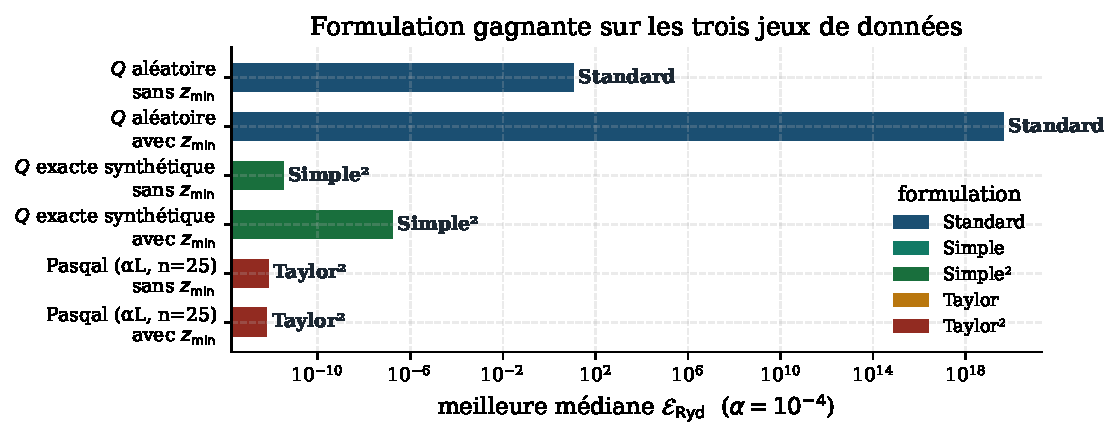
\includegraphics[width=0.92\textwidth]{figures/lalpha_winners.pdf}
  \caption{Formulation minimisant la médiane de $\Eryd$ pour
  $\alpha=10^{-4}$ sur Pasqal, synthétique et aléatoire, avec et sans
  $z_{\min}$.
  Données retenues ici : \texttt{exp\_L\_alpha\_full\_results.csv} pour Pasqal,
  et \texttt{exp\_L\_alpha\_full\_results\_n4\_50.csv} pour les deux autres
  jeux de données.}
  \label{fig:lalpha-winners}
\end{figure}

\begin{figure}[H]
  \centering
  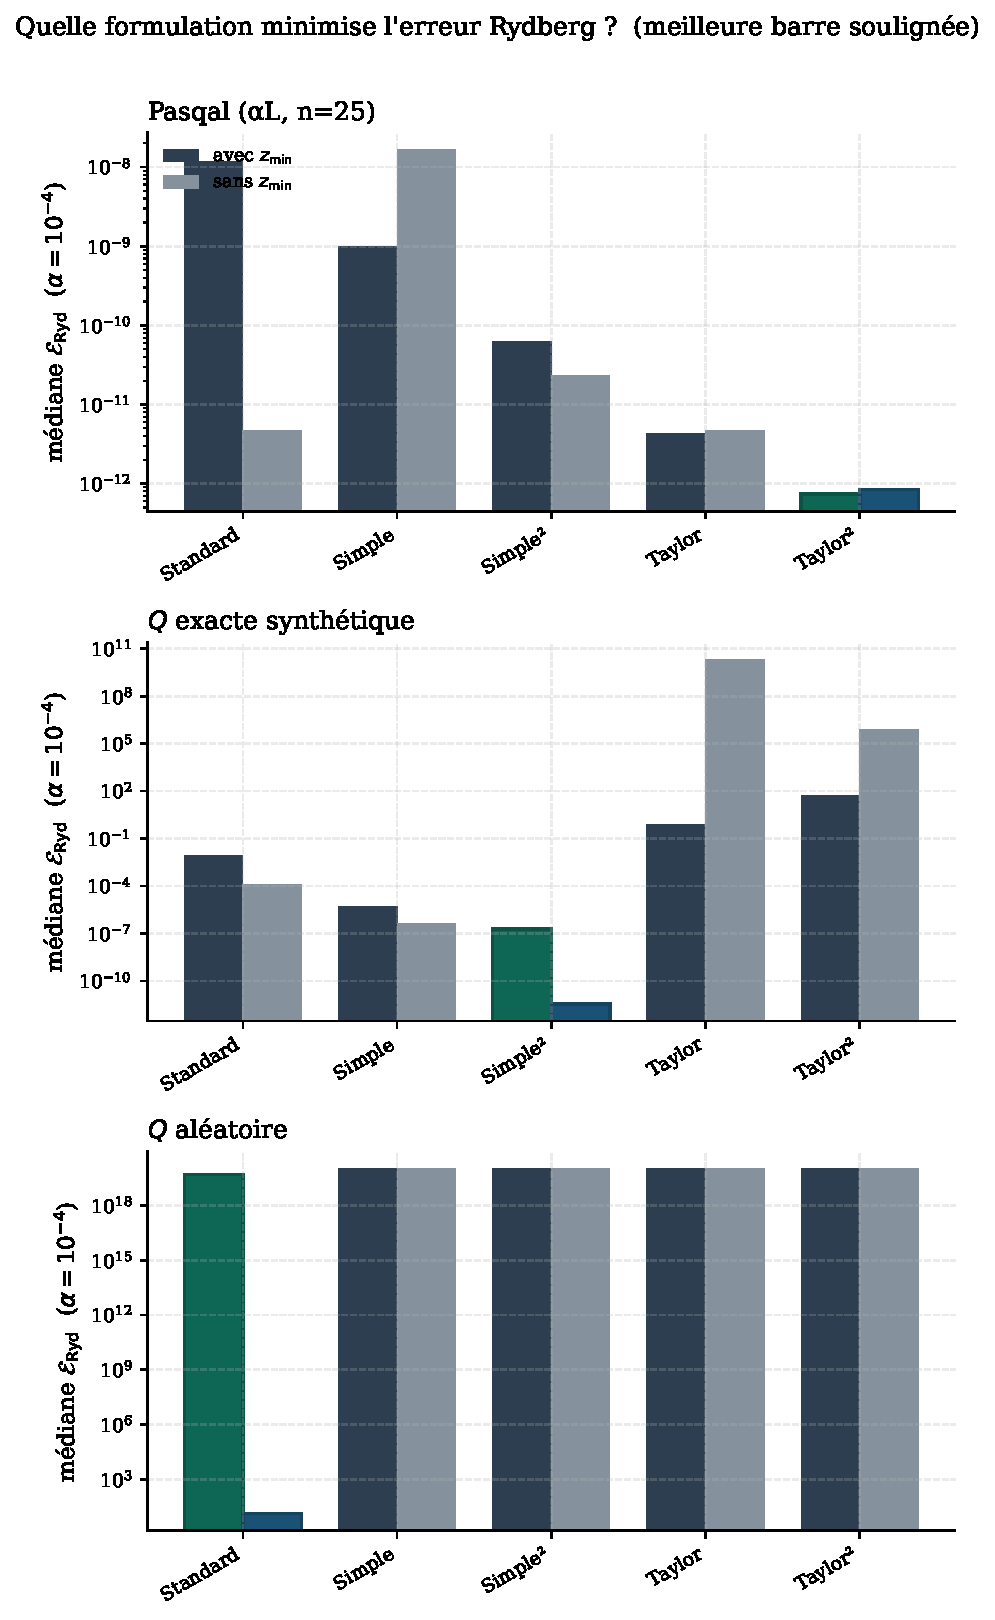
\includegraphics[width=\textwidth]{figures/lalpha_best_err_by_source.pdf}
  \caption{Médiane de $\Eryd$ par formulation sur Pasqal ($\alpha=10^{-4}$).
  Barres foncées : avec $z_{\min}$ ; barres claires : sans $z_{\min}$.
  La meilleure barre de chaque groupe est soulignée.
  Les trois panneaux correspondent à Pasqal, synthétique et aléatoire.}
  \label{fig:lalpha-best-err}
\end{figure}

\begin{figure}[H]
  \centering
  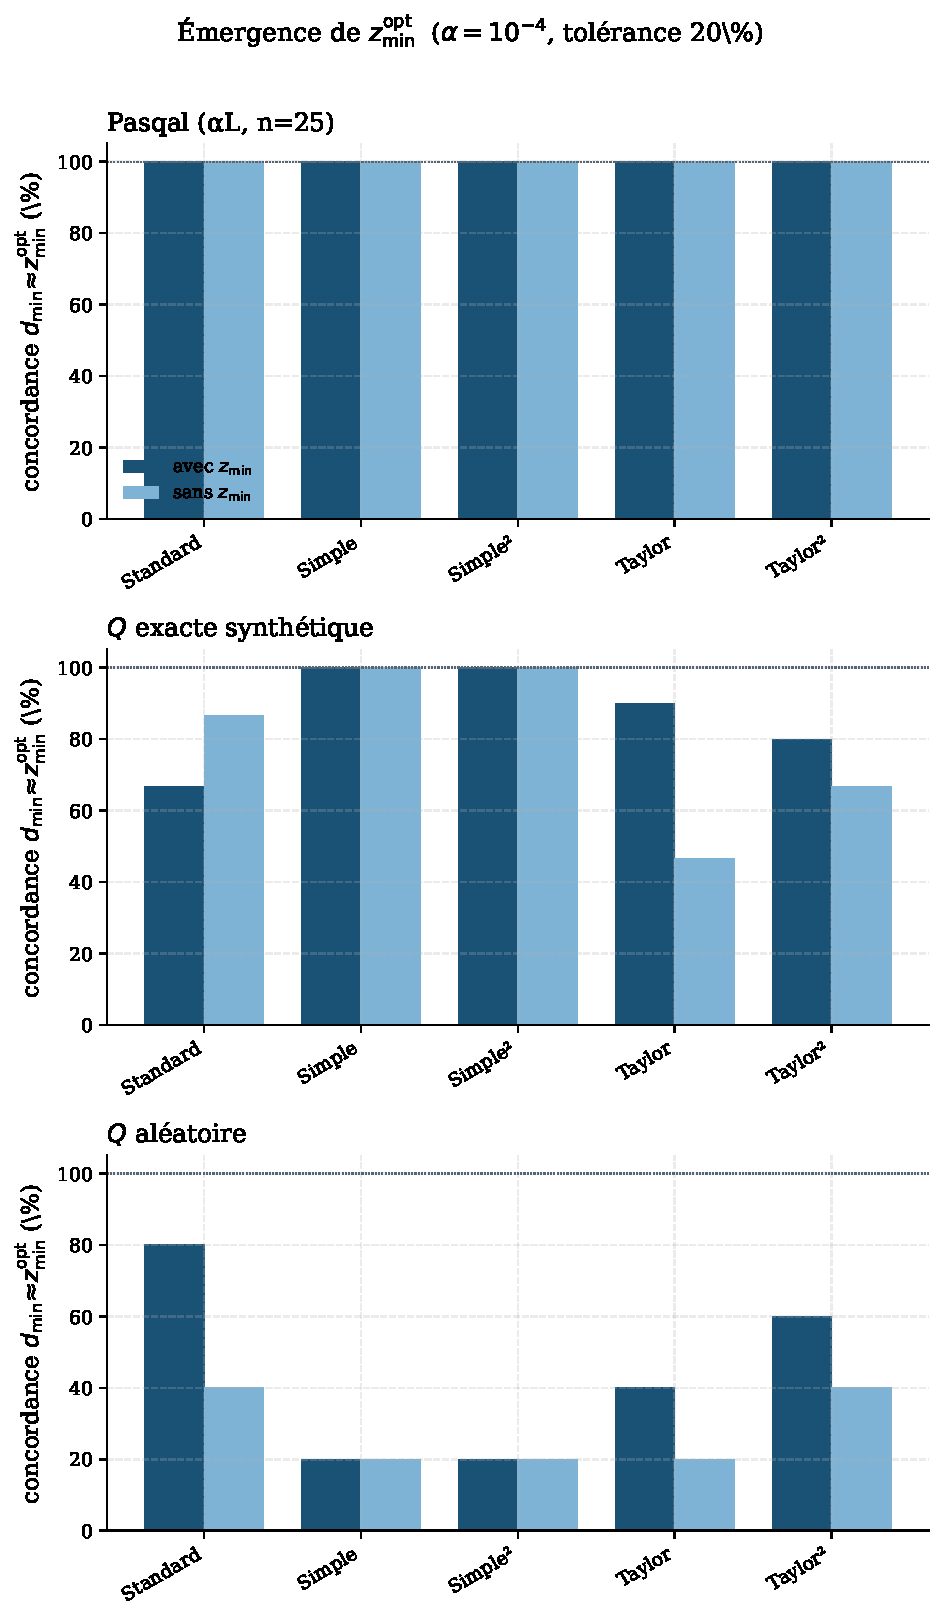
\includegraphics[width=\textwidth]{figures/lalpha_match_by_source.pdf}
  \caption{Taux de concordance
  $d_{\min}\approx z_{\min}^{\mathrm{opt}}$
  ($|d_{\min}-z_{\min}|/z_{\min}<0{,}2$) sur Pasqal, synthétique et aléatoire,
  pour $\alpha=10^{-4}$.}
  \label{fig:lalpha-match}
\end{figure}

\begin{figure}[H]
  \centering
  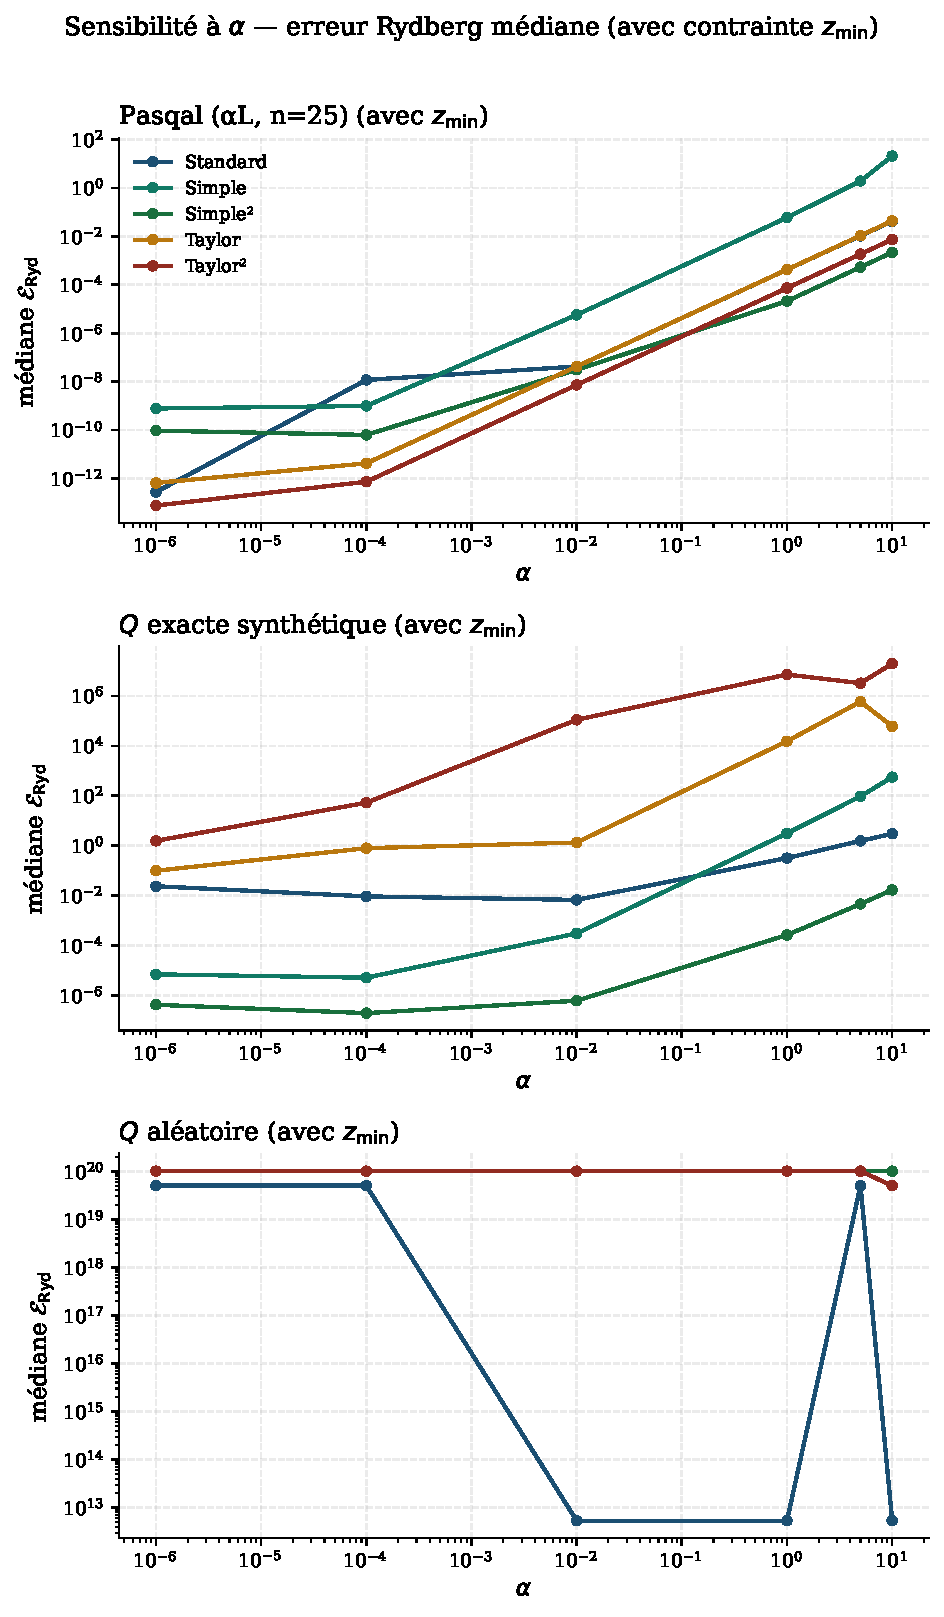
\includegraphics[width=\textwidth]{figures/lalpha_err_vs_alpha.pdf}
  \caption{Sensibilité à $\alpha$ : médiane de $\Eryd$ (échelle log)
  avec contrainte $z_{\min}$, sur Pasqal, synthétique et aléatoire.}
  \label{fig:lalpha-alpha}
\end{figure}

\paragraph{Observations complémentaires.}
(i)~\textbf{Pasqal.} Pour $\alpha\le 10^{-2}$, toutes les formulations
atteignent $100\%$ de concordance $d_{\min}\approx z_{\min}^{\mathrm{opt}}$
(avec \emph{et} sans contrainte $z_{\min}$), avec $\Eryd$ médiane souvent
sous $10^{-10}$ pour $\alpha=10^{-4}$.
(ii)~\textbf{Synthétique.} Les formules quadratiques restent les plus régulières
sur $n\le 50$ et la contrainte $z_{\min}$ continue de stabiliser les variantes
Taylor quand $\alpha$ augmente.
(iii)~\textbf{Aléatoire.} Le run étendu renforce le contraste entre
les formulations robustes et celles qui divergent sans contrainte,
en particulier sur les plus grandes valeurs de $\alpha$.

\section{Discussion}
\label{sec:discussion}

\paragraph{MDS vs NLP.}
Sur données exactes, le MDS exact est imbattable en précision et en temps :
il exploite directement la structure euclidienne induite par~\eqref{eq:D2}.
Les NLP deviennent indispensables lorsque des contraintes expérimentales
(bornes, topologie sparse type instances Pasqal) brisent l'hypothèse MDS.

\paragraph{Dissociation $\Eryd$ / RMSE.}
Un $L$ trop grand ($L = 100\sqrt{n}$) produit des $\Eryd$ infinitésimales
mais des RMSE de l'ordre de $10^2$ (expérience~1, $n=4$, $L$ adaptatif) : le solveur
«~étire~» la configuration pour annihiler les termes $1/r_{ij}^6$ sans
reproduire la géométrie de référence. \texttt{L\_optimal}, calibré sur
$r_{\min}$, améliore le RMSE mais peut dégrader certaines NLP.

\paragraph{Taylor vs Simple.}
Taylor (et Taylor$^2$) excellent lorsque $Q$ est proche d'une réalisation
euclidienne et que l'initialisation est près de $d_{ij}$ ; Simple et
Simple$^2$ sont plus robustes sur les graphes Pasqal sparses et en régime
$L$ adaptatif.

\paragraph{$L$ variable et $\alpha L$.}
Traiter $L$ comme variable avec pénalité $\alpha L$ et
$z_{\min}^{\mathrm{opt}}=(\cSix/Q_{\max})^{1/6}$ permet de découvrir
l'échelle sans la fixer a priori.
Sur $Q$ exacte synthétique, Simple$^2$ (puis Simple) est le meilleur
choix ; sur Pasqal, Taylor$^2$ / Simple$^2$ ; sur $Q$ aléatoire, Standard.
Un $\alpha$ petit ($10^{-6}$--$10^{-4}$) conserve une $\Eryd$ faible tout
en reproduisant $z_{\min}^{\mathrm{opt}}$ \emph{même sans} imposer la
contrainte de distance (surtout Simple / Simple$^2$ sur données exactes).
Taylor sans $z_{\min}$ est fragile (poids $36\,Q^{7/3}$).
Le scaling cohérent~\eqref{eq:scaling-coherent} remet ensuite
la solution dans une boîte $L_{\mathrm{choisi}}$ sans casser le modèle
Rydberg ($Q'=Q/\lambda^6$).
Voir figures~\ref{fig:lalpha-winners}--\ref{fig:lalpha-alpha}.

\paragraph{Perspectives.}
(i)~Normaliser les coordonnées dans $[0,1]^d$ avant optimisation puis
remonter à l'échelle physique~\cite{henry2024}.
(ii)~Coupler MDS (initialisation) + raffinement NLP contraint.
(iii)~Calibrer $\alpha$ automatiquement (par ex.\ continuation) et étendre
le protocole $L$ variable à $n$ plus grands.
(iv)~Extension $d=3$ et prise en compte de la décroissance $1/r^3$ dipolaire.

\section{Conclusion}
\label{sec:conclusion}

Nous avons formalisé et benchmarké le problème inverse de reconstruction
de positions d'atomes de Rydberg à partir d'interactions van der Waals.
Six formulations couvrent le spectre direct (Standard), lifté (Simple,
Simple$^2$), approximé (Taylor, Taylor$^2$) et algébrique (MDS). Deux métriques
--- $\Eryd$ et RMSE --- sont nécessaires pour
évaluer respectivement la cohérence physique et la fidélité géométrique.
Le MDS spectral avec projection PSD domine sur données exactes ; le choix
de $L$ est aussi déterminant que le choix de formulation. En traitant $L$
comme variable avec pénalité $\alpha L$ et
$z_{\min}^{\mathrm{opt}}=(\cSix/Q_{\max})^{1/6}$, on retrouve sur Pasqal
et $Q$ exacte une échelle cohérente et, pour Simple / Simple$^2$, la
distance minimale optimale même sans contrainte explicite. Les travaux futurs
porteront sur le calibrage de $\alpha$ et l'hybridation MDS--NLP pour
données bruitées et contraintes expérimentales.

\paragraph{Pipeline.}
\[
  \underbrace{Q}_{\text{mesures}}
  \;\xrightarrow{\;\text{NLP ou MDS}\;}
  \underbrace{\hat{\mathbf{x}}}_{\text{positions}}
  \;\xrightarrow{\;\Eryd,\,\mathrm{RMSE}\;}
  \underbrace{\text{évaluation}}_{\text{benchmark}}.
\]

%\appendix
%% Auto-generated — Exp. 1 full summary tables
\section{Résultats détaillés --- Expérience~1 ($Q_{\mathrm{bruit\,dist}}$)}
\label{app:exp1}

Matrice $Q$ générée aléatoirement via \texttt{Q\_bruit\_dist} ; objectif : retrouver $\mathbf{x}$ minimisant $\mathcal{E}_{\mathrm{Ryd}}$. Moyennes sur 10 instances indépendantes.

\subsection{$n=4$, Fixe ($L{=}10$)}
\begin{table}[H]
\centering
\small
\begin{tabular}{@{}lrr@{}}
  \toprule
  Formulation & $\mathcal{E}_{\mathrm{Ryd}}$ & Temps moy. \\
  \midrule
  MDS exact & $6.79\times10^{10}$ & 0.24\,s \\
  Standard & $7.23\times10^{10}$ & 1.0\,s \\
  Taylor & $\mathbf{6.51\times10^{10}}$ & 0.28\,s \\
  Taylor$^2$ & $6.51\times10^{10}$ & 0.42\,s \\
  Simple$^2$ & $6.79\times10^{10}$ & 0.13\,s \\
  Simple & $6.79\times10^{10}$ & 0.13\,s \\
  \bottomrule
\end{tabular}
\end{table}

\subsection{$n=4$, Adaptatif ($L{=}100\sqrt{n}$)}
\begin{table}[H]
\centering
\small
\begin{tabular}{@{}lrr@{}}
  \toprule
  Formulation & $\mathcal{E}_{\mathrm{Ryd}}$ & Temps moy. \\
  \midrule
  MDS exact & $1.30\times10^{-11}$ & 0\,ms \\
  Standard & $1.30\times10^{-11}$ & 0.01\,s \\
  Taylor & $2.56\times10^{-14}$ & 0.01\,s \\
  Taylor$^2$ & $\mathbf{1.67\times10^{-15}}$ & 0.62\,s \\
  Simple$^2$ & $1.69\times10^{-11}$ & 0.09\,s \\
  Simple & $1.30\times10^{-11}$ & 0.04\,s \\
  \bottomrule
\end{tabular}
\end{table}

\subsection{$n=4$, Optimal ($L{\approx}r_{\min}$)}
\begin{table}[H]
\centering
\small
\begin{tabular}{@{}lrr@{}}
  \toprule
  Formulation & $\mathcal{E}_{\mathrm{Ryd}}$ & Temps moy. \\
  \midrule
  MDS exact & $4.42\times10^{8}$ & 0\,ms \\
  Standard & $\mathbf{2.06\times10^{8}}$ & 0.19\,s \\
  Taylor & $2.06\times10^{8}$ & 1.4\,s \\
  Taylor$^2$ & $2.06\times10^{8}$ & 3.3\,s \\
  Simple$^2$ & $4.42\times10^{8}$ & 0.50\,s \\
  Simple & $4.42\times10^{8}$ & 0.05\,s \\
  \bottomrule
\end{tabular}
\end{table}

\subsection{$n=10$, Fixe ($L{=}10$)}
\begin{table}[H]
\centering
\small
\begin{tabular}{@{}lrr@{}}
  \toprule
  Formulation & $\mathcal{E}_{\mathrm{Ryd}}$ & Temps moy. \\
  \midrule
  MDS exact & $\mathbf{7.51\times10^{29}}$ & 0\,ms \\
  Standard & $7.51\times10^{29}$ & 4.3\,s \\
  Taylor & $7.51\times10^{29}$ & 9.3\,s \\
  Taylor$^2$ & $7.51\times10^{29}$ & 7.7\,s \\
  Simple$^2$ & $7.51\times10^{29}$ & 0.24\,s \\
  Simple & $7.51\times10^{29}$ & 0.22\,s \\
  \bottomrule
\end{tabular}
\end{table}

\subsection{$n=10$, Adaptatif ($L{=}100\sqrt{n}$)}
\begin{table}[H]
\centering
\small
\begin{tabular}{@{}lrr@{}}
  \toprule
  Formulation & $\mathcal{E}_{\mathrm{Ryd}}$ & Temps moy. \\
  \midrule
  MDS exact & $9.86\times10^{6}$ & 0\,ms \\
  Standard & $9.86\times10^{6}$ & 0.15\,s \\
  Taylor & $\mathbf{8.15\times10^{-10}}$ & 2.0\,s \\
  Taylor$^2$ & $1.07\times10^{-9}$ & 3.4\,s \\
  Simple$^2$ & $9.86\times10^{6}$ & 0.65\,s \\
  Simple & $9.86\times10^{6}$ & 0.34\,s \\
  \bottomrule
\end{tabular}
\end{table}

\subsection{$n=10$, Optimal ($L{\approx}r_{\min}$)}
\begin{table}[H]
\centering
\small
\begin{tabular}{@{}lrr@{}}
  \toprule
  Formulation & $\mathcal{E}_{\mathrm{Ryd}}$ & Temps moy. \\
  \midrule
  MDS exact & $3.49\times10^{14}$ & 0\,ms \\
  Standard & $3.87\times10^{14}$ & 3.9\,s \\
  Taylor & $\mathbf{3.48\times10^{14}}$ & 4.4\,s \\
  Taylor$^2$ & $3.48\times10^{14}$ & 5.7\,s \\
  Simple$^2$ & $3.49\times10^{14}$ & 0.22\,s \\
  Simple & $3.49\times10^{14}$ & 0.20\,s \\
  \bottomrule
\end{tabular}
\end{table}

\subsection{$n=20$, Fixe ($L{=}10$)}
\begin{table}[H]
\centering
\small
\begin{tabular}{@{}lrr@{}}
  \toprule
  Formulation & $\mathcal{E}_{\mathrm{Ryd}}$ & Temps moy. \\
  \midrule
  MDS exact & $\mathbf{2.66\times10^{26}}$ & 0\,ms \\
  Standard & $2.66\times10^{26}$ & 15.8\,s \\
  Taylor & $2.66\times10^{26}$ & 39.4\,s \\
  Taylor$^2$ & $2.66\times10^{26}$ & 26.1\,s \\
  Simple$^2$ & $2.66\times10^{26}$ & 0.80\,s \\
  Simple & $2.66\times10^{26}$ & 0.72\,s \\
  \bottomrule
\end{tabular}
\end{table}

\subsection{$n=20$, Adaptatif ($L{=}100\sqrt{n}$)}
\begin{table}[H]
\centering
\small
\begin{tabular}{@{}lrr@{}}
  \toprule
  Formulation & $\mathcal{E}_{\mathrm{Ryd}}$ & Temps moy. \\
  \midrule
  MDS exact & $3.26\times10^{6}$ & 1\,ms \\
  Standard & $3.26\times10^{6}$ & 0.15\,s \\
  Taylor & $\mathbf{3.23\times10^{-6}}$ & 13.1\,s \\
  Taylor$^2$ & $4.79\times10^{-5}$ & 43.5\,s \\
  Simple$^2$ & $3.26\times10^{6}$ & 2.8\,s \\
  Simple & $3.26\times10^{6}$ & 1.5\,s \\
  \bottomrule
\end{tabular}
\end{table}

\subsection{$n=20$, Optimal ($L{\approx}r_{\min}$)}
\begin{table}[H]
\centering
\small
\begin{tabular}{@{}lrr@{}}
  \toprule
  Formulation & $\mathcal{E}_{\mathrm{Ryd}}$ & Temps moy. \\
  \midrule
  MDS exact & $\mathbf{5.32\times10^{27}}$ & 1\,ms \\
  Standard & $6.65\times10^{27}$ & 15.8\,s \\
  Taylor & $5.32\times10^{27}$ & 48.0\,s \\
  Taylor$^2$ & $5.32\times10^{27}$ & 30.8\,s \\
  Simple$^2$ & $5.32\times10^{27}$ & 0.84\,s \\
  Simple & $5.32\times10^{27}$ & 0.71\,s \\
  \bottomrule
\end{tabular}
\end{table}

\subsection{$n=30$, Fixe ($L{=}10$)}
\begin{table}[H]
\centering
\small
\begin{tabular}{@{}lrr@{}}
  \toprule
  Formulation & $\mathcal{E}_{\mathrm{Ryd}}$ & Temps moy. \\
  \midrule
  MDS exact & $\mathbf{9.09\times10^{28}}$ & 1\,ms \\
  Standard & $9.09\times10^{28}$ & 1.2\,min \\
  Taylor & $1\times10^{29}$ & 5.1\,min \\
  Taylor$^2$ & $9.09\times10^{28}$ & 1.2\,min \\
  Simple$^2$ & $9.09\times10^{28}$ & 2.2\,s \\
  Simple & $9.09\times10^{28}$ & 1.5\,s \\
  \bottomrule
\end{tabular}
\end{table}

\subsection{$n=30$, Adaptatif ($L{=}100\sqrt{n}$)}
\begin{table}[H]
\centering
\small
\begin{tabular}{@{}lrr@{}}
  \toprule
  Formulation & $\mathcal{E}_{\mathrm{Ryd}}$ & Temps moy. \\
  \midrule
  MDS exact & $7.25\times10^{15}$ & 1\,ms \\
  Standard & $7.25\times10^{15}$ & 0.42\,s \\
  Taylor & $\mathbf{7.25\times10^{15}}$ & 21.8\,s \\
  Taylor$^2$ & $7.25\times10^{15}$ & 42.7\,s \\
  Simple$^2$ & $7.25\times10^{15}$ & 15.7\,s \\
  Simple & $7.25\times10^{15}$ & 3.8\,s \\
  \bottomrule
\end{tabular}
\end{table}

\subsection{$n=30$, Optimal ($L{\approx}r_{\min}$)}
\begin{table}[H]
\centering
\small
\begin{tabular}{@{}lrr@{}}
  \toprule
  Formulation & $\mathcal{E}_{\mathrm{Ryd}}$ & Temps moy. \\
  \midrule
  MDS exact & $\mathbf{2.44\times10^{37}}$ & 1\,ms \\
  Standard & $3.48\times10^{37}$ & 1.5\,min \\
  Taylor & $2.44\times10^{37}$ & 13.1\,min \\
  Taylor$^2$ & $2.44\times10^{37}$ & 1.2\,min \\
  Simple$^2$ & $2.44\times10^{37}$ & 2.2\,s \\
  Simple & $2.44\times10^{37}$ & 1.7\,s \\
  \bottomrule
\end{tabular}
\end{table}

\subsection{$n=50$, Fixe ($L{=}10$)}
\begin{table}[H]
\centering
\small
\begin{tabular}{@{}lrr@{}}
  \toprule
  Formulation & $\mathcal{E}_{\mathrm{Ryd}}$ & Temps moy. \\
  \midrule
  MDS exact & $6\times10^{41}$ & 6\,ms \\
  Standard & $\mathbf{4.06\times10^{31}}$ & 7.7\,min \\
  Taylor & $6\times10^{41}$ & 4.7\,h \\
  Taylor$^2$ & $6\times10^{41}$ & 34.7\,min \\
  Simple$^2$ & $6\times10^{41}$ & 11.2\,s \\
  Simple & $6\times10^{41}$ & 7.9\,s \\
  \bottomrule
\end{tabular}
\end{table}

\subsection{$n=50$, Adaptatif ($L{=}100\sqrt{n}$)}
\begin{table}[H]
\centering
\small
\begin{tabular}{@{}lrr@{}}
  \toprule
  Formulation & $\mathcal{E}_{\mathrm{Ryd}}$ & Temps moy. \\
  \midrule
  MDS exact & $\mathbf{7.82\times10^{27}}$ & 2\,ms \\
  Standard & $7.82\times10^{27}$ & 11.2\,min \\
  Taylor & $7.82\times10^{27}$ & 37.2\,min \\
  Taylor$^2$ & $8.69\times10^{27}$ & 4.3\,min \\
  Simple$^2$ & $7.82\times10^{27}$ & 1.6\,min \\
  Simple & $7.82\times10^{27}$ & 24.0\,s \\
  \bottomrule
\end{tabular}
\end{table}

\subsection{$n=50$, Optimal ($L{\approx}r_{\min}$)}
\begin{table}[H]
\centering
\small
\begin{tabular}{@{}lrr@{}}
  \toprule
  Formulation & $\mathcal{E}_{\mathrm{Ryd}}$ & Temps moy. \\
  \midrule
  MDS exact & $\mathbf{6.70\times10^{33}}$ & 1\,ms \\
  Standard & $8.38\times10^{33}$ & 6.8\,min \\
  Taylor & $6.70\times10^{33}$ & 4.6\,h \\
  Taylor$^2$ & $6.70\times10^{33}$ & 4.9\,min \\
  Simple$^2$ & $6.70\times10^{33}$ & 11.7\,s \\
  Simple & $6.70\times10^{33}$ & 8.6\,s \\
  \bottomrule
\end{tabular}
\end{table}


%\section{Résultats bruts par instance --- Expérience~1}
\label{app:exp1-instances}
\subsection{Instance 1/10}
\subsubsection{$n=4$, Fixe ($L{=}10$) ($L=10$)}
\begin{longtable}{@{}lrrl@{}}
  \toprule
  Formulation & $\mathcal{E}_{\mathrm{Ryd}}$ & Temps & Statut \\
  \midrule
  \endhead
  MDS exact & $1.28\times10^{-2}$ & 2.4\,s & --- \\
  Standard & $3.88\times10^{-9}$ & 8.7\,s & \texttt{ALMOST\_LOCALLY\_SOLVE} \\
  Taylor & $3.93\times10^{-9}$ & 0.86\,s & \texttt{LOCALLY\_SOLVED} \\
  Taylor$^2$ & $3.93\times10^{-9}$ & 0.82\,s & \texttt{LOCALLY\_SOLVED} \\
  Simple$^2$ & $1.28\times10^{-2}$ & 0.80\,s & \texttt{LOCALLY\_SOLVED} \\
  Simple & $1.20\times10^{-2}$ & 0.75\,s & \texttt{LOCALLY\_SOLVED} \\
  \bottomrule
\end{longtable}

\subsubsection{$n=4$, Adaptatif ($L{=}100\sqrt{n}$) ($L=200$)}
\begin{longtable}{@{}lrrl@{}}
  \toprule
  Formulation & $\mathcal{E}_{\mathrm{Ryd}}$ & Temps & Statut \\
  \midrule
  \endhead
  MDS exact & $8.47\times10^{-11}$ & 0\,ms & --- \\
  Standard & $8.47\times10^{-11}$ & 0.03\,s & \texttt{LOCALLY\_SOLVED} \\
  Taylor & $5.24\times10^{-14}$ & 0.04\,s & \texttt{ALMOST\_LOCALLY\_SOLVE} \\
  Taylor$^2$ & $2.31\times10^{-15}$ & 0.03\,s & \texttt{LOCALLY\_SOLVED} \\
  Simple$^2$ & $8.47\times10^{-11}$ & 0.34\,s & \texttt{ALMOST\_LOCALLY\_SOLVE} \\
  Simple & $8.47\times10^{-11}$ & 0.19\,s & \texttt{LOCALLY\_SOLVED} \\
  \bottomrule
\end{longtable}

\subsubsection{$n=4$, Optimal ($L{\approx}r_{\min}$) ($L=8.649$)}
\begin{longtable}{@{}lrrl@{}}
  \toprule
  Formulation & $\mathcal{E}_{\mathrm{Ryd}}$ & Temps & Statut \\
  \midrule
  \endhead
  MDS exact & $7.30\times10^{-1}$ & 0\,ms & --- \\
  Standard & $1.28\times10^{-8}$ & 0.23\,s & \texttt{LOCALLY\_SOLVED} \\
  Taylor & $1.31\times10^{-8}$ & 5.8\,s & \texttt{LOCALLY\_SOLVED} \\
  Taylor$^2$ & $1.30\times10^{-8}$ & 0.29\,s & \texttt{LOCALLY\_SOLVED} \\
  Simple$^2$ & $7.27\times10^{-1}$ & 0.03\,s & \texttt{LOCALLY\_SOLVED} \\
  Simple & $6.71\times10^{-1}$ & 0.04\,s & \texttt{LOCALLY\_SOLVED} \\
  \bottomrule
\end{longtable}

\subsubsection{$n=10$, Fixe ($L{=}10$) ($L=10$)}
\begin{longtable}{@{}lrrl@{}}
  \toprule
  Formulation & $\mathcal{E}_{\mathrm{Ryd}}$ & Temps & Statut \\
  \midrule
  \endhead
  MDS exact & $3.48\times10^{6}$ & 0\,ms & --- \\
  Standard & $5\times10^{-1}$ & 2.1\,s & \texttt{ALMOST\_LOCALLY\_SOLVE} \\
  Taylor & $1.50\times10^{0}$ & 2.1\,s & \texttt{ALMOST\_LOCALLY\_SOLVE} \\
  Taylor$^2$ & $2.37\times10^{0}$ & 2.2\,s & \texttt{LOCALLY\_SOLVED} \\
  Simple$^2$ & $3.48\times10^{6}$ & 0.50\,s & \texttt{LOCALLY\_SOLVED} \\
  Simple & $3.48\times10^{6}$ & 0.18\,s & \texttt{LOCALLY\_SOLVED} \\
  \bottomrule
\end{longtable}

\subsubsection{$n=10$, Adaptatif ($L{=}100\sqrt{n}$) ($L=316.2$)}
\begin{longtable}{@{}lrrl@{}}
  \toprule
  Formulation & $\mathcal{E}_{\mathrm{Ryd}}$ & Temps & Statut \\
  \midrule
  \endhead
  MDS exact & $1.82\times10^{-7}$ & 0\,ms & --- \\
  Standard & $1.82\times10^{-7}$ & 0.09\,s & \texttt{LOCALLY\_SOLVED} \\
  Taylor & $6.24\times10^{-13}$ & 0.60\,s & \texttt{ALMOST\_LOCALLY\_SOLVE} \\
  Taylor$^2$ & $5.52\times10^{-14}$ & 0.40\,s & \texttt{ALMOST\_LOCALLY\_SOLVE} \\
  Simple$^2$ & $1.82\times10^{-7}$ & 1.2\,s & \texttt{ALMOST\_LOCALLY\_SOLVE} \\
  Simple & $1.82\times10^{-7}$ & 0.46\,s & \texttt{LOCALLY\_SOLVED} \\
  \bottomrule
\end{longtable}

\subsubsection{$n=10$, Optimal ($L{\approx}r_{\min}$) ($L=9.995$)}
\begin{longtable}{@{}lrrl@{}}
  \toprule
  Formulation & $\mathcal{E}_{\mathrm{Ryd}}$ & Temps & Statut \\
  \midrule
  \endhead
  MDS exact & $8.69\times10^{11}$ & 0\,ms & --- \\
  Standard & $8.35\times10^{11}$ & 4.2\,s & \texttt{ALMOST\_LOCALLY\_SOLVE} \\
  Taylor & $8.34\times10^{11}$ & 2.2\,s & \texttt{LOCALLY\_SOLVED} \\
  Taylor$^2$ & $8.34\times10^{11}$ & 9.3\,s & \texttt{LOCALLY\_SOLVED} \\
  Simple$^2$ & $8.69\times10^{11}$ & 0.21\,s & \texttt{LOCALLY\_SOLVED} \\
  Simple & $8.69\times10^{11}$ & 0.17\,s & \texttt{LOCALLY\_SOLVED} \\
  \bottomrule
\end{longtable}

\subsubsection{$n=20$, Fixe ($L{=}10$) ($L=10$)}
\begin{longtable}{@{}lrrl@{}}
  \toprule
  Formulation & $\mathcal{E}_{\mathrm{Ryd}}$ & Temps & Statut \\
  \midrule
  \endhead
  MDS exact & $2.77\times10^{18}$ & 1\,ms & --- \\
  Standard & $2.77\times10^{18}$ & 27.8\,s & \texttt{ITERATION\_LIMIT} \\
  Taylor & $2.77\times10^{18}$ & 17.1\,s & \texttt{ALMOST\_LOCALLY\_SOLVE} \\
  Taylor$^2$ & $2.77\times10^{18}$ & 18.1\,s & \texttt{LOCALLY\_SOLVED} \\
  Simple$^2$ & $2.77\times10^{18}$ & 0.68\,s & \texttt{LOCALLY\_SOLVED} \\
  Simple & $2.77\times10^{18}$ & 0.79\,s & \texttt{ALMOST\_LOCALLY\_SOLVE} \\
  \bottomrule
\end{longtable}

\subsubsection{$n=20$, Adaptatif ($L{=}100\sqrt{n}$) ($L=447.2$)}
\begin{longtable}{@{}lrrl@{}}
  \toprule
  Formulation & $\mathcal{E}_{\mathrm{Ryd}}$ & Temps & Statut \\
  \midrule
  \endhead
  MDS exact & $2.70\times10^{1}$ & 0\,ms & --- \\
  Standard & $2.70\times10^{1}$ & 0.11\,s & \texttt{LOCALLY\_SOLVED} \\
  Taylor & $2\times10^{-9}$ & 4.1\,s & \texttt{ALMOST\_LOCALLY\_SOLVE} \\
  Taylor$^2$ & $1.78\times10^{-7}$ & 47.1\,s & \texttt{ITERATION\_LIMIT} \\
  Simple$^2$ & $2.70\times10^{1}$ & 3.0\,s & \texttt{ALMOST\_LOCALLY\_SOLVE} \\
  Simple & $2.70\times10^{1}$ & 2.2\,s & \texttt{LOCALLY\_SOLVED} \\
  \bottomrule
\end{longtable}

\subsubsection{$n=20$, Optimal ($L{\approx}r_{\min}$) ($L=9.949$)}
\begin{longtable}{@{}lrrl@{}}
  \toprule
  Formulation & $\mathcal{E}_{\mathrm{Ryd}}$ & Temps & Statut \\
  \midrule
  \endhead
  MDS exact & $2.63\times10^{25}$ & 1\,ms & --- \\
  Standard & $2.63\times10^{25}$ & 30.3\,s & \texttt{ALMOST\_LOCALLY\_SOLVE} \\
  Taylor & $2.63\times10^{25}$ & 1.2\,min & \texttt{ITERATION\_LIMIT} \\
  Taylor$^2$ & $2.63\times10^{25}$ & 1.0\,min & \texttt{ITERATION\_LIMIT} \\
  Simple$^2$ & $2.63\times10^{25}$ & 0.82\,s & \texttt{LOCALLY\_SOLVED} \\
  Simple & $2.63\times10^{25}$ & 0.67\,s & \texttt{LOCALLY\_SOLVED} \\
  \bottomrule
\end{longtable}

\subsubsection{$n=30$, Fixe ($L{=}10$) ($L=10$)}
\begin{longtable}{@{}lrrl@{}}
  \toprule
  Formulation & $\mathcal{E}_{\mathrm{Ryd}}$ & Temps & Statut \\
  \midrule
  \endhead
  MDS exact & $3.89\times10^{22}$ & 1\,ms & --- \\
  Standard & $3.89\times10^{22}$ & 1.4\,min & \texttt{ITERATION\_LIMIT} \\
  Taylor & $3.89\times10^{22}$ & 9.8\,min & \texttt{ITERATION\_LIMIT} \\
  Taylor$^2$ & $3.89\times10^{22}$ & 7.3\,s & \texttt{ALMOST\_LOCALLY\_SOLVE} \\
  Simple$^2$ & $3.89\times10^{22}$ & 2.6\,s & \texttt{LOCALLY\_SOLVED} \\
  Simple & $3.89\times10^{22}$ & 1.3\,s & \texttt{LOCALLY\_SOLVED} \\
  \bottomrule
\end{longtable}

\subsubsection{$n=30$, Adaptatif ($L{=}100\sqrt{n}$) ($L=547.7$)}
\begin{longtable}{@{}lrrl@{}}
  \toprule
  Formulation & $\mathcal{E}_{\mathrm{Ryd}}$ & Temps & Statut \\
  \midrule
  \endhead
  MDS exact & $6.08\times10^{8}$ & 1\,ms & --- \\
  Standard & $6.08\times10^{8}$ & 0.14\,s & \texttt{LOCALLY\_SOLVED} \\
  Taylor & $8.17\times10^{7}$ & 24.5\,s & \texttt{ALMOST\_LOCALLY\_SOLVE} \\
  Taylor$^2$ & $8.17\times10^{7}$ & 17.5\,s & \texttt{ALMOST\_LOCALLY\_SOLVE} \\
  Simple$^2$ & $6.08\times10^{8}$ & 1.1\,min & \texttt{ALMOST\_LOCALLY\_SOLVE} \\
  Simple & $6.08\times10^{8}$ & 2.7\,s & \texttt{LOCALLY\_SOLVED} \\
  \bottomrule
\end{longtable}

\subsubsection{$n=30$, Optimal ($L{\approx}r_{\min}$) ($L=9.95$)}
\begin{longtable}{@{}lrrl@{}}
  \toprule
  Formulation & $\mathcal{E}_{\mathrm{Ryd}}$ & Temps & Statut \\
  \midrule
  \endhead
  MDS exact & $2.44\times10^{38}$ & 1\,ms & --- \\
  Standard & $2.44\times10^{38}$ & 4.7\,min & \texttt{ITERATION\_LIMIT} \\
  Taylor & $2.44\times10^{38}$ & 35.7\,min & \texttt{ITERATION\_LIMIT} \\
  Taylor$^2$ & $2.44\times10^{38}$ & 2.4\,min & \texttt{ITERATION\_LIMIT} \\
  Simple$^2$ & $2.44\times10^{38}$ & 2.9\,s & \texttt{LOCALLY\_SOLVED} \\
  Simple & $2.44\times10^{38}$ & 2.1\,s & \texttt{LOCALLY\_SOLVED} \\
  \bottomrule
\end{longtable}

\subsubsection{$n=50$, Fixe ($L{=}10$) ($L=10$)}
\begin{longtable}{@{}lrrl@{}}
  \toprule
  Formulation & $\mathcal{E}_{\mathrm{Ryd}}$ & Temps & Statut \\
  \midrule
  \endhead
  MDS exact & $2.19\times10^{28}$ & 0.05\,s & --- \\
  Standard & $2.19\times10^{28}$ & 5.8\,min & \texttt{ALMOST\_LOCALLY\_SOLVE} \\
  Taylor & $2.19\times10^{28}$ & 11.3\,min & \texttt{ITERATION\_LIMIT} \\
  Taylor$^2$ & $2.19\times10^{28}$ & 6.7\,min & \texttt{ITERATION\_LIMIT} \\
  Simple$^2$ & $2.19\times10^{28}$ & 11.2\,s & \texttt{LOCALLY\_SOLVED} \\
  Simple & $2.19\times10^{28}$ & 7.3\,s & \texttt{LOCALLY\_SOLVED} \\
  \bottomrule
\end{longtable}

\subsubsection{$n=50$, Adaptatif ($L{=}100\sqrt{n}$) ($L=707.1$)}
\begin{longtable}{@{}lrrl@{}}
  \toprule
  Formulation & $\mathcal{E}_{\mathrm{Ryd}}$ & Temps & Statut \\
  \midrule
  \endhead
  MDS exact & $7.82\times10^{28}$ & 1\,ms & --- \\
  Standard & $7.82\times10^{28}$ & 1.9\,h & \texttt{ITERATION\_LIMIT} \\
  Taylor & $7.82\times10^{28}$ & 6.0\,h & \texttt{ITERATION\_LIMIT} \\
  Taylor$^2$ & $7.82\times10^{28}$ & 3.8\,min & \texttt{ITERATION\_LIMIT} \\
  Simple$^2$ & $7.82\times10^{28}$ & 2.7\,min & \texttt{ALMOST\_LOCALLY\_SOLVE} \\
  Simple & $7.82\times10^{28}$ & 20.9\,s & \texttt{LOCALLY\_SOLVED} \\
  \bottomrule
\end{longtable}

\subsubsection{$n=50$, Optimal ($L{\approx}r_{\min}$) ($L=9.985$)}
\begin{longtable}{@{}lrrl@{}}
  \toprule
  Formulation & $\mathcal{E}_{\mathrm{Ryd}}$ & Temps & Statut \\
  \midrule
  \endhead
  MDS exact & $5.93\times10^{20}$ & 1\,ms & --- \\
  Standard & $5.93\times10^{20}$ & 7.7\,min & \texttt{ITERATION\_LIMIT} \\
  Taylor & $5.93\times10^{20}$ & 26.2\,min & \texttt{ALMOST\_LOCALLY\_SOLVE} \\
  Taylor$^2$ & $5.93\times10^{20}$ & 20.0\,s & \texttt{LOCALLY\_SOLVED} \\
  Simple$^2$ & $5.93\times10^{20}$ & 11.0\,s & \texttt{LOCALLY\_SOLVED} \\
  Simple & $5.93\times10^{20}$ & 9.2\,s & \texttt{LOCALLY\_SOLVED} \\
  \bottomrule
\end{longtable}

\subsection{Instance 2/10}
\subsubsection{$n=4$, Fixe ($L{=}10$) ($L=10$)}
\begin{longtable}{@{}lrrl@{}}
  \toprule
  Formulation & $\mathcal{E}_{\mathrm{Ryd}}$ & Temps & Statut \\
  \midrule
  \endhead
  MDS exact & $1.14\times10^{-6}$ & 0\,ms & --- \\
  Standard & $2.49\times10^{-10}$ & 0.08\,s & \texttt{ALMOST\_LOCALLY\_SOLVE} \\
  Taylor & $1.18\times10^{-10}$ & 0.12\,s & \texttt{LOCALLY\_SOLVED} \\
  Taylor$^2$ & $1.21\times10^{-10}$ & 0.06\,s & \texttt{LOCALLY\_SOLVED} \\
  Simple$^2$ & $9.19\times10^{-7}$ & 0.03\,s & \texttt{ALMOST\_LOCALLY\_SOLVE} \\
  Simple & $6.67\times10^{-7}$ & 0.05\,s & \texttt{LOCALLY\_SOLVED} \\
  \bottomrule
\end{longtable}

\subsubsection{$n=4$, Adaptatif ($L{=}100\sqrt{n}$) ($L=200$)}
\begin{longtable}{@{}lrrl@{}}
  \toprule
  Formulation & $\mathcal{E}_{\mathrm{Ryd}}$ & Temps & Statut \\
  \midrule
  \endhead
  MDS exact & $4.10\times10^{-21}$ & 0\,ms & --- \\
  Standard & $1.25\times10^{-13}$ & 0\,ms & \texttt{LOCALLY\_SOLVED} \\
  Taylor & $4.25\times10^{-21}$ & 0.01\,s & \texttt{LOCALLY\_SOLVED} \\
  Taylor$^2$ & $4.26\times10^{-21}$ & 0.01\,s & \texttt{ALMOST\_LOCALLY\_SOLVE} \\
  Simple$^2$ & $4\times10^{-21}$ & 0.06\,s & \texttt{ALMOST\_LOCALLY\_SOLVE} \\
  Simple & $3.57\times10^{-21}$ & 0.04\,s & \texttt{LOCALLY\_SOLVED} \\
  \bottomrule
\end{longtable}

\subsubsection{$n=4$, Optimal ($L{\approx}r_{\min}$) ($L=9.074$)}
\begin{longtable}{@{}lrrl@{}}
  \toprule
  Formulation & $\mathcal{E}_{\mathrm{Ryd}}$ & Temps & Statut \\
  \midrule
  \endhead
  MDS exact & $1.48\times10^{4}$ & 0\,ms & --- \\
  Standard & $6\times10^{-2}$ & 0.38\,s & \texttt{ALMOST\_LOCALLY\_SOLVE} \\
  Taylor & $6\times10^{-2}$ & 0.31\,s & \texttt{LOCALLY\_SOLVED} \\
  Taylor$^2$ & $6\times10^{-2}$ & 0.10\,s & \texttt{LOCALLY\_SOLVED} \\
  Simple$^2$ & $1.48\times10^{4}$ & 0.08\,s & \texttt{LOCALLY\_SOLVED} \\
  Simple & $1.48\times10^{4}$ & 0.05\,s & \texttt{LOCALLY\_SOLVED} \\
  \bottomrule
\end{longtable}

\subsubsection{$n=10$, Fixe ($L{=}10$) ($L=10$)}
\begin{longtable}{@{}lrrl@{}}
  \toprule
  Formulation & $\mathcal{E}_{\mathrm{Ryd}}$ & Temps & Statut \\
  \midrule
  \endhead
  MDS exact & $7.51\times10^{30}$ & 0\,ms & --- \\
  Standard & $7.51\times10^{30}$ & 9.3\,s & \texttt{ALMOST\_LOCALLY\_SOLVE} \\
  Taylor & $7.51\times10^{30}$ & 1.0\,min & \texttt{ITERATION\_LIMIT} \\
  Taylor$^2$ & $7.51\times10^{30}$ & 34.6\,s & \texttt{ITERATION\_LIMIT} \\
  Simple$^2$ & $7.51\times10^{30}$ & 0.16\,s & \texttt{LOCALLY\_SOLVED} \\
  Simple & $7.51\times10^{30}$ & 0.21\,s & \texttt{LOCALLY\_SOLVED} \\
  \bottomrule
\end{longtable}

\subsubsection{$n=10$, Adaptatif ($L{=}100\sqrt{n}$) ($L=316.2$)}
\begin{longtable}{@{}lrrl@{}}
  \toprule
  Formulation & $\mathcal{E}_{\mathrm{Ryd}}$ & Temps & Statut \\
  \midrule
  \endhead
  MDS exact & $6.17\times10^{0}$ & 0\,ms & --- \\
  Standard & $6.17\times10^{0}$ & 0.07\,s & \texttt{ALMOST\_LOCALLY\_SOLVE} \\
  Taylor & $2.70\times10^{-10}$ & 1.8\,s & \texttt{ALMOST\_LOCALLY\_SOLVE} \\
  Taylor$^2$ & $1.31\times10^{-9}$ & 4.6\,s & \texttt{ALMOST\_LOCALLY\_SOLVE} \\
  Simple$^2$ & $6.17\times10^{0}$ & 0.44\,s & \texttt{ALMOST\_LOCALLY\_SOLVE} \\
  Simple & $6.17\times10^{0}$ & 0.36\,s & \texttt{LOCALLY\_SOLVED} \\
  \bottomrule
\end{longtable}

\subsubsection{$n=10$, Optimal ($L{\approx}r_{\min}$) ($L=9.529$)}
\begin{longtable}{@{}lrrl@{}}
  \toprule
  Formulation & $\mathcal{E}_{\mathrm{Ryd}}$ & Temps & Statut \\
  \midrule
  \endhead
  MDS exact & $6.50\times10^{8}$ & 0\,ms & --- \\
  Standard & $9.75\times10^{7}$ & 0.66\,s & \texttt{ALMOST\_LOCALLY\_SOLVE} \\
  Taylor & $9.75\times10^{7}$ & 2.1\,s & \texttt{LOCALLY\_SOLVED} \\
  Taylor$^2$ & $9.75\times10^{7}$ & 7.5\,s & \texttt{LOCALLY\_SOLVED} \\
  Simple$^2$ & $6.49\times10^{8}$ & 0.23\,s & \texttt{LOCALLY\_SOLVED} \\
  Simple & $6.50\times10^{8}$ & 0.18\,s & \texttt{LOCALLY\_SOLVED} \\
  \bottomrule
\end{longtable}

\subsubsection{$n=20$, Fixe ($L{=}10$) ($L=10$)}
\begin{longtable}{@{}lrrl@{}}
  \toprule
  Formulation & $\mathcal{E}_{\mathrm{Ryd}}$ & Temps & Statut \\
  \midrule
  \endhead
  MDS exact & $7.35\times10^{25}$ & 1\,ms & --- \\
  Standard & $7.35\times10^{25}$ & 0.69\,s & \texttt{ALMOST\_LOCALLY\_SOLVE} \\
  Taylor & $7.35\times10^{25}$ & 1.9\,min & \texttt{ITERATION\_LIMIT} \\
  Taylor$^2$ & $7.35\times10^{25}$ & 1.4\,min & \texttt{ITERATION\_LIMIT} \\
  Simple$^2$ & $7.35\times10^{25}$ & 0.73\,s & \texttt{LOCALLY\_SOLVED} \\
  Simple & $7.35\times10^{25}$ & 0.73\,s & \texttt{LOCALLY\_SOLVED} \\
  \bottomrule
\end{longtable}

\subsubsection{$n=20$, Adaptatif ($L{=}100\sqrt{n}$) ($L=447.2$)}
\begin{longtable}{@{}lrrl@{}}
  \toprule
  Formulation & $\mathcal{E}_{\mathrm{Ryd}}$ & Temps & Statut \\
  \midrule
  \endhead
  MDS exact & $2.68\times10^{0}$ & 1\,ms & --- \\
  Standard & $2.68\times10^{0}$ & 0.11\,s & \texttt{LOCALLY\_SOLVED} \\
  Taylor & $3\times10^{-5}$ & 3.3\,s & \texttt{ALMOST\_LOCALLY\_SOLVE} \\
  Taylor$^2$ & $4.37\times10^{-4}$ & 59.4\,s & \texttt{ALMOST\_LOCALLY\_SOLVE} \\
  Simple$^2$ & $2.68\times10^{0}$ & 1.4\,s & \texttt{ALMOST\_LOCALLY\_SOLVE} \\
  Simple & $2.68\times10^{0}$ & 1.1\,s & \texttt{LOCALLY\_SOLVED} \\
  \bottomrule
\end{longtable}

\subsubsection{$n=20$, Optimal ($L{\approx}r_{\min}$) ($L=9.993$)}
\begin{longtable}{@{}lrrl@{}}
  \toprule
  Formulation & $\mathcal{E}_{\mathrm{Ryd}}$ & Temps & Statut \\
  \midrule
  \endhead
  MDS exact & $2.83\times10^{8}$ & 1\,ms & --- \\
  Standard & $\infty$ & 2.7\,s & \texttt{ÉCHE} \\
  Taylor & $1.36\times10^{7}$ & 5.2\,s & \texttt{ALMOST\_LOCALLY\_SOLVE} \\
  Taylor$^2$ & $4.35\times10^{7}$ & 6.0\,s & \texttt{ALMOST\_LOCALLY\_SOLVE} \\
  Simple$^2$ & $2.82\times10^{8}$ & 0.67\,s & \texttt{LOCALLY\_SOLVED} \\
  Simple & $2.82\times10^{8}$ & 0.77\,s & \texttt{LOCALLY\_SOLVED} \\
  \bottomrule
\end{longtable}

\subsubsection{$n=30$, Fixe ($L{=}10$) ($L=10$)}
\begin{longtable}{@{}lrrl@{}}
  \toprule
  Formulation & $\mathcal{E}_{\mathrm{Ryd}}$ & Temps & Statut \\
  \midrule
  \endhead
  MDS exact & $2.07\times10^{24}$ & 0\,ms & --- \\
  Standard & $2.07\times10^{24}$ & 2.2\,min & \texttt{ITERATION\_LIMIT} \\
  Taylor & $2.07\times10^{24}$ & 5.3\,min & \texttt{ITERATION\_LIMIT} \\
  Taylor$^2$ & $2.07\times10^{24}$ & 2.6\,min & \texttt{ITERATION\_LIMIT} \\
  Simple$^2$ & $2.07\times10^{24}$ & 2.2\,s & \texttt{LOCALLY\_SOLVED} \\
  Simple & $2.07\times10^{24}$ & 1.4\,s & \texttt{LOCALLY\_SOLVED} \\
  \bottomrule
\end{longtable}

\subsubsection{$n=30$, Adaptatif ($L{=}100\sqrt{n}$) ($L=547.7$)}
\begin{longtable}{@{}lrrl@{}}
  \toprule
  Formulation & $\mathcal{E}_{\mathrm{Ryd}}$ & Temps & Statut \\
  \midrule
  \endhead
  MDS exact & $2.21\times10^{-6}$ & 1\,ms & --- \\
  Standard & $2.21\times10^{-6}$ & 0.28\,s & \texttt{LOCALLY\_SOLVED} \\
  Taylor & $1.88\times10^{-10}$ & 2.4\,min & \texttt{ALMOST\_LOCALLY\_SOLVE} \\
  Taylor$^2$ & $1.32\times10^{-7}$ & 3.3\,min & \texttt{ITERATION\_LIMIT} \\
  Simple$^2$ & $2.21\times10^{-6}$ & 4.1\,s & \texttt{ALMOST\_LOCALLY\_SOLVE} \\
  Simple & $2.21\times10^{-6}$ & 4.7\,s & \texttt{LOCALLY\_SOLVED} \\
  \bottomrule
\end{longtable}

\subsubsection{$n=30$, Optimal ($L{\approx}r_{\min}$) ($L=9.991$)}
\begin{longtable}{@{}lrrl@{}}
  \toprule
  Formulation & $\mathcal{E}_{\mathrm{Ryd}}$ & Temps & Statut \\
  \midrule
  \endhead
  MDS exact & $3.19\times10^{19}$ & 1\,ms & --- \\
  Standard & $3.19\times10^{19}$ & 2.1\,min & \texttt{ITERATION\_LIMIT} \\
  Taylor & $3.19\times10^{19}$ & 21.6\,s & \texttt{LOCALLY\_SOLVED} \\
  Taylor$^2$ & $3.19\times10^{19}$ & 4.1\,s & \texttt{ALMOST\_LOCALLY\_SOLVE} \\
  Simple$^2$ & $3.19\times10^{19}$ & 1.7\,s & \texttt{LOCALLY\_SOLVED} \\
  Simple & $3.19\times10^{19}$ & 1.8\,s & \texttt{LOCALLY\_SOLVED} \\
  \bottomrule
\end{longtable}

\subsubsection{$n=50$, Fixe ($L{=}10$) ($L=10$)}
\begin{longtable}{@{}lrrl@{}}
  \toprule
  Formulation & $\mathcal{E}_{\mathrm{Ryd}}$ & Temps & Statut \\
  \midrule
  \endhead
  MDS exact & $2.78\times10^{32}$ & 1\,ms & --- \\
  Standard & $2.78\times10^{32}$ & 8.7\,min & \texttt{ITERATION\_LIMIT} \\
  Taylor & $2.78\times10^{32}$ & 12.5\,h & \texttt{ITERATION\_LIMIT} \\
  Taylor$^2$ & $2.78\times10^{32}$ & 1.7\,h & \texttt{ITERATION\_LIMIT} \\
  Simple$^2$ & $2.78\times10^{32}$ & 10.6\,s & \texttt{LOCALLY\_SOLVED} \\
  Simple & $2.78\times10^{32}$ & 9.4\,s & \texttt{LOCALLY\_SOLVED} \\
  \bottomrule
\end{longtable}

\subsubsection{$n=50$, Adaptatif ($L{=}100\sqrt{n}$) ($L=707.1$)}
\begin{longtable}{@{}lrrl@{}}
  \toprule
  Formulation & $\mathcal{E}_{\mathrm{Ryd}}$ & Temps & Statut \\
  \midrule
  \endhead
  MDS exact & $2.91\times10^{7}$ & 0.01\,s & --- \\
  Standard & $2.91\times10^{7}$ & 0.76\,s & \texttt{LOCALLY\_SOLVED} \\
  Taylor & $7.44\times10^{-6}$ & 41.1\,s & \texttt{ALMOST\_LOCALLY\_SOLVE} \\
  Taylor$^2$ & $\infty$ & 40.1\,s & \texttt{ÉCHE} \\
  Simple$^2$ & $2.91\times10^{7}$ & 1.4\,min & \texttt{ALMOST\_LOCALLY\_SOLVE} \\
  Simple & $2.91\times10^{7}$ & 19.8\,s & \texttt{LOCALLY\_SOLVED} \\
  \bottomrule
\end{longtable}

\subsubsection{$n=50$, Optimal ($L{\approx}r_{\min}$) ($L=9.987$)}
\begin{longtable}{@{}lrrl@{}}
  \toprule
  Formulation & $\mathcal{E}_{\mathrm{Ryd}}$ & Temps & Statut \\
  \midrule
  \endhead
  MDS exact & $3\times10^{29}$ & 1\,ms & --- \\
  Standard & $3\times10^{29}$ & 8.2\,min & \texttt{ITERATION\_LIMIT} \\
  Taylor & $3\times10^{29}$ & 3.6\,h & \texttt{ITERATION\_LIMIT} \\
  Taylor$^2$ & $3\times10^{29}$ & 19.2\,min & \texttt{ITERATION\_LIMIT} \\
  Simple$^2$ & $3\times10^{29}$ & 11.7\,s & \texttt{LOCALLY\_SOLVED} \\
  Simple & $3\times10^{29}$ & 8.1\,s & \texttt{ALMOST\_LOCALLY\_SOLVE} \\
  \bottomrule
\end{longtable}

\subsection{Instance 3/10}
\subsubsection{$n=4$, Fixe ($L{=}10$) ($L=10$)}
\begin{longtable}{@{}lrrl@{}}
  \toprule
  Formulation & $\mathcal{E}_{\mathrm{Ryd}}$ & Temps & Statut \\
  \midrule
  \endhead
  MDS exact & $6.71\times10^{11}$ & 0\,ms & --- \\
  Standard & $6.45\times10^{11}$ & 0.09\,s & \texttt{ALMOST\_LOCALLY\_SOLVE} \\
  Taylor & $6.45\times10^{11}$ & 0.50\,s & \texttt{LOCALLY\_SOLVED} \\
  Taylor$^2$ & $6.45\times10^{11}$ & 0.10\,s & \texttt{LOCALLY\_SOLVED} \\
  Simple$^2$ & $6.71\times10^{11}$ & 0.11\,s & \texttt{LOCALLY\_SOLVED} \\
  Simple & $6.71\times10^{11}$ & 0.07\,s & \texttt{LOCALLY\_SOLVED} \\
  \bottomrule
\end{longtable}

\subsubsection{$n=4$, Adaptatif ($L{=}100\sqrt{n}$) ($L=200$)}
\begin{longtable}{@{}lrrl@{}}
  \toprule
  Formulation & $\mathcal{E}_{\mathrm{Ryd}}$ & Temps & Statut \\
  \midrule
  \endhead
  MDS exact & $1.55\times10^{-24}$ & 0\,ms & --- \\
  Standard & $1.27\times10^{-25}$ & 0.01\,s & \texttt{LOCALLY\_SOLVED} \\
  Taylor & $5.58\times10^{-26}$ & 0.01\,s & \texttt{LOCALLY\_SOLVED} \\
  Taylor$^2$ & $5.58\times10^{-26}$ & 0.01\,s & \texttt{ALMOST\_LOCALLY\_SOLVE} \\
  Simple$^2$ & $2.77\times10^{-25}$ & 0.01\,s & \texttt{ALMOST\_LOCALLY\_SOLVE} \\
  Simple & $4.48\times10^{-26}$ & 0.02\,s & \texttt{LOCALLY\_SOLVED} \\
  \bottomrule
\end{longtable}

\subsubsection{$n=4$, Optimal ($L{\approx}r_{\min}$) ($L=9.772$)}
\begin{longtable}{@{}lrrl@{}}
  \toprule
  Formulation & $\mathcal{E}_{\mathrm{Ryd}}$ & Temps & Statut \\
  \midrule
  \endhead
  MDS exact & $9.63\times10^{0}$ & 0\,ms & --- \\
  Standard & $5.84\times10^{-6}$ & 0.24\,s & \texttt{ALMOST\_LOCALLY\_SOLVE} \\
  Taylor & $5.87\times10^{-6}$ & 0.14\,s & \texttt{LOCALLY\_SOLVED} \\
  Taylor$^2$ & $5.87\times10^{-6}$ & 0.13\,s & \texttt{LOCALLY\_SOLVED} \\
  Simple$^2$ & $9.62\times10^{0}$ & 0.06\,s & \texttt{LOCALLY\_SOLVED} \\
  Simple & $9.41\times10^{0}$ & 0.06\,s & \texttt{LOCALLY\_SOLVED} \\
  \bottomrule
\end{longtable}

\subsubsection{$n=10$, Fixe ($L{=}10$) ($L=10$)}
\begin{longtable}{@{}lrrl@{}}
  \toprule
  Formulation & $\mathcal{E}_{\mathrm{Ryd}}$ & Temps & Statut \\
  \midrule
  \endhead
  MDS exact & $3.17\times10^{10}$ & 0\,ms & --- \\
  Standard & $2.47\times10^{10}$ & 0.78\,s & \texttt{ALMOST\_LOCALLY\_SOLVE} \\
  Taylor & $2.47\times10^{10}$ & 2.8\,s & \texttt{ALMOST\_LOCALLY\_SOLVE} \\
  Taylor$^2$ & $2.47\times10^{10}$ & 7.9\,s & \texttt{ALMOST\_LOCALLY\_SOLVE} \\
  Simple$^2$ & $3.17\times10^{10}$ & 0.27\,s & \texttt{LOCALLY\_SOLVED} \\
  Simple & $3.17\times10^{10}$ & 0.21\,s & \texttt{LOCALLY\_SOLVED} \\
  \bottomrule
\end{longtable}

\subsubsection{$n=10$, Adaptatif ($L{=}100\sqrt{n}$) ($L=316.2$)}
\begin{longtable}{@{}lrrl@{}}
  \toprule
  Formulation & $\mathcal{E}_{\mathrm{Ryd}}$ & Temps & Statut \\
  \midrule
  \endhead
  MDS exact & $7.21\times10^{-13}$ & 0\,ms & --- \\
  Standard & $7.21\times10^{-13}$ & 0.02\,s & \texttt{LOCALLY\_SOLVED} \\
  Taylor & $7.21\times10^{-13}$ & 0.04\,s & \texttt{LOCALLY\_SOLVED} \\
  Taylor$^2$ & $2.77\times10^{-15}$ & 0.16\,s & \texttt{ALMOST\_LOCALLY\_SOLVE} \\
  Simple$^2$ & $7.21\times10^{-13}$ & 0.06\,s & \texttt{ALMOST\_LOCALLY\_SOLVE} \\
  Simple & $7.20\times10^{-13}$ & 0.07\,s & \texttt{LOCALLY\_SOLVED} \\
  \bottomrule
\end{longtable}

\subsubsection{$n=10$, Optimal ($L{\approx}r_{\min}$) ($L=9.908$)}
\begin{longtable}{@{}lrrl@{}}
  \toprule
  Formulation & $\mathcal{E}_{\mathrm{Ryd}}$ & Temps & Statut \\
  \midrule
  \endhead
  MDS exact & $3.48\times10^{15}$ & 0\,ms & --- \\
  Standard & $3.48\times10^{15}$ & 0.70\,s & \texttt{ALMOST\_LOCALLY\_SOLVE} \\
  Taylor & $3.48\times10^{15}$ & 0.84\,s & \texttt{LOCALLY\_SOLVED} \\
  Taylor$^2$ & $3.48\times10^{15}$ & 0.51\,s & \texttt{LOCALLY\_SOLVED} \\
  Simple$^2$ & $3.48\times10^{15}$ & 0.20\,s & \texttt{ALMOST\_LOCALLY\_SOLVE} \\
  Simple & $3.48\times10^{15}$ & 0.22\,s & \texttt{LOCALLY\_SOLVED} \\
  \bottomrule
\end{longtable}

\subsubsection{$n=20$, Fixe ($L{=}10$) ($L=10$)}
\begin{longtable}{@{}lrrl@{}}
  \toprule
  Formulation & $\mathcal{E}_{\mathrm{Ryd}}$ & Temps & Statut \\
  \midrule
  \endhead
  MDS exact & $2.69\times10^{10}$ & 1\,ms & --- \\
  Standard & $2.09\times10^{10}$ & 11.8\,s & \texttt{ALMOST\_LOCALLY\_SOLVE} \\
  Taylor & $2.15\times10^{10}$ & 4.3\,s & \texttt{ALMOST\_LOCALLY\_SOLVE} \\
  Taylor$^2$ & $2.13\times10^{10}$ & 18.8\,s & \texttt{ALMOST\_LOCALLY\_SOLVE} \\
  Simple$^2$ & $2.69\times10^{10}$ & 0.57\,s & \texttt{LOCALLY\_SOLVED} \\
  Simple & $2.69\times10^{10}$ & 0.62\,s & \texttt{LOCALLY\_SOLVED} \\
  \bottomrule
\end{longtable}

\subsubsection{$n=20$, Adaptatif ($L{=}100\sqrt{n}$) ($L=447.2$)}
\begin{longtable}{@{}lrrl@{}}
  \toprule
  Formulation & $\mathcal{E}_{\mathrm{Ryd}}$ & Temps & Statut \\
  \midrule
  \endhead
  MDS exact & $1.22\times10^{-5}$ & 0\,ms & --- \\
  Standard & $1.22\times10^{-5}$ & 0.11\,s & \texttt{LOCALLY\_SOLVED} \\
  Taylor & $1.32\times10^{-9}$ & 1.1\,min & \texttt{ALMOST\_LOCALLY\_SOLVE} \\
  Taylor$^2$ & $1.28\times10^{-9}$ & 1.2\,min & \texttt{ALMOST\_LOCALLY\_SOLVE} \\
  Simple$^2$ & $1.22\times10^{-5}$ & 2.3\,s & \texttt{ALMOST\_LOCALLY\_SOLVE} \\
  Simple & $1.22\times10^{-5}$ & 1.4\,s & \texttt{LOCALLY\_SOLVED} \\
  \bottomrule
\end{longtable}

\subsubsection{$n=20$, Optimal ($L{\approx}r_{\min}$) ($L=9.974$)}
\begin{longtable}{@{}lrrl@{}}
  \toprule
  Formulation & $\mathcal{E}_{\mathrm{Ryd}}$ & Temps & Statut \\
  \midrule
  \endhead
  MDS exact & $2.41\times10^{10}$ & 1\,ms & --- \\
  Standard & $\infty$ & 4.9\,s & \texttt{ÉCHE} \\
  Taylor & $2\times10^{10}$ & 3.5\,s & \texttt{ALMOST\_LOCALLY\_SOLVE} \\
  Taylor$^2$ & $2\times10^{10}$ & 8.2\,s & \texttt{ALMOST\_LOCALLY\_SOLVE} \\
  Simple$^2$ & $2.41\times10^{10}$ & 0.53\,s & \texttt{LOCALLY\_SOLVED} \\
  Simple & $2.41\times10^{10}$ & 0.75\,s & \texttt{LOCALLY\_SOLVED} \\
  \bottomrule
\end{longtable}

\subsubsection{$n=30$, Fixe ($L{=}10$) ($L=10$)}
\begin{longtable}{@{}lrrl@{}}
  \toprule
  Formulation & $\mathcal{E}_{\mathrm{Ryd}}$ & Temps & Statut \\
  \midrule
  \endhead
  MDS exact & $2.33\times10^{13}$ & 0\,ms & --- \\
  Standard & $2.31\times10^{13}$ & 24.3\,s & \texttt{ALMOST\_LOCALLY\_SOLVE} \\
  Taylor & $2.30\times10^{13}$ & 11.1\,s & \texttt{LOCALLY\_SOLVED} \\
  Taylor$^2$ & $2.30\times10^{13}$ & 3.9\,s & \texttt{LOCALLY\_SOLVED} \\
  Simple$^2$ & $2.33\times10^{13}$ & 1.6\,s & \texttt{LOCALLY\_SOLVED} \\
  Simple & $2.33\times10^{13}$ & 1.7\,s & \texttt{LOCALLY\_SOLVED} \\
  \bottomrule
\end{longtable}

\subsubsection{$n=30$, Adaptatif ($L{=}100\sqrt{n}$) ($L=547.7$)}
\begin{longtable}{@{}lrrl@{}}
  \toprule
  Formulation & $\mathcal{E}_{\mathrm{Ryd}}$ & Temps & Statut \\
  \midrule
  \endhead
  MDS exact & $1.70\times10^{4}$ & 0\,ms & --- \\
  Standard & $1.70\times10^{4}$ & 0.41\,s & \texttt{LOCALLY\_SOLVED} \\
  Taylor & $9.91\times10^{-6}$ & 9.2\,s & \texttt{ALMOST\_LOCALLY\_SOLVE} \\
  Taylor$^2$ & $3.58\times10^{-8}$ & 12.6\,s & \texttt{ALMOST\_LOCALLY\_SOLVE} \\
  Simple$^2$ & $1.70\times10^{4}$ & 13.3\,s & \texttt{ALMOST\_LOCALLY\_SOLVE} \\
  Simple & $1.70\times10^{4}$ & 4.0\,s & \texttt{LOCALLY\_SOLVED} \\
  \bottomrule
\end{longtable}

\subsubsection{$n=30$, Optimal ($L{\approx}r_{\min}$) ($L=9.996$)}
\begin{longtable}{@{}lrrl@{}}
  \toprule
  Formulation & $\mathcal{E}_{\mathrm{Ryd}}$ & Temps & Statut \\
  \midrule
  \endhead
  MDS exact & $1.46\times10^{30}$ & 1\,ms & --- \\
  Standard & $1.46\times10^{30}$ & 8.8\,s & \texttt{ALMOST\_LOCALLY\_SOLVE} \\
  Taylor & $1.46\times10^{30}$ & 20.2\,min & \texttt{ITERATION\_LIMIT} \\
  Taylor$^2$ & $1.46\times10^{30}$ & 3.8\,min & \texttt{ITERATION\_LIMIT} \\
  Simple$^2$ & $1.46\times10^{30}$ & 2.3\,s & \texttt{LOCALLY\_SOLVED} \\
  Simple & $1.46\times10^{30}$ & 2.4\,s & \texttt{LOCALLY\_SOLVED} \\
  \bottomrule
\end{longtable}

\subsubsection{$n=50$, Fixe ($L{=}10$) ($L=10$)}
\begin{longtable}{@{}lrrl@{}}
  \toprule
  Formulation & $\mathcal{E}_{\mathrm{Ryd}}$ & Temps & Statut \\
  \midrule
  \endhead
  MDS exact & $2.63\times10^{28}$ & 1\,ms & --- \\
  Standard & $2.63\times10^{28}$ & 4.2\,min & \texttt{ALMOST\_LOCALLY\_SOLVE} \\
  Taylor & $2.63\times10^{28}$ & 54.4\,min & \texttt{ITERATION\_LIMIT} \\
  Taylor$^2$ & $2.63\times10^{28}$ & 2.4\,h & \texttt{ITERATION\_LIMIT} \\
  Simple$^2$ & $2.63\times10^{28}$ & 10.7\,s & \texttt{LOCALLY\_SOLVED} \\
  Simple & $2.63\times10^{28}$ & 10.0\,s & \texttt{ALMOST\_LOCALLY\_SOLVE} \\
  \bottomrule
\end{longtable}

\subsubsection{$n=50$, Adaptatif ($L{=}100\sqrt{n}$) ($L=707.1$)}
\begin{longtable}{@{}lrrl@{}}
  \toprule
  Formulation & $\mathcal{E}_{\mathrm{Ryd}}$ & Temps & Statut \\
  \midrule
  \endhead
  MDS exact & $8.78\times10^{-2}$ & 1\,ms & --- \\
  Standard & $8.78\times10^{-2}$ & 0.56\,s & \texttt{LOCALLY\_SOLVED} \\
  Taylor & $3.59\times10^{-6}$ & 7.3\,min & \texttt{ITERATION\_LIMIT} \\
  Taylor$^2$ & $6.34\times10^{-3}$ & 9.4\,min & \texttt{ITERATION\_LIMIT} \\
  Simple$^2$ & $8.78\times10^{-2}$ & 3.8\,min & \texttt{ALMOST\_LOCALLY\_SOLVE} \\
  Simple & $8.78\times10^{-2}$ & 36.8\,s & \texttt{LOCALLY\_SOLVED} \\
  \bottomrule
\end{longtable}

\subsubsection{$n=50$, Optimal ($L{\approx}r_{\min}$) ($L=9.99$)}
\begin{longtable}{@{}lrrl@{}}
  \toprule
  Formulation & $\mathcal{E}_{\mathrm{Ryd}}$ & Temps & Statut \\
  \midrule
  \endhead
  MDS exact & $8\times10^{18}$ & 1\,ms & --- \\
  Standard & $8\times10^{18}$ & 7.5\,min & \texttt{ITERATION\_LIMIT} \\
  Taylor & $8\times10^{18}$ & 18.4\,min & \texttt{ALMOST\_LOCALLY\_SOLVE} \\
  Taylor$^2$ & $8\times10^{18}$ & 38.6\,s & \texttt{LOCALLY\_SOLVED} \\
  Simple$^2$ & $8\times10^{18}$ & 9.3\,s & \texttt{LOCALLY\_SOLVED} \\
  Simple & $8\times10^{18}$ & 9.6\,s & \texttt{LOCALLY\_SOLVED} \\
  \bottomrule
\end{longtable}

\subsection{Instance 4/10}
\subsubsection{$n=4$, Fixe ($L{=}10$) ($L=10$)}
\begin{longtable}{@{}lrrl@{}}
  \toprule
  Formulation & $\mathcal{E}_{\mathrm{Ryd}}$ & Temps & Statut \\
  \midrule
  \endhead
  MDS exact & $9.73\times10^{5}$ & 1\,ms & --- \\
  Standard & $\infty$ & 0.59\,s & \texttt{ÉCHE} \\
  Taylor & $2\times10^{-4}$ & 0.22\,s & \texttt{LOCALLY\_SOLVED} \\
  Taylor$^2$ & $4.77\times10^{-4}$ & 1.9\,s & \texttt{LOCALLY\_SOLVED} \\
  Simple$^2$ & $9.73\times10^{5}$ & 0.04\,s & \texttt{LOCALLY\_SOLVED} \\
  Simple & $9.64\times10^{5}$ & 0.05\,s & \texttt{LOCALLY\_SOLVED} \\
  \bottomrule
\end{longtable}

\subsubsection{$n=4$, Adaptatif ($L{=}100\sqrt{n}$) ($L=200$)}
\begin{longtable}{@{}lrrl@{}}
  \toprule
  Formulation & $\mathcal{E}_{\mathrm{Ryd}}$ & Temps & Statut \\
  \midrule
  \endhead
  MDS exact & $1.39\times10^{-14}$ & 0\,ms & --- \\
  Standard & $1.39\times10^{-14}$ & 0.01\,s & \texttt{LOCALLY\_SOLVED} \\
  Taylor & $1.57\times10^{-14}$ & 0.01\,s & \texttt{LOCALLY\_SOLVED} \\
  Taylor$^2$ & $1.33\times10^{-14}$ & 6.0\,s & \texttt{ITERATION\_LIMIT} \\
  Simple$^2$ & $1.39\times10^{-14}$ & 0.01\,s & \texttt{ALMOST\_LOCALLY\_SOLVE} \\
  Simple & $1.39\times10^{-14}$ & 0.01\,s & \texttt{LOCALLY\_SOLVED} \\
  \bottomrule
\end{longtable}

\subsubsection{$n=4$, Optimal ($L{\approx}r_{\min}$) ($L=7.219$)}
\begin{longtable}{@{}lrrl@{}}
  \toprule
  Formulation & $\mathcal{E}_{\mathrm{Ryd}}$ & Temps & Statut \\
  \midrule
  \endhead
  MDS exact & $1.14\times10^{9}$ & 0\,ms & --- \\
  Standard & $3.29\times10^{8}$ & 0.15\,s & \texttt{ALMOST\_LOCALLY\_SOLVE} \\
  Taylor & $3.29\times10^{8}$ & 0.18\,s & \texttt{LOCALLY\_SOLVED} \\
  Taylor$^2$ & $3.29\times10^{8}$ & 31.0\,s & \texttt{ITERATION\_LIMIT} \\
  Simple$^2$ & $1.14\times10^{9}$ & 0.07\,s & \texttt{LOCALLY\_SOLVED} \\
  Simple & $1.14\times10^{9}$ & 0.08\,s & \texttt{LOCALLY\_SOLVED} \\
  \bottomrule
\end{longtable}

\subsubsection{$n=10$, Fixe ($L{=}10$) ($L=10$)}
\begin{longtable}{@{}lrrl@{}}
  \toprule
  Formulation & $\mathcal{E}_{\mathrm{Ryd}}$ & Temps & Statut \\
  \midrule
  \endhead
  MDS exact & $6.92\times10^{13}$ & 1\,ms & --- \\
  Standard & $6.89\times10^{13}$ & 1.1\,s & \texttt{ALMOST\_LOCALLY\_SOLVE} \\
  Taylor & $6.89\times10^{13}$ & 2.7\,s & \texttt{ALMOST\_LOCALLY\_SOLVE} \\
  Taylor$^2$ & $6.89\times10^{13}$ & 1.7\,s & \texttt{LOCALLY\_SOLVED} \\
  Simple$^2$ & $6.92\times10^{13}$ & 0.27\,s & \texttt{ALMOST\_LOCALLY\_SOLVE} \\
  Simple & $6.92\times10^{13}$ & 0.18\,s & \texttt{LOCALLY\_SOLVED} \\
  \bottomrule
\end{longtable}

\subsubsection{$n=10$, Adaptatif ($L{=}100\sqrt{n}$) ($L=316.2$)}
\begin{longtable}{@{}lrrl@{}}
  \toprule
  Formulation & $\mathcal{E}_{\mathrm{Ryd}}$ & Temps & Statut \\
  \midrule
  \endhead
  MDS exact & $9.86\times10^{7}$ & 0\,ms & --- \\
  Standard & $9.86\times10^{7}$ & 0.84\,s & \texttt{ALMOST\_LOCALLY\_SOLVE} \\
  Taylor & $7.88\times10^{-9}$ & 0.75\,s & \texttt{ALMOST\_LOCALLY\_SOLVE} \\
  Taylor$^2$ & $6.83\times10^{-9}$ & 1.3\,s & \texttt{ALMOST\_LOCALLY\_SOLVE} \\
  Simple$^2$ & $9.86\times10^{7}$ & 0.63\,s & \texttt{ALMOST\_LOCALLY\_SOLVE} \\
  Simple & $9.86\times10^{7}$ & 0.36\,s & \texttt{LOCALLY\_SOLVED} \\
  \bottomrule
\end{longtable}

\subsubsection{$n=10$, Optimal ($L{\approx}r_{\min}$) ($L=9.593$)}
\begin{longtable}{@{}lrrl@{}}
  \toprule
  Formulation & $\mathcal{E}_{\mathrm{Ryd}}$ & Temps & Statut \\
  \midrule
  \endhead
  MDS exact & $1.85\times10^{9}$ & 0\,ms & --- \\
  Standard & $6.40\times10^{8}$ & 2.8\,s & \texttt{ALMOST\_LOCALLY\_SOLVE} \\
  Taylor & $6.37\times10^{8}$ & 1.6\,s & \texttt{ALMOST\_LOCALLY\_SOLVE} \\
  Taylor$^2$ & $6.37\times10^{8}$ & 1.3\,s & \texttt{ALMOST\_LOCALLY\_SOLVE} \\
  Simple$^2$ & $1.69\times10^{9}$ & 0.17\,s & \texttt{LOCALLY\_SOLVED} \\
  Simple & $1.68\times10^{9}$ & 0.24\,s & \texttt{LOCALLY\_SOLVED} \\
  \bottomrule
\end{longtable}

\subsubsection{$n=20$, Fixe ($L{=}10$) ($L=10$)}
\begin{longtable}{@{}lrrl@{}}
  \toprule
  Formulation & $\mathcal{E}_{\mathrm{Ryd}}$ & Temps & Statut \\
  \midrule
  \endhead
  MDS exact & $2.09\times10^{13}$ & 0\,ms & --- \\
  Standard & $2.07\times10^{13}$ & 8.4\,s & \texttt{ALMOST\_LOCALLY\_SOLVE} \\
  Taylor & $2.07\times10^{13}$ & 9.3\,s & \texttt{LOCALLY\_SOLVED} \\
  Taylor$^2$ & $2.07\times10^{13}$ & 6.6\,s & \texttt{ALMOST\_LOCALLY\_SOLVE} \\
  Simple$^2$ & $2.09\times10^{13}$ & 0.89\,s & \texttt{LOCALLY\_SOLVED} \\
  Simple & $2.09\times10^{13}$ & 0.91\,s & \texttt{LOCALLY\_SOLVED} \\
  \bottomrule
\end{longtable}

\subsubsection{$n=20$, Adaptatif ($L{=}100\sqrt{n}$) ($L=447.2$)}
\begin{longtable}{@{}lrrl@{}}
  \toprule
  Formulation & $\mathcal{E}_{\mathrm{Ryd}}$ & Temps & Statut \\
  \midrule
  \endhead
  MDS exact & $6.84\times10^{-3}$ & 1\,ms & --- \\
  Standard & $6.84\times10^{-3}$ & 0.09\,s & \texttt{LOCALLY\_SOLVED} \\
  Taylor & $9.65\times10^{-9}$ & 35.0\,s & \texttt{ALMOST\_LOCALLY\_SOLVE} \\
  Taylor$^2$ & $4.13\times10^{-5}$ & 1.4\,min & \texttt{ALMOST\_LOCALLY\_SOLVE} \\
  Simple$^2$ & $6.84\times10^{-3}$ & 3.0\,s & \texttt{ALMOST\_LOCALLY\_SOLVE} \\
  Simple & $6.84\times10^{-3}$ & 1.5\,s & \texttt{LOCALLY\_SOLVED} \\
  \bottomrule
\end{longtable}

\subsubsection{$n=20$, Optimal ($L{\approx}r_{\min}$) ($L=9.808$)}
\begin{longtable}{@{}lrrl@{}}
  \toprule
  Formulation & $\mathcal{E}_{\mathrm{Ryd}}$ & Temps & Statut \\
  \midrule
  \endhead
  MDS exact & $2\times10^{23}$ & 2\,ms & --- \\
  Standard & $2\times10^{23}$ & 26.8\,s & \texttt{ITERATION\_LIMIT} \\
  Taylor & $2\times10^{23}$ & 1.2\,min & \texttt{ITERATION\_LIMIT} \\
  Taylor$^2$ & $2\times10^{23}$ & 1.3\,min & \texttt{ITERATION\_LIMIT} \\
  Simple$^2$ & $2\times10^{23}$ & 0.88\,s & \texttt{LOCALLY\_SOLVED} \\
  Simple & $2\times10^{23}$ & 0.81\,s & \texttt{LOCALLY\_SOLVED} \\
  \bottomrule
\end{longtable}

\subsubsection{$n=30$, Fixe ($L{=}10$) ($L=10$)}
\begin{longtable}{@{}lrrl@{}}
  \toprule
  Formulation & $\mathcal{E}_{\mathrm{Ryd}}$ & Temps & Statut \\
  \midrule
  \endhead
  MDS exact & $1.19\times10^{20}$ & 1\,ms & --- \\
  Standard & $1.19\times10^{20}$ & 23.4\,s & \texttt{ALMOST\_LOCALLY\_SOLVE} \\
  Taylor & $1.19\times10^{20}$ & 1.4\,min & \texttt{ALMOST\_LOCALLY\_SOLVE} \\
  Taylor$^2$ & $1.19\times10^{20}$ & 59.8\,s & \texttt{LOCALLY\_SOLVED} \\
  Simple$^2$ & $1.19\times10^{20}$ & 2.4\,s & \texttt{LOCALLY\_SOLVED} \\
  Simple & $1.19\times10^{20}$ & 1.4\,s & \texttt{LOCALLY\_SOLVED} \\
  \bottomrule
\end{longtable}

\subsubsection{$n=30$, Adaptatif ($L{=}100\sqrt{n}$) ($L=547.7$)}
\begin{longtable}{@{}lrrl@{}}
  \toprule
  Formulation & $\mathcal{E}_{\mathrm{Ryd}}$ & Temps & Statut \\
  \midrule
  \endhead
  MDS exact & $7.25\times10^{16}$ & 1\,ms & --- \\
  Standard & $7.25\times10^{16}$ & 0.62\,s & \texttt{ALMOST\_LOCALLY\_SOLVE} \\
  Taylor & $7.25\times10^{16}$ & 1.7\,s & \texttt{ALMOST\_LOCALLY\_SOLVE} \\
  Taylor$^2$ & $7.25\times10^{16}$ & 6.4\,s & \texttt{ALMOST\_LOCALLY\_SOLVE} \\
  Simple$^2$ & $7.25\times10^{16}$ & 15.9\,s & \texttt{ALMOST\_LOCALLY\_SOLVE} \\
  Simple & $7.25\times10^{16}$ & 3.2\,s & \texttt{LOCALLY\_SOLVED} \\
  \bottomrule
\end{longtable}

\subsubsection{$n=30$, Optimal ($L{\approx}r_{\min}$) ($L=9.984$)}
\begin{longtable}{@{}lrrl@{}}
  \toprule
  Formulation & $\mathcal{E}_{\mathrm{Ryd}}$ & Temps & Statut \\
  \midrule
  \endhead
  MDS exact & $1.48\times10^{16}$ & 1\,ms & --- \\
  Standard & $\infty$ & 29.3\,s & \texttt{ÉCHE} \\
  Taylor & $1.48\times10^{16}$ & 35.1\,s & \texttt{ALMOST\_LOCALLY\_SOLVE} \\
  Taylor$^2$ & $1.48\times10^{16}$ & 7.5\,s & \texttt{ALMOST\_LOCALLY\_SOLVE} \\
  Simple$^2$ & $1.48\times10^{16}$ & 1.5\,s & \texttt{LOCALLY\_SOLVED} \\
  Simple & $1.48\times10^{16}$ & 0.98\,s & \texttt{LOCALLY\_SOLVED} \\
  \bottomrule
\end{longtable}

\subsubsection{$n=50$, Fixe ($L{=}10$) ($L=10$)}
\begin{longtable}{@{}lrrl@{}}
  \toprule
  Formulation & $\mathcal{E}_{\mathrm{Ryd}}$ & Temps & Statut \\
  \midrule
  \endhead
  MDS exact & $6\times10^{42}$ & 1\,ms & --- \\
  Standard & $\infty$ & 35.0\,min & \texttt{ÉCHE} \\
  Taylor & $6\times10^{42}$ & 14.0\,h & \texttt{ITERATION\_LIMIT} \\
  Taylor$^2$ & $6\times10^{42}$ & 6.2\,min & \texttt{ITERATION\_LIMIT} \\
  Simple$^2$ & $6\times10^{42}$ & 11.7\,s & \texttt{LOCALLY\_SOLVED} \\
  Simple & $6\times10^{42}$ & 8.7\,s & \texttt{LOCALLY\_SOLVED} \\
  \bottomrule
\end{longtable}

\subsubsection{$n=50$, Adaptatif ($L{=}100\sqrt{n}$) ($L=707.1$)}
\begin{longtable}{@{}lrrl@{}}
  \toprule
  Formulation & $\mathcal{E}_{\mathrm{Ryd}}$ & Temps & Statut \\
  \midrule
  \endhead
  MDS exact & $2.30\times10^{2}$ & 1\,ms & --- \\
  Standard & $2.30\times10^{2}$ & 1.4\,s & \texttt{ALMOST\_LOCALLY\_SOLVE} \\
  Taylor & $5.22\times10^{-4}$ & 55.5\,s & \texttt{ALMOST\_LOCALLY\_SOLVE} \\
  Taylor$^2$ & $2.18\times10^{-2}$ & 5.6\,min & \texttt{ITERATION\_LIMIT} \\
  Simple$^2$ & $2.30\times10^{2}$ & 1.9\,min & \texttt{ALMOST\_LOCALLY\_SOLVE} \\
  Simple & $2.30\times10^{2}$ & 49.9\,s & \texttt{ALMOST\_LOCALLY\_SOLVE} \\
  \bottomrule
\end{longtable}

\subsubsection{$n=50$, Optimal ($L{\approx}r_{\min}$) ($L=9.991$)}
\begin{longtable}{@{}lrrl@{}}
  \toprule
  Formulation & $\mathcal{E}_{\mathrm{Ryd}}$ & Temps & Statut \\
  \midrule
  \endhead
  MDS exact & $1.16\times10^{25}$ & 1\,ms & --- \\
  Standard & $1.16\times10^{25}$ & 8.7\,min & \texttt{ITERATION\_LIMIT} \\
  Taylor & $1.16\times10^{25}$ & 7.6\,h & \texttt{ITERATION\_LIMIT} \\
  Taylor$^2$ & $1.16\times10^{25}$ & 5.6\,min & \texttt{ITERATION\_LIMIT} \\
  Simple$^2$ & $1.16\times10^{25}$ & 9.5\,s & \texttt{LOCALLY\_SOLVED} \\
  Simple & $1.16\times10^{25}$ & 7.3\,s & \texttt{LOCALLY\_SOLVED} \\
  \bottomrule
\end{longtable}

\subsection{Instance 5/10}
\subsubsection{$n=4$, Fixe ($L{=}10$) ($L=10$)}
\begin{longtable}{@{}lrrl@{}}
  \toprule
  Formulation & $\mathcal{E}_{\mathrm{Ryd}}$ & Temps & Statut \\
  \midrule
  \endhead
  MDS exact & $7.06\times10^{-8}$ & 0\,ms & --- \\
  Standard & $2.20\times10^{-9}$ & 0.07\,s & \texttt{ALMOST\_LOCALLY\_SOLVE} \\
  Taylor & $2.51\times10^{-6}$ & 0.11\,s & \texttt{LOCALLY\_SOLVED} \\
  Taylor$^2$ & $1.75\times10^{-12}$ & 0.08\,s & \texttt{LOCALLY\_SOLVED} \\
  Simple$^2$ & $5\times10^{-8}$ & 0.09\,s & \texttt{LOCALLY\_SOLVED} \\
  Simple & $1.56\times10^{-8}$ & 0.06\,s & \texttt{LOCALLY\_SOLVED} \\
  \bottomrule
\end{longtable}

\subsubsection{$n=4$, Adaptatif ($L{=}100\sqrt{n}$) ($L=200$)}
\begin{longtable}{@{}lrrl@{}}
  \toprule
  Formulation & $\mathcal{E}_{\mathrm{Ryd}}$ & Temps & Statut \\
  \midrule
  \endhead
  MDS exact & $2.11\times10^{-15}$ & 0\,ms & --- \\
  Standard & $3\times10^{-15}$ & 0.01\,s & \texttt{LOCALLY\_SOLVED} \\
  Taylor & $3\times10^{-15}$ & 0.02\,s & \texttt{ALMOST\_LOCALLY\_SOLVE} \\
  Taylor$^2$ & $7.37\times10^{-19}$ & 0.03\,s & \texttt{ALMOST\_LOCALLY\_SOLVE} \\
  Simple$^2$ & $3.87\times10^{-11}$ & 0.21\,s & \texttt{LOCALLY\_SOLVED} \\
  Simple & $5\times10^{-17}$ & 0.01\,s & \texttt{LOCALLY\_SOLVED} \\
  \bottomrule
\end{longtable}

\subsubsection{$n=4$, Optimal ($L{\approx}r_{\min}$) ($L=7.361$)}
\begin{longtable}{@{}lrrl@{}}
  \toprule
  Formulation & $\mathcal{E}_{\mathrm{Ryd}}$ & Temps & Statut \\
  \midrule
  \endhead
  MDS exact & $3.64\times10^{-2}$ & 0\,ms & --- \\
  Standard & $1.14\times10^{-6}$ & 0.12\,s & \texttt{ALMOST\_LOCALLY\_SOLVE} \\
  Taylor & $3.45\times10^{-6}$ & 0.07\,s & \texttt{LOCALLY\_SOLVED} \\
  Taylor$^2$ & $3.91\times10^{-6}$ & 0.06\,s & \texttt{LOCALLY\_SOLVED} \\
  Simple$^2$ & $3.25\times10^{-2}$ & 0.04\,s & \texttt{LOCALLY\_SOLVED} \\
  Simple & $2\times10^{-2}$ & 0.04\,s & \texttt{LOCALLY\_SOLVED} \\
  \bottomrule
\end{longtable}

\subsubsection{$n=10$, Fixe ($L{=}10$) ($L=10$)}
\begin{longtable}{@{}lrrl@{}}
  \toprule
  Formulation & $\mathcal{E}_{\mathrm{Ryd}}$ & Temps & Statut \\
  \midrule
  \endhead
  MDS exact & $5.77\times10^{5}$ & 0\,ms & --- \\
  Standard & $6.27\times10^{-2}$ & 4.1\,s & \texttt{ALMOST\_LOCALLY\_SOLVE} \\
  Taylor & $8.82\times10^{-2}$ & 1.5\,s & \texttt{ALMOST\_LOCALLY\_SOLVE} \\
  Taylor$^2$ & $8.60\times10^{-2}$ & 1.4\,s & \texttt{ALMOST\_LOCALLY\_SOLVE} \\
  Simple$^2$ & $5.76\times10^{5}$ & 0.21\,s & \texttt{LOCALLY\_SOLVED} \\
  Simple & $5.76\times10^{5}$ & 0.27\,s & \texttt{LOCALLY\_SOLVED} \\
  \bottomrule
\end{longtable}

\subsubsection{$n=10$, Adaptatif ($L{=}100\sqrt{n}$) ($L=316.2$)}
\begin{longtable}{@{}lrrl@{}}
  \toprule
  Formulation & $\mathcal{E}_{\mathrm{Ryd}}$ & Temps & Statut \\
  \midrule
  \endhead
  MDS exact & $1.59\times10^{-17}$ & 0\,ms & --- \\
  Standard & $1.57\times10^{-17}$ & 0.01\,s & \texttt{LOCALLY\_SOLVED} \\
  Taylor & $1.93\times10^{-17}$ & 0.02\,s & \texttt{LOCALLY\_SOLVED} \\
  Taylor$^2$ & $1.61\times10^{-17}$ & 0.02\,s & \texttt{ALMOST\_LOCALLY\_SOLVE} \\
  Simple$^2$ & $1.57\times10^{-17}$ & 0.07\,s & \texttt{ALMOST\_LOCALLY\_SOLVE} \\
  Simple & $1.12\times10^{-17}$ & 0.07\,s & \texttt{LOCALLY\_SOLVED} \\
  \bottomrule
\end{longtable}

\subsubsection{$n=10$, Optimal ($L{\approx}r_{\min}$) ($L=9.598$)}
\begin{longtable}{@{}lrrl@{}}
  \toprule
  Formulation & $\mathcal{E}_{\mathrm{Ryd}}$ & Temps & Statut \\
  \midrule
  \endhead
  MDS exact & $3.80\times10^{6}$ & 0\,ms & --- \\
  Standard & $\infty$ & 2.7\,s & \texttt{ÉCHE} \\
  Taylor & $1.67\times10^{0}$ & 4.4\,s & \texttt{LOCALLY\_SOLVED} \\
  Taylor$^2$ & $3.22\times10^{2}$ & 16.2\,s & \texttt{LOCALLY\_SOLVED} \\
  Simple$^2$ & $3.80\times10^{6}$ & 0.32\,s & \texttt{LOCALLY\_SOLVED} \\
  Simple & $3.79\times10^{6}$ & 0.21\,s & \texttt{ALMOST\_LOCALLY\_SOLVE} \\
  \bottomrule
\end{longtable}

\subsubsection{$n=20$, Fixe ($L{=}10$) ($L=10$)}
\begin{longtable}{@{}lrrl@{}}
  \toprule
  Formulation & $\mathcal{E}_{\mathrm{Ryd}}$ & Temps & Statut \\
  \midrule
  \endhead
  MDS exact & $1.09\times10^{20}$ & 1\,ms & --- \\
  Standard & $1.09\times10^{20}$ & 28.0\,s & \texttt{ITERATION\_LIMIT} \\
  Taylor & $1.09\times10^{20}$ & 35.4\,s & \texttt{LOCALLY\_SOLVED} \\
  Taylor$^2$ & $1.09\times10^{20}$ & 19.2\,s & \texttt{LOCALLY\_SOLVED} \\
  Simple$^2$ & $1.09\times10^{20}$ & 0.79\,s & \texttt{LOCALLY\_SOLVED} \\
  Simple & $1.09\times10^{20}$ & 0.76\,s & \texttt{LOCALLY\_SOLVED} \\
  \bottomrule
\end{longtable}

\subsubsection{$n=20$, Adaptatif ($L{=}100\sqrt{n}$) ($L=447.2$)}
\begin{longtable}{@{}lrrl@{}}
  \toprule
  Formulation & $\mathcal{E}_{\mathrm{Ryd}}$ & Temps & Statut \\
  \midrule
  \endhead
  MDS exact & $1.08\times10^{-6}$ & 0\,ms & --- \\
  Standard & $1.08\times10^{-6}$ & 0.21\,s & \texttt{LOCALLY\_SOLVED} \\
  Taylor & $1.53\times10^{-10}$ & 4.5\,s & \texttt{ALMOST\_LOCALLY\_SOLVE} \\
  Taylor$^2$ & $2.94\times10^{-10}$ & 1.4\,s & \texttt{ALMOST\_LOCALLY\_SOLVE} \\
  Simple$^2$ & $1.08\times10^{-6}$ & 1.8\,s & \texttt{ALMOST\_LOCALLY\_SOLVE} \\
  Simple & $1.08\times10^{-6}$ & 1.1\,s & \texttt{LOCALLY\_SOLVED} \\
  \bottomrule
\end{longtable}

\subsubsection{$n=20$, Optimal ($L{\approx}r_{\min}$) ($L=9.927$)}
\begin{longtable}{@{}lrrl@{}}
  \toprule
  Formulation & $\mathcal{E}_{\mathrm{Ryd}}$ & Temps & Statut \\
  \midrule
  \endhead
  MDS exact & $1.48\times10^{22}$ & 1\,ms & --- \\
  Standard & $1.48\times10^{22}$ & 54.2\,s & \texttt{ITERATION\_LIMIT} \\
  Taylor & $1.48\times10^{22}$ & 3.3\,min & \texttt{ITERATION\_LIMIT} \\
  Taylor$^2$ & $1.48\times10^{22}$ & 58.1\,s & \texttt{ALMOST\_LOCALLY\_SOLVE} \\
  Simple$^2$ & $1.48\times10^{22}$ & 0.80\,s & \texttt{LOCALLY\_SOLVED} \\
  Simple & $1.48\times10^{22}$ & 0.70\,s & \texttt{ALMOST\_LOCALLY\_SOLVE} \\
  \bottomrule
\end{longtable}

\subsubsection{$n=30$, Fixe ($L{=}10$) ($L=10$)}
\begin{longtable}{@{}lrrl@{}}
  \toprule
  Formulation & $\mathcal{E}_{\mathrm{Ryd}}$ & Temps & Statut \\
  \midrule
  \endhead
  MDS exact & $6.41\times10^{23}$ & 1\,ms & --- \\
  Standard & $6.41\times10^{23}$ & 2.3\,min & \texttt{ITERATION\_LIMIT} \\
  Taylor & $6.41\times10^{23}$ & 4.2\,min & \texttt{ITERATION\_LIMIT} \\
  Taylor$^2$ & $6.41\times10^{23}$ & 2.5\,min & \texttt{ITERATION\_LIMIT} \\
  Simple$^2$ & $6.41\times10^{23}$ & 1.6\,s & \texttt{LOCALLY\_SOLVED} \\
  Simple & $6.41\times10^{23}$ & 1.6\,s & \texttt{LOCALLY\_SOLVED} \\
  \bottomrule
\end{longtable}

\subsubsection{$n=30$, Adaptatif ($L{=}100\sqrt{n}$) ($L=547.7$)}
\begin{longtable}{@{}lrrl@{}}
  \toprule
  Formulation & $\mathcal{E}_{\mathrm{Ryd}}$ & Temps & Statut \\
  \midrule
  \endhead
  MDS exact & $4.29\times10^{7}$ & 1\,ms & --- \\
  Standard & $4.29\times10^{7}$ & 0.15\,s & \texttt{LOCALLY\_SOLVED} \\
  Taylor & $1.12\times10^{-4}$ & 4.5\,s & \texttt{ALMOST\_LOCALLY\_SOLVE} \\
  Taylor$^2$ & $3.29\times10^{-5}$ & 10.0\,s & \texttt{ALMOST\_LOCALLY\_SOLVE} \\
  Simple$^2$ & $4.29\times10^{7}$ & 10.9\,s & \texttt{ALMOST\_LOCALLY\_SOLVE} \\
  Simple & $4.29\times10^{7}$ & 3.5\,s & \texttt{LOCALLY\_SOLVED} \\
  \bottomrule
\end{longtable}

\subsubsection{$n=30$, Optimal ($L{\approx}r_{\min}$) ($L=9.987$)}
\begin{longtable}{@{}lrrl@{}}
  \toprule
  Formulation & $\mathcal{E}_{\mathrm{Ryd}}$ & Temps & Statut \\
  \midrule
  \endhead
  MDS exact & $8\times10^{32}$ & 1\,ms & --- \\
  Standard & $8\times10^{32}$ & 2.3\,min & \texttt{ITERATION\_LIMIT} \\
  Taylor & $8\times10^{32}$ & 22.2\,min & \texttt{ITERATION\_LIMIT} \\
  Taylor$^2$ & $8\times10^{32}$ & 2.4\,min & \texttt{ITERATION\_LIMIT} \\
  Simple$^2$ & $8\times10^{32}$ & 2.2\,s & \texttt{LOCALLY\_SOLVED} \\
  Simple & $8\times10^{32}$ & 2.0\,s & \texttt{LOCALLY\_SOLVED} \\
  \bottomrule
\end{longtable}

\subsubsection{$n=50$, Fixe ($L{=}10$) ($L=10$)}
\begin{longtable}{@{}lrrl@{}}
  \toprule
  Formulation & $\mathcal{E}_{\mathrm{Ryd}}$ & Temps & Statut \\
  \midrule
  \endhead
  MDS exact & $2.48\times10^{25}$ & 1\,ms & --- \\
  Standard & $2.48\times10^{25}$ & 3.8\,min & \texttt{ALMOST\_LOCALLY\_SOLVE} \\
  Taylor & $2.48\times10^{25}$ & 2.4\,h & \texttt{ITERATION\_LIMIT} \\
  Taylor$^2$ & $2.48\times10^{25}$ & 1.2\,h & \texttt{ITERATION\_LIMIT} \\
  Simple$^2$ & $2.48\times10^{25}$ & 14.5\,s & \texttt{LOCALLY\_SOLVED} \\
  Simple & $2.48\times10^{25}$ & 7.3\,s & \texttt{LOCALLY\_SOLVED} \\
  \bottomrule
\end{longtable}

\subsubsection{$n=50$, Adaptatif ($L{=}100\sqrt{n}$) ($L=707.1$)}
\begin{longtable}{@{}lrrl@{}}
  \toprule
  Formulation & $\mathcal{E}_{\mathrm{Ryd}}$ & Temps & Statut \\
  \midrule
  \endhead
  MDS exact & $2\times10^{7}$ & 1\,ms & --- \\
  Standard & $2\times10^{7}$ & 0.55\,s & \texttt{LOCALLY\_SOLVED} \\
  Taylor & $6.80\times10^{-6}$ & 32.3\,s & \texttt{ALMOST\_LOCALLY\_SOLVE} \\
  Taylor$^2$ & $2.08\times10^{-7}$ & 28.8\,s & \texttt{ALMOST\_LOCALLY\_SOLVE} \\
  Simple$^2$ & $2\times10^{7}$ & 1.9\,min & \texttt{ALMOST\_LOCALLY\_SOLVE} \\
  Simple & $2\times10^{7}$ & 25.0\,s & \texttt{ALMOST\_LOCALLY\_SOLVE} \\
  \bottomrule
\end{longtable}

\subsubsection{$n=50$, Optimal ($L{\approx}r_{\min}$) ($L=9.993$)}
\begin{longtable}{@{}lrrl@{}}
  \toprule
  Formulation & $\mathcal{E}_{\mathrm{Ryd}}$ & Temps & Statut \\
  \midrule
  \endhead
  MDS exact & $1\times10^{19}$ & 1\,ms & --- \\
  Standard & $\infty$ & 1.4\,min & \texttt{ÉCHE} \\
  Taylor & $1\times10^{19}$ & 27.9\,min & \texttt{ALMOST\_LOCALLY\_SOLVE} \\
  Taylor$^2$ & $1\times10^{19}$ & 15.3\,s & \texttt{LOCALLY\_SOLVED} \\
  Simple$^2$ & $1\times10^{19}$ & 12.2\,s & \texttt{LOCALLY\_SOLVED} \\
  Simple & $1\times10^{19}$ & 9.0\,s & \texttt{LOCALLY\_SOLVED} \\
  \bottomrule
\end{longtable}

\subsection{Instance 6/10}
\subsubsection{$n=4$, Fixe ($L{=}10$) ($L=10$)}
\begin{longtable}{@{}lrrl@{}}
  \toprule
  Formulation & $\mathcal{E}_{\mathrm{Ryd}}$ & Temps & Statut \\
  \midrule
  \endhead
  MDS exact & $1.62\times10^{-3}$ & 0\,ms & --- \\
  Standard & $3.10\times10^{-11}$ & 0.10\,s & \texttt{LOCALLY\_SOLVED} \\
  Taylor & $3.81\times10^{-11}$ & 0.10\,s & \texttt{LOCALLY\_SOLVED} \\
  Taylor$^2$ & $3.76\times10^{-11}$ & 0.07\,s & \texttt{LOCALLY\_SOLVED} \\
  Simple$^2$ & $1.60\times10^{-3}$ & 0.06\,s & \texttt{ALMOST\_LOCALLY\_SOLVE} \\
  Simple & $1.21\times10^{-3}$ & 0.05\,s & \texttt{LOCALLY\_SOLVED} \\
  \bottomrule
\end{longtable}

\subsubsection{$n=4$, Adaptatif ($L{=}100\sqrt{n}$) ($L=200$)}
\begin{longtable}{@{}lrrl@{}}
  \toprule
  Formulation & $\mathcal{E}_{\mathrm{Ryd}}$ & Temps & Statut \\
  \midrule
  \endhead
  MDS exact & $1.68\times10^{-13}$ & 0\,ms & --- \\
  Standard & $1.68\times10^{-13}$ & 0\,ms & \texttt{LOCALLY\_SOLVED} \\
  Taylor & $1.68\times10^{-13}$ & 0.01\,s & \texttt{LOCALLY\_SOLVED} \\
  Taylor$^2$ & $5.56\times10^{-17}$ & 0.05\,s & \texttt{ALMOST\_LOCALLY\_SOLVE} \\
  Simple$^2$ & $1.68\times10^{-13}$ & 0.01\,s & \texttt{LOCALLY\_SOLVED} \\
  Simple & $1.31\times10^{-13}$ & 0.02\,s & \texttt{ALMOST\_LOCALLY\_SOLVE} \\
  \bottomrule
\end{longtable}

\subsubsection{$n=4$, Optimal ($L{\approx}r_{\min}$) ($L=9.656$)}
\begin{longtable}{@{}lrrl@{}}
  \toprule
  Formulation & $\mathcal{E}_{\mathrm{Ryd}}$ & Temps & Statut \\
  \midrule
  \endhead
  MDS exact & $1.42\times10^{-5}$ & 0\,ms & --- \\
  Standard & $3.13\times10^{-8}$ & 0.07\,s & \texttt{ALMOST\_LOCALLY\_SOLVE} \\
  Taylor & $2.14\times10^{-8}$ & 0.15\,s & \texttt{ALMOST\_LOCALLY\_SOLVE} \\
  Taylor$^2$ & $3\times10^{-8}$ & 0.12\,s & \texttt{LOCALLY\_SOLVED} \\
  Simple$^2$ & $1.34\times10^{-5}$ & 0.69\,s & \texttt{LOCALLY\_SOLVED} \\
  Simple & $1.08\times10^{-5}$ & 0.05\,s & \texttt{LOCALLY\_SOLVED} \\
  \bottomrule
\end{longtable}

\subsubsection{$n=10$, Fixe ($L{=}10$) ($L=10$)}
\begin{longtable}{@{}lrrl@{}}
  \toprule
  Formulation & $\mathcal{E}_{\mathrm{Ryd}}$ & Temps & Statut \\
  \midrule
  \endhead
  MDS exact & $2.07\times10^{4}$ & 0\,ms & --- \\
  Standard & $2.56\times10^{-2}$ & 4.5\,s & \texttt{ALMOST\_LOCALLY\_SOLVE} \\
  Taylor & $3\times10^{-2}$ & 5.0\,s & \texttt{LOCALLY\_SOLVED} \\
  Taylor$^2$ & $3.91\times10^{-2}$ & 5.5\,s & \texttt{ALMOST\_LOCALLY\_SOLVE} \\
  Simple$^2$ & $2.06\times10^{4}$ & 0.20\,s & \texttt{LOCALLY\_SOLVED} \\
  Simple & $1.88\times10^{4}$ & 0.22\,s & \texttt{LOCALLY\_SOLVED} \\
  \bottomrule
\end{longtable}

\subsubsection{$n=10$, Adaptatif ($L{=}100\sqrt{n}$) ($L=316.2$)}
\begin{longtable}{@{}lrrl@{}}
  \toprule
  Formulation & $\mathcal{E}_{\mathrm{Ryd}}$ & Temps & Statut \\
  \midrule
  \endhead
  MDS exact & $1\times10^{4}$ & 0\,ms & --- \\
  Standard & $1\times10^{4}$ & 0.09\,s & \texttt{ALMOST\_LOCALLY\_SOLVE} \\
  Taylor & $1.86\times10^{-15}$ & 0.04\,s & \texttt{LOCALLY\_SOLVED} \\
  Taylor$^2$ & $2.59\times10^{-15}$ & 0.05\,s & \texttt{ALMOST\_LOCALLY\_SOLVE} \\
  Simple$^2$ & $1\times10^{4}$ & 0.76\,s & \texttt{ALMOST\_LOCALLY\_SOLVE} \\
  Simple & $1\times10^{4}$ & 0.57\,s & \texttt{LOCALLY\_SOLVED} \\
  \bottomrule
\end{longtable}

\subsubsection{$n=10$, Optimal ($L{\approx}r_{\min}$) ($L=9.908$)}
\begin{longtable}{@{}lrrl@{}}
  \toprule
  Formulation & $\mathcal{E}_{\mathrm{Ryd}}$ & Temps & Statut \\
  \midrule
  \endhead
  MDS exact & $2.76\times10^{7}$ & 0\,ms & --- \\
  Standard & $2.09\times10^{7}$ & 2.8\,s & \texttt{ALMOST\_LOCALLY\_SOLVE} \\
  Taylor & $1.14\times10^{3}$ & 1.3\,s & \texttt{LOCALLY\_SOLVED} \\
  Taylor$^2$ & $3.24\times10^{4}$ & 14.4\,s & \texttt{ITERATION\_LIMIT} \\
  Simple$^2$ & $2.76\times10^{7}$ & 0.19\,s & \texttt{LOCALLY\_SOLVED} \\
  Simple & $2.71\times10^{7}$ & 0.19\,s & \texttt{LOCALLY\_SOLVED} \\
  \bottomrule
\end{longtable}

\subsubsection{$n=20$, Fixe ($L{=}10$) ($L=10$)}
\begin{longtable}{@{}lrrl@{}}
  \toprule
  Formulation & $\mathcal{E}_{\mathrm{Ryd}}$ & Temps & Statut \\
  \midrule
  \endhead
  MDS exact & $2.59\times10^{27}$ & 0\,ms & --- \\
  Standard & $2.59\times10^{27}$ & 0.61\,s & \texttt{ALMOST\_LOCALLY\_SOLVE} \\
  Taylor & $2.59\times10^{27}$ & 2.1\,min & \texttt{ITERATION\_LIMIT} \\
  Taylor$^2$ & $2.59\times10^{27}$ & 1.1\,min & \texttt{ITERATION\_LIMIT} \\
  Simple$^2$ & $2.59\times10^{27}$ & 0.75\,s & \texttt{LOCALLY\_SOLVED} \\
  Simple & $2.59\times10^{27}$ & 0.70\,s & \texttt{LOCALLY\_SOLVED} \\
  \bottomrule
\end{longtable}

\subsubsection{$n=20$, Adaptatif ($L{=}100\sqrt{n}$) ($L=447.2$)}
\begin{longtable}{@{}lrrl@{}}
  \toprule
  Formulation & $\mathcal{E}_{\mathrm{Ryd}}$ & Temps & Statut \\
  \midrule
  \endhead
  MDS exact & $1.76\times10^{-4}$ & 1\,ms & --- \\
  Standard & $1.76\times10^{-4}$ & 0.10\,s & \texttt{LOCALLY\_SOLVED} \\
  Taylor & $4\times10^{-10}$ & 5.9\,s & \texttt{ALMOST\_LOCALLY\_SOLVE} \\
  Taylor$^2$ & $5.31\times10^{-8}$ & 33.0\,s & \texttt{ALMOST\_LOCALLY\_SOLVE} \\
  Simple$^2$ & $1.76\times10^{-4}$ & 4.3\,s & \texttt{ALMOST\_LOCALLY\_SOLVE} \\
  Simple & $1.76\times10^{-4}$ & 1.8\,s & \texttt{ALMOST\_LOCALLY\_SOLVE} \\
  \bottomrule
\end{longtable}

\subsubsection{$n=20$, Optimal ($L{\approx}r_{\min}$) ($L=9.899$)}
\begin{longtable}{@{}lrrl@{}}
  \toprule
  Formulation & $\mathcal{E}_{\mathrm{Ryd}}$ & Temps & Statut \\
  \midrule
  \endhead
  MDS exact & $2.52\times10^{9}$ & 1\,ms & --- \\
  Standard & $1.14\times10^{9}$ & 4.0\,s & \texttt{ALMOST\_LOCALLY\_SOLVE} \\
  Taylor & $1.19\times10^{9}$ & 7.2\,s & \texttt{ALMOST\_LOCALLY\_SOLVE} \\
  Taylor$^2$ & $1.14\times10^{9}$ & 5.5\,s & \texttt{ALMOST\_LOCALLY\_SOLVE} \\
  Simple$^2$ & $2.76\times10^{9}$ & 1.1\,s & \texttt{LOCALLY\_SOLVED} \\
  Simple & $2.52\times10^{9}$ & 0.69\,s & \texttt{LOCALLY\_SOLVED} \\
  \bottomrule
\end{longtable}

\subsubsection{$n=30$, Fixe ($L{=}10$) ($L=10$)}
\begin{longtable}{@{}lrrl@{}}
  \toprule
  Formulation & $\mathcal{E}_{\mathrm{Ryd}}$ & Temps & Statut \\
  \midrule
  \endhead
  MDS exact & $1.78\times10^{19}$ & 1\,ms & --- \\
  Standard & $1.78\times10^{19}$ & 1.3\,min & \texttt{ITERATION\_LIMIT} \\
  Taylor & $1.78\times10^{19}$ & 20.2\,s & \texttt{ALMOST\_LOCALLY\_SOLVE} \\
  Taylor$^2$ & $1.78\times10^{19}$ & 3.0\,s & \texttt{LOCALLY\_SOLVED} \\
  Simple$^2$ & $1.78\times10^{19}$ & 1.9\,s & \texttt{LOCALLY\_SOLVED} \\
  Simple & $1.78\times10^{19}$ & 1.4\,s & \texttt{LOCALLY\_SOLVED} \\
  \bottomrule
\end{longtable}

\subsubsection{$n=30$, Adaptatif ($L{=}100\sqrt{n}$) ($L=547.7$)}
\begin{longtable}{@{}lrrl@{}}
  \toprule
  Formulation & $\mathcal{E}_{\mathrm{Ryd}}$ & Temps & Statut \\
  \midrule
  \endhead
  MDS exact & $1.80\times10^{5}$ & 1\,ms & --- \\
  Standard & $1.80\times10^{5}$ & 0.28\,s & \texttt{ALMOST\_LOCALLY\_SOLVE} \\
  Taylor & $4\times10^{-5}$ & 12.6\,s & \texttt{ALMOST\_LOCALLY\_SOLVE} \\
  Taylor$^2$ & $6.39\times10^{-8}$ & 14.0\,s & \texttt{ALMOST\_LOCALLY\_SOLVE} \\
  Simple$^2$ & $1.80\times10^{5}$ & 1.7\,s & \texttt{ALMOST\_LOCALLY\_SOLVE} \\
  Simple & $1.80\times10^{5}$ & 2.4\,s & \texttt{ALMOST\_LOCALLY\_SOLVE} \\
  \bottomrule
\end{longtable}

\subsubsection{$n=30$, Optimal ($L{\approx}r_{\min}$) ($L=9.959$)}
\begin{longtable}{@{}lrrl@{}}
  \toprule
  Formulation & $\mathcal{E}_{\mathrm{Ryd}}$ & Temps & Statut \\
  \midrule
  \endhead
  MDS exact & $3.60\times10^{18}$ & 1\,ms & --- \\
  Standard & $3.60\times10^{18}$ & 2.2\,min & \texttt{ITERATION\_LIMIT} \\
  Taylor & $3.60\times10^{18}$ & 33.5\,s & \texttt{ALMOST\_LOCALLY\_SOLVE} \\
  Taylor$^2$ & $3.60\times10^{18}$ & 43.4\,s & \texttt{ALMOST\_LOCALLY\_SOLVE} \\
  Simple$^2$ & $3.60\times10^{18}$ & 2.2\,s & \texttt{LOCALLY\_SOLVED} \\
  Simple & $3.60\times10^{18}$ & 1.4\,s & \texttt{LOCALLY\_SOLVED} \\
  \bottomrule
\end{longtable}

\subsubsection{$n=50$, Fixe ($L{=}10$) ($L=10$)}
\begin{longtable}{@{}lrrl@{}}
  \toprule
  Formulation & $\mathcal{E}_{\mathrm{Ryd}}$ & Temps & Statut \\
  \midrule
  \endhead
  MDS exact & $1.31\times10^{21}$ & 1\,ms & --- \\
  Standard & $1.31\times10^{21}$ & 7.4\,min & \texttt{ITERATION\_LIMIT} \\
  Taylor & $1.31\times10^{21}$ & 27.2\,min & \texttt{ALMOST\_LOCALLY\_SOLVE} \\
  Taylor$^2$ & $1.31\times10^{21}$ & 4.9\,min & \texttt{ALMOST\_LOCALLY\_SOLVE} \\
  Simple$^2$ & $1.31\times10^{21}$ & 9.9\,s & \texttt{LOCALLY\_SOLVED} \\
  Simple & $1.31\times10^{21}$ & 6.2\,s & \texttt{LOCALLY\_SOLVED} \\
  \bottomrule
\end{longtable}

\subsubsection{$n=50$, Adaptatif ($L{=}100\sqrt{n}$) ($L=707.1$)}
\begin{longtable}{@{}lrrl@{}}
  \toprule
  Formulation & $\mathcal{E}_{\mathrm{Ryd}}$ & Temps & Statut \\
  \midrule
  \endhead
  MDS exact & $8.25\times10^{15}$ & 1\,ms & --- \\
  Standard & $8.25\times10^{15}$ & 1.2\,s & \texttt{ALMOST\_LOCALLY\_SOLVE} \\
  Taylor & $8.24\times10^{15}$ & 45.3\,s & \texttt{ALMOST\_LOCALLY\_SOLVE} \\
  Taylor$^2$ & $8.24\times10^{15}$ & 46.8\,s & \texttt{ALMOST\_LOCALLY\_SOLVE} \\
  Simple$^2$ & $8.25\times10^{15}$ & 14.4\,s & \texttt{ALMOST\_LOCALLY\_SOLVE} \\
  Simple & $8.25\times10^{15}$ & 12.3\,s & \texttt{ALMOST\_LOCALLY\_SOLVE} \\
  \bottomrule
\end{longtable}

\subsubsection{$n=50$, Optimal ($L{\approx}r_{\min}$) ($L=9.995$)}
\begin{longtable}{@{}lrrl@{}}
  \toprule
  Formulation & $\mathcal{E}_{\mathrm{Ryd}}$ & Temps & Statut \\
  \midrule
  \endhead
  MDS exact & $6.82\times10^{31}$ & 2\,ms & --- \\
  Standard & $6.82\times10^{31}$ & 5.0\,min & \texttt{ALMOST\_LOCALLY\_SOLVE} \\
  Taylor & $6.82\times10^{31}$ & 14.0\,h & \texttt{ITERATION\_LIMIT} \\
  Taylor$^2$ & $6.82\times10^{31}$ & 6.3\,min & \texttt{ITERATION\_LIMIT} \\
  Simple$^2$ & $6.82\times10^{31}$ & 14.4\,s & \texttt{LOCALLY\_SOLVED} \\
  Simple & $6.82\times10^{31}$ & 10.1\,s & \texttt{LOCALLY\_SOLVED} \\
  \bottomrule
\end{longtable}

\subsection{Instance 7/10}
\subsubsection{$n=4$, Fixe ($L{=}10$) ($L=10$)}
\begin{longtable}{@{}lrrl@{}}
  \toprule
  Formulation & $\mathcal{E}_{\mathrm{Ryd}}$ & Temps & Statut \\
  \midrule
  \endhead
  MDS exact & $3.37\times10^{-10}$ & 1\,ms & --- \\
  Standard & $3.66\times10^{-9}$ & 0.06\,s & \texttt{ALMOST\_LOCALLY\_SOLVE} \\
  Taylor & $1.85\times10^{-13}$ & 0.04\,s & \texttt{ALMOST\_LOCALLY\_SOLVE} \\
  Taylor$^2$ & $1.84\times10^{-13}$ & 0.04\,s & \texttt{LOCALLY\_SOLVED} \\
  Simple$^2$ & $1.72\times10^{-10}$ & 0.05\,s & \texttt{LOCALLY\_SOLVED} \\
  Simple & $6.77\times10^{-11}$ & 0.07\,s & \texttt{LOCALLY\_SOLVED} \\
  \bottomrule
\end{longtable}

\subsubsection{$n=4$, Adaptatif ($L{=}100\sqrt{n}$) ($L=200$)}
\begin{longtable}{@{}lrrl@{}}
  \toprule
  Formulation & $\mathcal{E}_{\mathrm{Ryd}}$ & Temps & Statut \\
  \midrule
  \endhead
  MDS exact & $1.59\times10^{-14}$ & 0\,ms & --- \\
  Standard & $1.55\times10^{-14}$ & 0.01\,s & \texttt{LOCALLY\_SOLVED} \\
  Taylor & $1.55\times10^{-14}$ & 0.01\,s & \texttt{LOCALLY\_SOLVED} \\
  Taylor$^2$ & $7.30\times10^{-18}$ & 0.02\,s & \texttt{ALMOST\_LOCALLY\_SOLVE} \\
  Simple$^2$ & $1.59\times10^{-14}$ & 0.12\,s & \texttt{ALMOST\_LOCALLY\_SOLVE} \\
  Simple & $1.58\times10^{-14}$ & 0.03\,s & \texttt{LOCALLY\_SOLVED} \\
  \bottomrule
\end{longtable}

\subsubsection{$n=4$, Optimal ($L{\approx}r_{\min}$) ($L=8.249$)}
\begin{longtable}{@{}lrrl@{}}
  \toprule
  Formulation & $\mathcal{E}_{\mathrm{Ryd}}$ & Temps & Statut \\
  \midrule
  \endhead
  MDS exact & $1.48\times10^{0}$ & 0\,ms & --- \\
  Standard & $7\times10^{-6}$ & 0.20\,s & \texttt{LOCALLY\_SOLVED} \\
  Taylor & $7.18\times10^{-6}$ & 0.15\,s & \texttt{LOCALLY\_SOLVED} \\
  Taylor$^2$ & $7.18\times10^{-6}$ & 0.09\,s & \texttt{LOCALLY\_SOLVED} \\
  Simple$^2$ & $1.48\times10^{0}$ & 3.9\,s & \texttt{ALMOST\_LOCALLY\_SOLVE} \\
  Simple & $1.47\times10^{0}$ & 0.05\,s & \texttt{LOCALLY\_SOLVED} \\
  \bottomrule
\end{longtable}

\subsubsection{$n=10$, Fixe ($L{=}10$) ($L=10$)}
\begin{longtable}{@{}lrrl@{}}
  \toprule
  Formulation & $\mathcal{E}_{\mathrm{Ryd}}$ & Temps & Statut \\
  \midrule
  \endhead
  MDS exact & $3.75\times10^{18}$ & 0\,ms & --- \\
  Standard & $3.75\times10^{18}$ & 16.6\,s & \texttt{ITERATION\_LIMIT} \\
  Taylor & $3.75\times10^{18}$ & 1.1\,s & \texttt{ALMOST\_LOCALLY\_SOLVE} \\
  Taylor$^2$ & $3.75\times10^{18}$ & 0.59\,s & \texttt{LOCALLY\_SOLVED} \\
  Simple$^2$ & $3.75\times10^{18}$ & 0.16\,s & \texttt{LOCALLY\_SOLVED} \\
  Simple & $3.75\times10^{18}$ & 0.28\,s & \texttt{LOCALLY\_SOLVED} \\
  \bottomrule
\end{longtable}

\subsubsection{$n=10$, Adaptatif ($L{=}100\sqrt{n}$) ($L=316.2$)}
\begin{longtable}{@{}lrrl@{}}
  \toprule
  Formulation & $\mathcal{E}_{\mathrm{Ryd}}$ & Temps & Statut \\
  \midrule
  \endhead
  MDS exact & $2.61\times10^{-4}$ & 0\,ms & --- \\
  Standard & $2.61\times10^{-4}$ & 0.08\,s & \texttt{LOCALLY\_SOLVED} \\
  Taylor & $3.14\times10^{-14}$ & 0.33\,s & \texttt{LOCALLY\_SOLVED} \\
  Taylor$^2$ & $2.59\times10^{-9}$ & 14.3\,s & \texttt{ALMOST\_LOCALLY\_SOLVE} \\
  Simple$^2$ & $2.61\times10^{-4}$ & 0.52\,s & \texttt{ALMOST\_LOCALLY\_SOLVE} \\
  Simple & $2.61\times10^{-4}$ & 0.45\,s & \texttt{LOCALLY\_SOLVED} \\
  \bottomrule
\end{longtable}

\subsubsection{$n=10$, Optimal ($L{\approx}r_{\min}$) ($L=9.863$)}
\begin{longtable}{@{}lrrl@{}}
  \toprule
  Formulation & $\mathcal{E}_{\mathrm{Ryd}}$ & Temps & Statut \\
  \midrule
  \endhead
  MDS exact & $9.10\times10^{5}$ & 0\,ms & --- \\
  Standard & $5.34\times10^{1}$ & 8.0\,s & \texttt{ITERATION\_LIMIT} \\
  Taylor & $4.20\times10^{3}$ & 11.1\,s & \texttt{LOCALLY\_SOLVED} \\
  Taylor$^2$ & $3.86\times10^{3}$ & 1.6\,s & \texttt{ALMOST\_LOCALLY\_SOLVE} \\
  Simple$^2$ & $1.18\times10^{6}$ & 0.20\,s & \texttt{LOCALLY\_SOLVED} \\
  Simple & $9.10\times10^{5}$ & 0.17\,s & \texttt{LOCALLY\_SOLVED} \\
  \bottomrule
\end{longtable}

\subsubsection{$n=20$, Fixe ($L{=}10$) ($L=10$)}
\begin{longtable}{@{}lrrl@{}}
  \toprule
  Formulation & $\mathcal{E}_{\mathrm{Ryd}}$ & Temps & Statut \\
  \midrule
  \endhead
  MDS exact & $1.54\times10^{10}$ & 0\,ms & --- \\
  Standard & $1\times10^{10}$ & 20.9\,s & \texttt{ALMOST\_LOCALLY\_SOLVE} \\
  Taylor & $1\times10^{10}$ & 5.0\,s & \texttt{LOCALLY\_SOLVED} \\
  Taylor$^2$ & $1\times10^{10}$ & 17.8\,s & \texttt{ALMOST\_LOCALLY\_SOLVE} \\
  Simple$^2$ & $1.54\times10^{10}$ & 0.57\,s & \texttt{LOCALLY\_SOLVED} \\
  Simple & $1.54\times10^{10}$ & 0.64\,s & \texttt{LOCALLY\_SOLVED} \\
  \bottomrule
\end{longtable}

\subsubsection{$n=20$, Adaptatif ($L{=}100\sqrt{n}$) ($L=447.2$)}
\begin{longtable}{@{}lrrl@{}}
  \toprule
  Formulation & $\mathcal{E}_{\mathrm{Ryd}}$ & Temps & Statut \\
  \midrule
  \endhead
  MDS exact & $5.94\times10^{-8}$ & 0\,ms & --- \\
  Standard & $5.93\times10^{-8}$ & 0.13\,s & \texttt{LOCALLY\_SOLVED} \\
  Taylor & $5.15\times10^{-13}$ & 7.5\,s & \texttt{ALMOST\_LOCALLY\_SOLVE} \\
  Taylor$^2$ & $2.31\times10^{-11}$ & 1.8\,min & \texttt{ITERATION\_LIMIT} \\
  Simple$^2$ & $5.93\times10^{-8}$ & 2.0\,s & \texttt{ALMOST\_LOCALLY\_SOLVE} \\
  Simple & $5.93\times10^{-8}$ & 1.2\,s & \texttt{LOCALLY\_SOLVED} \\
  \bottomrule
\end{longtable}

\subsubsection{$n=20$, Optimal ($L{\approx}r_{\min}$) ($L=9.993$)}
\begin{longtable}{@{}lrrl@{}}
  \toprule
  Formulation & $\mathcal{E}_{\mathrm{Ryd}}$ & Temps & Statut \\
  \midrule
  \endhead
  MDS exact & $1.61\times10^{11}$ & 0\,ms & --- \\
  Standard & $1.49\times10^{11}$ & 1.8\,s & \texttt{ALMOST\_LOCALLY\_SOLVE} \\
  Taylor & $1.49\times10^{11}$ & 11.1\,s & \texttt{ALMOST\_LOCALLY\_SOLVE} \\
  Taylor$^2$ & $1.49\times10^{11}$ & 3.3\,s & \texttt{ALMOST\_LOCALLY\_SOLVE} \\
  Simple$^2$ & $1.61\times10^{11}$ & 0.93\,s & \texttt{LOCALLY\_SOLVED} \\
  Simple & $1.61\times10^{11}$ & 0.65\,s & \texttt{LOCALLY\_SOLVED} \\
  \bottomrule
\end{longtable}

\subsubsection{$n=30$, Fixe ($L{=}10$) ($L=10$)}
\begin{longtable}{@{}lrrl@{}}
  \toprule
  Formulation & $\mathcal{E}_{\mathrm{Ryd}}$ & Temps & Statut \\
  \midrule
  \endhead
  MDS exact & $4.86\times10^{20}$ & 1\,ms & --- \\
  Standard & $4.86\times10^{20}$ & 52.0\,s & \texttt{ALMOST\_LOCALLY\_SOLVE} \\
  Taylor & $4.86\times10^{20}$ & 43.6\,s & \texttt{ALMOST\_LOCALLY\_SOLVE} \\
  Taylor$^2$ & $4.86\times10^{20}$ & 1.1\,min & \texttt{ALMOST\_LOCALLY\_SOLVE} \\
  Simple$^2$ & $4.86\times10^{20}$ & 1.9\,s & \texttt{LOCALLY\_SOLVED} \\
  Simple & $4.86\times10^{20}$ & 1.4\,s & \texttt{LOCALLY\_SOLVED} \\
  \bottomrule
\end{longtable}

\subsubsection{$n=30$, Adaptatif ($L{=}100\sqrt{n}$) ($L=547.7$)}
\begin{longtable}{@{}lrrl@{}}
  \toprule
  Formulation & $\mathcal{E}_{\mathrm{Ryd}}$ & Temps & Statut \\
  \midrule
  \endhead
  MDS exact & $1.54\times10^{8}$ & 0\,ms & --- \\
  Standard & $1.54\times10^{8}$ & 0.50\,s & \texttt{LOCALLY\_SOLVED} \\
  Taylor & $3.22\times10^{-5}$ & 6.1\,s & \texttt{ALMOST\_LOCALLY\_SOLVE} \\
  Taylor$^2$ & $3.56\times10^{-6}$ & 10.6\,s & \texttt{ALMOST\_LOCALLY\_SOLVE} \\
  Simple$^2$ & $1.54\times10^{8}$ & 8.6\,s & \texttt{ALMOST\_LOCALLY\_SOLVE} \\
  Simple & $1.54\times10^{8}$ & 6.1\,s & \texttt{LOCALLY\_SOLVED} \\
  \bottomrule
\end{longtable}

\subsubsection{$n=30$, Optimal ($L{\approx}r_{\min}$) ($L=9.995$)}
\begin{longtable}{@{}lrrl@{}}
  \toprule
  Formulation & $\mathcal{E}_{\mathrm{Ryd}}$ & Temps & Statut \\
  \midrule
  \endhead
  MDS exact & $1.24\times10^{19}$ & 1\,ms & --- \\
  Standard & $1.24\times10^{19}$ & 1.3\,min & \texttt{ITERATION\_LIMIT} \\
  Taylor & $1.24\times10^{19}$ & 1.9\,min & \texttt{ALMOST\_LOCALLY\_SOLVE} \\
  Taylor$^2$ & $1.24\times10^{19}$ & 8.8\,s & \texttt{ALMOST\_LOCALLY\_SOLVE} \\
  Simple$^2$ & $1.24\times10^{19}$ & 2.5\,s & \texttt{LOCALLY\_SOLVED} \\
  Simple & $1.24\times10^{19}$ & 1.2\,s & \texttt{LOCALLY\_SOLVED} \\
  \bottomrule
\end{longtable}

\subsubsection{$n=50$, Fixe ($L{=}10$) ($L=10$)}
\begin{longtable}{@{}lrrl@{}}
  \toprule
  Formulation & $\mathcal{E}_{\mathrm{Ryd}}$ & Temps & Statut \\
  \midrule
  \endhead
  MDS exact & $3.12\times10^{22}$ & 1\,ms & --- \\
  Standard & $3.12\times10^{22}$ & 8.0\,min & \texttt{ITERATION\_LIMIT} \\
  Taylor & $3.12\times10^{22}$ & 1.5\,h & \texttt{ITERATION\_LIMIT} \\
  Taylor$^2$ & $3.12\times10^{22}$ & 35.1\,s & \texttt{ALMOST\_LOCALLY\_SOLVE} \\
  Simple$^2$ & $3.12\times10^{22}$ & 12.3\,s & \texttt{LOCALLY\_SOLVED} \\
  Simple & $3.12\times10^{22}$ & 7.4\,s & \texttt{LOCALLY\_SOLVED} \\
  \bottomrule
\end{longtable}

\subsubsection{$n=50$, Adaptatif ($L{=}100\sqrt{n}$) ($L=707.1$)}
\begin{longtable}{@{}lrrl@{}}
  \toprule
  Formulation & $\mathcal{E}_{\mathrm{Ryd}}$ & Temps & Statut \\
  \midrule
  \endhead
  MDS exact & $1.56\times10^{12}$ & 1\,ms & --- \\
  Standard & $1.56\times10^{12}$ & 2.8\,s & \texttt{ALMOST\_LOCALLY\_SOLVE} \\
  Taylor & $1.52\times10^{12}$ & 1.2\,min & \texttt{ALMOST\_LOCALLY\_SOLVE} \\
  Taylor$^2$ & $1.52\times10^{12}$ & 4.0\,min & \texttt{ALMOST\_LOCALLY\_SOLVE} \\
  Simple$^2$ & $1.56\times10^{12}$ & 18.5\,s & \texttt{ALMOST\_LOCALLY\_SOLVE} \\
  Simple & $1.56\times10^{12}$ & 22.6\,s & \texttt{LOCALLY\_SOLVED} \\
  \bottomrule
\end{longtable}

\subsubsection{$n=50$, Optimal ($L{\approx}r_{\min}$) ($L=9.988$)}
\begin{longtable}{@{}lrrl@{}}
  \toprule
  Formulation & $\mathcal{E}_{\mathrm{Ryd}}$ & Temps & Statut \\
  \midrule
  \endhead
  MDS exact & $5.55\times10^{29}$ & 1\,ms & --- \\
  Standard & $5.55\times10^{29}$ & 1.4\,min & \texttt{ALMOST\_LOCALLY\_SOLVE} \\
  Taylor & $5.55\times10^{29}$ & 3.6\,h & \texttt{ITERATION\_LIMIT} \\
  Taylor$^2$ & $5.55\times10^{29}$ & 3.7\,min & \texttt{ITERATION\_LIMIT} \\
  Simple$^2$ & $5.55\times10^{29}$ & 13.6\,s & \texttt{LOCALLY\_SOLVED} \\
  Simple & $5.55\times10^{29}$ & 10.6\,s & \texttt{LOCALLY\_SOLVED} \\
  \bottomrule
\end{longtable}

\subsection{Instance 8/10}
\subsubsection{$n=4$, Fixe ($L{=}10$) ($L=10$)}
\begin{longtable}{@{}lrrl@{}}
  \toprule
  Formulation & $\mathcal{E}_{\mathrm{Ryd}}$ & Temps & Statut \\
  \midrule
  \endhead
  MDS exact & $7.87\times10^{9}$ & 0\,ms & --- \\
  Standard & $5.34\times10^{9}$ & 0.08\,s & \texttt{ALMOST\_LOCALLY\_SOLVE} \\
  Taylor & $5.34\times10^{9}$ & 0.08\,s & \texttt{LOCALLY\_SOLVED} \\
  Taylor$^2$ & $5.34\times10^{9}$ & 0.86\,s & \texttt{ALMOST\_LOCALLY\_SOLVE} \\
  Simple$^2$ & $7.87\times10^{9}$ & 0.06\,s & \texttt{LOCALLY\_SOLVED} \\
  Simple & $7.86\times10^{9}$ & 0.07\,s & \texttt{LOCALLY\_SOLVED} \\
  \bottomrule
\end{longtable}

\subsubsection{$n=4$, Adaptatif ($L{=}100\sqrt{n}$) ($L=200$)}
\begin{longtable}{@{}lrrl@{}}
  \toprule
  Formulation & $\mathcal{E}_{\mathrm{Ryd}}$ & Temps & Statut \\
  \midrule
  \endhead
  MDS exact & $7.80\times10^{-19}$ & 0\,ms & --- \\
  Standard & $7.91\times10^{-19}$ & 0.01\,s & \texttt{LOCALLY\_SOLVED} \\
  Taylor & $7.92\times10^{-19}$ & 0.01\,s & \texttt{LOCALLY\_SOLVED} \\
  Taylor$^2$ & $7.92\times10^{-19}$ & 0.01\,s & \texttt{ALMOST\_LOCALLY\_SOLVE} \\
  Simple$^2$ & $7.67\times10^{-19}$ & 0.01\,s & \texttt{ALMOST\_LOCALLY\_SOLVE} \\
  Simple & $4\times10^{-19}$ & 0.02\,s & \texttt{LOCALLY\_SOLVED} \\
  \bottomrule
\end{longtable}

\subsubsection{$n=4$, Optimal ($L{\approx}r_{\min}$) ($L=9.227$)}
\begin{longtable}{@{}lrrl@{}}
  \toprule
  Formulation & $\mathcal{E}_{\mathrm{Ryd}}$ & Temps & Statut \\
  \midrule
  \endhead
  MDS exact & $4.40\times10^{3}$ & 0\,ms & --- \\
  Standard & $4.75\times10^{-1}$ & 0.24\,s & \texttt{ALMOST\_LOCALLY\_SOLVE} \\
  Taylor & $4.75\times10^{-1}$ & 6.4\,s & \texttt{LOCALLY\_SOLVED} \\
  Taylor$^2$ & $4.75\times10^{-1}$ & 0.07\,s & \texttt{LOCALLY\_SOLVED} \\
  Simple$^2$ & $4.40\times10^{3}$ & 0.04\,s & \texttt{LOCALLY\_SOLVED} \\
  Simple & $4.39\times10^{3}$ & 0.04\,s & \texttt{LOCALLY\_SOLVED} \\
  \bottomrule
\end{longtable}

\subsubsection{$n=10$, Fixe ($L{=}10$) ($L=10$)}
\begin{longtable}{@{}lrrl@{}}
  \toprule
  Formulation & $\mathcal{E}_{\mathrm{Ryd}}$ & Temps & Statut \\
  \midrule
  \endhead
  MDS exact & $3.23\times10^{1}$ & 0\,ms & --- \\
  Standard & $2.21\times10^{-5}$ & 3.1\,s & \texttt{ALMOST\_LOCALLY\_SOLVE} \\
  Taylor & $2.71\times10^{-4}$ & 15.6\,s & \texttt{LOCALLY\_SOLVED} \\
  Taylor$^2$ & $2.86\times10^{-4}$ & 11.7\,s & \texttt{ALMOST\_LOCALLY\_SOLVE} \\
  Simple$^2$ & $3.23\times10^{1}$ & 0.28\,s & \texttt{ALMOST\_LOCALLY\_SOLVE} \\
  Simple & $3.18\times10^{1}$ & 0.21\,s & \texttt{LOCALLY\_SOLVED} \\
  \bottomrule
\end{longtable}

\subsubsection{$n=10$, Adaptatif ($L{=}100\sqrt{n}$) ($L=316.2$)}
\begin{longtable}{@{}lrrl@{}}
  \toprule
  Formulation & $\mathcal{E}_{\mathrm{Ryd}}$ & Temps & Statut \\
  \midrule
  \endhead
  MDS exact & $1\times10^{-8}$ & 1\,ms & --- \\
  Standard & $1\times10^{-8}$ & 0.11\,s & \texttt{LOCALLY\_SOLVED} \\
  Taylor & $3.11\times10^{-15}$ & 15.9\,s & \texttt{ITERATION\_LIMIT} \\
  Taylor$^2$ & $1.23\times10^{-13}$ & 13.1\,s & \texttt{ALMOST\_LOCALLY\_SOLVE} \\
  Simple$^2$ & $1\times10^{-8}$ & 1.2\,s & \texttt{ALMOST\_LOCALLY\_SOLVE} \\
  Simple & $1\times10^{-8}$ & 0.35\,s & \texttt{LOCALLY\_SOLVED} \\
  \bottomrule
\end{longtable}

\subsubsection{$n=10$, Optimal ($L{\approx}r_{\min}$) ($L=9.941$)}
\begin{longtable}{@{}lrrl@{}}
  \toprule
  Formulation & $\mathcal{E}_{\mathrm{Ryd}}$ & Temps & Statut \\
  \midrule
  \endhead
  MDS exact & $4.72\times10^{3}$ & 0\,ms & --- \\
  Standard & $2\times10^{-2}$ & 9.7\,s & \texttt{ITERATION\_LIMIT} \\
  Taylor & $4.33\times10^{-2}$ & 14.6\,s & \texttt{ALMOST\_LOCALLY\_SOLVE} \\
  Taylor$^2$ & $5.72\times10^{-2}$ & 0.99\,s & \texttt{ALMOST\_LOCALLY\_SOLVE} \\
  Simple$^2$ & $6.61\times10^{3}$ & 0.19\,s & \texttt{LOCALLY\_SOLVED} \\
  Simple & $4.71\times10^{3}$ & 0.20\,s & \texttt{LOCALLY\_SOLVED} \\
  \bottomrule
\end{longtable}

\subsubsection{$n=20$, Fixe ($L{=}10$) ($L=10$)}
\begin{longtable}{@{}lrrl@{}}
  \toprule
  Formulation & $\mathcal{E}_{\mathrm{Ryd}}$ & Temps & Statut \\
  \midrule
  \endhead
  MDS exact & $1.59\times10^{16}$ & 0\,ms & --- \\
  Standard & $1.59\times10^{16}$ & 30.3\,s & \texttt{ALMOST\_LOCALLY\_SOLVE} \\
  Taylor & $1.58\times10^{16}$ & 8.1\,s & \texttt{ALMOST\_LOCALLY\_SOLVE} \\
  Taylor$^2$ & $1.58\times10^{16}$ & 24.1\,s & \texttt{ALMOST\_LOCALLY\_SOLVE} \\
  Simple$^2$ & $1.59\times10^{16}$ & 0.80\,s & \texttt{LOCALLY\_SOLVED} \\
  Simple & $1.59\times10^{16}$ & 0.72\,s & \texttt{LOCALLY\_SOLVED} \\
  \bottomrule
\end{longtable}

\subsubsection{$n=20$, Adaptatif ($L{=}100\sqrt{n}$) ($L=447.2$)}
\begin{longtable}{@{}lrrl@{}}
  \toprule
  Formulation & $\mathcal{E}_{\mathrm{Ryd}}$ & Temps & Statut \\
  \midrule
  \endhead
  MDS exact & $3.40\times10^{5}$ & 1\,ms & --- \\
  Standard & $3.40\times10^{5}$ & 0.39\,s & \texttt{LOCALLY\_SOLVED} \\
  Taylor & $2.42\times10^{-6}$ & 1.7\,s & \texttt{ALMOST\_LOCALLY\_SOLVE} \\
  Taylor$^2$ & $2.55\times10^{-8}$ & 29.9\,s & \texttt{ALMOST\_LOCALLY\_SOLVE} \\
  Simple$^2$ & $3.40\times10^{5}$ & 3.8\,s & \texttt{ALMOST\_LOCALLY\_SOLVE} \\
  Simple & $3.40\times10^{5}$ & 1.8\,s & \texttt{LOCALLY\_SOLVED} \\
  \bottomrule
\end{longtable}

\subsubsection{$n=20$, Optimal ($L{\approx}r_{\min}$) ($L=9.942$)}
\begin{longtable}{@{}lrrl@{}}
  \toprule
  Formulation & $\mathcal{E}_{\mathrm{Ryd}}$ & Temps & Statut \\
  \midrule
  \endhead
  MDS exact & $2.94\times10^{14}$ & 0\,ms & --- \\
  Standard & $2.93\times10^{14}$ & 16.4\,s & \texttt{ALMOST\_LOCALLY\_SOLVE} \\
  Taylor & $2.93\times10^{14}$ & 23.5\,s & \texttt{ALMOST\_LOCALLY\_SOLVE} \\
  Taylor$^2$ & $2.93\times10^{14}$ & 9.9\,s & \texttt{LOCALLY\_SOLVED} \\
  Simple$^2$ & $2.94\times10^{14}$ & 1.1\,s & \texttt{LOCALLY\_SOLVED} \\
  Simple & $2.94\times10^{14}$ & 0.70\,s & \texttt{LOCALLY\_SOLVED} \\
  \bottomrule
\end{longtable}

\subsubsection{$n=30$, Fixe ($L{=}10$) ($L=10$)}
\begin{longtable}{@{}lrrl@{}}
  \toprule
  Formulation & $\mathcal{E}_{\mathrm{Ryd}}$ & Temps & Statut \\
  \midrule
  \endhead
  MDS exact & $1.53\times10^{21}$ & 1\,ms & --- \\
  Standard & $1.53\times10^{21}$ & 1.7\,min & \texttt{ITERATION\_LIMIT} \\
  Taylor & $1.53\times10^{21}$ & 33.8\,s & \texttt{ALMOST\_LOCALLY\_SOLVE} \\
  Taylor$^2$ & $1.53\times10^{21}$ & 38.8\,s & \texttt{ALMOST\_LOCALLY\_SOLVE} \\
  Simple$^2$ & $1.53\times10^{21}$ & 2.5\,s & \texttt{LOCALLY\_SOLVED} \\
  Simple & $1.53\times10^{21}$ & 1.5\,s & \texttt{LOCALLY\_SOLVED} \\
  \bottomrule
\end{longtable}

\subsubsection{$n=30$, Adaptatif ($L{=}100\sqrt{n}$) ($L=547.7$)}
\begin{longtable}{@{}lrrl@{}}
  \toprule
  Formulation & $\mathcal{E}_{\mathrm{Ryd}}$ & Temps & Statut \\
  \midrule
  \endhead
  MDS exact & $1.67\times10^{4}$ & 1\,ms & --- \\
  Standard & $6.71\times10^{2}$ & 1.4\,s & \texttt{ALMOST\_LOCALLY\_SOLVE} \\
  Taylor & $5.78\times10^{-8}$ & 3.9\,s & \texttt{ALMOST\_LOCALLY\_SOLVE} \\
  Taylor$^2$ & $2.77\times10^{1}$ & 2.2\,min & \texttt{ITERATION\_LIMIT} \\
  Simple$^2$ & $1.67\times10^{4}$ & 19.5\,s & \texttt{ALMOST\_LOCALLY\_SOLVE} \\
  Simple & $1.67\times10^{4}$ & 4.8\,s & \texttt{ALMOST\_LOCALLY\_SOLVE} \\
  \bottomrule
\end{longtable}

\subsubsection{$n=30$, Optimal ($L{\approx}r_{\min}$) ($L=9.992$)}
\begin{longtable}{@{}lrrl@{}}
  \toprule
  Formulation & $\mathcal{E}_{\mathrm{Ryd}}$ & Temps & Statut \\
  \midrule
  \endhead
  MDS exact & $3\times10^{30}$ & 1\,ms & --- \\
  Standard & $3\times10^{30}$ & 1.2\,min & \texttt{ITERATION\_LIMIT} \\
  Taylor & $3\times10^{30}$ & 48.4\,min & \texttt{ITERATION\_LIMIT} \\
  Taylor$^2$ & $3\times10^{30}$ & 1.6\,min & \texttt{ITERATION\_LIMIT} \\
  Simple$^2$ & $3\times10^{30}$ & 2.1\,s & \texttt{LOCALLY\_SOLVED} \\
  Simple & $3\times10^{30}$ & 1.4\,s & \texttt{LOCALLY\_SOLVED} \\
  \bottomrule
\end{longtable}

\subsubsection{$n=50$, Fixe ($L{=}10$) ($L=10$)}
\begin{longtable}{@{}lrrl@{}}
  \toprule
  Formulation & $\mathcal{E}_{\mathrm{Ryd}}$ & Temps & Statut \\
  \midrule
  \endhead
  MDS exact & $5.80\times10^{30}$ & 1\,ms & --- \\
  Standard & $5.80\times10^{30}$ & 1.7\,min & \texttt{ALMOST\_LOCALLY\_SOLVE} \\
  Taylor & $5.80\times10^{30}$ & 7.2\,h & \texttt{ITERATION\_LIMIT} \\
  Taylor$^2$ & $5.80\times10^{30}$ & 5.3\,min & \texttt{ITERATION\_LIMIT} \\
  Simple$^2$ & $5.80\times10^{30}$ & 10.9\,s & \texttt{LOCALLY\_SOLVED} \\
  Simple & $5.80\times10^{30}$ & 6.6\,s & \texttt{LOCALLY\_SOLVED} \\
  \bottomrule
\end{longtable}

\subsubsection{$n=50$, Adaptatif ($L{=}100\sqrt{n}$) ($L=707.1$)}
\begin{longtable}{@{}lrrl@{}}
  \toprule
  Formulation & $\mathcal{E}_{\mathrm{Ryd}}$ & Temps & Statut \\
  \midrule
  \endhead
  MDS exact & $1.24\times10^{18}$ & 1\,ms & --- \\
  Standard & $1.24\times10^{18}$ & 30.7\,s & \texttt{LOCALLY\_SOLVED} \\
  Taylor & $1.24\times10^{18}$ & 1.4\,min & \texttt{ALMOST\_LOCALLY\_SOLVE} \\
  Taylor$^2$ & $1.24\times10^{18}$ & 48.7\,s & \texttt{ALMOST\_LOCALLY\_SOLVE} \\
  Simple$^2$ & $1.24\times10^{18}$ & 16.4\,s & \texttt{ALMOST\_LOCALLY\_SOLVE} \\
  Simple & $1.24\times10^{18}$ & 14.5\,s & \texttt{LOCALLY\_SOLVED} \\
  \bottomrule
\end{longtable}

\subsubsection{$n=50$, Optimal ($L{\approx}r_{\min}$) ($L=9.998$)}
\begin{longtable}{@{}lrrl@{}}
  \toprule
  Formulation & $\mathcal{E}_{\mathrm{Ryd}}$ & Temps & Statut \\
  \midrule
  \endhead
  MDS exact & $6.66\times10^{34}$ & 1\,ms & --- \\
  Standard & $6.66\times10^{34}$ & 16.1\,min & \texttt{ITERATION\_LIMIT} \\
  Taylor & $6.66\times10^{34}$ & 15.2\,h & \texttt{ITERATION\_LIMIT} \\
  Taylor$^2$ & $6.66\times10^{34}$ & 6.2\,min & \texttt{ITERATION\_LIMIT} \\
  Simple$^2$ & $6.66\times10^{34}$ & 9.7\,s & \texttt{LOCALLY\_SOLVED} \\
  Simple & $6.66\times10^{34}$ & 7.5\,s & \texttt{LOCALLY\_SOLVED} \\
  \bottomrule
\end{longtable}

\subsection{Instance 9/10}
\subsubsection{$n=4$, Fixe ($L{=}10$) ($L=10$)}
\begin{longtable}{@{}lrrl@{}}
  \toprule
  Formulation & $\mathcal{E}_{\mathrm{Ryd}}$ & Temps & Statut \\
  \midrule
  \endhead
  MDS exact & $5.23\times10^{0}$ & 1\,ms & --- \\
  Standard & $7.07\times10^{-7}$ & 0.29\,s & \texttt{LOCALLY\_SOLVED} \\
  Taylor & $2.26\times10^{-6}$ & 0.21\,s & \texttt{LOCALLY\_SOLVED} \\
  Taylor$^2$ & $2.26\times10^{-6}$ & 0.09\,s & \texttt{ALMOST\_LOCALLY\_SOLVE} \\
  Simple$^2$ & $5.23\times10^{0}$ & 0.04\,s & \texttt{LOCALLY\_SOLVED} \\
  Simple & $5.18\times10^{0}$ & 0.05\,s & \texttt{LOCALLY\_SOLVED} \\
  \bottomrule
\end{longtable}

\subsubsection{$n=4$, Adaptatif ($L{=}100\sqrt{n}$) ($L=200$)}
\begin{longtable}{@{}lrrl@{}}
  \toprule
  Formulation & $\mathcal{E}_{\mathrm{Ryd}}$ & Temps & Statut \\
  \midrule
  \endhead
  MDS exact & $3.25\times10^{-17}$ & 0\,ms & --- \\
  Standard & $1.29\times10^{-15}$ & 0\,ms & \texttt{LOCALLY\_SOLVED} \\
  Taylor & $1.09\times10^{-15}$ & 0.01\,s & \texttt{LOCALLY\_SOLVED} \\
  Taylor$^2$ & $1.09\times10^{-15}$ & 0.01\,s & \texttt{ALMOST\_LOCALLY\_SOLVE} \\
  Simple$^2$ & $3.24\times10^{-17}$ & 0.01\,s & \texttt{ALMOST\_LOCALLY\_SOLVE} \\
  Simple & $3.18\times10^{-17}$ & 0.02\,s & \texttt{LOCALLY\_SOLVED} \\
  \bottomrule
\end{longtable}

\subsubsection{$n=4$, Optimal ($L{\approx}r_{\min}$) ($L=8.926$)}
\begin{longtable}{@{}lrrl@{}}
  \toprule
  Formulation & $\mathcal{E}_{\mathrm{Ryd}}$ & Temps & Statut \\
  \midrule
  \endhead
  MDS exact & $1.40\times10^{0}$ & 0\,ms & --- \\
  Standard & $1.15\times10^{-9}$ & 0.14\,s & \texttt{LOCALLY\_SOLVED} \\
  Taylor & $2\times10^{-9}$ & 0.20\,s & \texttt{LOCALLY\_SOLVED} \\
  Taylor$^2$ & $2.18\times10^{-9}$ & 0.14\,s & \texttt{LOCALLY\_SOLVED} \\
  Simple$^2$ & $1.40\times10^{0}$ & 0.05\,s & \texttt{LOCALLY\_SOLVED} \\
  Simple & $1.37\times10^{0}$ & 0.05\,s & \texttt{LOCALLY\_SOLVED} \\
  \bottomrule
\end{longtable}

\subsubsection{$n=10$, Fixe ($L{=}10$) ($L=10$)}
\begin{longtable}{@{}lrrl@{}}
  \toprule
  Formulation & $\mathcal{E}_{\mathrm{Ryd}}$ & Temps & Statut \\
  \midrule
  \endhead
  MDS exact & $2.65\times10^{14}$ & 0\,ms & --- \\
  Standard & $2.64\times10^{14}$ & 1.2\,s & \texttt{ALMOST\_LOCALLY\_SOLVE} \\
  Taylor & $2.64\times10^{14}$ & 1.6\,s & \texttt{LOCALLY\_SOLVED} \\
  Taylor$^2$ & $2.64\times10^{14}$ & 3.9\,s & \texttt{LOCALLY\_SOLVED} \\
  Simple$^2$ & $2.65\times10^{14}$ & 0.18\,s & \texttt{LOCALLY\_SOLVED} \\
  Simple & $2.65\times10^{14}$ & 0.23\,s & \texttt{LOCALLY\_SOLVED} \\
  \bottomrule
\end{longtable}

\subsubsection{$n=10$, Adaptatif ($L{=}100\sqrt{n}$) ($L=316.2$)}
\begin{longtable}{@{}lrrl@{}}
  \toprule
  Formulation & $\mathcal{E}_{\mathrm{Ryd}}$ & Temps & Statut \\
  \midrule
  \endhead
  MDS exact & $1.19\times10^{-11}$ & 1\,ms & --- \\
  Standard & $1.19\times10^{-11}$ & 0.07\,s & \texttt{LOCALLY\_SOLVED} \\
  Taylor & $1.20\times10^{-12}$ & 0.85\,s & \texttt{ALMOST\_LOCALLY\_SOLVE} \\
  Taylor$^2$ & $2.89\times10^{-16}$ & 0.09\,s & \texttt{ALMOST\_LOCALLY\_SOLVE} \\
  Simple$^2$ & $1.19\times10^{-11}$ & 1.0\,s & \texttt{ALMOST\_LOCALLY\_SOLVE} \\
  Simple & $1.18\times10^{-11}$ & 0.33\,s & \texttt{LOCALLY\_SOLVED} \\
  \bottomrule
\end{longtable}

\subsubsection{$n=10$, Optimal ($L{\approx}r_{\min}$) ($L=9.932$)}
\begin{longtable}{@{}lrrl@{}}
  \toprule
  Formulation & $\mathcal{E}_{\mathrm{Ryd}}$ & Temps & Statut \\
  \midrule
  \endhead
  MDS exact & $1.33\times10^{11}$ & 0\,ms & --- \\
  Standard & $1.22\times10^{11}$ & 5.3\,s & \texttt{ALMOST\_LOCALLY\_SOLVE} \\
  Taylor & $1.22\times10^{11}$ & 3.4\,s & \texttt{ALMOST\_LOCALLY\_SOLVE} \\
  Taylor$^2$ & $1.22\times10^{11}$ & 2.3\,s & \texttt{LOCALLY\_SOLVED} \\
  Simple$^2$ & $1.33\times10^{11}$ & 0.29\,s & \texttt{LOCALLY\_SOLVED} \\
  Simple & $1.33\times10^{11}$ & 0.21\,s & \texttt{LOCALLY\_SOLVED} \\
  \bottomrule
\end{longtable}

\subsubsection{$n=20$, Fixe ($L{=}10$) ($L=10$)}
\begin{longtable}{@{}lrrl@{}}
  \toprule
  Formulation & $\mathcal{E}_{\mathrm{Ryd}}$ & Temps & Statut \\
  \midrule
  \endhead
  MDS exact & $2.48\times10^{15}$ & 0\,ms & --- \\
  Standard & $2.48\times10^{15}$ & 20.8\,s & \texttt{ALMOST\_LOCALLY\_SOLVE} \\
  Taylor & $2.48\times10^{15}$ & 1.1\,min & \texttt{ALMOST\_LOCALLY\_SOLVE} \\
  Taylor$^2$ & $2.48\times10^{15}$ & 3.8\,s & \texttt{ALMOST\_LOCALLY\_SOLVE} \\
  Simple$^2$ & $2.48\times10^{15}$ & 0.66\,s & \texttt{LOCALLY\_SOLVED} \\
  Simple & $2.48\times10^{15}$ & 0.66\,s & \texttt{LOCALLY\_SOLVED} \\
  \bottomrule
\end{longtable}

\subsubsection{$n=20$, Adaptatif ($L{=}100\sqrt{n}$) ($L=447.2$)}
\begin{longtable}{@{}lrrl@{}}
  \toprule
  Formulation & $\mathcal{E}_{\mathrm{Ryd}}$ & Temps & Statut \\
  \midrule
  \endhead
  MDS exact & $3.42\times10^{-10}$ & 1\,ms & --- \\
  Standard & $3.42\times10^{-10}$ & 0.12\,s & \texttt{LOCALLY\_SOLVED} \\
  Taylor & $1.85\times10^{-10}$ & 3.5\,s & \texttt{ALMOST\_LOCALLY\_SOLVE} \\
  Taylor$^2$ & $2.74\times10^{-14}$ & 0.68\,s & \texttt{ALMOST\_LOCALLY\_SOLVE} \\
  Simple$^2$ & $3.42\times10^{-10}$ & 2.2\,s & \texttt{ALMOST\_LOCALLY\_SOLVE} \\
  Simple & $3.42\times10^{-10}$ & 1.3\,s & \texttt{LOCALLY\_SOLVED} \\
  \bottomrule
\end{longtable}

\subsubsection{$n=20$, Optimal ($L{\approx}r_{\min}$) ($L=9.986$)}
\begin{longtable}{@{}lrrl@{}}
  \toprule
  Formulation & $\mathcal{E}_{\mathrm{Ryd}}$ & Temps & Statut \\
  \midrule
  \endhead
  MDS exact & $3.89\times10^{13}$ & 1\,ms & --- \\
  Standard & $3.86\times10^{13}$ & 10.9\,s & \texttt{ALMOST\_LOCALLY\_SOLVE} \\
  Taylor & $3.86\times10^{13}$ & 7.0\,s & \texttt{ALMOST\_LOCALLY\_SOLVE} \\
  Taylor$^2$ & $3.86\times10^{13}$ & 1.9\,s & \texttt{LOCALLY\_SOLVED} \\
  Simple$^2$ & $3.89\times10^{13}$ & 0.67\,s & \texttt{LOCALLY\_SOLVED} \\
  Simple & $3.89\times10^{13}$ & 0.54\,s & \texttt{LOCALLY\_SOLVED} \\
  \bottomrule
\end{longtable}

\subsubsection{$n=30$, Fixe ($L{=}10$) ($L=10$)}
\begin{longtable}{@{}lrrl@{}}
  \toprule
  Formulation & $\mathcal{E}_{\mathrm{Ryd}}$ & Temps & Statut \\
  \midrule
  \endhead
  MDS exact & $9.09\times10^{29}$ & 0\,ms & --- \\
  Standard & $9.09\times10^{29}$ & 31.3\,s & \texttt{ALMOST\_LOCALLY\_SOLVE} \\
  Taylor & $9.09\times10^{29}$ & 22.6\,min & \texttt{ITERATION\_LIMIT} \\
  Taylor$^2$ & $9.09\times10^{29}$ & 1.5\,min & \texttt{ITERATION\_LIMIT} \\
  Simple$^2$ & $9.09\times10^{29}$ & 2.4\,s & \texttt{LOCALLY\_SOLVED} \\
  Simple & $9.09\times10^{29}$ & 1.6\,s & \texttt{LOCALLY\_SOLVED} \\
  \bottomrule
\end{longtable}

\subsubsection{$n=30$, Adaptatif ($L{=}100\sqrt{n}$) ($L=547.7$)}
\begin{longtable}{@{}lrrl@{}}
  \toprule
  Formulation & $\mathcal{E}_{\mathrm{Ryd}}$ & Temps & Statut \\
  \midrule
  \endhead
  MDS exact & $8.06\times10^{10}$ & 1\,ms & --- \\
  Standard & $8.06\times10^{10}$ & 0.22\,s & \texttt{LOCALLY\_SOLVED} \\
  Taylor & $7.20\times10^{10}$ & 8.2\,s & \texttt{ALMOST\_LOCALLY\_SOLVE} \\
  Taylor$^2$ & $7.20\times10^{10}$ & 21.8\,s & \texttt{ALMOST\_LOCALLY\_SOLVE} \\
  Simple$^2$ & $8.06\times10^{10}$ & 9.0\,s & \texttt{ALMOST\_LOCALLY\_SOLVE} \\
  Simple & $8.06\times10^{10}$ & 3.3\,s & \texttt{LOCALLY\_SOLVED} \\
  \bottomrule
\end{longtable}

\subsubsection{$n=30$, Optimal ($L{\approx}r_{\min}$) ($L=9.99$)}
\begin{longtable}{@{}lrrl@{}}
  \toprule
  Formulation & $\mathcal{E}_{\mathrm{Ryd}}$ & Temps & Statut \\
  \midrule
  \endhead
  MDS exact & $1\times10^{15}$ & 1\,ms & --- \\
  Standard & $\infty$ & 25.6\,s & \texttt{ÉCHE} \\
  Taylor & $1\times10^{15}$ & 1.4\,min & \texttt{LOCALLY\_SOLVED} \\
  Taylor$^2$ & $1\times10^{15}$ & 47.4\,s & \texttt{LOCALLY\_SOLVED} \\
  Simple$^2$ & $1\times10^{15}$ & 1.9\,s & \texttt{LOCALLY\_SOLVED} \\
  Simple & $1\times10^{15}$ & 1.6\,s & \texttt{LOCALLY\_SOLVED} \\
  \bottomrule
\end{longtable}

\subsubsection{$n=50$, Fixe ($L{=}10$) ($L=10$)}
\begin{longtable}{@{}lrrl@{}}
  \toprule
  Formulation & $\mathcal{E}_{\mathrm{Ryd}}$ & Temps & Statut \\
  \midrule
  \endhead
  MDS exact & $2.84\times10^{27}$ & 1\,ms & --- \\
  Standard & $\infty$ & 41.3\,s & \texttt{ÉCHE} \\
  Taylor & $2.84\times10^{27}$ & 3.6\,h & \texttt{ITERATION\_LIMIT} \\
  Taylor$^2$ & $2.84\times10^{27}$ & 6.3\,min & \texttt{ITERATION\_LIMIT} \\
  Simple$^2$ & $2.84\times10^{27}$ & 10.7\,s & \texttt{LOCALLY\_SOLVED} \\
  Simple & $2.84\times10^{27}$ & 8.8\,s & \texttt{LOCALLY\_SOLVED} \\
  \bottomrule
\end{longtable}

\subsubsection{$n=50$, Adaptatif ($L{=}100\sqrt{n}$) ($L=707.1$)}
\begin{longtable}{@{}lrrl@{}}
  \toprule
  Formulation & $\mathcal{E}_{\mathrm{Ryd}}$ & Temps & Statut \\
  \midrule
  \endhead
  MDS exact & $3.71\times10^{-3}$ & 1\,ms & --- \\
  Standard & $3.71\times10^{-3}$ & 0.61\,s & \texttt{LOCALLY\_SOLVED} \\
  Taylor & $4.32\times10^{-8}$ & 59.3\,s & \texttt{ALMOST\_LOCALLY\_SOLVE} \\
  Taylor$^2$ & $8.44\times10^{-5}$ & 8.9\,min & \texttt{ITERATION\_LIMIT} \\
  Simple$^2$ & $3.71\times10^{-3}$ & 17.1\,s & \texttt{ALMOST\_LOCALLY\_SOLVE} \\
  Simple & $3.71\times10^{-3}$ & 12.3\,s & \texttt{LOCALLY\_SOLVED} \\
  \bottomrule
\end{longtable}

\subsubsection{$n=50$, Optimal ($L{\approx}r_{\min}$) ($L=9.991$)}
\begin{longtable}{@{}lrrl@{}}
  \toprule
  Formulation & $\mathcal{E}_{\mathrm{Ryd}}$ & Temps & Statut \\
  \midrule
  \endhead
  MDS exact & $5.89\times10^{20}$ & 1\,ms & --- \\
  Standard & $\infty$ & 2.6\,min & \texttt{ÉCHE} \\
  Taylor & $5.89\times10^{20}$ & 7.8\,min & \texttt{ALMOST\_LOCALLY\_SOLVE} \\
  Taylor$^2$ & $5.89\times10^{20}$ & 28.7\,s & \texttt{LOCALLY\_SOLVED} \\
  Simple$^2$ & $5.89\times10^{20}$ & 14.3\,s & \texttt{LOCALLY\_SOLVED} \\
  Simple & $5.89\times10^{20}$ & 7.8\,s & \texttt{LOCALLY\_SOLVED} \\
  \bottomrule
\end{longtable}

\subsection{Instance 10/10}
\subsubsection{$n=4$, Fixe ($L{=}10$) ($L=10$)}
\begin{longtable}{@{}lrrl@{}}
  \toprule
  Formulation & $\mathcal{E}_{\mathrm{Ryd}}$ & Temps & Statut \\
  \midrule
  \endhead
  MDS exact & $1\times10^{2}$ & 0\,ms & --- \\
  Standard & $2.41\times10^{-5}$ & 0.37\,s & \texttt{ALMOST\_LOCALLY\_SOLVE} \\
  Taylor & $2.44\times10^{-5}$ & 0.55\,s & \texttt{ALMOST\_LOCALLY\_SOLVE} \\
  Taylor$^2$ & $2.43\times10^{-5}$ & 0.13\,s & \texttt{ALMOST\_LOCALLY\_SOLVE} \\
  Simple$^2$ & $1\times10^{2}$ & 0.05\,s & \texttt{LOCALLY\_SOLVED} \\
  Simple & $1\times10^{2}$ & 0.05\,s & \texttt{LOCALLY\_SOLVED} \\
  \bottomrule
\end{longtable}

\subsubsection{$n=4$, Adaptatif ($L{=}100\sqrt{n}$) ($L=200$)}
\begin{longtable}{@{}lrrl@{}}
  \toprule
  Formulation & $\mathcal{E}_{\mathrm{Ryd}}$ & Temps & Statut \\
  \midrule
  \endhead
  MDS exact & $4.51\times10^{-11}$ & 0\,ms & --- \\
  Standard & $4.51\times10^{-11}$ & 0.03\,s & \texttt{LOCALLY\_SOLVED} \\
  Taylor & $2.35\times10^{-17}$ & 0.02\,s & \texttt{ALMOST\_LOCALLY\_SOLVE} \\
  Taylor$^2$ & $5\times10^{-22}$ & 0.03\,s & \texttt{ALMOST\_LOCALLY\_SOLVE} \\
  Simple$^2$ & $4.51\times10^{-11}$ & 0.08\,s & \texttt{ALMOST\_LOCALLY\_SOLVE} \\
  Simple & $4.51\times10^{-11}$ & 0.06\,s & \texttt{LOCALLY\_SOLVED} \\
  \bottomrule
\end{longtable}

\subsubsection{$n=4$, Optimal ($L{\approx}r_{\min}$) ($L=8.828$)}
\begin{longtable}{@{}lrrl@{}}
  \toprule
  Formulation & $\mathcal{E}_{\mathrm{Ryd}}$ & Temps & Statut \\
  \midrule
  \endhead
  MDS exact & $3.28\times10^{9}$ & 0\,ms & --- \\
  Standard & $1.73\times10^{9}$ & 0.10\,s & \texttt{ALMOST\_LOCALLY\_SOLVE} \\
  Taylor & $1.73\times10^{9}$ & 0.58\,s & \texttt{ALMOST\_LOCALLY\_SOLVE} \\
  Taylor$^2$ & $1.73\times10^{9}$ & 0.81\,s & \texttt{LOCALLY\_SOLVED} \\
  Simple$^2$ & $3.28\times10^{9}$ & 0.04\,s & \texttt{LOCALLY\_SOLVED} \\
  Simple & $3.28\times10^{9}$ & 0.04\,s & \texttt{LOCALLY\_SOLVED} \\
  \bottomrule
\end{longtable}

\subsubsection{$n=10$, Fixe ($L{=}10$) ($L=10$)}
\begin{longtable}{@{}lrrl@{}}
  \toprule
  Formulation & $\mathcal{E}_{\mathrm{Ryd}}$ & Temps & Statut \\
  \midrule
  \endhead
  MDS exact & $2.38\times10^{15}$ & 0\,ms & --- \\
  Standard & $2.38\times10^{15}$ & 0.33\,s & \texttt{ALMOST\_LOCALLY\_SOLVE} \\
  Taylor & $2.38\times10^{15}$ & 0.65\,s & \texttt{LOCALLY\_SOLVED} \\
  Taylor$^2$ & $2.38\times10^{15}$ & 7.2\,s & \texttt{LOCALLY\_SOLVED} \\
  Simple$^2$ & $2.38\times10^{15}$ & 0.16\,s & \texttt{LOCALLY\_SOLVED} \\
  Simple & $2.38\times10^{15}$ & 0.17\,s & \texttt{ALMOST\_LOCALLY\_SOLVE} \\
  \bottomrule
\end{longtable}

\subsubsection{$n=10$, Adaptatif ($L{=}100\sqrt{n}$) ($L=316.2$)}
\begin{longtable}{@{}lrrl@{}}
  \toprule
  Formulation & $\mathcal{E}_{\mathrm{Ryd}}$ & Temps & Statut \\
  \midrule
  \endhead
  MDS exact & $9.79\times10^{-3}$ & 0\,ms & --- \\
  Standard & $9.79\times10^{-3}$ & 0.09\,s & \texttt{LOCALLY\_SOLVED} \\
  Taylor & $3.68\times10^{-20}$ & 0.07\,s & \texttt{ALMOST\_LOCALLY\_SOLVE} \\
  Taylor$^2$ & $5.83\times10^{-14}$ & 0.05\,s & \texttt{ALMOST\_LOCALLY\_SOLVE} \\
  Simple$^2$ & $9.79\times10^{-3}$ & 0.58\,s & \texttt{ALMOST\_LOCALLY\_SOLVE} \\
  Simple & $9.79\times10^{-3}$ & 0.40\,s & \texttt{LOCALLY\_SOLVED} \\
  \bottomrule
\end{longtable}

\subsubsection{$n=10$, Optimal ($L{\approx}r_{\min}$) ($L=9.537$)}
\begin{longtable}{@{}lrrl@{}}
  \toprule
  Formulation & $\mathcal{E}_{\mathrm{Ryd}}$ & Temps & Statut \\
  \midrule
  \endhead
  MDS exact & $5.07\times10^{9}$ & 0\,ms & --- \\
  Standard & $3.09\times10^{9}$ & 2.0\,s & \texttt{ALMOST\_LOCALLY\_SOLVE} \\
  Taylor & $3.09\times10^{9}$ & 2.3\,s & \texttt{ALMOST\_LOCALLY\_SOLVE} \\
  Taylor$^2$ & $3.09\times10^{9}$ & 2.5\,s & \texttt{LOCALLY\_SOLVED} \\
  Simple$^2$ & $5.07\times10^{9}$ & 0.19\,s & \texttt{LOCALLY\_SOLVED} \\
  Simple & $5.07\times10^{9}$ & 0.18\,s & \texttt{LOCALLY\_SOLVED} \\
  \bottomrule
\end{longtable}

\subsubsection{$n=20$, Fixe ($L{=}10$) ($L=10$)}
\begin{longtable}{@{}lrrl@{}}
  \toprule
  Formulation & $\mathcal{E}_{\mathrm{Ryd}}$ & Temps & Statut \\
  \midrule
  \endhead
  MDS exact & $1.27\times10^{17}$ & 0\,ms & --- \\
  Standard & $1.27\times10^{17}$ & 8.8\,s & \texttt{ALMOST\_LOCALLY\_SOLVE} \\
  Taylor & $1.27\times10^{17}$ & 8.2\,s & \texttt{ALMOST\_LOCALLY\_SOLVE} \\
  Taylor$^2$ & $1.27\times10^{17}$ & 4.3\,s & \texttt{LOCALLY\_SOLVED} \\
  Simple$^2$ & $1.27\times10^{17}$ & 1.5\,s & \texttt{ALMOST\_LOCALLY\_SOLVE} \\
  Simple & $1.27\times10^{17}$ & 0.64\,s & \texttt{LOCALLY\_SOLVED} \\
  \bottomrule
\end{longtable}

\subsubsection{$n=20$, Adaptatif ($L{=}100\sqrt{n}$) ($L=447.2$)}
\begin{longtable}{@{}lrrl@{}}
  \toprule
  Formulation & $\mathcal{E}_{\mathrm{Ryd}}$ & Temps & Statut \\
  \midrule
  \endhead
  MDS exact & $3.23\times10^{7}$ & 2\,ms & --- \\
  Standard & $3.23\times10^{7}$ & 0.12\,s & \texttt{LOCALLY\_SOLVED} \\
  Taylor & $1.56\times10^{-11}$ & 0.52\,s & \texttt{ALMOST\_LOCALLY\_SOLVE} \\
  Taylor$^2$ & $1.54\times10^{-11}$ & 1.1\,s & \texttt{ALMOST\_LOCALLY\_SOLVE} \\
  Simple$^2$ & $3.23\times10^{7}$ & 4.2\,s & \texttt{ALMOST\_LOCALLY\_SOLVE} \\
  Simple & $3.23\times10^{7}$ & 1.9\,s & \texttt{LOCALLY\_SOLVED} \\
  \bottomrule
\end{longtable}

\subsubsection{$n=20$, Optimal ($L{\approx}r_{\min}$) ($L=9.987$)}
\begin{longtable}{@{}lrrl@{}}
  \toprule
  Formulation & $\mathcal{E}_{\mathrm{Ryd}}$ & Temps & Statut \\
  \midrule
  \endhead
  MDS exact & $5.31\times10^{28}$ & 1\,ms & --- \\
  Standard & $5.31\times10^{28}$ & 5.8\,s & \texttt{ALMOST\_LOCALLY\_SOLVE} \\
  Taylor & $5.31\times10^{28}$ & 1.4\,min & \texttt{ITERATION\_LIMIT} \\
  Taylor$^2$ & $5.31\times10^{28}$ & 1.3\,min & \texttt{ITERATION\_LIMIT} \\
  Simple$^2$ & $5.31\times10^{28}$ & 0.99\,s & \texttt{LOCALLY\_SOLVED} \\
  Simple & $5.31\times10^{28}$ & 0.86\,s & \texttt{ALMOST\_LOCALLY\_SOLVE} \\
  \bottomrule
\end{longtable}

\subsubsection{$n=30$, Fixe ($L{=}10$) ($L=10$)}
\begin{longtable}{@{}lrrl@{}}
  \toprule
  Formulation & $\mathcal{E}_{\mathrm{Ryd}}$ & Temps & Statut \\
  \midrule
  \endhead
  MDS exact & $1.77\times10^{23}$ & 1\,ms & --- \\
  Standard & $1.77\times10^{23}$ & 1.4\,min & \texttt{ALMOST\_LOCALLY\_SOLVE} \\
  Taylor & $\infty$ & 6.4\,min & \texttt{ÉCHE} \\
  Taylor$^2$ & $1.77\times10^{23}$ & 2.5\,min & \texttt{ITERATION\_LIMIT} \\
  Simple$^2$ & $1.77\times10^{23}$ & 3.0\,s & \texttt{ALMOST\_LOCALLY\_SOLVE} \\
  Simple & $1.77\times10^{23}$ & 1.3\,s & \texttt{LOCALLY\_SOLVED} \\
  \bottomrule
\end{longtable}

\subsubsection{$n=30$, Adaptatif ($L{=}100\sqrt{n}$) ($L=547.7$)}
\begin{longtable}{@{}lrrl@{}}
  \toprule
  Formulation & $\mathcal{E}_{\mathrm{Ryd}}$ & Temps & Statut \\
  \midrule
  \endhead
  MDS exact & $3\times10^{5}$ & 1\,ms & --- \\
  Standard & $3\times10^{5}$ & 0.17\,s & \texttt{LOCALLY\_SOLVED} \\
  Taylor & $8.54\times10^{-7}$ & 4.4\,s & \texttt{ALMOST\_LOCALLY\_SOLVE} \\
  Taylor$^2$ & $1.25\times10^{-5}$ & 6.8\,s & \texttt{ALMOST\_LOCALLY\_SOLVE} \\
  Simple$^2$ & $3\times10^{5}$ & 7.5\,s & \texttt{ALMOST\_LOCALLY\_SOLVE} \\
  Simple & $3\times10^{5}$ & 3.2\,s & \texttt{LOCALLY\_SOLVED} \\
  \bottomrule
\end{longtable}

\subsubsection{$n=30$, Optimal ($L{\approx}r_{\min}$) ($L=9.946$)}
\begin{longtable}{@{}lrrl@{}}
  \toprule
  Formulation & $\mathcal{E}_{\mathrm{Ryd}}$ & Temps & Statut \\
  \midrule
  \endhead
  MDS exact & $1\times10^{14}$ & 1\,ms & --- \\
  Standard & $\infty$ & 19.5\,s & \texttt{ÉCHE} \\
  Taylor & $10\times10^{13}$ & 9.6\,s & \texttt{LOCALLY\_SOLVED} \\
  Taylor$^2$ & $10\times10^{13}$ & 5.4\,s & \texttt{ALMOST\_LOCALLY\_SOLVE} \\
  Simple$^2$ & $1\times10^{14}$ & 2.5\,s & \texttt{LOCALLY\_SOLVED} \\
  Simple & $1\times10^{14}$ & 1.7\,s & \texttt{ALMOST\_LOCALLY\_SOLVE} \\
  \bottomrule
\end{longtable}

\subsubsection{$n=50$, Fixe ($L{=}10$) ($L=10$)}
\begin{longtable}{@{}lrrl@{}}
  \toprule
  Formulation & $\mathcal{E}_{\mathrm{Ryd}}$ & Temps & Statut \\
  \midrule
  \endhead
  MDS exact & $3.15\times10^{22}$ & 1\,ms & --- \\
  Standard & $\infty$ & 1.5\,min & \texttt{ÉCHE} \\
  Taylor & $3.15\times10^{22}$ & 4.5\,h & \texttt{SLOW\_PROGRESS} \\
  Taylor$^2$ & $3.15\times10^{22}$ & 22.5\,s & \texttt{ALMOST\_LOCALLY\_SOLVE} \\
  Simple$^2$ & $3.15\times10^{22}$ & 9.6\,s & \texttt{LOCALLY\_SOLVED} \\
  Simple & $3.15\times10^{22}$ & 6.9\,s & \texttt{LOCALLY\_SOLVED} \\
  \bottomrule
\end{longtable}

\subsubsection{$n=50$, Adaptatif ($L{=}100\sqrt{n}$) ($L=707.1$)}
\begin{longtable}{@{}lrrl@{}}
  \toprule
  Formulation & $\mathcal{E}_{\mathrm{Ryd}}$ & Temps & Statut \\
  \midrule
  \endhead
  MDS exact & $2\times10^{2}$ & 1\,ms & --- \\
  Standard & $2\times10^{2}$ & 1.4\,s & \texttt{LOCALLY\_SOLVED} \\
  Taylor & $1.38\times10^{-5}$ & 1.0\,min & \texttt{ALMOST\_LOCALLY\_SOLVE} \\
  Taylor$^2$ & $4.46\times10^{-3}$ & 8.9\,min & \texttt{ITERATION\_LIMIT} \\
  Simple$^2$ & $2\times10^{2}$ & 2.7\,min & \texttt{ALMOST\_LOCALLY\_SOLVE} \\
  Simple & $2\times10^{2}$ & 26.2\,s & \texttt{ALMOST\_LOCALLY\_SOLVE} \\
  \bottomrule
\end{longtable}

\subsubsection{$n=50$, Optimal ($L{\approx}r_{\min}$) ($L=9.99$)}
\begin{longtable}{@{}lrrl@{}}
  \toprule
  Formulation & $\mathcal{E}_{\mathrm{Ryd}}$ & Temps & Statut \\
  \midrule
  \endhead
  MDS exact & $3.22\times10^{32}$ & 1\,ms & --- \\
  Standard & $3.22\times10^{32}$ & 9.0\,min & \texttt{ALMOST\_LOCALLY\_SOLVE} \\
  Taylor & $3.22\times10^{32}$ & 28.9\,min & \texttt{ITERATION\_LIMIT} \\
  Taylor$^2$ & $3.22\times10^{32}$ & 6.1\,min & \texttt{ITERATION\_LIMIT} \\
  Simple$^2$ & $3.22\times10^{32}$ & 11.3\,s & \texttt{LOCALLY\_SOLVED} \\
  Simple & $3.22\times10^{32}$ & 7.0\,s & \texttt{LOCALLY\_SOLVED} \\
  \bottomrule
\end{longtable}


%% Auto-generated — Exp. 2 full summary tables (Q exacte)
\section{Résultats détaillés --- Expérience~2 ($Q$ exacte synthétique)}
\label{app:exp2}

Positions $\mathbf{x}^{\mathrm{ref}}$ tirées sans collision, $Q_{ij}=c_6/\|\mathbf{x}^{\mathrm{ref}}_i-\mathbf{x}^{\mathrm{ref}}_j\|^6$ recalculée exactement ; moyennes sur 10 instances. Stratégies : MDS (exact), sng.\ (single), ms.\ (multistart).

\subsection{$n=4$, Fixe ($L{=}10$)}
{\footnotesize
\setlength{\tabcolsep}{3pt}
\begin{tabular}{@{}>{\raggedright\arraybackslash}p{1.7cm}crrc@{}}
  \toprule
  Formulation & Strat. & $\mathcal{E}_{\mathrm{Ryd}}$ & RMSE & Temps \\
  \midrule
  MDS exact & MDS & $\mathbf{2.07\times10^{-30}}$ & $3\times10^{-15}$ & 1\,ms \\
  MDS exact & MDS & $\mathbf{2.07\times10^{-30}}$ & $3\times10^{-15}$ & 1\,ms \\
  Standard & sng. & $7.39\times10^{-8}$ & $1.16$ & 0.77\,s \\
  Standard & sng. & $7.39\times10^{-8}$ & $1.16$ & 0.77\,s \\
  Standard & ms. & $4.13\times10^{-9}$ & $0.651$ & 0.12\,s \\
  Standard & ms. & $4.13\times10^{-9}$ & $0.651$ & 0.12\,s \\
  Taylor & sng. & $1\times10^{-6}$ & $0.262$ & 0.07\,s \\
  Taylor & sng. & $1\times10^{-6}$ & $0.262$ & 0.07\,s \\
  Taylor & ms. & $5\times10^{-16}$ & $6\times10^{-3}$ & 0.04\,s \\
  Taylor & ms. & $5\times10^{-16}$ & $6\times10^{-3}$ & 0.04\,s \\
  Taylor$^2$ & sng. & $5\times10^{-4}$ & $0.415$ & 0.09\,s \\
  Taylor$^2$ & sng. & $5\times10^{-4}$ & $0.415$ & 0.09\,s \\
  Taylor$^2$ & ms. & $3.22\times10^{-7}$ & $0.0409$ & 0.06\,s \\
  Taylor$^2$ & ms. & $3.22\times10^{-7}$ & $0.0409$ & 0.06\,s \\
  Simple$^2$ & sng. & $9.28\times10^{-26}$ & $2.12\times10^{-13}$ & 0.05\,s \\
  Simple$^2$ & sng. & $9.28\times10^{-26}$ & $2.12\times10^{-13}$ & 0.05\,s \\
  Simple$^2$ & ms. & $9.28\times10^{-26}$ & $2.12\times10^{-13}$ & 10\,ms \\
  Simple$^2$ & ms. & $9.28\times10^{-26}$ & $2.12\times10^{-13}$ & 10\,ms \\
  Simple & sng. & $2.81\times10^{-2}$ & $0.0322$ & 0.04\,s \\
  Simple & sng. & $2.81\times10^{-2}$ & $0.0322$ & 0.04\,s \\
  Simple & ms. & $2.48\times10^{-24}$ & $2.35\times10^{-13}$ & 0.01\,s \\
  Simple & ms. & $2.48\times10^{-24}$ & $2.35\times10^{-13}$ & 0.01\,s \\
  \bottomrule
\end{tabular}
}

\subsection{$n=4$, Adaptatif ($L{=}100\sqrt{n}$)}
{\footnotesize
\setlength{\tabcolsep}{3pt}
\begin{tabular}{@{}>{\raggedright\arraybackslash}p{1.7cm}crrc@{}}
  \toprule
  Formulation & Strat. & $\mathcal{E}_{\mathrm{Ryd}}$ & RMSE & Temps \\
  \midrule
  MDS exact & MDS & $\mathbf{2.59\times10^{-41}}$ & $8.68\times10^{-14}$ & 0\,ms \\
  MDS exact & MDS & $\mathbf{2.59\times10^{-41}}$ & $8.68\times10^{-14}$ & 0\,ms \\
  Standard & sng. & $1.70\times10^{-12}$ & $69.9$ & 7\,ms \\
  Standard & sng. & $1.70\times10^{-12}$ & $69.9$ & 7\,ms \\
  Standard & ms. & $1.70\times10^{-12}$ & $69.8$ & 9\,ms \\
  Standard & ms. & $1.70\times10^{-12}$ & $69.8$ & 9\,ms \\
  Taylor & sng. & $7.89\times10^{-17}$ & $70.2$ & 0.01\,s \\
  Taylor & sng. & $7.89\times10^{-17}$ & $70.2$ & 0.01\,s \\
  Taylor & ms. & $7.89\times10^{-17}$ & $70.2$ & 0.01\,s \\
  Taylor & ms. & $7.89\times10^{-17}$ & $70.2$ & 0.01\,s \\
  Taylor$^2$ & sng. & $5\times10^{-17}$ & $66.4$ & 0.02\,s \\
  Taylor$^2$ & sng. & $5\times10^{-17}$ & $66.4$ & 0.02\,s \\
  Taylor$^2$ & ms. & $5\times10^{-17}$ & $66.4$ & 0.02\,s \\
  Taylor$^2$ & ms. & $5\times10^{-17}$ & $66.4$ & 0.02\,s \\
  Simple$^2$ & sng. & $3.24\times10^{-37}$ & $6.56\times10^{-14}$ & 0.01\,s \\
  Simple$^2$ & sng. & $3.24\times10^{-37}$ & $6.56\times10^{-14}$ & 0.01\,s \\
  Simple$^2$ & ms. & $3.24\times10^{-37}$ & $6.56\times10^{-14}$ & 0.01\,s \\
  Simple$^2$ & ms. & $3.24\times10^{-37}$ & $6.56\times10^{-14}$ & 0.01\,s \\
  Simple & sng. & $6.12\times10^{-39}$ & $5.09\times10^{-12}$ & 0.01\,s \\
  Simple & sng. & $6.12\times10^{-39}$ & $5.09\times10^{-12}$ & 0.01\,s \\
  Simple & ms. & $6.12\times10^{-39}$ & $5.09\times10^{-12}$ & 0.01\,s \\
  Simple & ms. & $6.12\times10^{-39}$ & $5.09\times10^{-12}$ & 0.01\,s \\
  \bottomrule
\end{tabular}
}

\subsection{$n=4$, Optimal ($L{\approx}r_{\min}$)}
{\footnotesize
\setlength{\tabcolsep}{3pt}
\begin{tabular}{@{}>{\raggedright\arraybackslash}p{1.7cm}crrc@{}}
  \toprule
  Formulation & Strat. & $\mathcal{E}_{\mathrm{Ryd}}$ & RMSE & Temps \\
  \midrule
  MDS exact & MDS & $\mathbf{1.74\times10^{-23}}$ & $2.70\times10^{-15}$ & 0\,ms \\
  MDS exact & MDS & $\mathbf{1.74\times10^{-23}}$ & $2.70\times10^{-15}$ & 0\,ms \\
  Standard & sng. & $1.65\times10^{-4}$ & $0.743$ & 0.65\,s \\
  Standard & sng. & $1.65\times10^{-4}$ & $0.743$ & 0.65\,s \\
  Standard & ms. & $1.65\times10^{-4}$ & $0.529$ & 0.73\,s \\
  Standard & ms. & $1.65\times10^{-4}$ & $0.529$ & 0.73\,s \\
  Taylor & sng. & $5.13\times10^{-6}$ & $0.812$ & 0.03\,s \\
  Taylor & sng. & $5.13\times10^{-6}$ & $0.812$ & 0.03\,s \\
  Taylor & ms. & $5.10\times10^{-6}$ & $0.217$ & 0.12\,s \\
  Taylor & ms. & $5.10\times10^{-6}$ & $0.217$ & 0.12\,s \\
  Taylor$^2$ & sng. & $5.21\times10^{-6}$ & $0.311$ & 0.02\,s \\
  Taylor$^2$ & sng. & $5.21\times10^{-6}$ & $0.311$ & 0.02\,s \\
  Taylor$^2$ & ms. & $5.12\times10^{-6}$ & $0.133$ & 0.14\,s \\
  Taylor$^2$ & ms. & $5.12\times10^{-6}$ & $0.133$ & 0.14\,s \\
  Simple$^2$ & sng. & $1\times10^{-17}$ & $1.08\times10^{-11}$ & 9\,ms \\
  Simple$^2$ & sng. & $1\times10^{-17}$ & $1.08\times10^{-11}$ & 9\,ms \\
  Simple$^2$ & ms. & $1\times10^{-17}$ & $1.08\times10^{-11}$ & 9\,ms \\
  Simple$^2$ & ms. & $1\times10^{-17}$ & $1.08\times10^{-11}$ & 9\,ms \\
  Simple & sng. & $2.09\times10^{3}$ & $5.22\times10^{-3}$ & 0.01\,s \\
  Simple & sng. & $2.09\times10^{3}$ & $5.22\times10^{-3}$ & 0.01\,s \\
  Simple & ms. & $1.26\times10^{-18}$ & $8.42\times10^{-14}$ & 0.01\,s \\
  Simple & ms. & $1.26\times10^{-18}$ & $8.42\times10^{-14}$ & 0.01\,s \\
  \bottomrule
\end{tabular}
}

\subsection{$n=10$, Fixe ($L{=}10$)}
{\footnotesize
\setlength{\tabcolsep}{3pt}
\begin{tabular}{@{}>{\raggedright\arraybackslash}p{1.7cm}crrc@{}}
  \toprule
  Formulation & Strat. & $\mathcal{E}_{\mathrm{Ryd}}$ & RMSE & Temps \\
  \midrule
  MDS exact & MDS & $\mathbf{8.31\times10^{-15}}$ & $3.80\times10^{-15}$ & 0\,ms \\
  MDS exact & MDS & $\mathbf{8.31\times10^{-15}}$ & $3.80\times10^{-15}$ & 0\,ms \\
  Standard & sng. & $6.74\times10^{11}$ & $3.57$ & 1.0\,s \\
  Standard & sng. & $6.74\times10^{11}$ & $3.57$ & 1.0\,s \\
  Standard & ms. & $3.37\times10^{11}$ & $2.77$ & 2.8\,s \\
  Standard & ms. & $3.37\times10^{11}$ & $2.77$ & 2.8\,s \\
  Taylor & sng. & $3.37\times10^{11}$ & $2$ & 0.14\,s \\
  Taylor & sng. & $3.37\times10^{11}$ & $2$ & 0.14\,s \\
  Taylor & ms. & $3.37\times10^{11}$ & $1.5$ & 3.8\,s \\
  Taylor & ms. & $3.37\times10^{11}$ & $1.5$ & 3.8\,s \\
  Taylor$^2$ & sng. & $3.37\times10^{11}$ & $1.52$ & 0.90\,s \\
  Taylor$^2$ & sng. & $3.37\times10^{11}$ & $1.52$ & 0.90\,s \\
  Taylor$^2$ & ms. & $3.37\times10^{11}$ & $1.39$ & 7.9\,s \\
  Taylor$^2$ & ms. & $3.37\times10^{11}$ & $1.39$ & 7.9\,s \\
  Simple$^2$ & sng. & $3.37\times10^{11}$ & $3.53\times10^{-3}$ & 0.04\,s \\
  Simple$^2$ & sng. & $3.37\times10^{11}$ & $3.53\times10^{-3}$ & 0.04\,s \\
  Simple$^2$ & ms. & $3.37\times10^{11}$ & $3.53\times10^{-3}$ & 0.05\,s \\
  Simple$^2$ & ms. & $3.37\times10^{11}$ & $3.53\times10^{-3}$ & 0.05\,s \\
  Simple & sng. & $3.37\times10^{11}$ & $0.263$ & 0.04\,s \\
  Simple & sng. & $3.37\times10^{11}$ & $0.263$ & 0.04\,s \\
  Simple & ms. & $3.37\times10^{11}$ & $0.129$ & 0.06\,s \\
  Simple & ms. & $3.37\times10^{11}$ & $0.129$ & 0.06\,s \\
  \bottomrule
\end{tabular}
}

\subsection{$n=10$, Adaptatif ($L{=}100\sqrt{n}$)}
{\footnotesize
\setlength{\tabcolsep}{3pt}
\begin{tabular}{@{}>{\raggedright\arraybackslash}p{1.7cm}crrc@{}}
  \toprule
  Formulation & Strat. & $\mathcal{E}_{\mathrm{Ryd}}$ & RMSE & Temps \\
  \midrule
  MDS exact & MDS & $\mathbf{2.20\times10^{-36}}$ & $1.73\times10^{-13}$ & 0\,ms \\
  MDS exact & MDS & $\mathbf{2.20\times10^{-36}}$ & $1.73\times10^{-13}$ & 0\,ms \\
  Standard & sng. & $6\times10^{-9}$ & $1.16\times10^{2}$ & 0.02\,s \\
  Standard & sng. & $6\times10^{-9}$ & $1.16\times10^{2}$ & 0.02\,s \\
  Standard & ms. & $6\times10^{-9}$ & $1.23\times10^{2}$ & 0.04\,s \\
  Standard & ms. & $6\times10^{-9}$ & $1.23\times10^{2}$ & 0.04\,s \\
  Taylor & sng. & $2\times10^{-13}$ & $1.23\times10^{2}$ & 0.05\,s \\
  Taylor & sng. & $2\times10^{-13}$ & $1.23\times10^{2}$ & 0.05\,s \\
  Taylor & ms. & $7.92\times10^{-14}$ & $1.26\times10^{2}$ & 0.07\,s \\
  Taylor & ms. & $7.92\times10^{-14}$ & $1.26\times10^{2}$ & 0.07\,s \\
  Taylor$^2$ & sng. & $2.72\times10^{-13}$ & $1.24\times10^{2}$ & 0.07\,s \\
  Taylor$^2$ & sng. & $2.72\times10^{-13}$ & $1.24\times10^{2}$ & 0.07\,s \\
  Taylor$^2$ & ms. & $3.10\times10^{-14}$ & $1.23\times10^{2}$ & 0.09\,s \\
  Taylor$^2$ & ms. & $3.10\times10^{-14}$ & $1.23\times10^{2}$ & 0.09\,s \\
  Simple$^2$ & sng. & $1.35\times10^{-33}$ & $1.36\times10^{-13}$ & 0.06\,s \\
  Simple$^2$ & sng. & $1.35\times10^{-33}$ & $1.36\times10^{-13}$ & 0.06\,s \\
  Simple$^2$ & ms. & $1.35\times10^{-33}$ & $1.36\times10^{-13}$ & 0.06\,s \\
  Simple$^2$ & ms. & $1.35\times10^{-33}$ & $1.36\times10^{-13}$ & 0.06\,s \\
  Simple & sng. & $7.20\times10^{-18}$ & $4.94$ & 0.07\,s \\
  Simple & sng. & $7.20\times10^{-18}$ & $4.94$ & 0.07\,s \\
  Simple & ms. & $7.20\times10^{-18}$ & $4.94$ & 0.07\,s \\
  Simple & ms. & $7.20\times10^{-18}$ & $4.94$ & 0.07\,s \\
  \bottomrule
\end{tabular}
}

\subsection{$n=10$, Optimal ($L{\approx}r_{\min}$)}
{\footnotesize
\setlength{\tabcolsep}{3pt}
\begin{tabular}{@{}>{\raggedright\arraybackslash}p{1.7cm}crrc@{}}
  \toprule
  Formulation & Strat. & $\mathcal{E}_{\mathrm{Ryd}}$ & RMSE & Temps \\
  \midrule
  MDS exact & MDS & $\mathbf{2.10\times10^{-20}}$ & $3.77\times10^{-15}$ & 0\,ms \\
  MDS exact & MDS & $\mathbf{2.10\times10^{-20}}$ & $3.77\times10^{-15}$ & 0\,ms \\
  Standard & sng. & $2.37\times10^{8}$ & $3.08$ & 0.69\,s \\
  Standard & sng. & $2.37\times10^{8}$ & $3.08$ & 0.69\,s \\
  Standard & ms. & $1.18\times10^{8}$ & $2.2$ & 1.9\,s \\
  Standard & ms. & $1.18\times10^{8}$ & $2.2$ & 1.9\,s \\
  Taylor & sng. & $1.31\times10^{8}$ & $1.14$ & 2.0\,s \\
  Taylor & sng. & $1.31\times10^{8}$ & $1.14$ & 2.0\,s \\
  Taylor & ms. & $1.18\times10^{8}$ & $0.971$ & 5.2\,s \\
  Taylor & ms. & $1.18\times10^{8}$ & $0.971$ & 5.2\,s \\
  Taylor$^2$ & sng. & $2.60\times10^{8}$ & $1.16$ & 1.1\,s \\
  Taylor$^2$ & sng. & $2.60\times10^{8}$ & $1.16$ & 1.1\,s \\
  Taylor$^2$ & ms. & $1.18\times10^{8}$ & $0.298$ & 4.9\,s \\
  Taylor$^2$ & ms. & $1.18\times10^{8}$ & $0.298$ & 4.9\,s \\
  Simple$^2$ & sng. & $1.18\times10^{8}$ & $1.10\times10^{-3}$ & 0.03\,s \\
  Simple$^2$ & sng. & $1.18\times10^{8}$ & $1.10\times10^{-3}$ & 0.03\,s \\
  Simple$^2$ & ms. & $1.18\times10^{8}$ & $1.10\times10^{-3}$ & 0.04\,s \\
  Simple$^2$ & ms. & $1.18\times10^{8}$ & $1.10\times10^{-3}$ & 0.04\,s \\
  Simple & sng. & $1.18\times10^{8}$ & $0.0798$ & 0.04\,s \\
  Simple & sng. & $1.18\times10^{8}$ & $0.0798$ & 0.04\,s \\
  Simple & ms. & $1.18\times10^{8}$ & $1\times10^{-3}$ & 0.06\,s \\
  Simple & ms. & $1.18\times10^{8}$ & $1\times10^{-3}$ & 0.06\,s \\
  \bottomrule
\end{tabular}
}

\subsection{$n=20$, Fixe ($L{=}10$)}
{\footnotesize
\setlength{\tabcolsep}{3pt}
\begin{tabular}{@{}>{\raggedright\arraybackslash}p{1.7cm}crrc@{}}
  \toprule
  Formulation & Strat. & $\mathcal{E}_{\mathrm{Ryd}}$ & RMSE & Temps \\
  \midrule
  MDS exact & MDS & $\mathbf{6.07\times10^{-15}}$ & $3.77\times10^{-15}$ & 0\,ms \\
  MDS exact & MDS & $\mathbf{6.07\times10^{-15}}$ & $3.77\times10^{-15}$ & 0\,ms \\
  Standard & sng. & $1.25\times10^{13}$ & $4.16$ & 0.64\,s \\
  Standard & sng. & $1.25\times10^{13}$ & $4.16$ & 0.64\,s \\
  Standard & ms. & $1.13\times10^{13}$ & $4.13$ & 2.9\,s \\
  Standard & ms. & $1.13\times10^{13}$ & $4.13$ & 2.9\,s \\
  Taylor & sng. & $1.55\times10^{6}$ & $1.83$ & 3.8\,s \\
  Taylor & sng. & $1.55\times10^{6}$ & $1.83$ & 3.8\,s \\
  Taylor & ms. & $1.13\times10^{13}$ & $1.65$ & 16.0\,s \\
  Taylor & ms. & $1.13\times10^{13}$ & $1.65$ & 16.0\,s \\
  Taylor$^2$ & sng. & $1.13\times10^{13}$ & $1.35$ & 7.0\,s \\
  Taylor$^2$ & sng. & $1.13\times10^{13}$ & $1.35$ & 7.0\,s \\
  Taylor$^2$ & ms. & $1.13\times10^{13}$ & $1.14$ & 22.4\,s \\
  Taylor$^2$ & ms. & $1.13\times10^{13}$ & $1.14$ & 22.4\,s \\
  Simple$^2$ & sng. & $1.13\times10^{13}$ & $7\times10^{-3}$ & 0.19\,s \\
  Simple$^2$ & sng. & $1.13\times10^{13}$ & $7\times10^{-3}$ & 0.19\,s \\
  Simple$^2$ & ms. & $1.13\times10^{13}$ & $3.74\times10^{-3}$ & 0.27\,s \\
  Simple$^2$ & ms. & $1.13\times10^{13}$ & $3.74\times10^{-3}$ & 0.27\,s \\
  Simple & sng. & $1.13\times10^{13}$ & $0.156$ & 0.20\,s \\
  Simple & sng. & $1.13\times10^{13}$ & $0.156$ & 0.20\,s \\
  Simple & ms. & $1.13\times10^{13}$ & $3.64\times10^{-3}$ & 0.29\,s \\
  Simple & ms. & $1.13\times10^{13}$ & $3.64\times10^{-3}$ & 0.29\,s \\
  \bottomrule
\end{tabular}
}

\subsection{$n=20$, Adaptatif ($L{=}100\sqrt{n}$)}
{\footnotesize
\setlength{\tabcolsep}{3pt}
\begin{tabular}{@{}>{\raggedright\arraybackslash}p{1.7cm}crrc@{}}
  \toprule
  Formulation & Strat. & $\mathcal{E}_{\mathrm{Ryd}}$ & RMSE & Temps \\
  \midrule
  MDS exact & MDS & $\mathbf{1.71\times10^{-41}}$ & $2.64\times10^{-13}$ & 0\,ms \\
  MDS exact & MDS & $\mathbf{1.71\times10^{-41}}$ & $2.64\times10^{-13}$ & 0\,ms \\
  Standard & sng. & $1.67\times10^{-13}$ & $1.81\times10^{2}$ & 0.07\,s \\
  Standard & sng. & $1.67\times10^{-13}$ & $1.81\times10^{2}$ & 0.07\,s \\
  Standard & ms. & $1.67\times10^{-13}$ & $1.76\times10^{2}$ & 0.08\,s \\
  Standard & ms. & $1.67\times10^{-13}$ & $1.76\times10^{2}$ & 0.08\,s \\
  Taylor & sng. & $1.57\times10^{-13}$ & $1.77\times10^{2}$ & 0.11\,s \\
  Taylor & sng. & $1.57\times10^{-13}$ & $1.77\times10^{2}$ & 0.11\,s \\
  Taylor & ms. & $1.57\times10^{-13}$ & $1.77\times10^{2}$ & 0.11\,s \\
  Taylor & ms. & $1.57\times10^{-13}$ & $1.77\times10^{2}$ & 0.11\,s \\
  Taylor$^2$ & sng. & $1\times10^{-13}$ & $1.93\times10^{2}$ & 11.6\,s \\
  Taylor$^2$ & sng. & $1\times10^{-13}$ & $1.93\times10^{2}$ & 11.6\,s \\
  Taylor$^2$ & ms. & $1\times10^{-13}$ & $1.93\times10^{2}$ & 11.6\,s \\
  Taylor$^2$ & ms. & $1\times10^{-13}$ & $1.93\times10^{2}$ & 11.6\,s \\
  Simple$^2$ & sng. & $5.80\times10^{-19}$ & $0.0525$ & 0.47\,s \\
  Simple$^2$ & sng. & $5.80\times10^{-19}$ & $0.0525$ & 0.47\,s \\
  Simple$^2$ & ms. & $5.80\times10^{-19}$ & $0.0525$ & 0.47\,s \\
  Simple$^2$ & ms. & $5.80\times10^{-19}$ & $0.0525$ & 0.47\,s \\
  Simple & sng. & $2\times10^{-12}$ & $18.7$ & 0.39\,s \\
  Simple & sng. & $2\times10^{-12}$ & $18.7$ & 0.39\,s \\
  Simple & ms. & $1.26\times10^{-14}$ & $18.6$ & 0.44\,s \\
  Simple & ms. & $1.26\times10^{-14}$ & $18.6$ & 0.44\,s \\
  \bottomrule
\end{tabular}
}

\subsection{$n=20$, Optimal ($L{\approx}r_{\min}$)}
{\footnotesize
\setlength{\tabcolsep}{3pt}
\begin{tabular}{@{}>{\raggedright\arraybackslash}p{1.7cm}crrc@{}}
  \toprule
  Formulation & Strat. & $\mathcal{E}_{\mathrm{Ryd}}$ & RMSE & Temps \\
  \midrule
  MDS exact & MDS & $\mathbf{2.68\times10^{-20}}$ & $3.53\times10^{-15}$ & 0\,ms \\
  MDS exact & MDS & $\mathbf{2.68\times10^{-20}}$ & $3.53\times10^{-15}$ & 0\,ms \\
  Standard & sng. & $5.24\times10^{7}$ & $5.33$ & 0.58\,s \\
  Standard & sng. & $5.24\times10^{7}$ & $5.33$ & 0.58\,s \\
  Standard & ms. & $9.28\times10^{6}$ & $4.21$ & 2.7\,s \\
  Standard & ms. & $9.28\times10^{6}$ & $4.21$ & 2.7\,s \\
  Taylor & sng. & $9.58\times10^{6}$ & $2.2$ & 7.1\,s \\
  Taylor & sng. & $9.58\times10^{6}$ & $2.2$ & 7.1\,s \\
  Taylor & ms. & $9.28\times10^{6}$ & $2.16$ & 14.3\,s \\
  Taylor & ms. & $9.28\times10^{6}$ & $2.16$ & 14.3\,s \\
  Taylor$^2$ & sng. & $2.88\times10^{7}$ & $1.82$ & 12.0\,s \\
  Taylor$^2$ & sng. & $2.88\times10^{7}$ & $1.82$ & 12.0\,s \\
  Taylor$^2$ & ms. & $9.28\times10^{6}$ & $1.16$ & 30.9\,s \\
  Taylor$^2$ & ms. & $9.28\times10^{6}$ & $1.16$ & 30.9\,s \\
  Simple$^2$ & sng. & $9.28\times10^{6}$ & $2.73\times10^{-4}$ & 0.16\,s \\
  Simple$^2$ & sng. & $9.28\times10^{6}$ & $2.73\times10^{-4}$ & 0.16\,s \\
  Simple$^2$ & ms. & $9.28\times10^{6}$ & $2.73\times10^{-4}$ & 0.29\,s \\
  Simple$^2$ & ms. & $9.28\times10^{6}$ & $2.73\times10^{-4}$ & 0.29\,s \\
  Simple & sng. & $9.28\times10^{6}$ & $2.73\times10^{-4}$ & 0.19\,s \\
  Simple & sng. & $9.28\times10^{6}$ & $2.73\times10^{-4}$ & 0.19\,s \\
  Simple & ms. & $9.28\times10^{6}$ & $2.73\times10^{-4}$ & 0.30\,s \\
  Simple & ms. & $9.28\times10^{6}$ & $2.73\times10^{-4}$ & 0.30\,s \\
  \bottomrule
\end{tabular}
}

\subsection{$n=30$, Fixe ($L{=}10$)}
{\footnotesize
\setlength{\tabcolsep}{3pt}
\begin{tabular}{@{}>{\raggedright\arraybackslash}p{1.7cm}crrc@{}}
  \toprule
  Formulation & Strat. & $\mathcal{E}_{\mathrm{Ryd}}$ & RMSE & Temps \\
  \midrule
  MDS exact & MDS & $\mathbf{6.74\times10^{-12}}$ & $3\times10^{-15}$ & 1\,ms \\
  MDS exact & MDS & $\mathbf{6.74\times10^{-12}}$ & $3\times10^{-15}$ & 1\,ms \\
  Standard & sng. & $2.81\times10^{14}$ & $4.2$ & 4.2\,s \\
  Standard & sng. & $2.81\times10^{14}$ & $4.2$ & 4.2\,s \\
  Standard & ms. & $2\times10^{14}$ & $4.31$ & 8.7\,s \\
  Standard & ms. & $2\times10^{14}$ & $4.31$ & 8.7\,s \\
  Taylor & sng. & $2.19\times10^{14}$ & $2.25$ & 4.5\,s \\
  Taylor & sng. & $2.19\times10^{14}$ & $2.25$ & 4.5\,s \\
  Taylor & ms. & $2\times10^{14}$ & $1.94$ & 10.6\,s \\
  Taylor & ms. & $2\times10^{14}$ & $1.94$ & 10.6\,s \\
  Taylor$^2$ & sng. & $2.19\times10^{14}$ & $1.81$ & 5.1\,s \\
  Taylor$^2$ & sng. & $2.19\times10^{14}$ & $1.81$ & 5.1\,s \\
  Taylor$^2$ & ms. & $2\times10^{14}$ & $1.36$ & 14.0\,s \\
  Taylor$^2$ & ms. & $2\times10^{14}$ & $1.36$ & 14.0\,s \\
  Simple$^2$ & sng. & $2\times10^{14}$ & $6.45\times10^{-3}$ & 0.62\,s \\
  Simple$^2$ & sng. & $2\times10^{14}$ & $6.45\times10^{-3}$ & 0.62\,s \\
  Simple$^2$ & ms. & $2\times10^{14}$ & $6.45\times10^{-3}$ & 1.0\,s \\
  Simple$^2$ & ms. & $2\times10^{14}$ & $6.45\times10^{-3}$ & 1.0\,s \\
  Simple & sng. & $2\times10^{14}$ & $7.54\times10^{-3}$ & 0.55\,s \\
  Simple & sng. & $2\times10^{14}$ & $7.54\times10^{-3}$ & 0.55\,s \\
  Simple & ms. & $2\times10^{14}$ & $7.54\times10^{-3}$ & 1.1\,s \\
  Simple & ms. & $2\times10^{14}$ & $7.54\times10^{-3}$ & 1.1\,s \\
  \bottomrule
\end{tabular}
}

\subsection{$n=30$, Adaptatif ($L{=}100\sqrt{n}$)}
{\footnotesize
\setlength{\tabcolsep}{3pt}
\begin{tabular}{@{}>{\raggedright\arraybackslash}p{1.7cm}crrc@{}}
  \toprule
  Formulation & Strat. & $\mathcal{E}_{\mathrm{Ryd}}$ & RMSE & Temps \\
  \midrule
  MDS exact & MDS & $4.83\times10^{-33}$ & $2.46\times10^{-13}$ & 1\,ms \\
  MDS exact & MDS & $4.83\times10^{-33}$ & $2.46\times10^{-13}$ & 1\,ms \\
  Standard & sng. & $4.34\times10^{-8}$ & $2\times10^{2}$ & 0.14\,s \\
  Standard & sng. & $4.34\times10^{-8}$ & $2\times10^{2}$ & 0.14\,s \\
  Standard & ms. & $4.34\times10^{-8}$ & $2.15\times10^{2}$ & 0.22\,s \\
  Standard & ms. & $4.34\times10^{-8}$ & $2.15\times10^{2}$ & 0.22\,s \\
  Taylor & sng. & $1.36\times10^{-10}$ & $2.15\times10^{2}$ & 0.58\,s \\
  Taylor & sng. & $1.36\times10^{-10}$ & $2.15\times10^{2}$ & 0.58\,s \\
  Taylor & ms. & $4.11\times10^{-12}$ & $2.28\times10^{2}$ & 0.80\,s \\
  Taylor & ms. & $4.11\times10^{-12}$ & $2.28\times10^{2}$ & 0.80\,s \\
  Taylor$^2$ & sng. & $2.46\times10^{-12}$ & $2.36\times10^{2}$ & 47.2\,s \\
  Taylor$^2$ & sng. & $2.46\times10^{-12}$ & $2.36\times10^{2}$ & 47.2\,s \\
  Taylor$^2$ & ms. & $1.51\times10^{-13}$ & $2.37\times10^{2}$ & 58.5\,s \\
  Taylor$^2$ & ms. & $1.51\times10^{-13}$ & $2.37\times10^{2}$ & 58.5\,s \\
  Simple$^2$ & sng. & $\mathbf{4.35\times10^{-33}}$ & $4\times10^{-11}$ & 2.0\,s \\
  Simple$^2$ & sng. & $\mathbf{4.35\times10^{-33}}$ & $4\times10^{-11}$ & 2.0\,s \\
  Simple$^2$ & ms. & $4.35\times10^{-33}$ & $4\times10^{-11}$ & 1.9\,s \\
  Simple$^2$ & ms. & $4.35\times10^{-33}$ & $4\times10^{-11}$ & 1.9\,s \\
  Simple & sng. & $1.89\times10^{-16}$ & $5.88$ & 1.3\,s \\
  Simple & sng. & $1.89\times10^{-16}$ & $5.88$ & 1.3\,s \\
  Simple & ms. & $1.89\times10^{-16}$ & $5.88$ & 1.3\,s \\
  Simple & ms. & $1.89\times10^{-16}$ & $5.88$ & 1.3\,s \\
  \bottomrule
\end{tabular}
}

\subsection{$n=30$, Optimal ($L{\approx}r_{\min}$)}
{\footnotesize
\setlength{\tabcolsep}{3pt}
\begin{tabular}{@{}>{\raggedright\arraybackslash}p{1.7cm}crrc@{}}
  \toprule
  Formulation & Strat. & $\mathcal{E}_{\mathrm{Ryd}}$ & RMSE & Temps \\
  \midrule
  MDS exact & MDS & $\mathbf{8\times10^{-11}}$ & $3.74\times10^{-15}$ & 2\,ms \\
  MDS exact & MDS & $\mathbf{8\times10^{-11}}$ & $3.74\times10^{-15}$ & 2\,ms \\
  Standard & sng. & $7.46\times10^{9}$ & $5.41$ & 5.2\,s \\
  Standard & sng. & $7.46\times10^{9}$ & $5.41$ & 5.2\,s \\
  Standard & ms. & $2.85\times10^{11}$ & $5.31$ & 7.3\,s \\
  Standard & ms. & $2.85\times10^{11}$ & $5.31$ & 7.3\,s \\
  Taylor & sng. & $2.92\times10^{15}$ & $2.6$ & 5.5\,s \\
  Taylor & sng. & $2.92\times10^{15}$ & $2.6$ & 5.5\,s \\
  Taylor & ms. & $2.92\times10^{15}$ & $2.18$ & 25.0\,s \\
  Taylor & ms. & $2.92\times10^{15}$ & $2.18$ & 25.0\,s \\
  Taylor$^2$ & sng. & $3.24\times10^{15}$ & $1.69$ & 8.5\,s \\
  Taylor$^2$ & sng. & $3.24\times10^{15}$ & $1.69$ & 8.5\,s \\
  Taylor$^2$ & ms. & $2.92\times10^{15}$ & $1.59$ & 23.8\,s \\
  Taylor$^2$ & ms. & $2.92\times10^{15}$ & $1.59$ & 23.8\,s \\
  Simple$^2$ & sng. & $2.92\times10^{15}$ & $7.12\times10^{-3}$ & 0.54\,s \\
  Simple$^2$ & sng. & $2.92\times10^{15}$ & $7.12\times10^{-3}$ & 0.54\,s \\
  Simple$^2$ & ms. & $2.92\times10^{15}$ & $7\times10^{-3}$ & 0.82\,s \\
  Simple$^2$ & ms. & $2.92\times10^{15}$ & $7\times10^{-3}$ & 0.82\,s \\
  Simple & sng. & $2.92\times10^{15}$ & $0.113$ & 0.63\,s \\
  Simple & sng. & $2.92\times10^{15}$ & $0.113$ & 0.63\,s \\
  Simple & ms. & $2.92\times10^{15}$ & $7\times10^{-3}$ & 0.96\,s \\
  Simple & ms. & $2.92\times10^{15}$ & $7\times10^{-3}$ & 0.96\,s \\
  \bottomrule
\end{tabular}
}

\subsection{$n=50$, Fixe ($L{=}10$)}
{\footnotesize
\setlength{\tabcolsep}{3pt}
\begin{tabular}{@{}>{\raggedright\arraybackslash}p{1.7cm}crrc@{}}
  \toprule
  Formulation & Strat. & $\mathcal{E}_{\mathrm{Ryd}}$ & RMSE & Temps \\
  \midrule
  MDS exact & MDS & $\mathbf{1.94\times10^{-14}}$ & $2.77\times10^{-15}$ & 1\,ms \\
  MDS exact & MDS & $\mathbf{1.94\times10^{-14}}$ & $2.77\times10^{-15}$ & 1\,ms \\
  Standard & sng. & $1.89\times10^{9}$ & $3.89$ & 39.3\,s \\
  Standard & sng. & $1.89\times10^{9}$ & $3.89$ & 39.3\,s \\
  Standard & ms. & $2.20\times10^{12}$ & $3.96$ & 1.3\,min \\
  Standard & ms. & $2.20\times10^{12}$ & $3.96$ & 1.3\,min \\
  Taylor & sng. & $3.86\times10^{12}$ & $2.19$ & 45.6\,s \\
  Taylor & sng. & $3.86\times10^{12}$ & $2.19$ & 45.6\,s \\
  Taylor & ms. & $3.48\times10^{12}$ & $2.31$ & 1.4\,min \\
  Taylor & ms. & $3.48\times10^{12}$ & $2.31$ & 1.4\,min \\
  Taylor$^2$ & sng. & $3.49\times10^{12}$ & $1.99$ & 59.1\,s \\
  Taylor$^2$ & sng. & $3.49\times10^{12}$ & $1.99$ & 59.1\,s \\
  Taylor$^2$ & ms. & $3.49\times10^{12}$ & $1.8$ & 1.9\,min \\
  Taylor$^2$ & ms. & $3.49\times10^{12}$ & $1.8$ & 1.9\,min \\
  Simple$^2$ & sng. & $3.48\times10^{12}$ & $8.79\times10^{-3}$ & 2.9\,s \\
  Simple$^2$ & sng. & $3.48\times10^{12}$ & $8.79\times10^{-3}$ & 2.9\,s \\
  Simple$^2$ & ms. & $3.48\times10^{12}$ & $8.29\times10^{-3}$ & 5.3\,s \\
  Simple$^2$ & ms. & $3.48\times10^{12}$ & $8.29\times10^{-3}$ & 5.3\,s \\
  Simple & sng. & $3.48\times10^{12}$ & $0.0661$ & 3.2\,s \\
  Simple & sng. & $3.48\times10^{12}$ & $0.0661$ & 3.2\,s \\
  Simple & ms. & $3.48\times10^{12}$ & $7.58\times10^{-3}$ & 5.9\,s \\
  Simple & ms. & $3.48\times10^{12}$ & $7.58\times10^{-3}$ & 5.9\,s \\
  \bottomrule
\end{tabular}
}

\subsection{$n=50$, Adaptatif ($L{=}100\sqrt{n}$)}
{\footnotesize
\setlength{\tabcolsep}{3pt}
\begin{tabular}{@{}>{\raggedright\arraybackslash}p{1.7cm}crrc@{}}
  \toprule
  Formulation & Strat. & $\mathcal{E}_{\mathrm{Ryd}}$ & RMSE & Temps \\
  \midrule
  MDS exact & MDS & $\mathbf{2\times10^{-33}}$ & $2.38\times10^{-13}$ & 1\,ms \\
  MDS exact & MDS & $\mathbf{2\times10^{-33}}$ & $2.38\times10^{-13}$ & 1\,ms \\
  Standard & sng. & $1.31\times10^{-8}$ & $2.64\times10^{2}$ & 0.70\,s \\
  Standard & sng. & $1.31\times10^{-8}$ & $2.64\times10^{2}$ & 0.70\,s \\
  Standard & ms. & $1.30\times10^{-8}$ & $2.62\times10^{2}$ & 0.93\,s \\
  Standard & ms. & $1.30\times10^{-8}$ & $2.62\times10^{2}$ & 0.93\,s \\
  Taylor & sng. & $3.92\times10^{-7}$ & $2.81\times10^{2}$ & 2.0\,s \\
  Taylor & sng. & $3.92\times10^{-7}$ & $2.81\times10^{2}$ & 2.0\,s \\
  Taylor & ms. & $8.60\times10^{-12}$ & $2.75\times10^{2}$ & 6.5\,s \\
  Taylor & ms. & $8.60\times10^{-12}$ & $2.75\times10^{2}$ & 6.5\,s \\
  Taylor$^2$ & sng. & $4.16\times10^{-4}$ & $3\times10^{2}$ & 13.3\,s \\
  Taylor$^2$ & sng. & $4.16\times10^{-4}$ & $3\times10^{2}$ & 13.3\,s \\
  Taylor$^2$ & ms. & $2.61\times10^{-10}$ & $3\times10^{2}$ & 33.2\,s \\
  Taylor$^2$ & ms. & $2.61\times10^{-10}$ & $3\times10^{2}$ & 33.2\,s \\
  Simple$^2$ & sng. & $1.49\times10^{-26}$ & $3.32\times10^{-11}$ & 4.8\,s \\
  Simple$^2$ & sng. & $1.49\times10^{-26}$ & $3.32\times10^{-11}$ & 4.8\,s \\
  Simple$^2$ & ms. & $1.49\times10^{-26}$ & $3.32\times10^{-11}$ & 4.8\,s \\
  Simple$^2$ & ms. & $1.49\times10^{-26}$ & $3.32\times10^{-11}$ & 4.8\,s \\
  Simple & sng. & $6.62\times10^{-32}$ & $2.19\times10^{-13}$ & 6.4\,s \\
  Simple & sng. & $6.62\times10^{-32}$ & $2.19\times10^{-13}$ & 6.4\,s \\
  Simple & ms. & $6.62\times10^{-32}$ & $2.19\times10^{-13}$ & 6.1\,s \\
  Simple & ms. & $6.62\times10^{-32}$ & $2.19\times10^{-13}$ & 6.1\,s \\
  \bottomrule
\end{tabular}
}

\subsection{$n=50$, Optimal ($L{\approx}r_{\min}$)}
{\footnotesize
\setlength{\tabcolsep}{3pt}
\begin{tabular}{@{}>{\raggedright\arraybackslash}p{1.7cm}crrc@{}}
  \toprule
  Formulation & Strat. & $\mathcal{E}_{\mathrm{Ryd}}$ & RMSE & Temps \\
  \midrule
  MDS exact & MDS & $\mathbf{1.41\times10^{-13}}$ & $3\times10^{-15}$ & 1\,ms \\
  MDS exact & MDS & $\mathbf{1.41\times10^{-13}}$ & $3\times10^{-15}$ & 1\,ms \\
  Standard & sng. & $5.77\times10^{11}$ & $4.96$ & 12.5\,s \\
  Standard & sng. & $5.77\times10^{11}$ & $4.96$ & 12.5\,s \\
  Standard & ms. & $9.65\times10^{11}$ & $4.75$ & 44.1\,s \\
  Standard & ms. & $9.65\times10^{11}$ & $4.75$ & 44.1\,s \\
  Taylor & sng. & $3.41\times10^{13}$ & $2.26$ & 44.8\,s \\
  Taylor & sng. & $3.41\times10^{13}$ & $2.26$ & 44.8\,s \\
  Taylor & ms. & $3.41\times10^{13}$ & $2.3$ & 1.5\,min \\
  Taylor & ms. & $3.41\times10^{13}$ & $2.3$ & 1.5\,min \\
  Taylor$^2$ & sng. & $3.41\times10^{13}$ & $1.83$ & 1.4\,min \\
  Taylor$^2$ & sng. & $3.41\times10^{13}$ & $1.83$ & 1.4\,min \\
  Taylor$^2$ & ms. & $3.41\times10^{13}$ & $1.49$ & 2.1\,min \\
  Taylor$^2$ & ms. & $3.41\times10^{13}$ & $1.49$ & 2.1\,min \\
  Simple$^2$ & sng. & $3.41\times10^{13}$ & $0.0192$ & 3.1\,s \\
  Simple$^2$ & sng. & $3.41\times10^{13}$ & $0.0192$ & 3.1\,s \\
  Simple$^2$ & ms. & $3.41\times10^{13}$ & $0.0154$ & 5.3\,s \\
  Simple$^2$ & ms. & $3.41\times10^{13}$ & $0.0154$ & 5.3\,s \\
  Simple & sng. & $3.41\times10^{13}$ & $0.125$ & 2.8\,s \\
  Simple & sng. & $3.41\times10^{13}$ & $0.125$ & 2.8\,s \\
  Simple & ms. & $3.41\times10^{13}$ & $0.125$ & 5.3\,s \\
  Simple & ms. & $3.41\times10^{13}$ & $0.125$ & 5.3\,s \\
  \bottomrule
\end{tabular}
}


%% Auto-generated — Exp. 2 per-instance results (Q exacte)
\section{Résultats bruts par instance --- Expérience~2}
\label{app:exp2-instances}

Source : \texttt{exp2\_benchmark.log}. Colonnes compactes pour tenir en page.

\subsection{Instance 1/10}
\subsubsection{$n=4$, Fixe ($L=10$)}
{\footnotesize
\setlength{\tabcolsep}{3pt}
\renewcommand{\arraystretch}{1.03}
\begin{longtable}{@{}>{\raggedright\arraybackslash}p{1.55cm}crrc>{\raggedright\arraybackslash}p{1.2cm}@{}}
  \toprule
  Formulation & Strat. & $\mathcal{E}_{\mathrm{Ryd}}$ & RMSE & Temps & Statut \\
  \midrule
  \endhead
  MDS exact & MDS & $3.48\times10^{-33}$ & $1.65\times10^{-15}$ & 1\,ms & MDS \\
  Standard & sng. & $3.93\times10^{-11}$ & $0.92$ & 7.2\,s & loc. \\
  Taylor & sng. & $6\times10^{-18}$ & $1.72\times10^{-4}$ & 0.37\,s & loc. \\
  Taylor$^2$ & sng. & $1.30\times10^{-9}$ & $1.19$ & 0.34\,s & loc. \\
  Simple$^2$ & sng. & $9.24\times10^{-27}$ & $8.92\times10^{-13}$ & 0.41\,s & loc. \\
  Simple & sng. & $1.65\times10^{-29}$ & $4.45\times10^{-14}$ & 0.32\,s & loc. \\
  Standard & ms. & $2.80\times10^{-11}$ & $0.629$ & 0.23\,s & almost \\
  Taylor & ms. & $6\times10^{-18}$ & $1.72\times10^{-4}$ & 0.03\,s & loc. \\
  Taylor$^2$ & ms. & $1.68\times10^{-22}$ & $8.42\times10^{-7}$ & 0.03\,s & loc. \\
  Simple$^2$ & ms. & $9.24\times10^{-27}$ & $8.92\times10^{-13}$ & 0.02\,s & loc. \\
  Simple & ms. & $1.65\times10^{-29}$ & $4.45\times10^{-14}$ & 0.01\,s & loc. \\
  \bottomrule
\end{longtable}
}
\subsubsection{$n=4$, Adapt. ($L=200$)}
{\footnotesize
\setlength{\tabcolsep}{3pt}
\renewcommand{\arraystretch}{1.03}
\begin{longtable}{@{}>{\raggedright\arraybackslash}p{1.55cm}crrc>{\raggedright\arraybackslash}p{1.2cm}@{}}
  \toprule
  Formulation & Strat. & $\mathcal{E}_{\mathrm{Ryd}}$ & RMSE & Temps & Statut \\
  \midrule
  \endhead
  MDS exact & MDS & $9.15\times10^{-49}$ & $4.50\times10^{-14}$ & 0\,ms & MDS \\
  Standard & sng. & $5.56\times10^{-16}$ & $1\times10^{2}$ & 0.01\,s & loc. \\
  Taylor & sng. & $4.88\times10^{-16}$ & $1\times10^{2}$ & 0.01\,s & loc. \\
  Taylor$^2$ & sng. & $4.88\times10^{-16}$ & $1\times10^{2}$ & 0.01\,s & almost \\
  Simple$^2$ & sng. & $1.71\times10^{-49}$ & $5.56\times10^{-14}$ & 0.01\,s & loc. \\
  Simple & sng. & $8\times10^{-43}$ & $4.71\times10^{-11}$ & 0.01\,s & loc. \\
  Standard & ms. & $5.56\times10^{-16}$ & $1\times10^{2}$ & 0.01\,s & loc. \\
  Taylor & ms. & $4.88\times10^{-16}$ & $1\times10^{2}$ & 0.01\,s & loc. \\
  Taylor$^2$ & ms. & $4.88\times10^{-16}$ & $1\times10^{2}$ & 0.01\,s & almost \\
  Simple$^2$ & ms. & $1.71\times10^{-49}$ & $5.56\times10^{-14}$ & 0.01\,s & loc. \\
  Simple & ms. & $8\times10^{-43}$ & $4.71\times10^{-11}$ & 0.02\,s & loc. \\
  \bottomrule
\end{longtable}
}
\subsubsection{$n=4$, Optim. ($L=6.372$)}
{\footnotesize
\setlength{\tabcolsep}{3pt}
\renewcommand{\arraystretch}{1.03}
\begin{longtable}{@{}>{\raggedright\arraybackslash}p{1.55cm}crrc>{\raggedright\arraybackslash}p{1.2cm}@{}}
  \toprule
  Formulation & Strat. & $\mathcal{E}_{\mathrm{Ryd}}$ & RMSE & Temps & Statut \\
  \midrule
  \endhead
  MDS exact & MDS & $1.17\times10^{-22}$ & $1.89\times10^{-15}$ & 0\,ms & MDS \\
  Standard & sng. & $1.65\times10^{-3}$ & $2.27$ & 0.03\,s & loc. \\
  Taylor & sng. & $2.31\times10^{-9}$ & $0.404$ & 0.03\,s & loc. \\
  Taylor$^2$ & sng. & $8.26\times10^{-10}$ & $0.359$ & 0.04\,s & loc. \\
  Simple$^2$ & sng. & $7.18\times10^{-17}$ & $1.19\times10^{-12}$ & 0.01\,s & loc. \\
  Simple & sng. & $2.09\times10^{4}$ & $0.0522$ & 0.01\,s & loc. \\
  Standard & ms. & $1.65\times10^{-3}$ & $2.27$ & 0.25\,s & loc. \\
  Taylor & ms. & $2.31\times10^{-9}$ & $0.404$ & 0.12\,s & loc. \\
  Taylor$^2$ & ms. & $5.62\times10^{-10}$ & $0.342$ & 0.13\,s & loc. \\
  Simple$^2$ & ms. & $7.18\times10^{-17}$ & $1.19\times10^{-12}$ & 0.01\,s & loc. \\
  Simple & ms. & $2.84\times10^{-18}$ & $2.40\times10^{-13}$ & 0.02\,s & loc. \\
  \bottomrule
\end{longtable}
}
\subsubsection{$n=10$, Fixe ($L=10$)}
{\footnotesize
\setlength{\tabcolsep}{3pt}
\renewcommand{\arraystretch}{1.03}
\begin{longtable}{@{}>{\raggedright\arraybackslash}p{1.55cm}crrc>{\raggedright\arraybackslash}p{1.2cm}@{}}
  \toprule
  Formulation & Strat. & $\mathcal{E}_{\mathrm{Ryd}}$ & RMSE & Temps & Statut \\
  \midrule
  \endhead
  MDS exact & MDS & $5.94\times10^{-27}$ & $4.15\times10^{-15}$ & 0\,ms & MDS \\
  Standard & sng. & $\infty$ & $\infty$ & 0.23\,s & échec \\
  Taylor & sng. & $4.09\times10^{-7}$ & $1.14$ & 0.12\,s & almost \\
  Taylor$^2$ & sng. & $4.17\times10^{-7}$ & $1.19$ & 5.0\,s & loc. \\
  Simple$^2$ & sng. & $4.49\times10^{-24}$ & $1.23\times10^{-14}$ & 0.05\,s & loc. \\
  Simple & sng. & $6.10\times10^{-23}$ & $4.27\times10^{-14}$ & 0.05\,s & loc. \\
  Standard & ms. & $1.15\times10^{-4}$ & $3.16$ & 0.74\,s & almost \\
  Taylor & ms. & $8.85\times10^{-9}$ & $0.346$ & 0.76\,s & almost \\
  Taylor$^2$ & ms. & $4.17\times10^{-7}$ & $1.19$ & 21.4\,s & loc. \\
  Simple$^2$ & ms. & $4.49\times10^{-24}$ & $1.23\times10^{-14}$ & 0.04\,s & loc. \\
  Simple & ms. & $6.10\times10^{-23}$ & $4.27\times10^{-14}$ & 0.04\,s & loc. \\
  \bottomrule
\end{longtable}
}
\subsubsection{$n=10$, Adapt. ($L=316.2$)}
{\footnotesize
\setlength{\tabcolsep}{3pt}
\renewcommand{\arraystretch}{1.03}
\begin{longtable}{@{}>{\raggedright\arraybackslash}p{1.55cm}crrc>{\raggedright\arraybackslash}p{1.2cm}@{}}
  \toprule
  Formulation & Strat. & $\mathcal{E}_{\mathrm{Ryd}}$ & RMSE & Temps & Statut \\
  \midrule
  \endhead
  MDS exact & MDS & $2\times10^{-35}$ & $2.34\times10^{-13}$ & 0\,ms & MDS \\
  Standard & sng. & $3.23\times10^{-8}$ & $1.28\times10^{2}$ & 0.04\,s & loc. \\
  Taylor & sng. & $1.73\times10^{-17}$ & $1.34\times10^{2}$ & 0.06\,s & almost \\
  Taylor$^2$ & sng. & $2.41\times10^{-12}$ & $1.36\times10^{2}$ & 0.10\,s & almost \\
  Simple$^2$ & sng. & $1\times10^{-32}$ & $1\times10^{-13}$ & 0.06\,s & almost \\
  Simple & sng. & $1.27\times10^{-28}$ & $9.50\times10^{-12}$ & 0.10\,s & loc. \\
  Standard & ms. & $3.23\times10^{-8}$ & $1.28\times10^{2}$ & 0.09\,s & loc. \\
  Taylor & ms. & $1.73\times10^{-17}$ & $1.34\times10^{2}$ & 0.08\,s & almost \\
  Taylor$^2$ & ms. & $3.47\times10^{-15}$ & $1.27\times10^{2}$ & 0.20\,s & almost \\
  Simple$^2$ & ms. & $1\times10^{-32}$ & $1\times10^{-13}$ & 0.07\,s & almost \\
  Simple & ms. & $1.27\times10^{-28}$ & $9.50\times10^{-12}$ & 0.10\,s & loc. \\
  \bottomrule
\end{longtable}
}
\subsubsection{$n=10$, Optim. ($L=9.641$)}
{\footnotesize
\setlength{\tabcolsep}{3pt}
\renewcommand{\arraystretch}{1.03}
\begin{longtable}{@{}>{\raggedright\arraybackslash}p{1.55cm}crrc>{\raggedright\arraybackslash}p{1.2cm}@{}}
  \toprule
  Formulation & Strat. & $\mathcal{E}_{\mathrm{Ryd}}$ & RMSE & Temps & Statut \\
  \midrule
  \endhead
  MDS exact & MDS & $7.80\times10^{-24}$ & $1.39\times10^{-15}$ & 0\,ms & MDS \\
  Standard & sng. & $\infty$ & $\infty$ & 0.49\,s & échec \\
  Taylor & sng. & $8.08\times10^{-3}$ & $3.87$ & 0.14\,s & almost \\
  Taylor$^2$ & sng. & $2.57\times10^{5}$ & $1.25$ & 0.10\,s & loc. \\
  Simple$^2$ & sng. & $9.37\times10^{-20}$ & $4.45\times10^{-14}$ & 0.03\,s & loc. \\
  Simple & sng. & $2.82\times10^{-19}$ & $7\times10^{-14}$ & 0.04\,s & loc. \\
  Standard & ms. & $3.88\times10^{4}$ & $4.33$ & 2.5\,s & almost \\
  Taylor & ms. & $1.77\times10^{-6}$ & $1.86$ & 1.1\,s & almost \\
  Taylor$^2$ & ms. & $6.34\times10^{-9}$ & $0.32$ & 1.8\,s & loc. \\
  Simple$^2$ & ms. & $9.37\times10^{-20}$ & $4.45\times10^{-14}$ & 0.03\,s & loc. \\
  Simple & ms. & $2.82\times10^{-19}$ & $7\times10^{-14}$ & 0.03\,s & loc. \\
  \bottomrule
\end{longtable}
}
\subsubsection{$n=20$, Fixe ($L=10$)}
{\footnotesize
\setlength{\tabcolsep}{3pt}
\renewcommand{\arraystretch}{1.03}
\begin{longtable}{@{}>{\raggedright\arraybackslash}p{1.55cm}crrc>{\raggedright\arraybackslash}p{1.2cm}@{}}
  \toprule
  Formulation & Strat. & $\mathcal{E}_{\mathrm{Ryd}}$ & RMSE & Temps & Statut \\
  \midrule
  \endhead
  MDS exact & MDS & $3.75\times10^{-14}$ & $5.66\times10^{-15}$ & 1\,ms & MDS \\
  Standard & sng. & $1.11\times10^{14}$ & $4.57$ & 0.23\,s & almost \\
  Taylor & sng. & $\infty$ & $\infty$ & 0.45\,s & échec \\
  Taylor$^2$ & sng. & $1.11\times10^{14}$ & $1.55$ & 0.59\,s & loc. \\
  Simple$^2$ & sng. & $1.11\times10^{14}$ & $0.0363$ & 0.19\,s & loc. \\
  Simple & sng. & $1.11\times10^{14}$ & $0.954$ & 0.25\,s & loc. \\
  Standard & ms. & $1.11\times10^{14}$ & $4.57$ & 0.88\,s & almost \\
  Taylor & ms. & $1.11\times10^{14}$ & $1.68$ & 2.3\,s & loc. \\
  Taylor$^2$ & ms. & $1.11\times10^{14}$ & $1.2$ & 2.9\,s & loc. \\
  Simple$^2$ & ms. & $1.11\times10^{14}$ & $0.0198$ & 0.50\,s & loc. \\
  Simple & ms. & $1.11\times10^{14}$ & $0.0198$ & 0.59\,s & loc. \\
  \bottomrule
\end{longtable}
}
\subsubsection{$n=20$, Adapt. ($L=447.2$)}
{\footnotesize
\setlength{\tabcolsep}{3pt}
\renewcommand{\arraystretch}{1.03}
\begin{longtable}{@{}>{\raggedright\arraybackslash}p{1.55cm}crrc>{\raggedright\arraybackslash}p{1.2cm}@{}}
  \toprule
  Formulation & Strat. & $\mathcal{E}_{\mathrm{Ryd}}$ & RMSE & Temps & Statut \\
  \midrule
  \endhead
  MDS exact & MDS & $1.38\times10^{-44}$ & $2.53\times10^{-13}$ & 0\,ms & MDS \\
  Standard & sng. & $1.18\times10^{-13}$ & $2\times10^{2}$ & 0.09\,s & loc. \\
  Taylor & sng. & $1.18\times10^{-13}$ & $2\times10^{2}$ & 0.21\,s & loc. \\
  Taylor$^2$ & sng. & $1\times10^{-13}$ & $2\times10^{2}$ & 45.5\,s & iter.\,lim. \\
  Simple$^2$ & sng. & $1.75\times10^{-40}$ & $8.62\times10^{-14}$ & 1.0\,s & almost \\
  Simple & sng. & $9.75\times10^{-14}$ & $52.9$ & 0.41\,s & loc. \\
  Standard & ms. & $1.18\times10^{-13}$ & $2\times10^{2}$ & 0.10\,s & loc. \\
  Taylor & ms. & $1.18\times10^{-13}$ & $2\times10^{2}$ & 0.20\,s & loc. \\
  Taylor$^2$ & ms. & $1\times10^{-13}$ & $2\times10^{2}$ & 46.1\,s & iter.\,lim. \\
  Simple$^2$ & ms. & $1.75\times10^{-40}$ & $8.62\times10^{-14}$ & 1.1\,s & almost \\
  Simple & ms. & $9.75\times10^{-14}$ & $52.9$ & 0.44\,s & loc. \\
  \bottomrule
\end{longtable}
}
\subsubsection{$n=20$, Optim. ($L=11.23$)}
{\footnotesize
\setlength{\tabcolsep}{3pt}
\renewcommand{\arraystretch}{1.03}
\begin{longtable}{@{}>{\raggedright\arraybackslash}p{1.55cm}crrc>{\raggedright\arraybackslash}p{1.2cm}@{}}
  \toprule
  Formulation & Strat. & $\mathcal{E}_{\mathrm{Ryd}}$ & RMSE & Temps & Statut \\
  \midrule
  \endhead
  MDS exact & MDS & $9.91\times10^{-25}$ & $2.68\times10^{-15}$ & 1\,ms & MDS \\
  Standard & sng. & $1.71\times10^{4}$ & $4.94$ & 0.29\,s & almost \\
  Taylor & sng. & $1.30\times10^{-2}$ & $2.13$ & 1.8\,s & loc. \\
  Taylor$^2$ & sng. & $6\times10^{2}$ & $2.24$ & 44.5\,s & iter.\,lim. \\
  Simple$^2$ & sng. & $5.09\times10^{-21}$ & $1.43\times10^{-14}$ & 0.20\,s & loc. \\
  Simple & sng. & $4.26\times10^{-20}$ & $3.86\times10^{-13}$ & 0.16\,s & loc. \\
  Standard & ms. & $1.62\times10^{-1}$ & $4.48$ & 4.3\,s & almost \\
  Taylor & ms. & $1.30\times10^{-2}$ & $2.13$ & 5.2\,s & loc. \\
  Taylor$^2$ & ms. & $7.56\times10^{-5}$ & $0.811$ & 1.5\,min & loc. \\
  Simple$^2$ & ms. & $5.09\times10^{-21}$ & $1.43\times10^{-14}$ & 0.18\,s & loc. \\
  Simple & ms. & $4.26\times10^{-20}$ & $3.86\times10^{-13}$ & 0.21\,s & loc. \\
  \bottomrule
\end{longtable}
}
\subsubsection{$n=30$, Fixe ($L=10$)}
{\footnotesize
\setlength{\tabcolsep}{3pt}
\renewcommand{\arraystretch}{1.03}
\begin{longtable}{@{}>{\raggedright\arraybackslash}p{1.55cm}crrc>{\raggedright\arraybackslash}p{1.2cm}@{}}
  \toprule
  Formulation & Strat. & $\mathcal{E}_{\mathrm{Ryd}}$ & RMSE & Temps & Statut \\
  \midrule
  \endhead
  MDS exact & MDS & $2.61\times10^{-15}$ & $3\times10^{-15}$ & 1\,ms & MDS \\
  Standard & sng. & $2\times10^{11}$ & $4.41$ & 2.6\,s & almost \\
  Taylor & sng. & $2\times10^{11}$ & $2.72$ & 3.4\,s & almost \\
  Taylor$^2$ & sng. & $2\times10^{11}$ & $2.04$ & 4.4\,s & almost \\
  Simple$^2$ & sng. & $2\times10^{11}$ & $0.0119$ & 1.0\,s & loc. \\
  Simple & sng. & $2\times10^{11}$ & $0.0118$ & 0.82\,s & loc. \\
  Standard & ms. & $2\times10^{11}$ & $4.41$ & 6.4\,s & almost \\
  Taylor & ms. & $2\times10^{11}$ & $2.72$ & 9.0\,s & almost \\
  Taylor$^2$ & ms. & $2\times10^{11}$ & $1.67$ & 9.6\,s & loc. \\
  Simple$^2$ & ms. & $2\times10^{11}$ & $0.0119$ & 1.5\,s & loc. \\
  Simple & ms. & $2\times10^{11}$ & $0.0118$ & 1.5\,s & loc. \\
  \bottomrule
\end{longtable}
}
\subsubsection{$n=30$, Adapt. ($L=547.7$)}
{\footnotesize
\setlength{\tabcolsep}{3pt}
\renewcommand{\arraystretch}{1.03}
\begin{longtable}{@{}>{\raggedright\arraybackslash}p{1.55cm}crrc>{\raggedright\arraybackslash}p{1.2cm}@{}}
  \toprule
  Formulation & Strat. & $\mathcal{E}_{\mathrm{Ryd}}$ & RMSE & Temps & Statut \\
  \midrule
  \endhead
  MDS exact & MDS & $8.15\times10^{-43}$ & $1.92\times10^{-13}$ & 1\,ms & MDS \\
  Standard & sng. & $7.76\times10^{-16}$ & $1.92\times10^{2}$ & 0.10\,s & loc. \\
  Taylor & sng. & $6\times10^{-16}$ & $1.92\times10^{2}$ & 0.17\,s & loc. \\
  Taylor$^2$ & sng. & $4.10\times10^{-16}$ & $2\times10^{2}$ & 0.57\,s & almost \\
  Simple$^2$ & sng. & $6.70\times10^{-44}$ & $9.90\times10^{-14}$ & 5.2\,s & almost \\
  Simple & sng. & $1.58\times10^{-44}$ & $9.47\times10^{-14}$ & 0.93\,s & loc. \\
  Standard & ms. & $7.76\times10^{-16}$ & $1.92\times10^{2}$ & 0.13\,s & loc. \\
  Taylor & ms. & $6\times10^{-16}$ & $1.92\times10^{2}$ & 0.16\,s & loc. \\
  Taylor$^2$ & ms. & $4.10\times10^{-16}$ & $2\times10^{2}$ & 0.59\,s & almost \\
  Simple$^2$ & ms. & $6.70\times10^{-44}$ & $9.90\times10^{-14}$ & 4.8\,s & almost \\
  Simple & ms. & $1.58\times10^{-44}$ & $9.47\times10^{-14}$ & 0.89\,s & loc. \\
  \bottomrule
\end{longtable}
}
\subsubsection{$n=30$, Optim. ($L=12.05$)}
{\footnotesize
\setlength{\tabcolsep}{3pt}
\renewcommand{\arraystretch}{1.03}
\begin{longtable}{@{}>{\raggedright\arraybackslash}p{1.55cm}crrc>{\raggedright\arraybackslash}p{1.2cm}@{}}
  \toprule
  Formulation & Strat. & $\mathcal{E}_{\mathrm{Ryd}}$ & RMSE & Temps & Statut \\
  \midrule
  \endhead
  MDS exact & MDS & $1.55\times10^{-25}$ & $1.50\times10^{-15}$ & 1\,ms & MDS \\
  Standard & sng. & $\infty$ & $\infty$ & 7.2\,s & échec \\
  Taylor & sng. & $1.61\times10^{6}$ & $2.14$ & 2.9\,s & almost \\
  Taylor$^2$ & sng. & $2.45\times10^{8}$ & $2.06$ & 3.8\,s & almost \\
  Simple$^2$ & sng. & $4.72\times10^{-20}$ & $5.52\times10^{-14}$ & 0.43\,s & loc. \\
  Simple & sng. & $9.22\times10^{-21}$ & $4.27\times10^{-14}$ & 0.44\,s & loc. \\
  Standard & ms. & $1.89\times10^{4}$ & $6.05$ & 8.0\,s & almost \\
  Taylor & ms. & $1.61\times10^{6}$ & $2.14$ & 8.9\,s & almost \\
  Taylor$^2$ & ms. & $2\times10^{5}$ & $2.62$ & 22.6\,s & almost \\
  Simple$^2$ & ms. & $4.72\times10^{-20}$ & $5.52\times10^{-14}$ & 0.44\,s & loc. \\
  Simple & ms. & $9.22\times10^{-21}$ & $4.27\times10^{-14}$ & 0.51\,s & loc. \\
  \bottomrule
\end{longtable}
}
\subsubsection{$n=50$, Fixe ($L=10$)}
{\footnotesize
\setlength{\tabcolsep}{3pt}
\renewcommand{\arraystretch}{1.03}
\begin{longtable}{@{}>{\raggedright\arraybackslash}p{1.55cm}crrc>{\raggedright\arraybackslash}p{1.2cm}@{}}
  \toprule
  Formulation & Strat. & $\mathcal{E}_{\mathrm{Ryd}}$ & RMSE & Temps & Statut \\
  \midrule
  \endhead
  MDS exact & MDS & $5.36\times10^{-20}$ & $1.85\times10^{-15}$ & 3\,ms & MDS \\
  Standard & sng. & $6.21\times10^{5}$ & $3.81$ & 14.2\,s & almost \\
  Taylor & sng. & $8.83\times10^{8}$ & $1.93$ & 16.5\,s & almost \\
  Taylor$^2$ & sng. & $5\times10^{8}$ & $2.05$ & 15.4\,s & loc. \\
  Simple$^2$ & sng. & $2.93\times10^{-15}$ & $2.90\times10^{-14}$ & 2.7\,s & loc. \\
  Simple & sng. & $3.83\times10^{-15}$ & $4.38\times10^{-14}$ & 2.9\,s & loc. \\
  Standard & ms. & $6.21\times10^{5}$ & $3.81$ & 1.1\,min & almost \\
  Taylor & ms. & $4.60\times10^{8}$ & $3.27$ & 40.3\,s & loc. \\
  Taylor$^2$ & ms. & $5\times10^{8}$ & $2.05$ & 26.5\,s & loc. \\
  Simple$^2$ & ms. & $2.93\times10^{-15}$ & $2.90\times10^{-14}$ & 2.6\,s & loc. \\
  Simple & ms. & $3.83\times10^{-15}$ & $4.38\times10^{-14}$ & 2.8\,s & loc. \\
  \bottomrule
\end{longtable}
}
\subsubsection{$n=50$, Adapt. ($L=707.1$)}
{\footnotesize
\setlength{\tabcolsep}{3pt}
\renewcommand{\arraystretch}{1.03}
\begin{longtable}{@{}>{\raggedright\arraybackslash}p{1.55cm}crrc>{\raggedright\arraybackslash}p{1.2cm}@{}}
  \toprule
  Formulation & Strat. & $\mathcal{E}_{\mathrm{Ryd}}$ & RMSE & Temps & Statut \\
  \midrule
  \endhead
  MDS exact & MDS & $2\times10^{-41}$ & $4.11\times10^{-13}$ & 1\,ms & MDS \\
  Standard & sng. & $1.79\times10^{-14}$ & $2.53\times10^{2}$ & 0.25\,s & loc. \\
  Taylor & sng. & $1.78\times10^{-14}$ & $2.53\times10^{2}$ & 0.45\,s & almost \\
  Taylor$^2$ & sng. & $1.35\times10^{-8}$ & $2.67\times10^{2}$ & 1.8\,s & almost \\
  Simple$^2$ & sng. & $2.55\times10^{-41}$ & $1.49\times10^{-13}$ & 8.7\,s & almost \\
  Simple & sng. & $8.36\times10^{-42}$ & $1.44\times10^{-13}$ & 12.5\,s & almost \\
  Standard & ms. & $1.79\times10^{-14}$ & $2.53\times10^{2}$ & 0.28\,s & loc. \\
  Taylor & ms. & $1.78\times10^{-14}$ & $2.53\times10^{2}$ & 0.43\,s & almost \\
  Taylor$^2$ & ms. & $1.56\times10^{-14}$ & $3.14\times10^{2}$ & 3.6\,s & almost \\
  Simple$^2$ & ms. & $2.55\times10^{-41}$ & $1.49\times10^{-13}$ & 8.8\,s & almost \\
  Simple & ms. & $8.36\times10^{-42}$ & $1.44\times10^{-13}$ & 12.6\,s & almost \\
  \bottomrule
\end{longtable}
}
\subsubsection{$n=50$, Optim. ($L=11.5$)}
{\footnotesize
\setlength{\tabcolsep}{3pt}
\renewcommand{\arraystretch}{1.03}
\begin{longtable}{@{}>{\raggedright\arraybackslash}p{1.55cm}crrc>{\raggedright\arraybackslash}p{1.2cm}@{}}
  \toprule
  Formulation & Strat. & $\mathcal{E}_{\mathrm{Ryd}}$ & RMSE & Temps & Statut \\
  \midrule
  \endhead
  MDS exact & MDS & $1.70\times10^{-14}$ & $1.32\times10^{-15}$ & 1\,ms & MDS \\
  Standard & sng. & $1.13\times10^{12}$ & $4.08$ & 17.3\,s & almost \\
  Taylor & sng. & $1.13\times10^{12}$ & $2.33$ & 22.4\,s & loc. \\
  Taylor$^2$ & sng. & $1.13\times10^{12}$ & $2.54$ & 17.9\,s & loc. \\
  Simple$^2$ & sng. & $1.13\times10^{12}$ & $8.76\times10^{-3}$ & 2.1\,s & loc. \\
  Simple & sng. & $1.13\times10^{12}$ & $8.75\times10^{-3}$ & 2.3\,s & loc. \\
  Standard & ms. & $1.13\times10^{12}$ & $3.58$ & 1.3\,min & almost \\
  Taylor & ms. & $1.13\times10^{12}$ & $2.07$ & 38.4\,s & almost \\
  Taylor$^2$ & ms. & $1.13\times10^{12}$ & $2.26$ & 32.1\,s & loc. \\
  Simple$^2$ & ms. & $1.13\times10^{12}$ & $8.76\times10^{-3}$ & 6.3\,s & loc. \\
  Simple & ms. & $1.13\times10^{12}$ & $8.75\times10^{-3}$ & 7.1\,s & loc. \\
  \bottomrule
\end{longtable}
}
\subsection{Instance 2/10}
\subsubsection{$n=4$, Fixe ($L=10$)}
{\footnotesize
\setlength{\tabcolsep}{3pt}
\renewcommand{\arraystretch}{1.03}
\begin{longtable}{@{}>{\raggedright\arraybackslash}p{1.55cm}crrc>{\raggedright\arraybackslash}p{1.2cm}@{}}
  \toprule
  Formulation & Strat. & $\mathcal{E}_{\mathrm{Ryd}}$ & RMSE & Temps & Statut \\
  \midrule
  \endhead
  MDS exact & MDS & $2\times10^{-31}$ & $4.63\times10^{-15}$ & 1\,ms & MDS \\
  Standard & sng. & $9\times10^{-12}$ & $5.90\times10^{-3}$ & 0.06\,s & almost \\
  Taylor & sng. & $1.37\times10^{-18}$ & $2.34\times10^{-6}$ & 0.02\,s & loc. \\
  Taylor$^2$ & sng. & $2.14\times10^{-18}$ & $2.85\times10^{-6}$ & 0.01\,s & loc. \\
  Simple$^2$ & sng. & $3.70\times10^{-26}$ & $1.08\times10^{-13}$ & 0.01\,s & loc. \\
  Simple & sng. & $1.18\times10^{-25}$ & $3.47\times10^{-13}$ & 0.01\,s & loc. \\
  Standard & ms. & $2.72\times10^{-20}$ & $3.34\times10^{-7}$ & 0.11\,s & loc. \\
  Taylor & ms. & $1.37\times10^{-18}$ & $2.34\times10^{-6}$ & 0.02\,s & loc. \\
  Taylor$^2$ & ms. & $2.14\times10^{-18}$ & $2.85\times10^{-6}$ & 0.02\,s & loc. \\
  Simple$^2$ & ms. & $3.70\times10^{-26}$ & $1.08\times10^{-13}$ & 0.01\,s & loc. \\
  Simple & ms. & $1.18\times10^{-25}$ & $3.47\times10^{-13}$ & 0.02\,s & loc. \\
  \bottomrule
\end{longtable}
}
\subsubsection{$n=4$, Adapt. ($L=200$)}
{\footnotesize
\setlength{\tabcolsep}{3pt}
\renewcommand{\arraystretch}{1.03}
\begin{longtable}{@{}>{\raggedright\arraybackslash}p{1.55cm}crrc>{\raggedright\arraybackslash}p{1.2cm}@{}}
  \toprule
  Formulation & Strat. & $\mathcal{E}_{\mathrm{Ryd}}$ & RMSE & Temps & Statut \\
  \midrule
  \endhead
  MDS exact & MDS & $2.75\times10^{-48}$ & $1.19\times10^{-13}$ & 0\,ms & MDS \\
  Standard & sng. & $2.21\times10^{-19}$ & $57.4$ & 0.01\,s & loc. \\
  Taylor & sng. & $2.21\times10^{-19}$ & $71$ & 0.01\,s & loc. \\
  Taylor$^2$ & sng. & $2.21\times10^{-19}$ & $71$ & 0.02\,s & almost \\
  Simple$^2$ & sng. & $4.72\times10^{-48}$ & $3.77\times10^{-14}$ & 0.01\,s & almost \\
  Simple & sng. & $4\times10^{-49}$ & $4.23\times10^{-14}$ & 0.01\,s & loc. \\
  Standard & ms. & $2.21\times10^{-19}$ & $57.4$ & 0.01\,s & loc. \\
  Taylor & ms. & $2.21\times10^{-19}$ & $71$ & 0.01\,s & loc. \\
  Taylor$^2$ & ms. & $2.21\times10^{-19}$ & $71$ & 0.02\,s & almost \\
  Simple$^2$ & ms. & $4.72\times10^{-48}$ & $3.77\times10^{-14}$ & 0.01\,s & almost \\
  Simple & ms. & $4\times10^{-49}$ & $4.23\times10^{-14}$ & 0.01\,s & loc. \\
  \bottomrule
\end{longtable}
}
\subsubsection{$n=4$, Optim. ($L=7.643$)}
{\footnotesize
\setlength{\tabcolsep}{3pt}
\renewcommand{\arraystretch}{1.03}
\begin{longtable}{@{}>{\raggedright\arraybackslash}p{1.55cm}crrc>{\raggedright\arraybackslash}p{1.2cm}@{}}
  \toprule
  Formulation & Strat. & $\mathcal{E}_{\mathrm{Ryd}}$ & RMSE & Temps & Statut \\
  \midrule
  \endhead
  MDS exact & MDS & $4.28\times10^{-34}$ & $4\times10^{-15}$ & 0\,ms & MDS \\
  Standard & sng. & $2.28\times10^{-13}$ & $0.0413$ & 0.03\,s & loc. \\
  Taylor & sng. & $1.93\times10^{-17}$ & $3.80\times10^{-4}$ & 0.02\,s & loc. \\
  Taylor$^2$ & sng. & $4.11\times10^{-22}$ & $1.72\times10^{-6}$ & 0.01\,s & loc. \\
  Simple$^2$ & sng. & $2.45\times10^{-31}$ & $1.21\times10^{-14}$ & 0.01\,s & loc. \\
  Simple & sng. & $1\times10^{-30}$ & $2.67\times10^{-14}$ & 0.01\,s & loc. \\
  Standard & ms. & $2.28\times10^{-13}$ & $0.0413$ & 0.03\,s & loc. \\
  Taylor & ms. & $1.93\times10^{-17}$ & $3.80\times10^{-4}$ & 0.02\,s & loc. \\
  Taylor$^2$ & ms. & $4.11\times10^{-22}$ & $1.72\times10^{-6}$ & 0.02\,s & loc. \\
  Simple$^2$ & ms. & $2.45\times10^{-31}$ & $1.21\times10^{-14}$ & 0.01\,s & loc. \\
  Simple & ms. & $1\times10^{-30}$ & $2.67\times10^{-14}$ & 0.01\,s & loc. \\
  \bottomrule
\end{longtable}
}
\subsubsection{$n=10$, Fixe ($L=10$)}
{\footnotesize
\setlength{\tabcolsep}{3pt}
\renewcommand{\arraystretch}{1.03}
\begin{longtable}{@{}>{\raggedright\arraybackslash}p{1.55cm}crrc>{\raggedright\arraybackslash}p{1.2cm}@{}}
  \toprule
  Formulation & Strat. & $\mathcal{E}_{\mathrm{Ryd}}$ & RMSE & Temps & Statut \\
  \midrule
  \endhead
  MDS exact & MDS & $2\times10^{-31}$ & $5.14\times10^{-15}$ & 0\,ms & MDS \\
  Standard & sng. & $2.41\times10^{-8}$ & $2.23$ & 0.28\,s & almost \\
  Taylor & sng. & $7.31\times10^{-4}$ & $2.36$ & 0.12\,s & almost \\
  Taylor$^2$ & sng. & $1.70\times10^{-3}$ & $2.47$ & 0.06\,s & loc. \\
  Simple$^2$ & sng. & $4\times10^{-28}$ & $1.31\times10^{-14}$ & 0.03\,s & loc. \\
  Simple & sng. & $4.13\times10^{-2}$ & $1.35$ & 0.07\,s & loc. \\
  Standard & ms. & $2.41\times10^{-8}$ & $2.23$ & 0.76\,s & almost \\
  Taylor & ms. & $6.38\times10^{-4}$ & $1.64$ & 0.66\,s & loc. \\
  Taylor$^2$ & ms. & $1.70\times10^{-3}$ & $2.47$ & 0.44\,s & loc. \\
  Simple$^2$ & ms. & $4\times10^{-28}$ & $1.31\times10^{-14}$ & 0.03\,s & loc. \\
  Simple & ms. & $2.85\times10^{-27}$ & $1.28\times10^{-13}$ & 0.12\,s & loc. \\
  \bottomrule
\end{longtable}
}
\subsubsection{$n=10$, Adapt. ($L=316.2$)}
{\footnotesize
\setlength{\tabcolsep}{3pt}
\renewcommand{\arraystretch}{1.03}
\begin{longtable}{@{}>{\raggedright\arraybackslash}p{1.55cm}crrc>{\raggedright\arraybackslash}p{1.2cm}@{}}
  \toprule
  Formulation & Strat. & $\mathcal{E}_{\mathrm{Ryd}}$ & RMSE & Temps & Statut \\
  \midrule
  \endhead
  MDS exact & MDS & $8\times10^{-43}$ & $1.56\times10^{-13}$ & 0\,ms & MDS \\
  Standard & sng. & $2.60\times10^{-14}$ & $1\times10^{2}$ & 0.01\,s & loc. \\
  Taylor & sng. & $1.88\times10^{-14}$ & $1\times10^{2}$ & 0.02\,s & loc. \\
  Taylor$^2$ & sng. & $7\times10^{-15}$ & $1\times10^{2}$ & 0.09\,s & almost \\
  Simple$^2$ & sng. & $1\times10^{-41}$ & $7.63\times10^{-14}$ & 0.05\,s & almost \\
  Simple & sng. & $1.34\times10^{-44}$ & $6\times10^{-14}$ & 0.09\,s & loc. \\
  Standard & ms. & $2.60\times10^{-14}$ & $1\times10^{2}$ & 0.01\,s & loc. \\
  Taylor & ms. & $1.88\times10^{-14}$ & $1\times10^{2}$ & 0.02\,s & loc. \\
  Taylor$^2$ & ms. & $7\times10^{-15}$ & $1\times10^{2}$ & 0.08\,s & almost \\
  Simple$^2$ & ms. & $1\times10^{-41}$ & $7.63\times10^{-14}$ & 0.05\,s & almost \\
  Simple & ms. & $1.34\times10^{-44}$ & $6\times10^{-14}$ & 0.09\,s & loc. \\
  \bottomrule
\end{longtable}
}
\subsubsection{$n=10$, Optim. ($L=10.65$)}
{\footnotesize
\setlength{\tabcolsep}{3pt}
\renewcommand{\arraystretch}{1.03}
\begin{longtable}{@{}>{\raggedright\arraybackslash}p{1.55cm}crrc>{\raggedright\arraybackslash}p{1.2cm}@{}}
  \toprule
  Formulation & Strat. & $\mathcal{E}_{\mathrm{Ryd}}$ & RMSE & Temps & Statut \\
  \midrule
  \endhead
  MDS exact & MDS & $4.92\times10^{-29}$ & $5.53\times10^{-15}$ & 0\,ms & MDS \\
  Standard & sng. & $\infty$ & $\infty$ & 0.42\,s & échec \\
  Taylor & sng. & $\infty$ & $\infty$ & 0.29\,s & échec \\
  Taylor$^2$ & sng. & $7.89\times10^{5}$ & $1.75$ & 0.10\,s & loc. \\
  Simple$^2$ & sng. & $3.74\times10^{-24}$ & $3\times10^{-13}$ & 0.03\,s & almost \\
  Simple & sng. & $3.56\times10^{-24}$ & $2.79\times10^{-13}$ & 0.03\,s & loc. \\
  Standard & ms. & $1.17\times10^{-6}$ & $1.15$ & 2.0\,s & almost \\
  Taylor & ms. & $2.72\times10^{-8}$ & $1.25$ & 1.1\,s & loc. \\
  Taylor$^2$ & ms. & $1.60\times10^{-4}$ & $1.58$ & 0.49\,s & loc. \\
  Simple$^2$ & ms. & $3.74\times10^{-24}$ & $3\times10^{-13}$ & 0.03\,s & almost \\
  Simple & ms. & $3.56\times10^{-24}$ & $2.79\times10^{-13}$ & 0.03\,s & loc. \\
  \bottomrule
\end{longtable}
}
\subsubsection{$n=20$, Fixe ($L=10$)}
{\footnotesize
\setlength{\tabcolsep}{3pt}
\renewcommand{\arraystretch}{1.03}
\begin{longtable}{@{}>{\raggedright\arraybackslash}p{1.55cm}crrc>{\raggedright\arraybackslash}p{1.2cm}@{}}
  \toprule
  Formulation & Strat. & $\mathcal{E}_{\mathrm{Ryd}}$ & RMSE & Temps & Statut \\
  \midrule
  \endhead
  MDS exact & MDS & $1.53\times10^{-25}$ & $5.11\times10^{-15}$ & 0\,ms & MDS \\
  Standard & sng. & $1.10\times10^{1}$ & $4.47$ & 0.81\,s & almost \\
  Taylor & sng. & $6.68\times10^{-3}$ & $1.15$ & 0.82\,s & almost \\
  Taylor$^2$ & sng. & $2.13\times10^{5}$ & $1.96$ & 9.2\,s & loc. \\
  Simple$^2$ & sng. & $7.77\times10^{-23}$ & $2.07\times10^{-14}$ & 0.16\,s & loc. \\
  Simple & sng. & $1.40\times10^{-22}$ & $1.07\times10^{-13}$ & 0.15\,s & loc. \\
  Standard & ms. & $1.10\times10^{1}$ & $4.47$ & 4.0\,s & almost \\
  Taylor & ms. & $6.68\times10^{-3}$ & $1.15$ & 1.4\,min & almost \\
  Taylor$^2$ & ms. & $6.83\times10^{-1}$ & $1.5$ & 51.6\,s & loc. \\
  Simple$^2$ & ms. & $7.77\times10^{-23}$ & $2.07\times10^{-14}$ & 0.19\,s & loc. \\
  Simple & ms. & $1.40\times10^{-22}$ & $1.07\times10^{-13}$ & 0.16\,s & loc. \\
  \bottomrule
\end{longtable}
}
\subsubsection{$n=20$, Adapt. ($L=447.2$)}
{\footnotesize
\setlength{\tabcolsep}{3pt}
\renewcommand{\arraystretch}{1.03}
\begin{longtable}{@{}>{\raggedright\arraybackslash}p{1.55cm}crrc>{\raggedright\arraybackslash}p{1.2cm}@{}}
  \toprule
  Formulation & Strat. & $\mathcal{E}_{\mathrm{Ryd}}$ & RMSE & Temps & Statut \\
  \midrule
  \endhead
  MDS exact & MDS & $2.22\times10^{-42}$ & $2.09\times10^{-13}$ & 1\,ms & MDS \\
  Standard & sng. & $1.51\times10^{-13}$ & $1.67\times10^{2}$ & 0.03\,s & loc. \\
  Taylor & sng. & $1.51\times10^{-13}$ & $1.66\times10^{2}$ & 0.07\,s & loc. \\
  Taylor$^2$ & sng. & $9.58\times10^{-16}$ & $1.93\times10^{2}$ & 0.73\,s & almost \\
  Simple$^2$ & sng. & $8.75\times10^{-40}$ & $9.07\times10^{-14}$ & 0.59\,s & almost \\
  Simple & sng. & $1.42\times10^{-14}$ & $50.5$ & 0.48\,s & loc. \\
  Standard & ms. & $1.51\times10^{-13}$ & $1.67\times10^{2}$ & 0.04\,s & loc. \\
  Taylor & ms. & $1.51\times10^{-13}$ & $1.66\times10^{2}$ & 0.05\,s & loc. \\
  Taylor$^2$ & ms. & $9.58\times10^{-16}$ & $1.93\times10^{2}$ & 0.79\,s & almost \\
  Simple$^2$ & ms. & $8.75\times10^{-40}$ & $9.07\times10^{-14}$ & 0.60\,s & almost \\
  Simple & ms. & $1.42\times10^{-14}$ & $50.5$ & 0.47\,s & loc. \\
  \bottomrule
\end{longtable}
}
\subsubsection{$n=20$, Optim. ($L=10.26$)}
{\footnotesize
\setlength{\tabcolsep}{3pt}
\renewcommand{\arraystretch}{1.03}
\begin{longtable}{@{}>{\raggedright\arraybackslash}p{1.55cm}crrc>{\raggedright\arraybackslash}p{1.2cm}@{}}
  \toprule
  Formulation & Strat. & $\mathcal{E}_{\mathrm{Ryd}}$ & RMSE & Temps & Statut \\
  \midrule
  \endhead
  MDS exact & MDS & $2.83\times10^{-21}$ & $1.14\times10^{-15}$ & 1\,ms & MDS \\
  Standard & sng. & $\infty$ & $\infty$ & 0.69\,s & échec \\
  Taylor & sng. & $9.40\times10^{7}$ & $1.91$ & 1.1\,s & almost \\
  Taylor$^2$ & sng. & $2.85\times10^{8}$ & $2.01$ & 0.90\,s & almost \\
  Simple$^2$ & sng. & $9.10\times10^{7}$ & $2.24\times10^{-3}$ & 0.13\,s & loc. \\
  Simple & sng. & $9.10\times10^{7}$ & $2.24\times10^{-3}$ & 0.23\,s & loc. \\
  Standard & ms. & $9.10\times10^{7}$ & $3.54$ & 1.6\,s & almost \\
  Taylor & ms. & $9.10\times10^{7}$ & $1.7$ & 4.2\,s & almost \\
  Taylor$^2$ & ms. & $9.10\times10^{7}$ & $1.56$ & 13.0\,s & loc. \\
  Simple$^2$ & ms. & $9.10\times10^{7}$ & $2.24\times10^{-3}$ & 0.49\,s & loc. \\
  Simple & ms. & $9.10\times10^{7}$ & $2.24\times10^{-3}$ & 0.61\,s & loc. \\
  \bottomrule
\end{longtable}
}
\subsubsection{$n=30$, Fixe ($L=10$)}
{\footnotesize
\setlength{\tabcolsep}{3pt}
\renewcommand{\arraystretch}{1.03}
\begin{longtable}{@{}>{\raggedright\arraybackslash}p{1.55cm}crrc>{\raggedright\arraybackslash}p{1.2cm}@{}}
  \toprule
  Formulation & Strat. & $\mathcal{E}_{\mathrm{Ryd}}$ & RMSE & Temps & Statut \\
  \midrule
  \endhead
  MDS exact & MDS & $1.48\times10^{-17}$ & $2.52\times10^{-15}$ & 0\,ms & MDS \\
  Standard & sng. & $6.63\times10^{10}$ & $4.49$ & 0.96\,s & almost \\
  Taylor & sng. & $6.63\times10^{10}$ & $1.71$ & 8.4\,s & almost \\
  Taylor$^2$ & sng. & $6.63\times10^{10}$ & $2.54$ & 4.1\,s & loc. \\
  Simple$^2$ & sng. & $6.63\times10^{10}$ & $0.0114$ & 0.63\,s & loc. \\
  Simple & sng. & $6.63\times10^{10}$ & $0.0108$ & 0.57\,s & loc. \\
  Standard & ms. & $6.63\times10^{10}$ & $4.49$ & 12.3\,s & almost \\
  Taylor & ms. & $6.63\times10^{10}$ & $1.71$ & 17.1\,s & almost \\
  Taylor$^2$ & ms. & $6.63\times10^{10}$ & $0.589$ & 59.9\,s & loc. \\
  Simple$^2$ & ms. & $6.63\times10^{10}$ & $0.0114$ & 1.1\,s & loc. \\
  Simple & ms. & $6.63\times10^{10}$ & $0.0108$ & 1.3\,s & loc. \\
  \bottomrule
\end{longtable}
}
\subsubsection{$n=30$, Adapt. ($L=547.7$)}
{\footnotesize
\setlength{\tabcolsep}{3pt}
\renewcommand{\arraystretch}{1.03}
\begin{longtable}{@{}>{\raggedright\arraybackslash}p{1.55cm}crrc>{\raggedright\arraybackslash}p{1.2cm}@{}}
  \toprule
  Formulation & Strat. & $\mathcal{E}_{\mathrm{Ryd}}$ & RMSE & Temps & Statut \\
  \midrule
  \endhead
  MDS exact & MDS & $3.86\times10^{-42}$ & $3.21\times10^{-13}$ & 1\,ms & MDS \\
  Standard & sng. & $1.53\times10^{-14}$ & $2\times10^{2}$ & 0.10\,s & loc. \\
  Taylor & sng. & $1.53\times10^{-14}$ & $2\times10^{2}$ & 0.17\,s & loc. \\
  Taylor$^2$ & sng. & $1.52\times10^{-14}$ & $2.36\times10^{2}$ & 1.7\,min & iter.\,lim. \\
  Simple$^2$ & sng. & $7.25\times10^{-34}$ & $2\times10^{-10}$ & 2.6\,s & almost \\
  Simple & sng. & $1.89\times10^{-15}$ & $58.8$ & 1.0\,s & loc. \\
  Standard & ms. & $1.53\times10^{-14}$ & $2\times10^{2}$ & 0.12\,s & loc. \\
  Taylor & ms. & $1.53\times10^{-14}$ & $2\times10^{2}$ & 0.16\,s & loc. \\
  Taylor$^2$ & ms. & $1.52\times10^{-14}$ & $2.36\times10^{2}$ & 1.7\,min & iter.\,lim. \\
  Simple$^2$ & ms. & $7.25\times10^{-34}$ & $2\times10^{-10}$ & 2.7\,s & almost \\
  Simple & ms. & $1.89\times10^{-15}$ & $58.8$ & 1.2\,s & loc. \\
  \bottomrule
\end{longtable}
}
\subsubsection{$n=30$, Optim. ($L=12.26$)}
{\footnotesize
\setlength{\tabcolsep}{3pt}
\renewcommand{\arraystretch}{1.03}
\begin{longtable}{@{}>{\raggedright\arraybackslash}p{1.55cm}crrc>{\raggedright\arraybackslash}p{1.2cm}@{}}
  \toprule
  Formulation & Strat. & $\mathcal{E}_{\mathrm{Ryd}}$ & RMSE & Temps & Statut \\
  \midrule
  \endhead
  MDS exact & MDS & $3.55\times10^{-19}$ & $5\times10^{-15}$ & 1\,ms & MDS \\
  Standard & sng. & $1.31\times10^{9}$ & $5.02$ & 2.5\,s & almost \\
  Taylor & sng. & $1.31\times10^{9}$ & $2.08$ & 6.2\,s & almost \\
  Taylor$^2$ & sng. & $1.31\times10^{9}$ & $1.64$ & 4.9\,s & almost \\
  Simple$^2$ & sng. & $1.31\times10^{9}$ & $4.16\times10^{-3}$ & 0.75\,s & loc. \\
  Simple & sng. & $1.31\times10^{9}$ & $1.06$ & 0.57\,s & loc. \\
  Standard & ms. & $1.31\times10^{9}$ & $5.02$ & 3.9\,s & almost \\
  Taylor & ms. & $1.31\times10^{9}$ & $2.12$ & 8.9\,s & almost \\
  Taylor$^2$ & ms. & $1.31\times10^{9}$ & $2.1$ & 10.9\,s & loc. \\
  Simple$^2$ & ms. & $1.31\times10^{9}$ & $4.16\times10^{-3}$ & 1.4\,s & loc. \\
  Simple & ms. & $1.31\times10^{9}$ & $4.16\times10^{-3}$ & 1.1\,s & loc. \\
  \bottomrule
\end{longtable}
}
\subsubsection{$n=50$, Fixe ($L=10$)}
{\footnotesize
\setlength{\tabcolsep}{3pt}
\renewcommand{\arraystretch}{1.03}
\begin{longtable}{@{}>{\raggedright\arraybackslash}p{1.55cm}crrc>{\raggedright\arraybackslash}p{1.2cm}@{}}
  \toprule
  Formulation & Strat. & $\mathcal{E}_{\mathrm{Ryd}}$ & RMSE & Temps & Statut \\
  \midrule
  \endhead
  MDS exact & MDS & $6.88\times10^{-17}$ & $1.67\times10^{-15}$ & 1\,ms & MDS \\
  Standard & sng. & $\infty$ & $\infty$ & 1.1\,min & échec \\
  Taylor & sng. & $\infty$ & $\infty$ & 13.3\,s & échec \\
  Taylor$^2$ & sng. & $1\times10^{11}$ & $2.68$ & 38.3\,s & loc. \\
  Simple$^2$ & sng. & $1\times10^{11}$ & $0.0106$ & 3.2\,s & loc. \\
  Simple & sng. & $1\times10^{11}$ & $0.0106$ & 4.4\,s & loc. \\
  Standard & ms. & $\infty$ & $\infty$ & 1.3\,min & échec \\
  Taylor & ms. & $1\times10^{11}$ & $2.17$ & 54.1\,s & almost \\
  Taylor$^2$ & ms. & $1\times10^{11}$ & $2.68$ & 3.4\,min & loc. \\
  Simple$^2$ & ms. & $1\times10^{11}$ & $0.0106$ & 6.1\,s & loc. \\
  Simple & ms. & $1\times10^{11}$ & $0.0106$ & 7.6\,s & loc. \\
  \bottomrule
\end{longtable}
}
\subsubsection{$n=50$, Adapt. ($L=707.1$)}
{\footnotesize
\setlength{\tabcolsep}{3pt}
\renewcommand{\arraystretch}{1.03}
\begin{longtable}{@{}>{\raggedright\arraybackslash}p{1.55cm}crrc>{\raggedright\arraybackslash}p{1.2cm}@{}}
  \toprule
  Formulation & Strat. & $\mathcal{E}_{\mathrm{Ryd}}$ & RMSE & Temps & Statut \\
  \midrule
  \endhead
  MDS exact & MDS & $4\times10^{-39}$ & $2.19\times10^{-13}$ & 1\,ms & MDS \\
  Standard & sng. & $2\times10^{-12}$ & $3.23\times10^{2}$ & 1.4\,s & loc. \\
  Taylor & sng. & $2\times10^{-12}$ & $3.36\times10^{2}$ & 6.0\,s & almost \\
  Taylor$^2$ & sng. & $6.72\times10^{-13}$ & $3.36\times10^{2}$ & 11.8\,s & almost \\
  Simple$^2$ & sng. & $2.71\times10^{-31}$ & $2\times10^{-10}$ & 17.9\,s & almost \\
  Simple & sng. & $1.74\times10^{-38}$ & $1.52\times10^{-13}$ & 11.8\,s & almost \\
  Standard & ms. & $2\times10^{-12}$ & $3.23\times10^{2}$ & 1.5\,s & loc. \\
  Taylor & ms. & $2\times10^{-12}$ & $3.36\times10^{2}$ & 7.2\,s & almost \\
  Taylor$^2$ & ms. & $6.72\times10^{-13}$ & $3.36\times10^{2}$ & 11.8\,s & almost \\
  Simple$^2$ & ms. & $2.71\times10^{-31}$ & $2\times10^{-10}$ & 17.7\,s & almost \\
  Simple & ms. & $1.74\times10^{-38}$ & $1.52\times10^{-13}$ & 10.8\,s & almost \\
  \bottomrule
\end{longtable}
}
\subsubsection{$n=50$, Optim. ($L=11.39$)}
{\footnotesize
\setlength{\tabcolsep}{3pt}
\renewcommand{\arraystretch}{1.03}
\begin{longtable}{@{}>{\raggedright\arraybackslash}p{1.55cm}crrc>{\raggedright\arraybackslash}p{1.2cm}@{}}
  \toprule
  Formulation & Strat. & $\mathcal{E}_{\mathrm{Ryd}}$ & RMSE & Temps & Statut \\
  \midrule
  \endhead
  MDS exact & MDS & $8.22\times10^{-15}$ & $1.77\times10^{-15}$ & 2\,ms & MDS \\
  Standard & sng. & $1.18\times10^{12}$ & $4.01$ & 25.2\,s & almost \\
  Taylor & sng. & $1.18\times10^{12}$ & $2.3$ & 47.8\,s & loc. \\
  Taylor$^2$ & sng. & $1.18\times10^{12}$ & $1.67$ & 4.5\,min & iter.\,lim. \\
  Simple$^2$ & sng. & $1.18\times10^{12}$ & $0.0141$ & 4.9\,s & loc. \\
  Simple & sng. & $1.18\times10^{12}$ & $0.0138$ & 3.2\,s & loc. \\
  Standard & ms. & $1.18\times10^{12}$ & $4.01$ & 32.0\,s & almost \\
  Taylor & ms. & $1.18\times10^{12}$ & $1.71$ & 1.8\,min & almost \\
  Taylor$^2$ & ms. & $1.18\times10^{12}$ & $1.44$ & 4.9\,min & loc. \\
  Simple$^2$ & ms. & $1.18\times10^{12}$ & $0.0141$ & 7.1\,s & loc. \\
  Simple & ms. & $1.18\times10^{12}$ & $0.0138$ & 5.6\,s & loc. \\
  \bottomrule
\end{longtable}
}
\subsection{Instance 3/10}
\subsubsection{$n=4$, Fixe ($L=10$)}
{\footnotesize
\setlength{\tabcolsep}{3pt}
\renewcommand{\arraystretch}{1.03}
\begin{longtable}{@{}>{\raggedright\arraybackslash}p{1.55cm}crrc>{\raggedright\arraybackslash}p{1.2cm}@{}}
  \toprule
  Formulation & Strat. & $\mathcal{E}_{\mathrm{Ryd}}$ & RMSE & Temps & Statut \\
  \midrule
  \endhead
  MDS exact & MDS & $10\times10^{-31}$ & $2.16\times10^{-15}$ & 0\,ms & MDS \\
  Standard & sng. & $5.75\times10^{-9}$ & $2.14$ & 0.06\,s & almost \\
  Taylor & sng. & $1.46\times10^{-16}$ & $5.65\times10^{-4}$ & 0.05\,s & loc. \\
  Taylor$^2$ & sng. & $2.41\times10^{-17}$ & $2.22\times10^{-4}$ & 0.40\,s & loc. \\
  Simple$^2$ & sng. & $3.13\times10^{-26}$ & $7\times10^{-14}$ & 0.01\,s & loc. \\
  Simple & sng. & $2.81\times10^{-1}$ & $0.322$ & 0.01\,s & loc. \\
  Standard & ms. & $4.93\times10^{-11}$ & $0.483$ & 0.23\,s & almost \\
  Taylor & ms. & $1.46\times10^{-16}$ & $5.65\times10^{-4}$ & 0.04\,s & loc. \\
  Taylor$^2$ & ms. & $2.41\times10^{-17}$ & $2.22\times10^{-4}$ & 0.33\,s & loc. \\
  Simple$^2$ & ms. & $3.13\times10^{-26}$ & $7\times10^{-14}$ & 0.01\,s & loc. \\
  Simple & ms. & $2.32\times10^{-26}$ & $6.71\times10^{-14}$ & 0.02\,s & loc. \\
  \bottomrule
\end{longtable}
}
\subsubsection{$n=4$, Adapt. ($L=200$)}
{\footnotesize
\setlength{\tabcolsep}{3pt}
\renewcommand{\arraystretch}{1.03}
\begin{longtable}{@{}>{\raggedright\arraybackslash}p{1.55cm}crrc>{\raggedright\arraybackslash}p{1.2cm}@{}}
  \toprule
  Formulation & Strat. & $\mathcal{E}_{\mathrm{Ryd}}$ & RMSE & Temps & Statut \\
  \midrule
  \endhead
  MDS exact & MDS & $1.33\times10^{-53}$ & $1.13\times10^{-13}$ & 0\,ms & MDS \\
  Standard & sng. & $1.75\times10^{-20}$ & $49$ & 0.01\,s & loc. \\
  Taylor & sng. & $1.76\times10^{-20}$ & $58.6$ & 0.01\,s & loc. \\
  Taylor$^2$ & sng. & $1.75\times10^{-20}$ & $47.6$ & 0.01\,s & slow \\
  Simple$^2$ & sng. & $6.68\times10^{-50}$ & $3.58\times10^{-14}$ & 0.02\,s & almost \\
  Simple & sng. & $6.68\times10^{-50}$ & $5.62\times10^{-14}$ & 0.01\,s & loc. \\
  Standard & ms. & $1.75\times10^{-20}$ & $49$ & 0.01\,s & loc. \\
  Taylor & ms. & $1.76\times10^{-20}$ & $58.6$ & 0.01\,s & loc. \\
  Taylor$^2$ & ms. & $1.75\times10^{-20}$ & $47.6$ & 0.01\,s & slow \\
  Simple$^2$ & ms. & $6.68\times10^{-50}$ & $3.58\times10^{-14}$ & 0.02\,s & almost \\
  Simple & ms. & $6.68\times10^{-50}$ & $5.62\times10^{-14}$ & 0.01\,s & loc. \\
  \bottomrule
\end{longtable}
}
\subsubsection{$n=4$, Optim. ($L=4.645$)}
{\footnotesize
\setlength{\tabcolsep}{3pt}
\renewcommand{\arraystretch}{1.03}
\begin{longtable}{@{}>{\raggedright\arraybackslash}p{1.55cm}crrc>{\raggedright\arraybackslash}p{1.2cm}@{}}
  \toprule
  Formulation & Strat. & $\mathcal{E}_{\mathrm{Ryd}}$ & RMSE & Temps & Statut \\
  \midrule
  \endhead
  MDS exact & MDS & $5.44\times10^{-30}$ & $1.57\times10^{-15}$ & 0\,ms & MDS \\
  Standard & sng. & $2.19\times10^{-21}$ & $3.59\times10^{-9}$ & 0.02\,s & loc. \\
  Taylor & sng. & $5.08\times10^{-5}$ & $0.968$ & 0.02\,s & loc. \\
  Taylor$^2$ & sng. & $5.12\times10^{-5}$ & $0.968$ & 0.01\,s & loc. \\
  Simple$^2$ & sng. & $1.31\times10^{-20}$ & $1.06\times10^{-10}$ & 0.01\,s & almost \\
  Simple & sng. & $2\times10^{-25}$ & $7.87\times10^{-14}$ & 0.01\,s & loc. \\
  Standard & ms. & $2.19\times10^{-21}$ & $3.59\times10^{-9}$ & 0.02\,s & loc. \\
  Taylor & ms. & $5.08\times10^{-5}$ & $0.968$ & 0.08\,s & loc. \\
  Taylor$^2$ & ms. & $5.12\times10^{-5}$ & $0.968$ & 0.06\,s & loc. \\
  Simple$^2$ & ms. & $1.31\times10^{-20}$ & $1.06\times10^{-10}$ & 0.01\,s & almost \\
  Simple & ms. & $2\times10^{-25}$ & $7.87\times10^{-14}$ & 0.01\,s & loc. \\
  \bottomrule
\end{longtable}
}
\subsubsection{$n=10$, Fixe ($L=10$)}
{\footnotesize
\setlength{\tabcolsep}{3pt}
\renewcommand{\arraystretch}{1.03}
\begin{longtable}{@{}>{\raggedright\arraybackslash}p{1.55cm}crrc>{\raggedright\arraybackslash}p{1.2cm}@{}}
  \toprule
  Formulation & Strat. & $\mathcal{E}_{\mathrm{Ryd}}$ & RMSE & Temps & Statut \\
  \midrule
  \endhead
  MDS exact & MDS & $3.50\times10^{-23}$ & $1.64\times10^{-15}$ & 0\,ms & MDS \\
  Standard & sng. & $\infty$ & $\infty$ & 0.41\,s & échec \\
  Taylor & sng. & $1.27\times10^{-5}$ & $2.5$ & 0.20\,s & almost \\
  Taylor$^2$ & sng. & $2.40\times10^{-7}$ & $1.53$ & 0.15\,s & loc. \\
  Simple$^2$ & sng. & $2.53\times10^{-18}$ & $8.88\times10^{-14}$ & 0.04\,s & loc. \\
  Simple & sng. & $3.39\times10^{-18}$ & $9.89\times10^{-14}$ & 0.04\,s & loc. \\
  Standard & ms. & $3.90\times10^{-1}$ & $2.75$ & 2.4\,s & almost \\
  Taylor & ms. & $2.67\times10^{-6}$ & $2.98$ & 0.90\,s & almost \\
  Taylor$^2$ & ms. & $2.40\times10^{-7}$ & $1.53$ & 0.50\,s & loc. \\
  Simple$^2$ & ms. & $2.53\times10^{-18}$ & $8.88\times10^{-14}$ & 0.04\,s & loc. \\
  Simple & ms. & $3.39\times10^{-18}$ & $9.89\times10^{-14}$ & 0.04\,s & loc. \\
  \bottomrule
\end{longtable}
}
\subsubsection{$n=10$, Adapt. ($L=316.2$)}
{\footnotesize
\setlength{\tabcolsep}{3pt}
\renewcommand{\arraystretch}{1.03}
\begin{longtable}{@{}>{\raggedright\arraybackslash}p{1.55cm}crrc>{\raggedright\arraybackslash}p{1.2cm}@{}}
  \toprule
  Formulation & Strat. & $\mathcal{E}_{\mathrm{Ryd}}$ & RMSE & Temps & Statut \\
  \midrule
  \endhead
  MDS exact & MDS & $1.49\times10^{-36}$ & $6.35\times10^{-14}$ & 0\,ms & MDS \\
  Standard & sng. & $2.78\times10^{-8}$ & $96.2$ & 0.01\,s & loc. \\
  Taylor & sng. & $6.10\times10^{-13}$ & $95.5$ & 0.16\,s & almost \\
  Taylor$^2$ & sng. & $3\times10^{-13}$ & $1.38\times10^{2}$ & 0.13\,s & almost \\
  Simple$^2$ & sng. & $3.19\times10^{-33}$ & $1\times10^{-13}$ & 0.13\,s & almost \\
  Simple & sng. & $1.08\times10^{-34}$ & $6.29\times10^{-14}$ & 0.08\,s & loc. \\
  Standard & ms. & $2.78\times10^{-8}$ & $1.48\times10^{2}$ & 0.08\,s & loc. \\
  Taylor & ms. & $6.10\times10^{-13}$ & $95.5$ & 0.16\,s & almost \\
  Taylor$^2$ & ms. & $3\times10^{-13}$ & $1.38\times10^{2}$ & 0.13\,s & almost \\
  Simple$^2$ & ms. & $3.19\times10^{-33}$ & $1\times10^{-13}$ & 0.14\,s & almost \\
  Simple & ms. & $1.08\times10^{-34}$ & $6.29\times10^{-14}$ & 0.08\,s & loc. \\
  \bottomrule
\end{longtable}
}
\subsubsection{$n=10$, Optim. ($L=9.752$)}
{\footnotesize
\setlength{\tabcolsep}{3pt}
\renewcommand{\arraystretch}{1.03}
\begin{longtable}{@{}>{\raggedright\arraybackslash}p{1.55cm}crrc>{\raggedright\arraybackslash}p{1.2cm}@{}}
  \toprule
  Formulation & Strat. & $\mathcal{E}_{\mathrm{Ryd}}$ & RMSE & Temps & Statut \\
  \midrule
  \endhead
  MDS exact & MDS & $3.07\times10^{-31}$ & $5.69\times10^{-15}$ & 0\,ms & MDS \\
  Standard & sng. & $2.73\times10^{-3}$ & $3.27$ & 0.05\,s & almost \\
  Taylor & sng. & $2.63\times10^{-18}$ & $5.23\times10^{-6}$ & 0.09\,s & loc. \\
  Taylor$^2$ & sng. & $2.85\times10^{-2}$ & $1.55$ & 0.08\,s & loc. \\
  Simple$^2$ & sng. & $2.89\times10^{-29}$ & $9.42\times10^{-15}$ & 0.04\,s & loc. \\
  Simple & sng. & $1.63\times10^{-28}$ & $3.25\times10^{-14}$ & 0.03\,s & loc. \\
  Standard & ms. & $7.49\times10^{-6}$ & $2.89$ & 0.30\,s & almost \\
  Taylor & ms. & $2.63\times10^{-18}$ & $5.23\times10^{-6}$ & 0.09\,s & loc. \\
  Taylor$^2$ & ms. & $2.23\times10^{-20}$ & $4.30\times10^{-7}$ & 0.13\,s & loc. \\
  Simple$^2$ & ms. & $2.89\times10^{-29}$ & $9.42\times10^{-15}$ & 0.04\,s & loc. \\
  Simple & ms. & $1.63\times10^{-28}$ & $3.25\times10^{-14}$ & 0.03\,s & loc. \\
  \bottomrule
\end{longtable}
}
\subsubsection{$n=20$, Fixe ($L=10$)}
{\footnotesize
\setlength{\tabcolsep}{3pt}
\renewcommand{\arraystretch}{1.03}
\begin{longtable}{@{}>{\raggedright\arraybackslash}p{1.55cm}crrc>{\raggedright\arraybackslash}p{1.2cm}@{}}
  \toprule
  Formulation & Strat. & $\mathcal{E}_{\mathrm{Ryd}}$ & RMSE & Temps & Statut \\
  \midrule
  \endhead
  MDS exact & MDS & $2.25\times10^{-19}$ & $3.70\times10^{-15}$ & 0\,ms & MDS \\
  Standard & sng. & $\infty$ & $\infty$ & 1.3\,s & échec \\
  Taylor & sng. & $1.93\times10^{4}$ & $2.93$ & 1.2\,s & almost \\
  Taylor$^2$ & sng. & $3.20\times10^{7}$ & $2.15$ & 1.1\,s & almost \\
  Simple$^2$ & sng. & $7\times10^{-16}$ & $5\times10^{-14}$ & 0.27\,s & loc. \\
  Simple & sng. & $1.40\times10^{-15}$ & $7.55\times10^{-14}$ & 0.25\,s & loc. \\
  Standard & ms. & $3.93\times10^{4}$ & $4.39$ & 2.3\,s & almost \\
  Taylor & ms. & $1.43\times10^{0}$ & $3.26$ & 7.0\,s & almost \\
  Taylor$^2$ & ms. & $9.35\times10^{5}$ & $1.8$ & 4.0\,s & almost \\
  Simple$^2$ & ms. & $7\times10^{-16}$ & $5\times10^{-14}$ & 0.24\,s & loc. \\
  Simple & ms. & $1.40\times10^{-15}$ & $7.55\times10^{-14}$ & 0.24\,s & loc. \\
  \bottomrule
\end{longtable}
}
\subsubsection{$n=20$, Adapt. ($L=447.2$)}
{\footnotesize
\setlength{\tabcolsep}{3pt}
\renewcommand{\arraystretch}{1.03}
\begin{longtable}{@{}>{\raggedright\arraybackslash}p{1.55cm}crrc>{\raggedright\arraybackslash}p{1.2cm}@{}}
  \toprule
  Formulation & Strat. & $\mathcal{E}_{\mathrm{Ryd}}$ & RMSE & Temps & Statut \\
  \midrule
  \endhead
  MDS exact & MDS & $4.52\times10^{-41}$ & $2.90\times10^{-13}$ & 1\,ms & MDS \\
  Standard & sng. & $1\times10^{-12}$ & $2\times10^{2}$ & 0.11\,s & loc. \\
  Taylor & sng. & $1\times10^{-12}$ & $1.57\times10^{2}$ & 0.06\,s & loc. \\
  Taylor$^2$ & sng. & $5.61\times10^{-13}$ & $2.09\times10^{2}$ & 21.9\,s & almost \\
  Simple$^2$ & sng. & $4.20\times10^{-40}$ & $8.37\times10^{-14}$ & 0.40\,s & almost \\
  Simple & sng. & $1.34\times10^{-14}$ & $48.4$ & 0.48\,s & loc. \\
  Standard & ms. & $1\times10^{-12}$ & $1.54\times10^{2}$ & 0.17\,s & loc. \\
  Taylor & ms. & $1\times10^{-12}$ & $1.55\times10^{2}$ & 0.16\,s & loc. \\
  Taylor$^2$ & ms. & $5.61\times10^{-13}$ & $2.09\times10^{2}$ & 22.3\,s & almost \\
  Simple$^2$ & ms. & $4.20\times10^{-40}$ & $8.37\times10^{-14}$ & 0.36\,s & almost \\
  Simple & ms. & $1.34\times10^{-14}$ & $48.4$ & 0.48\,s & loc. \\
  \bottomrule
\end{longtable}
}
\subsubsection{$n=20$, Optim. ($L=10.8$)}
{\footnotesize
\setlength{\tabcolsep}{3pt}
\renewcommand{\arraystretch}{1.03}
\begin{longtable}{@{}>{\raggedright\arraybackslash}p{1.55cm}crrc>{\raggedright\arraybackslash}p{1.2cm}@{}}
  \toprule
  Formulation & Strat. & $\mathcal{E}_{\mathrm{Ryd}}$ & RMSE & Temps & Statut \\
  \midrule
  \endhead
  MDS exact & MDS & $6\times10^{-27}$ & $2.71\times10^{-15}$ & 1\,ms & MDS \\
  Standard & sng. & $1.55\times10^{3}$ & $5.23$ & 0.16\,s & loc. \\
  Taylor & sng. & $4.07\times10^{2}$ & $2.29$ & 3.3\,s & loc. \\
  Taylor$^2$ & sng. & $5.41\times10^{1}$ & $1.58$ & 4.0\,s & loc. \\
  Simple$^2$ & sng. & $1.13\times10^{-21}$ & $3\times10^{-14}$ & 0.16\,s & loc. \\
  Simple & sng. & $1.39\times10^{-21}$ & $4.17\times10^{-14}$ & 0.24\,s & loc. \\
  Standard & ms. & $1.18\times10^{3}$ & $3.48$ & 0.98\,s & almost \\
  Taylor & ms. & $4.07\times10^{2}$ & $2.29$ & 7.2\,s & loc. \\
  Taylor$^2$ & ms. & $1.14\times10^{0}$ & $1.57$ & 22.8\,s & almost \\
  Simple$^2$ & ms. & $1.13\times10^{-21}$ & $3\times10^{-14}$ & 0.15\,s & loc. \\
  Simple & ms. & $1.39\times10^{-21}$ & $4.17\times10^{-14}$ & 0.21\,s & loc. \\
  \bottomrule
\end{longtable}
}
\subsubsection{$n=30$, Fixe ($L=10$)}
{\footnotesize
\setlength{\tabcolsep}{3pt}
\renewcommand{\arraystretch}{1.03}
\begin{longtable}{@{}>{\raggedright\arraybackslash}p{1.55cm}crrc>{\raggedright\arraybackslash}p{1.2cm}@{}}
  \toprule
  Formulation & Strat. & $\mathcal{E}_{\mathrm{Ryd}}$ & RMSE & Temps & Statut \\
  \midrule
  \endhead
  MDS exact & MDS & $1.31\times10^{-20}$ & $1.24\times10^{-15}$ & 0\,ms & MDS \\
  Standard & sng. & $\infty$ & $\infty$ & 2.3\,s & échec \\
  Taylor & sng. & $3.88\times10^{7}$ & $2.19$ & 4.2\,s & loc. \\
  Taylor$^2$ & sng. & $1.12\times10^{1}$ & $1.24$ & 7.3\,s & almost \\
  Simple$^2$ & sng. & $9.14\times10^{-12}$ & $8.72\times10^{-13}$ & 0.76\,s & loc. \\
  Simple & sng. & $4.89\times10^{-12}$ & $6.38\times10^{-13}$ & 0.53\,s & loc. \\
  Standard & ms. & $2.26\times10^{8}$ & $4.66$ & 2.8\,s & almost \\
  Taylor & ms. & $8\times10^{3}$ & $2.34$ & 7.6\,s & almost \\
  Taylor$^2$ & ms. & $1.12\times10^{1}$ & $1.24$ & 10.9\,s & almost \\
  Simple$^2$ & ms. & $2.60\times10^{-12}$ & $4.66\times10^{-13}$ & 1.7\,s & loc. \\
  Simple & ms. & $4.89\times10^{-12}$ & $6.38\times10^{-13}$ & 1.2\,s & loc. \\
  \bottomrule
\end{longtable}
}
\subsubsection{$n=30$, Adapt. ($L=547.7$)}
{\footnotesize
\setlength{\tabcolsep}{3pt}
\renewcommand{\arraystretch}{1.03}
\begin{longtable}{@{}>{\raggedright\arraybackslash}p{1.55cm}crrc>{\raggedright\arraybackslash}p{1.2cm}@{}}
  \toprule
  Formulation & Strat. & $\mathcal{E}_{\mathrm{Ryd}}$ & RMSE & Temps & Statut \\
  \midrule
  \endhead
  MDS exact & MDS & $2.34\times10^{-44}$ & $2.72\times10^{-13}$ & 1\,ms & MDS \\
  Standard & sng. & $7.58\times10^{-14}$ & $2\times10^{2}$ & 0.10\,s & loc. \\
  Taylor & sng. & $4.16\times10^{-15}$ & $2\times10^{2}$ & 0.21\,s & almost \\
  Taylor$^2$ & sng. & $9.65\times10^{-15}$ & $1.92\times10^{2}$ & 1.1\,s & almost \\
  Simple$^2$ & sng. & $8.90\times10^{-46}$ & $1.31\times10^{-13}$ & 0.74\,s & almost \\
  Simple & sng. & $1.24\times10^{-44}$ & $1.24\times10^{-13}$ & 0.90\,s & loc. \\
  Standard & ms. & $7.58\times10^{-14}$ & $2\times10^{2}$ & 0.12\,s & loc. \\
  Taylor & ms. & $4.16\times10^{-15}$ & $2\times10^{2}$ & 0.19\,s & almost \\
  Taylor$^2$ & ms. & $9.65\times10^{-15}$ & $1.92\times10^{2}$ & 1.0\,s & almost \\
  Simple$^2$ & ms. & $8.90\times10^{-46}$ & $1.31\times10^{-13}$ & 0.73\,s & almost \\
  Simple & ms. & $1.24\times10^{-44}$ & $1.24\times10^{-13}$ & 0.84\,s & loc. \\
  \bottomrule
\end{longtable}
}
\subsubsection{$n=30$, Optim. ($L=11.1$)}
{\footnotesize
\setlength{\tabcolsep}{3pt}
\renewcommand{\arraystretch}{1.03}
\begin{longtable}{@{}>{\raggedright\arraybackslash}p{1.55cm}crrc>{\raggedright\arraybackslash}p{1.2cm}@{}}
  \toprule
  Formulation & Strat. & $\mathcal{E}_{\mathrm{Ryd}}$ & RMSE & Temps & Statut \\
  \midrule
  \endhead
  MDS exact & MDS & $2.71\times10^{-17}$ & $1.76\times10^{-15}$ & 0.01\,s & MDS \\
  Standard & sng. & $4.34\times10^{10}$ & $5.23$ & 0.82\,s & almost \\
  Taylor & sng. & $4.34\times10^{10}$ & $1.74$ & 9.3\,s & almost \\
  Taylor$^2$ & sng. & $4.35\times10^{10}$ & $2.42$ & 11.2\,s & almost \\
  Simple$^2$ & sng. & $4.34\times10^{10}$ & $9.75\times10^{-3}$ & 0.50\,s & loc. \\
  Simple & sng. & $4.34\times10^{10}$ & $9.71\times10^{-3}$ & 0.49\,s & loc. \\
  Standard & ms. & $4.34\times10^{10}$ & $5.23$ & 2.3\,s & almost \\
  Taylor & ms. & $4.34\times10^{10}$ & $1.74$ & 2.5\,min & almost \\
  Taylor$^2$ & ms. & $4.34\times10^{10}$ & $1.06$ & 14.8\,s & loc. \\
  Simple$^2$ & ms. & $4.34\times10^{10}$ & $9.75\times10^{-3}$ & 1.2\,s & loc. \\
  Simple & ms. & $4.34\times10^{10}$ & $9.71\times10^{-3}$ & 1.1\,s & loc. \\
  \bottomrule
\end{longtable}
}
\subsubsection{$n=50$, Fixe ($L=10$)}
{\footnotesize
\setlength{\tabcolsep}{3pt}
\renewcommand{\arraystretch}{1.03}
\begin{longtable}{@{}>{\raggedright\arraybackslash}p{1.55cm}crrc>{\raggedright\arraybackslash}p{1.2cm}@{}}
  \toprule
  Formulation & Strat. & $\mathcal{E}_{\mathrm{Ryd}}$ & RMSE & Temps & Statut \\
  \midrule
  \endhead
  MDS exact & MDS & $4.24\times10^{-18}$ & $4.93\times10^{-15}$ & 1\,ms & MDS \\
  Standard & sng. & $\infty$ & $\infty$ & 1.6\,min & échec \\
  Taylor & sng. & $8.28\times10^{10}$ & $2.54$ & 31.1\,s & almost \\
  Taylor$^2$ & sng. & $8.28\times10^{10}$ & $2.42$ & 40.7\,s & loc. \\
  Simple$^2$ & sng. & $8.22\times10^{10}$ & $8.53\times10^{-3}$ & 2.7\,s & loc. \\
  Simple & sng. & $8.22\times10^{10}$ & $8.20\times10^{-3}$ & 3.2\,s & loc. \\
  Standard & ms. & $8.32\times10^{10}$ & $4.11$ & 1.8\,min & almost \\
  Taylor & ms. & $8.27\times10^{10}$ & $2.03$ & 54.9\,s & almost \\
  Taylor$^2$ & ms. & $8.28\times10^{10}$ & $2.42$ & 51.2\,s & loc. \\
  Simple$^2$ & ms. & $8.22\times10^{10}$ & $8.53\times10^{-3}$ & 4.4\,s & loc. \\
  Simple & ms. & $8.22\times10^{10}$ & $8.20\times10^{-3}$ & 5.7\,s & loc. \\
  \bottomrule
\end{longtable}
}
\subsubsection{$n=50$, Adapt. ($L=707.1$)}
{\footnotesize
\setlength{\tabcolsep}{3pt}
\renewcommand{\arraystretch}{1.03}
\begin{longtable}{@{}>{\raggedright\arraybackslash}p{1.55cm}crrc>{\raggedright\arraybackslash}p{1.2cm}@{}}
  \toprule
  Formulation & Strat. & $\mathcal{E}_{\mathrm{Ryd}}$ & RMSE & Temps & Statut \\
  \midrule
  \endhead
  MDS exact & MDS & $3.35\times10^{-43}$ & $1.91\times10^{-13}$ & 1\,ms & MDS \\
  Standard & sng. & $2.14\times10^{-13}$ & $2.61\times10^{2}$ & 0.30\,s & loc. \\
  Taylor & sng. & $1.67\times10^{-13}$ & $2.61\times10^{2}$ & 0.63\,s & almost \\
  Taylor$^2$ & sng. & $2.75\times10^{-12}$ & $2.69\times10^{2}$ & 1.8\,s & almost \\
  Simple$^2$ & sng. & $5.80\times10^{-44}$ & $1.65\times10^{-13}$ & 2.1\,s & almost \\
  Simple & sng. & $6.33\times10^{-44}$ & $1.56\times10^{-13}$ & 4.1\,s & loc. \\
  Standard & ms. & $2.14\times10^{-13}$ & $2.61\times10^{2}$ & 0.77\,s & loc. \\
  Taylor & ms. & $1.67\times10^{-13}$ & $2.61\times10^{2}$ & 0.62\,s & almost \\
  Taylor$^2$ & ms. & $2.75\times10^{-12}$ & $2.69\times10^{2}$ & 3.1\,min & almost \\
  Simple$^2$ & ms. & $5.80\times10^{-44}$ & $1.65\times10^{-13}$ & 2.1\,s & almost \\
  Simple & ms. & $6.33\times10^{-44}$ & $1.56\times10^{-13}$ & 3.7\,s & loc. \\
  \bottomrule
\end{longtable}
}
\subsubsection{$n=50$, Optim. ($L=12.87$)}
{\footnotesize
\setlength{\tabcolsep}{3pt}
\renewcommand{\arraystretch}{1.03}
\begin{longtable}{@{}>{\raggedright\arraybackslash}p{1.55cm}crrc>{\raggedright\arraybackslash}p{1.2cm}@{}}
  \toprule
  Formulation & Strat. & $\mathcal{E}_{\mathrm{Ryd}}$ & RMSE & Temps & Statut \\
  \midrule
  \endhead
  MDS exact & MDS & $9.34\times10^{-15}$ & $5.84\times10^{-15}$ & 1\,ms & MDS \\
  Standard & sng. & $\infty$ & $\infty$ & 19.7\,s & échec \\
  Taylor & sng. & $4\times10^{12}$ & $1.66$ & 1.8\,min & almost \\
  Taylor$^2$ & sng. & $4\times10^{12}$ & $2.3$ & 2.2\,min & loc. \\
  Simple$^2$ & sng. & $4\times10^{12}$ & $0.0315$ & 2.8\,s & almost \\
  Simple & sng. & $4\times10^{12}$ & $0.0137$ & 3.5\,s & loc. \\
  Standard & ms. & $4\times10^{12}$ & $4.39$ & 25.0\,s & almost \\
  Taylor & ms. & $4\times10^{12}$ & $2.48$ & 3.8\,min & almost \\
  Taylor$^2$ & ms. & $4\times10^{12}$ & $1.12$ & 3.2\,min & almost \\
  Simple$^2$ & ms. & $4\times10^{12}$ & $0.0315$ & 5.1\,s & loc. \\
  Simple & ms. & $4\times10^{12}$ & $0.0137$ & 7.0\,s & loc. \\
  \bottomrule
\end{longtable}
}
\subsection{Instance 4/10}
\subsubsection{$n=4$, Fixe ($L=10$)}
{\footnotesize
\setlength{\tabcolsep}{3pt}
\renewcommand{\arraystretch}{1.03}
\begin{longtable}{@{}>{\raggedright\arraybackslash}p{1.55cm}crrc>{\raggedright\arraybackslash}p{1.2cm}@{}}
  \toprule
  Formulation & Strat. & $\mathcal{E}_{\mathrm{Ryd}}$ & RMSE & Temps & Statut \\
  \midrule
  \endhead
  MDS exact & MDS & $2.28\times10^{-33}$ & $3.19\times10^{-15}$ & 0\,ms & MDS \\
  Standard & sng. & $5.34\times10^{-8}$ & $1.77$ & 0.02\,s & almost \\
  Taylor & sng. & $3\times10^{-18}$ & $9.34\times10^{-5}$ & 0.03\,s & loc. \\
  Taylor$^2$ & sng. & $1.20\times10^{-22}$ & $4.38\times10^{-7}$ & 0.01\,s & loc. \\
  Simple$^2$ & sng. & $3.11\times10^{-29}$ & $8.42\times10^{-13}$ & 0.01\,s & almost \\
  Simple & sng. & $7\times10^{-31}$ & $3.29\times10^{-14}$ & 0.01\,s & loc. \\
  Standard & ms. & $1.33\times10^{-8}$ & $0.299$ & 0.08\,s & almost \\
  Taylor & ms. & $3\times10^{-18}$ & $9.34\times10^{-5}$ & 0.03\,s & loc. \\
  Taylor$^2$ & ms. & $1.20\times10^{-22}$ & $4.38\times10^{-7}$ & 0.01\,s & loc. \\
  Simple$^2$ & ms. & $3.11\times10^{-29}$ & $8.42\times10^{-13}$ & 0.01\,s & almost \\
  Simple & ms. & $7\times10^{-31}$ & $3.29\times10^{-14}$ & 0.01\,s & loc. \\
  \bottomrule
\end{longtable}
}
\subsubsection{$n=4$, Adapt. ($L=200$)}
{\footnotesize
\setlength{\tabcolsep}{3pt}
\renewcommand{\arraystretch}{1.03}
\begin{longtable}{@{}>{\raggedright\arraybackslash}p{1.55cm}crrc>{\raggedright\arraybackslash}p{1.2cm}@{}}
  \toprule
  Formulation & Strat. & $\mathcal{E}_{\mathrm{Ryd}}$ & RMSE & Temps & Statut \\
  \midrule
  \endhead
  MDS exact & MDS & $3.16\times10^{-45}$ & $7.31\times10^{-14}$ & 0\,ms & MDS \\
  Standard & sng. & $9\times10^{-17}$ & $82.7$ & 0.01\,s & loc. \\
  Taylor & sng. & $9\times10^{-17}$ & $61.6$ & 0.01\,s & loc. \\
  Taylor$^2$ & sng. & $2.19\times10^{-18}$ & $70.9$ & 0.03\,s & almost \\
  Simple$^2$ & sng. & $1.39\times10^{-43}$ & $6.23\times10^{-14}$ & 0.01\,s & slow \\
  Simple & sng. & $6.88\times10^{-47}$ & $2\times10^{-14}$ & 0.02\,s & loc. \\
  Standard & ms. & $9\times10^{-17}$ & $82.7$ & 0.01\,s & loc. \\
  Taylor & ms. & $9\times10^{-17}$ & $61.6$ & 0.01\,s & loc. \\
  Taylor$^2$ & ms. & $2.19\times10^{-18}$ & $70.9$ & 0.03\,s & almost \\
  Simple$^2$ & ms. & $1.39\times10^{-43}$ & $6.23\times10^{-14}$ & 0.01\,s & slow \\
  Simple & ms. & $6.88\times10^{-47}$ & $2\times10^{-14}$ & 0.01\,s & loc. \\
  \bottomrule
\end{longtable}
}
\subsubsection{$n=4$, Optim. ($L=9.445$)}
{\footnotesize
\setlength{\tabcolsep}{3pt}
\renewcommand{\arraystretch}{1.03}
\begin{longtable}{@{}>{\raggedright\arraybackslash}p{1.55cm}crrc>{\raggedright\arraybackslash}p{1.2cm}@{}}
  \toprule
  Formulation & Strat. & $\mathcal{E}_{\mathrm{Ryd}}$ & RMSE & Temps & Statut \\
  \midrule
  \endhead
  MDS exact & MDS & $4.45\times10^{-30}$ & $3.78\times10^{-15}$ & 0\,ms & MDS \\
  Standard & sng. & $1.07\times10^{-11}$ & $0.544$ & 6.2\,s & iter.\,lim. \\
  Taylor & sng. & $2\times10^{-8}$ & $2.7$ & 0.03\,s & almost \\
  Taylor$^2$ & sng. & $1.43\times10^{-16}$ & $4.87\times10^{-3}$ & 0.01\,s & loc. \\
  Simple$^2$ & sng. & $1.28\times10^{-24}$ & $1.51\times10^{-13}$ & 0.01\,s & loc. \\
  Simple & sng. & $2.85\times10^{-25}$ & $7.30\times10^{-14}$ & 0.01\,s & loc. \\
  Standard & ms. & $1.07\times10^{-11}$ & $0.544$ & 6.4\,s & iter.\,lim. \\
  Taylor & ms. & $4.74\times10^{-13}$ & $0.258$ & 0.06\,s & loc. \\
  Taylor$^2$ & ms. & $1.43\times10^{-16}$ & $4.87\times10^{-3}$ & 0.02\,s & loc. \\
  Simple$^2$ & ms. & $1.28\times10^{-24}$ & $1.51\times10^{-13}$ & 0.01\,s & loc. \\
  Simple & ms. & $2.85\times10^{-25}$ & $7.30\times10^{-14}$ & 0.01\,s & loc. \\
  \bottomrule
\end{longtable}
}
\subsubsection{$n=10$, Fixe ($L=10$)}
{\footnotesize
\setlength{\tabcolsep}{3pt}
\renewcommand{\arraystretch}{1.03}
\begin{longtable}{@{}>{\raggedright\arraybackslash}p{1.55cm}crrc>{\raggedright\arraybackslash}p{1.2cm}@{}}
  \toprule
  Formulation & Strat. & $\mathcal{E}_{\mathrm{Ryd}}$ & RMSE & Temps & Statut \\
  \midrule
  \endhead
  MDS exact & MDS & $5.27\times10^{-24}$ & $2.72\times10^{-15}$ & 0\,ms & MDS \\
  Standard & sng. & $\infty$ & $\infty$ & 0.36\,s & échec \\
  Taylor & sng. & $7.89\times10^{-8}$ & $0.195$ & 0.17\,s & loc. \\
  Taylor$^2$ & sng. & $6.25\times10^{-2}$ & $0.81$ & 2.8\,s & loc. \\
  Simple$^2$ & sng. & $4\times10^{-21}$ & $3.49\times10^{-14}$ & 0.04\,s & loc. \\
  Simple & sng. & $6\times10^{-21}$ & $5.34\times10^{-14}$ & 0.04\,s & loc. \\
  Standard & ms. & $1.11\times10^{-6}$ & $1.53$ & 7.3\,s & iter.\,lim. \\
  Taylor & ms. & $7.89\times10^{-8}$ & $0.195$ & 15.5\,s & loc. \\
  Taylor$^2$ & ms. & $1\times10^{-7}$ & $0.702$ & 26.2\,s & almost \\
  Simple$^2$ & ms. & $4\times10^{-21}$ & $3.49\times10^{-14}$ & 0.04\,s & loc. \\
  Simple & ms. & $6\times10^{-21}$ & $5.34\times10^{-14}$ & 0.04\,s & loc. \\
  \bottomrule
\end{longtable}
}
\subsubsection{$n=10$, Adapt. ($L=316.2$)}
{\footnotesize
\setlength{\tabcolsep}{3pt}
\renewcommand{\arraystretch}{1.03}
\begin{longtable}{@{}>{\raggedright\arraybackslash}p{1.55cm}crrc>{\raggedright\arraybackslash}p{1.2cm}@{}}
  \toprule
  Formulation & Strat. & $\mathcal{E}_{\mathrm{Ryd}}$ & RMSE & Temps & Statut \\
  \midrule
  \endhead
  MDS exact & MDS & $1.16\times10^{-50}$ & $1.50\times10^{-13}$ & 0\,ms & MDS \\
  Standard & sng. & $6.69\times10^{-21}$ & $1.18\times10^{2}$ & 0.03\,s & loc. \\
  Taylor & sng. & $6.67\times10^{-21}$ & $1.27\times10^{2}$ & 0.04\,s & loc. \\
  Taylor$^2$ & sng. & $6.83\times10^{-21}$ & $1.23\times10^{2}$ & 0.04\,s & almost \\
  Simple$^2$ & sng. & $8.23\times10^{-50}$ & $7.61\times10^{-14}$ & 0.06\,s & slow \\
  Simple & sng. & $4.89\times10^{-50}$ & $7\times10^{-14}$ & 0.06\,s & loc. \\
  Standard & ms. & $6.69\times10^{-21}$ & $1.18\times10^{2}$ & 0.03\,s & loc. \\
  Taylor & ms. & $6.67\times10^{-21}$ & $1.27\times10^{2}$ & 0.04\,s & loc. \\
  Taylor$^2$ & ms. & $6.83\times10^{-21}$ & $1.23\times10^{2}$ & 0.05\,s & almost \\
  Simple$^2$ & ms. & $8.23\times10^{-50}$ & $7.61\times10^{-14}$ & 0.06\,s & slow \\
  Simple & ms. & $4.89\times10^{-50}$ & $7\times10^{-14}$ & 0.07\,s & loc. \\
  \bottomrule
\end{longtable}
}
\subsubsection{$n=10$, Optim. ($L=9.056$)}
{\footnotesize
\setlength{\tabcolsep}{3pt}
\renewcommand{\arraystretch}{1.03}
\begin{longtable}{@{}>{\raggedright\arraybackslash}p{1.55cm}crrc>{\raggedright\arraybackslash}p{1.2cm}@{}}
  \toprule
  Formulation & Strat. & $\mathcal{E}_{\mathrm{Ryd}}$ & RMSE & Temps & Statut \\
  \midrule
  \endhead
  MDS exact & MDS & $4.10\times10^{-30}$ & $3.29\times10^{-15}$ & 1\,ms & MDS \\
  Standard & sng. & $9.40\times10^{-2}$ & $3.37$ & 0.05\,s & almost \\
  Taylor & sng. & $2.94\times10^{-19}$ & $4.55\times10^{-7}$ & 0.08\,s & loc. \\
  Taylor$^2$ & sng. & $8.39\times10^{-21}$ & $6.81\times10^{-8}$ & 0.07\,s & loc. \\
  Simple$^2$ & sng. & $9.22\times10^{-27}$ & $2.57\times10^{-14}$ & 0.02\,s & loc. \\
  Simple & sng. & $6.61\times10^{-27}$ & $4\times10^{-14}$ & 0.04\,s & loc. \\
  Standard & ms. & $1.66\times10^{-3}$ & $3.46$ & 0.40\,s & almost \\
  Taylor & ms. & $2.94\times10^{-19}$ & $4.55\times10^{-7}$ & 0.07\,s & loc. \\
  Taylor$^2$ & ms. & $8.39\times10^{-21}$ & $6.81\times10^{-8}$ & 0.05\,s & loc. \\
  Simple$^2$ & ms. & $9.22\times10^{-27}$ & $2.57\times10^{-14}$ & 0.02\,s & loc. \\
  Simple & ms. & $6.61\times10^{-27}$ & $4\times10^{-14}$ & 0.04\,s & loc. \\
  \bottomrule
\end{longtable}
}
\subsubsection{$n=20$, Fixe ($L=10$)}
{\footnotesize
\setlength{\tabcolsep}{3pt}
\renewcommand{\arraystretch}{1.03}
\begin{longtable}{@{}>{\raggedright\arraybackslash}p{1.55cm}crrc>{\raggedright\arraybackslash}p{1.2cm}@{}}
  \toprule
  Formulation & Strat. & $\mathcal{E}_{\mathrm{Ryd}}$ & RMSE & Temps & Statut \\
  \midrule
  \endhead
  MDS exact & MDS & $4.74\times10^{-27}$ & $3.39\times10^{-15}$ & 0\,ms & MDS \\
  Standard & sng. & $4.38\times10^{2}$ & $4.81$ & 0.15\,s & almost \\
  Taylor & sng. & $1.42\times10^{1}$ & $1.28$ & 28.1\,s & loc. \\
  Taylor$^2$ & sng. & $7.92\times10^{6}$ & $1.62$ & 1.2\,s & almost \\
  Simple$^2$ & sng. & $3.27\times10^{-22}$ & $2.47\times10^{-14}$ & 0.19\,s & loc. \\
  Simple & sng. & $3.60\times10^{-22}$ & $4.73\times10^{-14}$ & 0.20\,s & loc. \\
  Standard & ms. & $4.38\times10^{2}$ & $4.81$ & 4.8\,s & almost \\
  Taylor & ms. & $9.40\times10^{0}$ & $1.27$ & 29.6\,s & loc. \\
  Taylor$^2$ & ms. & $4.85\times10^{-4}$ & $0.686$ & 42.8\,s & iter.\,lim. \\
  Simple$^2$ & ms. & $3.27\times10^{-22}$ & $2.47\times10^{-14}$ & 0.19\,s & loc. \\
  Simple & ms. & $3.60\times10^{-22}$ & $4.73\times10^{-14}$ & 0.19\,s & loc. \\
  \bottomrule
\end{longtable}
}
\subsubsection{$n=20$, Adapt. ($L=447.2$)}
{\footnotesize
\setlength{\tabcolsep}{3pt}
\renewcommand{\arraystretch}{1.03}
\begin{longtable}{@{}>{\raggedright\arraybackslash}p{1.55cm}crrc>{\raggedright\arraybackslash}p{1.2cm}@{}}
  \toprule
  Formulation & Strat. & $\mathcal{E}_{\mathrm{Ryd}}$ & RMSE & Temps & Statut \\
  \midrule
  \endhead
  MDS exact & MDS & $2.88\times10^{-43}$ & $3.31\times10^{-13}$ & 0\,ms & MDS \\
  Standard & sng. & $4.43\times10^{-15}$ & $1.76\times10^{2}$ & 0.05\,s & loc. \\
  Taylor & sng. & $4\times10^{-15}$ & $1.76\times10^{2}$ & 0.07\,s & loc. \\
  Taylor$^2$ & sng. & $3\times10^{-13}$ & $2\times10^{2}$ & 0.31\,s & almost \\
  Simple$^2$ & sng. & $5.80\times10^{-18}$ & $0.525$ & 0.37\,s & almost \\
  Simple & sng. & $4.54\times10^{-42}$ & $9.73\times10^{-14}$ & 0.44\,s & loc. \\
  Standard & ms. & $4.43\times10^{-15}$ & $1.76\times10^{2}$ & 0.03\,s & loc. \\
  Taylor & ms. & $4\times10^{-15}$ & $1.76\times10^{2}$ & 0.07\,s & loc. \\
  Taylor$^2$ & ms. & $3\times10^{-13}$ & $2\times10^{2}$ & 0.32\,s & almost \\
  Simple$^2$ & ms. & $5.80\times10^{-18}$ & $0.525$ & 0.36\,s & almost \\
  Simple & ms. & $4.54\times10^{-42}$ & $9.73\times10^{-14}$ & 0.43\,s & loc. \\
  \bottomrule
\end{longtable}
}
\subsubsection{$n=20$, Optim. ($L=11.85$)}
{\footnotesize
\setlength{\tabcolsep}{3pt}
\renewcommand{\arraystretch}{1.03}
\begin{longtable}{@{}>{\raggedright\arraybackslash}p{1.55cm}crrc>{\raggedright\arraybackslash}p{1.2cm}@{}}
  \toprule
  Formulation & Strat. & $\mathcal{E}_{\mathrm{Ryd}}$ & RMSE & Temps & Statut \\
  \midrule
  \endhead
  MDS exact & MDS & $4.82\times10^{-23}$ & $4.77\times10^{-15}$ & 1\,ms & MDS \\
  Standard & sng. & $8.54\times10^{3}$ & $5.54$ & 0.34\,s & almost \\
  Taylor & sng. & $1.75\times10^{-3}$ & $3.9$ & 44.9\,s & loc. \\
  Taylor$^2$ & sng. & $1.14\times10^{4}$ & $2.11$ & 10.7\,s & loc. \\
  Simple$^2$ & sng. & $1.07\times10^{-17}$ & $6.38\times10^{-14}$ & 0.16\,s & loc. \\
  Simple & sng. & $3.51\times10^{-18}$ & $4.85\times10^{-14}$ & 0.16\,s & loc. \\
  Standard & ms. & $4.30\times10^{3}$ & $5.51$ & 0.82\,s & almost \\
  Taylor & ms. & $3.73\times10^{-5}$ & $3.36$ & 49.0\,s & loc. \\
  Taylor$^2$ & ms. & $1\times10^{-2}$ & $0.508$ & 22.2\,s & loc. \\
  Simple$^2$ & ms. & $1.07\times10^{-17}$ & $6.38\times10^{-14}$ & 0.15\,s & loc. \\
  Simple & ms. & $3.51\times10^{-18}$ & $4.85\times10^{-14}$ & 0.16\,s & loc. \\
  \bottomrule
\end{longtable}
}
\subsubsection{$n=30$, Fixe ($L=10$)}
{\footnotesize
\setlength{\tabcolsep}{3pt}
\renewcommand{\arraystretch}{1.03}
\begin{longtable}{@{}>{\raggedright\arraybackslash}p{1.55cm}crrc>{\raggedright\arraybackslash}p{1.2cm}@{}}
  \toprule
  Formulation & Strat. & $\mathcal{E}_{\mathrm{Ryd}}$ & RMSE & Temps & Statut \\
  \midrule
  \endhead
  MDS exact & MDS & $4\times10^{-17}$ & $4.63\times10^{-15}$ & 1\,ms & MDS \\
  Standard & sng. & $\infty$ & $\infty$ & 11.1\,s & échec \\
  Taylor & sng. & $1.08\times10^{12}$ & $1.98$ & 3.2\,s & loc. \\
  Taylor$^2$ & sng. & $1.08\times10^{12}$ & $0.612$ & 3.8\,s & loc. \\
  Simple$^2$ & sng. & $1.08\times10^{12}$ & $0.0108$ & 0.47\,s & loc. \\
  Simple & sng. & $1.08\times10^{12}$ & $0.0225$ & 0.63\,s & loc. \\
  Standard & ms. & $1.08\times10^{12}$ & $4.64$ & 15.1\,s & almost \\
  Taylor & ms. & $1.08\times10^{12}$ & $1.98$ & 10.8\,s & loc. \\
  Taylor$^2$ & ms. & $1.08\times10^{12}$ & $0.612$ & 7.7\,s & loc. \\
  Simple$^2$ & ms. & $1.08\times10^{12}$ & $0.0108$ & 1.0\,s & loc. \\
  Simple & ms. & $1.08\times10^{12}$ & $0.0225$ & 1.5\,s & loc. \\
  \bottomrule
\end{longtable}
}
\subsubsection{$n=30$, Adapt. ($L=547.7$)}
{\footnotesize
\setlength{\tabcolsep}{3pt}
\renewcommand{\arraystretch}{1.03}
\begin{longtable}{@{}>{\raggedright\arraybackslash}p{1.55cm}crrc>{\raggedright\arraybackslash}p{1.2cm}@{}}
  \toprule
  Formulation & Strat. & $\mathcal{E}_{\mathrm{Ryd}}$ & RMSE & Temps & Statut \\
  \midrule
  \endhead
  MDS exact & MDS & $8.84\times10^{-39}$ & $3.37\times10^{-13}$ & 1\,ms & MDS \\
  Standard & sng. & $6.83\times10^{-11}$ & $2\times10^{2}$ & 0.08\,s & loc. \\
  Taylor & sng. & $4.70\times10^{-11}$ & $2\times10^{2}$ & 0.89\,s & almost \\
  Taylor$^2$ & sng. & $2.37\times10^{-11}$ & $2.44\times10^{2}$ & 1.5\,min & iter.\,lim. \\
  Simple$^2$ & sng. & $5.23\times10^{-37}$ & $1.21\times10^{-13}$ & 2.8\,s & almost \\
  Simple & sng. & $3.47\times10^{-30}$ & $9.25\times10^{-11}$ & 1.9\,s & loc. \\
  Standard & ms. & $3.89\times10^{-11}$ & $2.06\times10^{2}$ & 0.18\,s & loc. \\
  Taylor & ms. & $3.86\times10^{-11}$ & $2.54\times10^{2}$ & 2.5\,s & almost \\
  Taylor$^2$ & ms. & $6.60\times10^{-13}$ & $2.56\times10^{2}$ & 3.3\,min & iter.\,lim. \\
  Simple$^2$ & ms. & $5.23\times10^{-37}$ & $1.21\times10^{-13}$ & 2.8\,s & almost \\
  Simple & ms. & $3.47\times10^{-30}$ & $9.25\times10^{-11}$ & 1.9\,s & loc. \\
  \bottomrule
\end{longtable}
}
\subsubsection{$n=30$, Optim. ($L=12.42$)}
{\footnotesize
\setlength{\tabcolsep}{3pt}
\renewcommand{\arraystretch}{1.03}
\begin{longtable}{@{}>{\raggedright\arraybackslash}p{1.55cm}crrc>{\raggedright\arraybackslash}p{1.2cm}@{}}
  \toprule
  Formulation & Strat. & $\mathcal{E}_{\mathrm{Ryd}}$ & RMSE & Temps & Statut \\
  \midrule
  \endhead
  MDS exact & MDS & $3.32\times10^{-22}$ & $6\times10^{-15}$ & 1\,ms & MDS \\
  Standard & sng. & $7.75\times10^{5}$ & $5.92$ & 1.1\,s & almost \\
  Taylor & sng. & $9\times10^{-1}$ & $1.45$ & 3.5\,s & almost \\
  Taylor$^2$ & sng. & $5.11\times10^{5}$ & $1.72$ & 11.1\,s & loc. \\
  Simple$^2$ & sng. & $7.43\times10^{-18}$ & $4\times10^{-14}$ & 0.55\,s & loc. \\
  Simple & sng. & $5.82\times10^{-18}$ & $1.40\times10^{-13}$ & 0.84\,s & loc. \\
  Standard & ms. & $7.75\times10^{5}$ & $5.92$ & 12.8\,s & almost \\
  Taylor & ms. & $9\times10^{-1}$ & $1.45$ & 9.2\,s & almost \\
  Taylor$^2$ & ms. & $4.24\times10^{5}$ & $2$ & 14.7\,s & almost \\
  Simple$^2$ & ms. & $7.43\times10^{-18}$ & $4\times10^{-14}$ & 0.56\,s & loc. \\
  Simple & ms. & $5.82\times10^{-18}$ & $1.40\times10^{-13}$ & 0.85\,s & loc. \\
  \bottomrule
\end{longtable}
}
\subsubsection{$n=50$, Fixe ($L=10$)}
{\footnotesize
\setlength{\tabcolsep}{3pt}
\renewcommand{\arraystretch}{1.03}
\begin{longtable}{@{}>{\raggedright\arraybackslash}p{1.55cm}crrc>{\raggedright\arraybackslash}p{1.2cm}@{}}
  \toprule
  Formulation & Strat. & $\mathcal{E}_{\mathrm{Ryd}}$ & RMSE & Temps & Statut \\
  \midrule
  \endhead
  MDS exact & MDS & $1.20\times10^{-17}$ & $2.90\times10^{-15}$ & 1\,ms & MDS \\
  Standard & sng. & $\infty$ & $\infty$ & 51.0\,s & échec \\
  Taylor & sng. & $1.93\times10^{10}$ & $1.95$ & 32.6\,s & almost \\
  Taylor$^2$ & sng. & $1.94\times10^{10}$ & $0.709$ & 50.9\,s & almost \\
  Simple$^2$ & sng. & $1.89\times10^{10}$ & $8.48\times10^{-3}$ & 2.9\,s & loc. \\
  Simple & sng. & $1.89\times10^{10}$ & $8.08\times10^{-3}$ & 3.5\,s & loc. \\
  Standard & ms. & $\infty$ & $\infty$ & 2.9\,min & échec \\
  Taylor & ms. & $1.92\times10^{10}$ & $2.15$ & 54.8\,s & almost \\
  Taylor$^2$ & ms. & $1.94\times10^{10}$ & $0.709$ & 1.2\,min & almost \\
  Simple$^2$ & ms. & $1.89\times10^{10}$ & $8.48\times10^{-3}$ & 6.5\,s & loc. \\
  Simple & ms. & $1.89\times10^{10}$ & $8.08\times10^{-3}$ & 7.4\,s & loc. \\
  \bottomrule
\end{longtable}
}
\subsubsection{$n=50$, Adapt. ($L=707.1$)}
{\footnotesize
\setlength{\tabcolsep}{3pt}
\renewcommand{\arraystretch}{1.03}
\begin{longtable}{@{}>{\raggedright\arraybackslash}p{1.55cm}crrc>{\raggedright\arraybackslash}p{1.2cm}@{}}
  \toprule
  Formulation & Strat. & $\mathcal{E}_{\mathrm{Ryd}}$ & RMSE & Temps & Statut \\
  \midrule
  \endhead
  MDS exact & MDS & $2.55\times10^{-42}$ & $3.51\times10^{-13}$ & 1\,ms & MDS \\
  Standard & sng. & $1.17\times10^{-12}$ & $2.50\times10^{2}$ & 0.37\,s & loc. \\
  Taylor & sng. & $2\times10^{-13}$ & $2.50\times10^{2}$ & 0.66\,s & almost \\
  Taylor$^2$ & sng. & $7.35\times10^{-15}$ & $3.34\times10^{2}$ & 4.0\,s & almost \\
  Simple$^2$ & sng. & $1.52\times10^{-42}$ & $1.41\times10^{-13}$ & 4.5\,s & almost \\
  Simple & sng. & $4.52\times10^{-42}$ & $1.51\times10^{-13}$ & 5.2\,s & loc. \\
  Standard & ms. & $1.17\times10^{-12}$ & $2.50\times10^{2}$ & 1.0\,s & loc. \\
  Taylor & ms. & $2\times10^{-13}$ & $2.50\times10^{2}$ & 0.60\,s & almost \\
  Taylor$^2$ & ms. & $7.35\times10^{-15}$ & $3.34\times10^{2}$ & 3.5\,s & almost \\
  Simple$^2$ & ms. & $1.52\times10^{-42}$ & $1.41\times10^{-13}$ & 4.2\,s & almost \\
  Simple & ms. & $4.52\times10^{-42}$ & $1.51\times10^{-13}$ & 5.6\,s & loc. \\
  \bottomrule
\end{longtable}
}
\subsubsection{$n=50$, Optim. ($L=11.82$)}
{\footnotesize
\setlength{\tabcolsep}{3pt}
\renewcommand{\arraystretch}{1.03}
\begin{longtable}{@{}>{\raggedright\arraybackslash}p{1.55cm}crrc>{\raggedright\arraybackslash}p{1.2cm}@{}}
  \toprule
  Formulation & Strat. & $\mathcal{E}_{\mathrm{Ryd}}$ & RMSE & Temps & Statut \\
  \midrule
  \endhead
  MDS exact & MDS & $1.32\times10^{-19}$ & $1.70\times10^{-15}$ & 1\,ms & MDS \\
  Standard & sng. & $1.52\times10^{8}$ & $5.76$ & 6.7\,s & almost \\
  Taylor & sng. & $9.73\times10^{8}$ & $2.65$ & 17.5\,s & almost \\
  Taylor$^2$ & sng. & $2.47\times10^{8}$ & $1.44$ & 17.1\,s & almost \\
  Simple$^2$ & sng. & $6.26\times10^{-15}$ & $5.90\times10^{-14}$ & 2.3\,s & loc. \\
  Simple & sng. & $4.79\times10^{-15}$ & $5.55\times10^{-14}$ & 2.8\,s & loc. \\
  Standard & ms. & $1.52\times10^{8}$ & $5.76$ & 23.3\,s & almost \\
  Taylor & ms. & $2.42\times10^{8}$ & $3.41$ & 42.5\,s & almost \\
  Taylor$^2$ & ms. & $4.70\times10^{4}$ & $0.726$ & 30.1\,s & loc. \\
  Simple$^2$ & ms. & $6.26\times10^{-15}$ & $5.90\times10^{-14}$ & 2.5\,s & loc. \\
  Simple & ms. & $4.79\times10^{-15}$ & $5.55\times10^{-14}$ & 2.9\,s & loc. \\
  \bottomrule
\end{longtable}
}
\subsection{Instance 5/10}
\subsubsection{$n=4$, Fixe ($L=10$)}
{\footnotesize
\setlength{\tabcolsep}{3pt}
\renewcommand{\arraystretch}{1.03}
\begin{longtable}{@{}>{\raggedright\arraybackslash}p{1.55cm}crrc>{\raggedright\arraybackslash}p{1.2cm}@{}}
  \toprule
  Formulation & Strat. & $\mathcal{E}_{\mathrm{Ryd}}$ & RMSE & Temps & Statut \\
  \midrule
  \endhead
  MDS exact & MDS & $4.81\times10^{-31}$ & $4.15\times10^{-15}$ & 1\,ms & MDS \\
  Standard & sng. & $2.34\times10^{-9}$ & $0.888$ & 0.03\,s & almost \\
  Taylor & sng. & $9\times10^{-18}$ & $2.28\times10^{-4}$ & 0.03\,s & loc. \\
  Taylor$^2$ & sng. & $2.33\times10^{-22}$ & $1.08\times10^{-6}$ & 0.02\,s & loc. \\
  Simple$^2$ & sng. & $6.42\times10^{-28}$ & $3.40\times10^{-14}$ & 0.01\,s & loc. \\
  Simple & sng. & $1.25\times10^{-27}$ & $5.31\times10^{-14}$ & 0.01\,s & loc. \\
  Standard & ms. & $1.77\times10^{-11}$ & $0.395$ & 0.14\,s & almost \\
  Taylor & ms. & $9\times10^{-18}$ & $2.28\times10^{-4}$ & 0.02\,s & loc. \\
  Taylor$^2$ & ms. & $2.33\times10^{-22}$ & $1.08\times10^{-6}$ & 0.02\,s & loc. \\
  Simple$^2$ & ms. & $6.42\times10^{-28}$ & $3.40\times10^{-14}$ & 0.01\,s & loc. \\
  Simple & ms. & $1.25\times10^{-27}$ & $5.31\times10^{-14}$ & 0.01\,s & loc. \\
  \bottomrule
\end{longtable}
}
\subsubsection{$n=4$, Adapt. ($L=200$)}
{\footnotesize
\setlength{\tabcolsep}{3pt}
\renewcommand{\arraystretch}{1.03}
\begin{longtable}{@{}>{\raggedright\arraybackslash}p{1.55cm}crrc>{\raggedright\arraybackslash}p{1.2cm}@{}}
  \toprule
  Formulation & Strat. & $\mathcal{E}_{\mathrm{Ryd}}$ & RMSE & Temps & Statut \\
  \midrule
  \endhead
  MDS exact & MDS & $1.75\times10^{-46}$ & $1\times10^{-13}$ & 0\,ms & MDS \\
  Standard & sng. & $1.53\times10^{-16}$ & $69.8$ & 0.01\,s & loc. \\
  Taylor & sng. & $1.53\times10^{-16}$ & $72.5$ & 0.01\,s & loc. \\
  Taylor$^2$ & sng. & $1.48\times10^{-17}$ & $36.8$ & 0.03\,s & almost \\
  Simple$^2$ & sng. & $1.75\times10^{-46}$ & $2.53\times10^{-14}$ & 0.01\,s & loc. \\
  Simple & sng. & $1.30\times10^{-44}$ & $4.16\times10^{-14}$ & 0.01\,s & loc. \\
  Standard & ms. & $1.53\times10^{-16}$ & $69.8$ & 0.01\,s & loc. \\
  Taylor & ms. & $1.53\times10^{-16}$ & $72.5$ & 0.01\,s & loc. \\
  Taylor$^2$ & ms. & $1.48\times10^{-17}$ & $36.8$ & 0.03\,s & almost \\
  Simple$^2$ & ms. & $1.75\times10^{-46}$ & $2.53\times10^{-14}$ & 0.01\,s & loc. \\
  Simple & ms. & $1.30\times10^{-44}$ & $4.16\times10^{-14}$ & 0.01\,s & loc. \\
  \bottomrule
\end{longtable}
}
\subsubsection{$n=4$, Optim. ($L=7.979$)}
{\footnotesize
\setlength{\tabcolsep}{3pt}
\renewcommand{\arraystretch}{1.03}
\begin{longtable}{@{}>{\raggedright\arraybackslash}p{1.55cm}crrc>{\raggedright\arraybackslash}p{1.2cm}@{}}
  \toprule
  Formulation & Strat. & $\mathcal{E}_{\mathrm{Ryd}}$ & RMSE & Temps & Statut \\
  \midrule
  \endhead
  MDS exact & MDS & $5.66\times10^{-35}$ & $4.16\times10^{-15}$ & 0\,ms & MDS \\
  Standard & sng. & $2.54\times10^{-10}$ & $0.189$ & 0.05\,s & almost \\
  Taylor & sng. & $7.59\times10^{-20}$ & $1.21\times10^{-5}$ & 0.02\,s & loc. \\
  Taylor$^2$ & sng. & $5.68\times10^{-24}$ & $8.26\times10^{-8}$ & 0.02\,s & loc. \\
  Simple$^2$ & sng. & $1.86\times10^{-30}$ & $1.83\times10^{-14}$ & 0.01\,s & loc. \\
  Simple & sng. & $5\times10^{-30}$ & $3.75\times10^{-14}$ & 0.01\,s & loc. \\
  Standard & ms. & $2.54\times10^{-10}$ & $0.189$ & 0.15\,s & almost \\
  Taylor & ms. & $7.59\times10^{-20}$ & $1.21\times10^{-5}$ & 0.02\,s & loc. \\
  Taylor$^2$ & ms. & $5.68\times10^{-24}$ & $8.26\times10^{-8}$ & 0.02\,s & loc. \\
  Simple$^2$ & ms. & $1.86\times10^{-30}$ & $1.83\times10^{-14}$ & 0.01\,s & loc. \\
  Simple & ms. & $5\times10^{-30}$ & $3.75\times10^{-14}$ & 0.01\,s & loc. \\
  \bottomrule
\end{longtable}
}
\subsubsection{$n=10$, Fixe ($L=10$)}
{\footnotesize
\setlength{\tabcolsep}{3pt}
\renewcommand{\arraystretch}{1.03}
\begin{longtable}{@{}>{\raggedright\arraybackslash}p{1.55cm}crrc>{\raggedright\arraybackslash}p{1.2cm}@{}}
  \toprule
  Formulation & Strat. & $\mathcal{E}_{\mathrm{Ryd}}$ & RMSE & Temps & Statut \\
  \midrule
  \endhead
  MDS exact & MDS & $8.31\times10^{-14}$ & $3.60\times10^{-15}$ & 0\,ms & MDS \\
  Standard & sng. & $3.37\times10^{12}$ & $3.81$ & 0.10\,s & almost \\
  Taylor & sng. & $3.37\times10^{12}$ & $3.94$ & 0.04\,s & almost \\
  Taylor$^2$ & sng. & $3.37\times10^{12}$ & $2.05$ & 0.13\,s & loc. \\
  Simple$^2$ & sng. & $3.37\times10^{12}$ & $0.0353$ & 0.04\,s & loc. \\
  Simple & sng. & $3.37\times10^{12}$ & $1.28$ & 0.03\,s & loc. \\
  Standard & ms. & $3.37\times10^{12}$ & $3.81$ & 1.1\,s & almost \\
  Taylor & ms. & $3.37\times10^{12}$ & $2.92$ & 0.42\,s & loc. \\
  Taylor$^2$ & ms. & $3.37\times10^{12}$ & $2.27$ & 1.7\,s & loc. \\
  Simple$^2$ & ms. & $3.37\times10^{12}$ & $0.0353$ & 0.19\,s & loc. \\
  Simple & ms. & $3.37\times10^{12}$ & $1.29$ & 0.18\,s & loc. \\
  \bottomrule
\end{longtable}
}
\subsubsection{$n=10$, Adapt. ($L=316.2$)}
{\footnotesize
\setlength{\tabcolsep}{3pt}
\renewcommand{\arraystretch}{1.03}
\begin{longtable}{@{}>{\raggedright\arraybackslash}p{1.55cm}crrc>{\raggedright\arraybackslash}p{1.2cm}@{}}
  \toprule
  Formulation & Strat. & $\mathcal{E}_{\mathrm{Ryd}}$ & RMSE & Temps & Statut \\
  \midrule
  \endhead
  MDS exact & MDS & $4.82\times10^{-49}$ & $1.33\times10^{-13}$ & 0\,ms & MDS \\
  Standard & sng. & $1.54\times10^{-20}$ & $1.25\times10^{2}$ & 0.02\,s & loc. \\
  Taylor & sng. & $1.55\times10^{-20}$ & $1.43\times10^{2}$ & 0.04\,s & loc. \\
  Taylor$^2$ & sng. & $1.54\times10^{-20}$ & $1.45\times10^{2}$ & 0.04\,s & almost \\
  Simple$^2$ & sng. & $1\times10^{-49}$ & $5.26\times10^{-14}$ & 0.13\,s & slow \\
  Simple & sng. & $6.93\times10^{-21}$ & $32.6$ & 0.08\,s & loc. \\
  Standard & ms. & $1.54\times10^{-20}$ & $1.25\times10^{2}$ & 0.02\,s & loc. \\
  Taylor & ms. & $1.55\times10^{-20}$ & $1.43\times10^{2}$ & 0.04\,s & loc. \\
  Taylor$^2$ & ms. & $1.54\times10^{-20}$ & $1.45\times10^{2}$ & 0.04\,s & almost \\
  Simple$^2$ & ms. & $1\times10^{-49}$ & $5.26\times10^{-14}$ & 0.12\,s & slow \\
  Simple & ms. & $6.93\times10^{-21}$ & $32.6$ & 0.08\,s & loc. \\
  \bottomrule
\end{longtable}
}
\subsubsection{$n=10$, Optim. ($L=8.969$)}
{\footnotesize
\setlength{\tabcolsep}{3pt}
\renewcommand{\arraystretch}{1.03}
\begin{longtable}{@{}>{\raggedright\arraybackslash}p{1.55cm}crrc>{\raggedright\arraybackslash}p{1.2cm}@{}}
  \toprule
  Formulation & Strat. & $\mathcal{E}_{\mathrm{Ryd}}$ & RMSE & Temps & Statut \\
  \midrule
  \endhead
  MDS exact & MDS & $3\times10^{-30}$ & $3.67\times10^{-15}$ & 1\,ms & MDS \\
  Standard & sng. & $\infty$ & $\infty$ & 0.32\,s & échec \\
  Taylor & sng. & $2.59\times10^{-4}$ & $0.946$ & 0.25\,s & loc. \\
  Taylor$^2$ & sng. & $1.41\times10^{-3}$ & $1.64$ & 0.07\,s & loc. \\
  Simple$^2$ & sng. & $4.31\times10^{-26}$ & $2.69\times10^{-14}$ & 0.02\,s & loc. \\
  Simple & sng. & $1.26\times10^{-25}$ & $3.77\times10^{-14}$ & 0.06\,s & loc. \\
  Standard & ms. & $2.68\times10^{-6}$ & $0.501$ & 1.8\,s & almost \\
  Taylor & ms. & $2.59\times10^{-4}$ & $0.946$ & 0.95\,s & loc. \\
  Taylor$^2$ & ms. & $5\times10^{-18}$ & $9.75\times10^{-7}$ & 0.33\,s & loc. \\
  Simple$^2$ & ms. & $4.31\times10^{-26}$ & $2.69\times10^{-14}$ & 0.02\,s & loc. \\
  Simple & ms. & $1.26\times10^{-25}$ & $3.77\times10^{-14}$ & 0.06\,s & loc. \\
  \bottomrule
\end{longtable}
}
\subsubsection{$n=20$, Fixe ($L=10$)}
{\footnotesize
\setlength{\tabcolsep}{3pt}
\renewcommand{\arraystretch}{1.03}
\begin{longtable}{@{}>{\raggedright\arraybackslash}p{1.55cm}crrc>{\raggedright\arraybackslash}p{1.2cm}@{}}
  \toprule
  Formulation & Strat. & $\mathcal{E}_{\mathrm{Ryd}}$ & RMSE & Temps & Statut \\
  \midrule
  \endhead
  MDS exact & MDS & $2.52\times10^{-24}$ & $3.85\times10^{-15}$ & 0\,ms & MDS \\
  Standard & sng. & $1.71\times10^{2}$ & $4.72$ & 0.17\,s & almost \\
  Taylor & sng. & $1.18\times10^{1}$ & $1.54$ & 1.8\,s & loc. \\
  Taylor$^2$ & sng. & $5.39\times10^{0}$ & $1.42$ & 42.4\,s & iter.\,lim. \\
  Simple$^2$ & sng. & $2.73\times10^{-20}$ & $3\times10^{-14}$ & 0.23\,s & loc. \\
  Simple & sng. & $1.47\times10^{4}$ & $0.589$ & 0.15\,s & loc. \\
  Standard & ms. & $5.71\times10^{1}$ & $4.15$ & 2.2\,s & almost \\
  Taylor & ms. & $9.16\times10^{-1}$ & $1.28$ & 4.1\,s & loc. \\
  Taylor$^2$ & ms. & $5.39\times10^{0}$ & $1.42$ & 45.8\,s & iter.\,lim. \\
  Simple$^2$ & ms. & $2.73\times10^{-20}$ & $3\times10^{-14}$ & 0.27\,s & loc. \\
  Simple & ms. & $3.85\times10^{-20}$ & $4.60\times10^{-14}$ & 0.32\,s & loc. \\
  \bottomrule
\end{longtable}
}
\subsubsection{$n=20$, Adapt. ($L=447.2$)}
{\footnotesize
\setlength{\tabcolsep}{3pt}
\renewcommand{\arraystretch}{1.03}
\begin{longtable}{@{}>{\raggedright\arraybackslash}p{1.55cm}crrc>{\raggedright\arraybackslash}p{1.2cm}@{}}
  \toprule
  Formulation & Strat. & $\mathcal{E}_{\mathrm{Ryd}}$ & RMSE & Temps & Statut \\
  \midrule
  \endhead
  MDS exact & MDS & $1.52\times10^{-41}$ & $2.38\times10^{-13}$ & 1\,ms & MDS \\
  Standard & sng. & $1.52\times10^{-14}$ & $1.44\times10^{2}$ & 0.04\,s & loc. \\
  Taylor & sng. & $1.26\times10^{-14}$ & $1.44\times10^{2}$ & 0.07\,s & loc. \\
  Taylor$^2$ & sng. & $8.66\times10^{-15}$ & $2\times10^{2}$ & 0.49\,s & almost \\
  Simple$^2$ & sng. & $7.42\times10^{-35}$ & $6.74\times10^{-11}$ & 0.14\,s & almost \\
  Simple & sng. & $1.59\times10^{-41}$ & $8.65\times10^{-14}$ & 0.20\,s & loc. \\
  Standard & ms. & $1.52\times10^{-14}$ & $1.44\times10^{2}$ & 0.07\,s & loc. \\
  Taylor & ms. & $1.26\times10^{-14}$ & $1.44\times10^{2}$ & 0.07\,s & loc. \\
  Taylor$^2$ & ms. & $8.66\times10^{-15}$ & $2\times10^{2}$ & 0.46\,s & almost \\
  Simple$^2$ & ms. & $7.42\times10^{-35}$ & $6.74\times10^{-11}$ & 0.14\,s & almost \\
  Simple & ms. & $1.59\times10^{-41}$ & $8.65\times10^{-14}$ & 0.22\,s & loc. \\
  \bottomrule
\end{longtable}
}
\subsubsection{$n=20$, Optim. ($L=10.53$)}
{\footnotesize
\setlength{\tabcolsep}{3pt}
\renewcommand{\arraystretch}{1.03}
\begin{longtable}{@{}>{\raggedright\arraybackslash}p{1.55cm}crrc>{\raggedright\arraybackslash}p{1.2cm}@{}}
  \toprule
  Formulation & Strat. & $\mathcal{E}_{\mathrm{Ryd}}$ & RMSE & Temps & Statut \\
  \midrule
  \endhead
  MDS exact & MDS & $1.41\times10^{-23}$ & $4.86\times10^{-15}$ & 0\,ms & MDS \\
  Standard & sng. & $4.67\times10^{4}$ & $5.02$ & 0.19\,s & almost \\
  Taylor & sng. & $3.81\times10^{-3}$ & $1.43$ & 1.5\,s & loc. \\
  Taylor$^2$ & sng. & $1.42\times10^{3}$ & $2.13$ & 1.2\,s & loc. \\
  Simple$^2$ & sng. & $1.90\times10^{-19}$ & $1.51\times10^{-13}$ & 0.14\,s & almost \\
  Simple & sng. & $2\times10^{-19}$ & $4.60\times10^{-14}$ & 0.20\,s & loc. \\
  Standard & ms. & $2.08\times10^{2}$ & $3.35$ & 1.1\,s & almost \\
  Taylor & ms. & $7.26\times10^{-5}$ & $1.7$ & 4.1\,s & loc. \\
  Taylor$^2$ & ms. & $1.47\times10^{1}$ & $1.49$ & 49.2\,s & loc. \\
  Simple$^2$ & ms. & $1.90\times10^{-19}$ & $1.51\times10^{-13}$ & 0.16\,s & almost \\
  Simple & ms. & $2\times10^{-19}$ & $4.60\times10^{-14}$ & 0.22\,s & loc. \\
  \bottomrule
\end{longtable}
}
\subsubsection{$n=30$, Fixe ($L=10$)}
{\footnotesize
\setlength{\tabcolsep}{3pt}
\renewcommand{\arraystretch}{1.03}
\begin{longtable}{@{}>{\raggedright\arraybackslash}p{1.55cm}crrc>{\raggedright\arraybackslash}p{1.2cm}@{}}
  \toprule
  Formulation & Strat. & $\mathcal{E}_{\mathrm{Ryd}}$ & RMSE & Temps & Statut \\
  \midrule
  \endhead
  MDS exact & MDS & $1.81\times10^{-20}$ & $1.39\times10^{-15}$ & 1\,ms & MDS \\
  Standard & sng. & $3.73\times10^{6}$ & $4.35$ & 1.4\,s & almost \\
  Taylor & sng. & $3.73\times10^{6}$ & $1.28$ & 6.2\,s & loc. \\
  Taylor$^2$ & sng. & $1.26\times10^{8}$ & $2.35$ & 4.7\,s & almost \\
  Simple$^2$ & sng. & $3.73\times10^{6}$ & $4.76\times10^{-4}$ & 0.42\,s & loc. \\
  Simple & sng. & $3.73\times10^{6}$ & $4.68\times10^{-4}$ & 0.41\,s & loc. \\
  Standard & ms. & $3.73\times10^{6}$ & $4.42$ & 4.9\,s & almost \\
  Taylor & ms. & $3.73\times10^{6}$ & $1.28$ & 11.6\,s & loc. \\
  Taylor$^2$ & ms. & $1.57\times10^{7}$ & $1.64$ & 8.8\,s & loc. \\
  Simple$^2$ & ms. & $3.73\times10^{6}$ & $4.76\times10^{-4}$ & 0.93\,s & loc. \\
  Simple & ms. & $3.73\times10^{6}$ & $4.68\times10^{-4}$ & 0.91\,s & loc. \\
  \bottomrule
\end{longtable}
}
\subsubsection{$n=30$, Adapt. ($L=547.7$)}
{\footnotesize
\setlength{\tabcolsep}{3pt}
\renewcommand{\arraystretch}{1.03}
\begin{longtable}{@{}>{\raggedright\arraybackslash}p{1.55cm}crrc>{\raggedright\arraybackslash}p{1.2cm}@{}}
  \toprule
  Formulation & Strat. & $\mathcal{E}_{\mathrm{Ryd}}$ & RMSE & Temps & Statut \\
  \midrule
  \endhead
  MDS exact & MDS & $1.24\times10^{-45}$ & $2.61\times10^{-13}$ & 1\,ms & MDS \\
  Standard & sng. & $5.39\times10^{-16}$ & $1.90\times10^{2}$ & 0.12\,s & loc. \\
  Taylor & sng. & $1.70\times10^{-18}$ & $2.07\times10^{2}$ & 0.16\,s & loc. \\
  Taylor$^2$ & sng. & $2.23\times10^{-18}$ & $2.19\times10^{2}$ & 0.16\,s & almost \\
  Simple$^2$ & sng. & $3.17\times10^{-47}$ & $1.22\times10^{-13}$ & 0.53\,s & almost \\
  Simple & sng. & $7.42\times10^{-46}$ & $1.26\times10^{-13}$ & 0.61\,s & loc. \\
  Standard & ms. & $5.39\times10^{-16}$ & $1.90\times10^{2}$ & 0.10\,s & loc. \\
  Taylor & ms. & $1.70\times10^{-18}$ & $2.07\times10^{2}$ & 0.17\,s & loc. \\
  Taylor$^2$ & ms. & $2.23\times10^{-18}$ & $2.19\times10^{2}$ & 0.17\,s & almost \\
  Simple$^2$ & ms. & $3.17\times10^{-47}$ & $1.22\times10^{-13}$ & 0.53\,s & almost \\
  Simple & ms. & $7.42\times10^{-46}$ & $1.26\times10^{-13}$ & 0.60\,s & loc. \\
  \bottomrule
\end{longtable}
}
\subsubsection{$n=30$, Optim. ($L=10.34$)}
{\footnotesize
\setlength{\tabcolsep}{3pt}
\renewcommand{\arraystretch}{1.03}
\begin{longtable}{@{}>{\raggedright\arraybackslash}p{1.55cm}crrc>{\raggedright\arraybackslash}p{1.2cm}@{}}
  \toprule
  Formulation & Strat. & $\mathcal{E}_{\mathrm{Ryd}}$ & RMSE & Temps & Statut \\
  \midrule
  \endhead
  MDS exact & MDS & $6.82\times10^{-19}$ & $3.65\times10^{-15}$ & 1\,ms & MDS \\
  Standard & sng. & $\infty$ & $\infty$ & 24.3\,s & échec \\
  Taylor & sng. & $3.65\times10^{9}$ & $3.33$ & 3.3\,s & almost \\
  Taylor$^2$ & sng. & $3.40\times10^{9}$ & $1.92$ & 2.2\,s & almost \\
  Simple$^2$ & sng. & $3\times10^{9}$ & $5.59\times10^{-3}$ & 0.75\,s & loc. \\
  Simple & sng. & $3\times10^{9}$ & $5.54\times10^{-3}$ & 0.92\,s & loc. \\
  Standard & ms. & $\infty$ & $\infty$ & 24.6\,s & échec \\
  Taylor & ms. & $3\times10^{9}$ & $2.41$ & 6.9\,s & almost \\
  Taylor$^2$ & ms. & $3\times10^{9}$ & $1.88$ & 5.1\,s & almost \\
  Simple$^2$ & ms. & $3\times10^{9}$ & $5.59\times10^{-3}$ & 1.3\,s & loc. \\
  Simple & ms. & $3\times10^{9}$ & $5.54\times10^{-3}$ & 1.6\,s & loc. \\
  \bottomrule
\end{longtable}
}
\subsubsection{$n=50$, Fixe ($L=10$)}
{\footnotesize
\setlength{\tabcolsep}{3pt}
\renewcommand{\arraystretch}{1.03}
\begin{longtable}{@{}>{\raggedright\arraybackslash}p{1.55cm}crrc>{\raggedright\arraybackslash}p{1.2cm}@{}}
  \toprule
  Formulation & Strat. & $\mathcal{E}_{\mathrm{Ryd}}$ & RMSE & Temps & Statut \\
  \midrule
  \endhead
  MDS exact & MDS & $1.73\times10^{-18}$ & $3.56\times10^{-15}$ & 1\,ms & MDS \\
  Standard & sng. & $\infty$ & $\infty$ & 51.5\,s & échec \\
  Taylor & sng. & $2.19\times10^{9}$ & $2.53$ & 12.8\,s & almost \\
  Taylor$^2$ & sng. & $1.70\times10^{9}$ & $2.36$ & 28.6\,s & loc. \\
  Simple$^2$ & sng. & $1.55\times10^{9}$ & $5.27\times10^{-3}$ & 2.5\,s & loc. \\
  Simple & sng. & $1.55\times10^{9}$ & $5.08\times10^{-3}$ & 2.4\,s & loc. \\
  Standard & ms. & $2.81\times10^{9}$ & $4.4$ & 1.3\,min & almost \\
  Taylor & ms. & $1.56\times10^{9}$ & $2.33$ & 30.1\,s & almost \\
  Taylor$^2$ & ms. & $1.70\times10^{9}$ & $2.36$ & 58.0\,s & loc. \\
  Simple$^2$ & ms. & $1.55\times10^{9}$ & $5.27\times10^{-3}$ & 5.3\,s & loc. \\
  Simple & ms. & $1.55\times10^{9}$ & $5.08\times10^{-3}$ & 5.1\,s & loc. \\
  \bottomrule
\end{longtable}
}
\subsubsection{$n=50$, Adapt. ($L=707.1$)}
{\footnotesize
\setlength{\tabcolsep}{3pt}
\renewcommand{\arraystretch}{1.03}
\begin{longtable}{@{}>{\raggedright\arraybackslash}p{1.55cm}crrc>{\raggedright\arraybackslash}p{1.2cm}@{}}
  \toprule
  Formulation & Strat. & $\mathcal{E}_{\mathrm{Ryd}}$ & RMSE & Temps & Statut \\
  \midrule
  \endhead
  MDS exact & MDS & $2\times10^{-32}$ & $2.58\times10^{-13}$ & 1\,ms & MDS \\
  Standard & sng. & $1.31\times10^{-7}$ & $2.39\times10^{2}$ & 0.53\,s & almost \\
  Taylor & sng. & $8.19\times10^{-11}$ & $3.45\times10^{2}$ & 6.3\,s & almost \\
  Taylor$^2$ & sng. & $1.53\times10^{-8}$ & $3.48\times10^{2}$ & 32.7\,s & almost \\
  Simple$^2$ & sng. & $1.49\times10^{-25}$ & $7.88\times10^{-11}$ & 2.1\,s & almost \\
  Simple & sng. & $6.62\times10^{-31}$ & $2.10\times10^{-13}$ & 4.0\,s & almost \\
  Standard & ms. & $1.30\times10^{-7}$ & $2.39\times10^{2}$ & 0.76\,s & loc. \\
  Taylor & ms. & $8.19\times10^{-11}$ & $3.45\times10^{2}$ & 46.1\,s & almost \\
  Taylor$^2$ & ms. & $2.60\times10^{-9}$ & $3.44\times10^{2}$ & 38.2\,s & almost \\
  Simple$^2$ & ms. & $1.49\times10^{-25}$ & $7.88\times10^{-11}$ & 2.4\,s & almost \\
  Simple & ms. & $6.62\times10^{-31}$ & $2.10\times10^{-13}$ & 4.1\,s & almost \\
  \bottomrule
\end{longtable}
}
\subsubsection{$n=50$, Optim. ($L=11.36$)}
{\footnotesize
\setlength{\tabcolsep}{3pt}
\renewcommand{\arraystretch}{1.03}
\begin{longtable}{@{}>{\raggedright\arraybackslash}p{1.55cm}crrc>{\raggedright\arraybackslash}p{1.2cm}@{}}
  \toprule
  Formulation & Strat. & $\mathcal{E}_{\mathrm{Ryd}}$ & RMSE & Temps & Statut \\
  \midrule
  \endhead
  MDS exact & MDS & $2.25\times10^{-17}$ & $3.39\times10^{-15}$ & 1\,ms & MDS \\
  Standard & sng. & $\infty$ & $\infty$ & 4.2\,s & échec \\
  Taylor & sng. & $5\times10^{11}$ & $1.57$ & 47.8\,s & loc. \\
  Taylor$^2$ & sng. & $5\times10^{11}$ & $1.38$ & 12.5\,s & almost \\
  Simple$^2$ & sng. & $5\times10^{11}$ & $0.0101$ & 2.5\,s & loc. \\
  Simple & sng. & $5\times10^{11}$ & $0.0101$ & 2.5\,s & loc. \\
  Standard & ms. & $5\times10^{11}$ & $5.32$ & 19.9\,s & almost \\
  Taylor & ms. & $5\times10^{11}$ & $1.32$ & 1.4\,min & almost \\
  Taylor$^2$ & ms. & $5\times10^{11}$ & $1.17$ & 27.1\,s & loc. \\
  Simple$^2$ & ms. & $5\times10^{11}$ & $0.0101$ & 5.3\,s & loc. \\
  Simple & ms. & $5\times10^{11}$ & $0.0101$ & 5.7\,s & loc. \\
  \bottomrule
\end{longtable}
}
\subsection{Instance 6/10}
\subsubsection{$n=4$, Fixe ($L=10$)}
{\footnotesize
\setlength{\tabcolsep}{3pt}
\renewcommand{\arraystretch}{1.03}
\begin{longtable}{@{}>{\raggedright\arraybackslash}p{1.55cm}crrc>{\raggedright\arraybackslash}p{1.2cm}@{}}
  \toprule
  Formulation & Strat. & $\mathcal{E}_{\mathrm{Ryd}}$ & RMSE & Temps & Statut \\
  \midrule
  \endhead
  MDS exact & MDS & $8.76\times10^{-38}$ & $1.36\times10^{-15}$ & 1\,ms & MDS \\
  Standard & sng. & $1.54\times10^{-8}$ & $1.98$ & 0.02\,s & almost \\
  Taylor & sng. & $7.15\times10^{-6}$ & $2.15$ & 0.04\,s & almost \\
  Taylor$^2$ & sng. & $5\times10^{-3}$ & $2.55$ & 0.02\,s & loc. \\
  Simple$^2$ & sng. & $3.20\times10^{-35}$ & $3.46\times10^{-15}$ & 0.01\,s & loc. \\
  Simple & sng. & $2.43\times10^{-31}$ & $5.59\times10^{-13}$ & 0.01\,s & loc. \\
  Standard & ms. & $4.75\times10^{-9}$ & $1.38$ & 0.08\,s & almost \\
  Taylor & ms. & $1.19\times10^{-18}$ & $3.69\times10^{-5}$ & 0.06\,s & loc. \\
  Taylor$^2$ & ms. & $7.33\times10^{-23}$ & $2\times10^{-7}$ & 0.04\,s & loc. \\
  Simple$^2$ & ms. & $3.20\times10^{-35}$ & $3.46\times10^{-15}$ & 0.01\,s & loc. \\
  Simple & ms. & $2.43\times10^{-31}$ & $5.59\times10^{-13}$ & 0.01\,s & loc. \\
  \bottomrule
\end{longtable}
}
\subsubsection{$n=4$, Adapt. ($L=200$)}
{\footnotesize
\setlength{\tabcolsep}{3pt}
\renewcommand{\arraystretch}{1.03}
\begin{longtable}{@{}>{\raggedright\arraybackslash}p{1.55cm}crrc>{\raggedright\arraybackslash}p{1.2cm}@{}}
  \toprule
  Formulation & Strat. & $\mathcal{E}_{\mathrm{Ryd}}$ & RMSE & Temps & Statut \\
  \midrule
  \endhead
  MDS exact & MDS & $2.57\times10^{-52}$ & $9.41\times10^{-14}$ & 0\,ms & MDS \\
  Standard & sng. & $1.21\times10^{-22}$ & $34.6$ & 0.01\,s & loc. \\
  Taylor & sng. & $1.21\times10^{-22}$ & $34.7$ & 0.01\,s & loc. \\
  Taylor$^2$ & sng. & $1.21\times10^{-22}$ & $34.7$ & 0.01\,s & loc. \\
  Simple$^2$ & sng. & $2.13\times10^{-52}$ & $5.12\times10^{-14}$ & 0.01\,s & slow \\
  Simple & sng. & $2.14\times10^{-52}$ & $4.57\times10^{-14}$ & 0.02\,s & loc. \\
  Standard & ms. & $1.21\times10^{-22}$ & $34.6$ & 0.01\,s & loc. \\
  Taylor & ms. & $1.21\times10^{-22}$ & $34.7$ & 0.01\,s & loc. \\
  Taylor$^2$ & ms. & $1.21\times10^{-22}$ & $34.7$ & 0.01\,s & loc. \\
  Simple$^2$ & ms. & $2.13\times10^{-52}$ & $5.12\times10^{-14}$ & 0.01\,s & slow \\
  Simple & ms. & $2.14\times10^{-52}$ & $4.57\times10^{-14}$ & 0.01\,s & loc. \\
  \bottomrule
\end{longtable}
}
\subsubsection{$n=4$, Optim. ($L=11.29$)}
{\footnotesize
\setlength{\tabcolsep}{3pt}
\renewcommand{\arraystretch}{1.03}
\begin{longtable}{@{}>{\raggedright\arraybackslash}p{1.55cm}crrc>{\raggedright\arraybackslash}p{1.2cm}@{}}
  \toprule
  Formulation & Strat. & $\mathcal{E}_{\mathrm{Ryd}}$ & RMSE & Temps & Statut \\
  \midrule
  \endhead
  MDS exact & MDS & $1.73\times10^{-33}$ & $1.90\times10^{-15}$ & 0\,ms & MDS \\
  Standard & sng. & $1.74\times10^{-9}$ & $2.31$ & 0.01\,s & almost \\
  Taylor & sng. & $2.07\times10^{-8}$ & $2.23$ & 0.03\,s & almost \\
  Taylor$^2$ & sng. & $1.26\times10^{-21}$ & $1.88\times10^{-5}$ & 0.05\,s & loc. \\
  Simple$^2$ & sng. & $7.12\times10^{-30}$ & $3.27\times10^{-14}$ & 0.01\,s & loc. \\
  Simple & sng. & $1.32\times10^{-29}$ & $3.33\times10^{-14}$ & 0.01\,s & loc. \\
  Standard & ms. & $3.50\times10^{-10}$ & $1.52$ & 0.11\,s & almost \\
  Taylor & ms. & $7.50\times10^{-17}$ & $4.84\times10^{-3}$ & 0.72\,s & loc. \\
  Taylor$^2$ & ms. & $1.26\times10^{-21}$ & $1.88\times10^{-5}$ & 0.05\,s & loc. \\
  Simple$^2$ & ms. & $7.12\times10^{-30}$ & $3.27\times10^{-14}$ & 0.01\,s & loc. \\
  Simple & ms. & $1.32\times10^{-29}$ & $3.33\times10^{-14}$ & 0.01\,s & loc. \\
  \bottomrule
\end{longtable}
}
\subsubsection{$n=10$, Fixe ($L=10$)}
{\footnotesize
\setlength{\tabcolsep}{3pt}
\renewcommand{\arraystretch}{1.03}
\begin{longtable}{@{}>{\raggedright\arraybackslash}p{1.55cm}crrc>{\raggedright\arraybackslash}p{1.2cm}@{}}
  \toprule
  Formulation & Strat. & $\mathcal{E}_{\mathrm{Ryd}}$ & RMSE & Temps & Statut \\
  \midrule
  \endhead
  MDS exact & MDS & $9.34\times10^{-25}$ & $4.70\times10^{-15}$ & 0\,ms & MDS \\
  Standard & sng. & $\infty$ & $\infty$ & 0.51\,s & échec \\
  Taylor & sng. & $4.16\times10^{-4}$ & $3.06$ & 0.15\,s & almost \\
  Taylor$^2$ & sng. & $5.79\times10^{-7}$ & $1.68$ & 0.15\,s & loc. \\
  Simple$^2$ & sng. & $1.48\times10^{-19}$ & $4.76\times10^{-14}$ & 0.03\,s & loc. \\
  Simple & sng. & $1.61\times10^{-19}$ & $5.63\times10^{-14}$ & 0.03\,s & loc. \\
  Standard & ms. & $5.83\times10^{-2}$ & $4.2$ & 1.2\,s & loc. \\
  Taylor & ms. & $6.25\times10^{-7}$ & $2.34$ & 0.79\,s & almost \\
  Taylor$^2$ & ms. & $1.71\times10^{-7}$ & $1.61$ & 1.2\,s & loc. \\
  Simple$^2$ & ms. & $1.48\times10^{-19}$ & $4.76\times10^{-14}$ & 0.03\,s & loc. \\
  Simple & ms. & $1.61\times10^{-19}$ & $5.63\times10^{-14}$ & 0.03\,s & loc. \\
  \bottomrule
\end{longtable}
}
\subsubsection{$n=10$, Adapt. ($L=316.2$)}
{\footnotesize
\setlength{\tabcolsep}{3pt}
\renewcommand{\arraystretch}{1.03}
\begin{longtable}{@{}>{\raggedright\arraybackslash}p{1.55cm}crrc>{\raggedright\arraybackslash}p{1.2cm}@{}}
  \toprule
  Formulation & Strat. & $\mathcal{E}_{\mathrm{Ryd}}$ & RMSE & Temps & Statut \\
  \midrule
  \endhead
  MDS exact & MDS & $9.27\times10^{-44}$ & $2.80\times10^{-13}$ & 0\,ms & MDS \\
  Standard & sng. & $4\times10^{-16}$ & $1.23\times10^{2}$ & 0.01\,s & loc. \\
  Taylor & sng. & $4\times10^{-16}$ & $1.26\times10^{2}$ & 0.02\,s & loc. \\
  Taylor$^2$ & sng. & $3.89\times10^{-16}$ & $1.25\times10^{2}$ & 0.06\,s & almost \\
  Simple$^2$ & sng. & $1.23\times10^{-43}$ & $8\times10^{-14}$ & 0.02\,s & almost \\
  Simple & sng. & $2.15\times10^{-43}$ & $6.89\times10^{-14}$ & 0.04\,s & loc. \\
  Standard & ms. & $4\times10^{-16}$ & $1.23\times10^{2}$ & 0.01\,s & loc. \\
  Taylor & ms. & $4\times10^{-16}$ & $1.26\times10^{2}$ & 0.02\,s & loc. \\
  Taylor$^2$ & ms. & $3.89\times10^{-16}$ & $1.25\times10^{2}$ & 0.08\,s & almost \\
  Simple$^2$ & ms. & $1.23\times10^{-43}$ & $8\times10^{-14}$ & 0.03\,s & almost \\
  Simple & ms. & $2.15\times10^{-43}$ & $6.89\times10^{-14}$ & 0.04\,s & loc. \\
  \bottomrule
\end{longtable}
}
\subsubsection{$n=10$, Optim. ($L=10.42$)}
{\footnotesize
\setlength{\tabcolsep}{3pt}
\renewcommand{\arraystretch}{1.03}
\begin{longtable}{@{}>{\raggedright\arraybackslash}p{1.55cm}crrc>{\raggedright\arraybackslash}p{1.2cm}@{}}
  \toprule
  Formulation & Strat. & $\mathcal{E}_{\mathrm{Ryd}}$ & RMSE & Temps & Statut \\
  \midrule
  \endhead
  MDS exact & MDS & $1\times10^{-27}$ & $3.14\times10^{-15}$ & 0\,ms & MDS \\
  Standard & sng. & $\infty$ & $\infty$ & 3.1\,s & échec \\
  Taylor & sng. & $2.55\times10^{-8}$ & $0.695$ & 0.08\,s & almost \\
  Taylor$^2$ & sng. & $4.13\times10^{-11}$ & $0.156$ & 0.19\,s & loc. \\
  Simple$^2$ & sng. & $1.47\times10^{-22}$ & $2.83\times10^{-14}$ & 0.03\,s & loc. \\
  Simple & sng. & $9.10\times10^{-22}$ & $6\times10^{-14}$ & 0.03\,s & loc. \\
  Standard & ms. & $2.42\times10^{-11}$ & $0.127$ & 5.8\,s & almost \\
  Taylor & ms. & $1.25\times10^{-8}$ & $0.918$ & 17.0\,s & almost \\
  Taylor$^2$ & ms. & $4.13\times10^{-11}$ & $0.156$ & 4.5\,s & loc. \\
  Simple$^2$ & ms. & $1.47\times10^{-22}$ & $2.83\times10^{-14}$ & 0.03\,s & loc. \\
  Simple & ms. & $9.10\times10^{-22}$ & $6\times10^{-14}$ & 0.03\,s & loc. \\
  \bottomrule
\end{longtable}
}
\subsubsection{$n=20$, Fixe ($L=10$)}
{\footnotesize
\setlength{\tabcolsep}{3pt}
\renewcommand{\arraystretch}{1.03}
\begin{longtable}{@{}>{\raggedright\arraybackslash}p{1.55cm}crrc>{\raggedright\arraybackslash}p{1.2cm}@{}}
  \toprule
  Formulation & Strat. & $\mathcal{E}_{\mathrm{Ryd}}$ & RMSE & Temps & Statut \\
  \midrule
  \endhead
  MDS exact & MDS & $5.41\times10^{-22}$ & $4.72\times10^{-15}$ & 0\,ms & MDS \\
  Standard & sng. & $8.19\times10^{2}$ & $4.52$ & 0.39\,s & almost \\
  Taylor & sng. & $1.23\times10^{7}$ & $2.65$ & 1.0\,s & almost \\
  Taylor$^2$ & sng. & $1\times10^{-2}$ & $1.13$ & 1.2\,s & almost \\
  Simple$^2$ & sng. & $5.61\times10^{-17}$ & $4.55\times10^{-14}$ & 0.15\,s & loc. \\
  Simple & sng. & $5.25\times10^{-17}$ & $6.15\times10^{-14}$ & 0.16\,s & loc. \\
  Standard & ms. & $8.19\times10^{2}$ & $4.52$ & 2.2\,s & almost \\
  Taylor & ms. & $6.24\times10^{-3}$ & $1.83$ & 3.8\,s & loc. \\
  Taylor$^2$ & ms. & $7.64\times10^{-6}$ & $0.771$ & 14.9\,s & almost \\
  Simple$^2$ & ms. & $5.61\times10^{-17}$ & $4.55\times10^{-14}$ & 0.15\,s & loc. \\
  Simple & ms. & $5.25\times10^{-17}$ & $6.15\times10^{-14}$ & 0.16\,s & loc. \\
  \bottomrule
\end{longtable}
}
\subsubsection{$n=20$, Adapt. ($L=447.2$)}
{\footnotesize
\setlength{\tabcolsep}{3pt}
\renewcommand{\arraystretch}{1.03}
\begin{longtable}{@{}>{\raggedright\arraybackslash}p{1.55cm}crrc>{\raggedright\arraybackslash}p{1.2cm}@{}}
  \toprule
  Formulation & Strat. & $\mathcal{E}_{\mathrm{Ryd}}$ & RMSE & Temps & Statut \\
  \midrule
  \endhead
  MDS exact & MDS & $2.12\times10^{-42}$ & $3.54\times10^{-13}$ & 1\,ms & MDS \\
  Standard & sng. & $4.88\times10^{-16}$ & $1.68\times10^{2}$ & 0.06\,s & loc. \\
  Taylor & sng. & $5\times10^{-16}$ & $1.55\times10^{2}$ & 0.05\,s & loc. \\
  Taylor$^2$ & sng. & $4.90\times10^{-16}$ & $1.59\times10^{2}$ & 0.16\,s & almost \\
  Simple$^2$ & sng. & $7.39\times10^{-44}$ & $8.27\times10^{-14}$ & 0.25\,s & almost \\
  Simple & sng. & $5.55\times10^{-16}$ & $34.4$ & 0.21\,s & loc. \\
  Standard & ms. & $4.88\times10^{-16}$ & $1.68\times10^{2}$ & 0.04\,s & loc. \\
  Taylor & ms. & $5\times10^{-16}$ & $1.55\times10^{2}$ & 0.06\,s & loc. \\
  Taylor$^2$ & ms. & $4.90\times10^{-16}$ & $1.59\times10^{2}$ & 0.16\,s & almost \\
  Simple$^2$ & ms. & $7.39\times10^{-44}$ & $8.27\times10^{-14}$ & 0.26\,s & almost \\
  Simple & ms. & $5.55\times10^{-16}$ & $34.4$ & 0.23\,s & loc. \\
  \bottomrule
\end{longtable}
}
\subsubsection{$n=20$, Optim. ($L=9.703$)}
{\footnotesize
\setlength{\tabcolsep}{3pt}
\renewcommand{\arraystretch}{1.03}
\begin{longtable}{@{}>{\raggedright\arraybackslash}p{1.55cm}crrc>{\raggedright\arraybackslash}p{1.2cm}@{}}
  \toprule
  Formulation & Strat. & $\mathcal{E}_{\mathrm{Ryd}}$ & RMSE & Temps & Statut \\
  \midrule
  \endhead
  MDS exact & MDS & $1.06\times10^{-19}$ & $2.06\times10^{-15}$ & 1\,ms & MDS \\
  Standard & sng. & $\infty$ & $\infty$ & 1.3\,s & échec \\
  Taylor & sng. & $8.59\times10^{-1}$ & $1.84$ & 0.85\,s & almost \\
  Taylor$^2$ & sng. & $5.78\times10^{-2}$ & $1.76$ & 1.1\,s & almost \\
  Simple$^2$ & sng. & $2.84\times10^{-12}$ & $5.84\times10^{-13}$ & 0.24\,s & loc. \\
  Simple & sng. & $5.62\times10^{-11}$ & $2.53\times10^{-12}$ & 0.21\,s & loc. \\
  Standard & ms. & $4\times10^{2}$ & $4.12$ & 3.5\,s & almost \\
  Taylor & ms. & $1\times10^{-4}$ & $2.61$ & 3.0\,s & almost \\
  Taylor$^2$ & ms. & $5.78\times10^{-2}$ & $1.76$ & 2.5\,s & almost \\
  Simple$^2$ & ms. & $2.84\times10^{-12}$ & $5.84\times10^{-13}$ & 0.74\,s & loc. \\
  Simple & ms. & $5.62\times10^{-11}$ & $2.53\times10^{-12}$ & 0.54\,s & loc. \\
  \bottomrule
\end{longtable}
}
\subsubsection{$n=30$, Fixe ($L=10$)}
{\footnotesize
\setlength{\tabcolsep}{3pt}
\renewcommand{\arraystretch}{1.03}
\begin{longtable}{@{}>{\raggedright\arraybackslash}p{1.55cm}crrc>{\raggedright\arraybackslash}p{1.2cm}@{}}
  \toprule
  Formulation & Strat. & $\mathcal{E}_{\mathrm{Ryd}}$ & RMSE & Temps & Statut \\
  \midrule
  \endhead
  MDS exact & MDS & $6.74\times10^{-11}$ & $1.42\times10^{-15}$ & 0\,ms & MDS \\
  Standard & sng. & $2\times10^{15}$ & $3.54$ & 0.67\,s & almost \\
  Taylor & sng. & $2\times10^{15}$ & $4.29$ & 1.6\,s & loc. \\
  Taylor$^2$ & sng. & $2\times10^{15}$ & $2.08$ & 4.3\,s & loc. \\
  Simple$^2$ & sng. & $2\times10^{15}$ & $0.0214$ & 0.72\,s & loc. \\
  Simple & sng. & $2\times10^{15}$ & $0.0218$ & 0.55\,s & loc. \\
  Standard & ms. & $2\times10^{15}$ & $3.54$ & 1.6\,s & almost \\
  Taylor & ms. & $2\times10^{15}$ & $2.01$ & 5.6\,s & almost \\
  Taylor$^2$ & ms. & $2\times10^{15}$ & $1.71$ & 7.3\,s & loc. \\
  Simple$^2$ & ms. & $2\times10^{15}$ & $0.0214$ & 1.2\,s & loc. \\
  Simple & ms. & $2\times10^{15}$ & $0.0218$ & 1.3\,s & loc. \\
  \bottomrule
\end{longtable}
}
\subsubsection{$n=30$, Adapt. ($L=547.7$)}
{\footnotesize
\setlength{\tabcolsep}{3pt}
\renewcommand{\arraystretch}{1.03}
\begin{longtable}{@{}>{\raggedright\arraybackslash}p{1.55cm}crrc>{\raggedright\arraybackslash}p{1.2cm}@{}}
  \toprule
  Formulation & Strat. & $\mathcal{E}_{\mathrm{Ryd}}$ & RMSE & Temps & Statut \\
  \midrule
  \endhead
  MDS exact & MDS & $8.49\times10^{-42}$ & $3.69\times10^{-13}$ & 1\,ms & MDS \\
  Standard & sng. & $1.78\times10^{-12}$ & $1.75\times10^{2}$ & 0.07\,s & loc. \\
  Taylor & sng. & $1.25\times10^{-12}$ & $1.75\times10^{2}$ & 0.16\,s & almost \\
  Taylor$^2$ & sng. & $7.60\times10^{-14}$ & $2.29\times10^{2}$ & 1.2\,min & almost \\
  Simple$^2$ & sng. & $1.81\times10^{-40}$ & $1.12\times10^{-13}$ & 1.1\,s & almost \\
  Simple & sng. & $7.94\times10^{-41}$ & $1\times10^{-13}$ & 1.4\,s & loc. \\
  Standard & ms. & $1.15\times10^{-13}$ & $1.82\times10^{2}$ & 0.18\,s & loc. \\
  Taylor & ms. & $1\times10^{-13}$ & $1.82\times10^{2}$ & 0.39\,s & loc. \\
  Taylor$^2$ & ms. & $7.60\times10^{-14}$ & $2.29\times10^{2}$ & 1.3\,min & almost \\
  Simple$^2$ & ms. & $1.81\times10^{-40}$ & $1.12\times10^{-13}$ & 1.2\,s & almost \\
  Simple & ms. & $7.94\times10^{-41}$ & $1\times10^{-13}$ & 1.6\,s & loc. \\
  \bottomrule
\end{longtable}
}
\subsubsection{$n=30$, Optim. ($L=12.02$)}
{\footnotesize
\setlength{\tabcolsep}{3pt}
\renewcommand{\arraystretch}{1.03}
\begin{longtable}{@{}>{\raggedright\arraybackslash}p{1.55cm}crrc>{\raggedright\arraybackslash}p{1.2cm}@{}}
  \toprule
  Formulation & Strat. & $\mathcal{E}_{\mathrm{Ryd}}$ & RMSE & Temps & Statut \\
  \midrule
  \endhead
  MDS exact & MDS & $9.78\times10^{-27}$ & $2.49\times10^{-15}$ & 1\,ms & MDS \\
  Standard & sng. & $8.65\times10^{1}$ & $5.9$ & 0.52\,s & almost \\
  Taylor & sng. & $4.15\times10^{8}$ & $2.98$ & 5.0\,s & almost \\
  Taylor$^2$ & sng. & $1.51\times10^{8}$ & $1.53$ & 34.8\,s & almost \\
  Simple$^2$ & sng. & $3.12\times10^{-24}$ & $2.92\times10^{-14}$ & 0.24\,s & loc. \\
  Simple & sng. & $6.11\times10^{-24}$ & $5.90\times10^{-14}$ & 0.43\,s & loc. \\
  Standard & ms. & $8.47\times10^{1}$ & $5.86$ & 1.1\,s & almost \\
  Taylor & ms. & $5.23\times10^{3}$ & $1.24$ & 19.8\,s & almost \\
  Taylor$^2$ & ms. & $2.76\times10^{3}$ & $1.02$ & 2.1\,min & iter.\,lim. \\
  Simple$^2$ & ms. & $3.12\times10^{-24}$ & $2.92\times10^{-14}$ & 0.24\,s & loc. \\
  Simple & ms. & $6.11\times10^{-24}$ & $5.90\times10^{-14}$ & 0.42\,s & loc. \\
  \bottomrule
\end{longtable}
}
\subsubsection{$n=50$, Fixe ($L=10$)}
{\footnotesize
\setlength{\tabcolsep}{3pt}
\renewcommand{\arraystretch}{1.03}
\begin{longtable}{@{}>{\raggedright\arraybackslash}p{1.55cm}crrc>{\raggedright\arraybackslash}p{1.2cm}@{}}
  \toprule
  Formulation & Strat. & $\mathcal{E}_{\mathrm{Ryd}}$ & RMSE & Temps & Statut \\
  \midrule
  \endhead
  MDS exact & MDS & $1.58\times10^{-18}$ & $2.30\times10^{-15}$ & 1\,ms & MDS \\
  Standard & sng. & $\infty$ & $\infty$ & 24.2\,s & échec \\
  Taylor & sng. & $8\times10^{8}$ & $2.61$ & 37.9\,s & almost \\
  Taylor$^2$ & sng. & $3.93\times10^{8}$ & $0.595$ & 20.2\,s & almost \\
  Simple$^2$ & sng. & $4\times10^{8}$ & $2.16\times10^{-3}$ & 3.1\,s & loc. \\
  Simple & sng. & $4\times10^{8}$ & $2.16\times10^{-3}$ & 4.4\,s & loc. \\
  Standard & ms. & $\infty$ & $\infty$ & 43.5\,s & échec \\
  Taylor & ms. & $4.20\times10^{8}$ & $2.73$ & 1.0\,min & almost \\
  Taylor$^2$ & ms. & $3.93\times10^{8}$ & $0.595$ & 39.4\,s & almost \\
  Simple$^2$ & ms. & $4\times10^{8}$ & $2.16\times10^{-3}$ & 5.1\,s & loc. \\
  Simple & ms. & $4\times10^{8}$ & $2.16\times10^{-3}$ & 6.1\,s & loc. \\
  \bottomrule
\end{longtable}
}
\subsubsection{$n=50$, Adapt. ($L=707.1$)}
{\footnotesize
\setlength{\tabcolsep}{3pt}
\renewcommand{\arraystretch}{1.03}
\begin{longtable}{@{}>{\raggedright\arraybackslash}p{1.55cm}crrc>{\raggedright\arraybackslash}p{1.2cm}@{}}
  \toprule
  Formulation & Strat. & $\mathcal{E}_{\mathrm{Ryd}}$ & RMSE & Temps & Statut \\
  \midrule
  \endhead
  MDS exact & MDS & $5\times10^{-40}$ & $1.13\times10^{-13}$ & 1\,ms & MDS \\
  Standard & sng. & $2.93\times10^{-13}$ & $3.21\times10^{2}$ & 2.5\,s & loc. \\
  Taylor & sng. & $2.93\times10^{-13}$ & $3.32\times10^{2}$ & 2.4\,s & almost \\
  Taylor$^2$ & sng. & $2.46\times10^{-13}$ & $3.29\times10^{2}$ & 9.0\,s & almost \\
  Simple$^2$ & sng. & $6\times10^{-40}$ & $1.47\times10^{-13}$ & 2.2\,s & almost \\
  Simple & sng. & $3.72\times10^{-39}$ & $1.52\times10^{-13}$ & 6.1\,s & almost \\
  Standard & ms. & $2.93\times10^{-13}$ & $3.21\times10^{2}$ & 2.5\,s & loc. \\
  Taylor & ms. & $2.93\times10^{-13}$ & $3.32\times10^{2}$ & 2.4\,s & almost \\
  Taylor$^2$ & ms. & $2.46\times10^{-13}$ & $3.29\times10^{2}$ & 8.6\,s & almost \\
  Simple$^2$ & ms. & $6\times10^{-40}$ & $1.47\times10^{-13}$ & 2.1\,s & almost \\
  Simple & ms. & $3.72\times10^{-39}$ & $1.52\times10^{-13}$ & 6.2\,s & almost \\
  \bottomrule
\end{longtable}
}
\subsubsection{$n=50$, Optim. ($L=13$)}
{\footnotesize
\setlength{\tabcolsep}{3pt}
\renewcommand{\arraystretch}{1.03}
\begin{longtable}{@{}>{\raggedright\arraybackslash}p{1.55cm}crrc>{\raggedright\arraybackslash}p{1.2cm}@{}}
  \toprule
  Formulation & Strat. & $\mathcal{E}_{\mathrm{Ryd}}$ & RMSE & Temps & Statut \\
  \midrule
  \endhead
  MDS exact & MDS & $9.44\times10^{-18}$ & $1.82\times10^{-15}$ & 1\,ms & MDS \\
  Standard & sng. & $\infty$ & $\infty$ & 7.4\,s & échec \\
  Taylor & sng. & $6\times10^{9}$ & $2.15$ & 41.2\,s & almost \\
  Taylor$^2$ & sng. & $5.66\times10^{9}$ & $0.928$ & 23.4\,s & almost \\
  Simple$^2$ & sng. & $5.66\times10^{9}$ & $4.23\times10^{-3}$ & 2.2\,s & loc. \\
  Simple & sng. & $5.66\times10^{9}$ & $4.21\times10^{-3}$ & 3.5\,s & loc. \\
  Standard & ms. & $5.68\times10^{9}$ & $4.2$ & 1.5\,min & almost \\
  Taylor & ms. & $6\times10^{9}$ & $2.15$ & 1.5\,min & almost \\
  Taylor$^2$ & ms. & $5.66\times10^{9}$ & $0.928$ & 42.7\,s & almost \\
  Simple$^2$ & ms. & $5.66\times10^{9}$ & $4.23\times10^{-3}$ & 4.3\,s & loc. \\
  Simple & ms. & $5.66\times10^{9}$ & $4.21\times10^{-3}$ & 6.3\,s & loc. \\
  \bottomrule
\end{longtable}
}
\subsection{Instance 7/10}
\subsubsection{$n=4$, Fixe ($L=10$)}
{\footnotesize
\setlength{\tabcolsep}{3pt}
\renewcommand{\arraystretch}{1.03}
\begin{longtable}{@{}>{\raggedright\arraybackslash}p{1.55cm}crrc>{\raggedright\arraybackslash}p{1.2cm}@{}}
  \toprule
  Formulation & Strat. & $\mathcal{E}_{\mathrm{Ryd}}$ & RMSE & Temps & Statut \\
  \midrule
  \endhead
  MDS exact & MDS & $1\times10^{-29}$ & $3.56\times10^{-15}$ & 0\,ms & MDS \\
  Standard & sng. & $4.44\times10^{-20}$ & $5\times10^{-7}$ & 0.13\,s & almost \\
  Taylor & sng. & $2.23\times10^{-18}$ & $3.47\times10^{-6}$ & 0.04\,s & loc. \\
  Taylor$^2$ & sng. & $8.20\times10^{-19}$ & $2\times10^{-6}$ & 0.02\,s & loc. \\
  Simple$^2$ & sng. & $2.67\times10^{-27}$ & $2\times10^{-14}$ & 0.01\,s & loc. \\
  Simple & sng. & $3.35\times10^{-26}$ & $8\times10^{-14}$ & 0.01\,s & loc. \\
  Standard & ms. & $4.44\times10^{-20}$ & $5\times10^{-7}$ & 0.12\,s & almost \\
  Taylor & ms. & $2.23\times10^{-18}$ & $3.47\times10^{-6}$ & 0.03\,s & loc. \\
  Taylor$^2$ & ms. & $8.20\times10^{-19}$ & $2\times10^{-6}$ & 0.02\,s & loc. \\
  Simple$^2$ & ms. & $2.67\times10^{-27}$ & $2\times10^{-14}$ & 0.01\,s & loc. \\
  Simple & ms. & $3.35\times10^{-26}$ & $8\times10^{-14}$ & 0.01\,s & loc. \\
  \bottomrule
\end{longtable}
}
\subsubsection{$n=4$, Adapt. ($L=200$)}
{\footnotesize
\setlength{\tabcolsep}{3pt}
\renewcommand{\arraystretch}{1.03}
\begin{longtable}{@{}>{\raggedright\arraybackslash}p{1.55cm}crrc>{\raggedright\arraybackslash}p{1.2cm}@{}}
  \toprule
  Formulation & Strat. & $\mathcal{E}_{\mathrm{Ryd}}$ & RMSE & Temps & Statut \\
  \midrule
  \endhead
  MDS exact & MDS & $7.23\times10^{-48}$ & $1\times10^{-13}$ & 0\,ms & MDS \\
  Standard & sng. & $9.55\times10^{-20}$ & $73.2$ & 0\,ms & loc. \\
  Taylor & sng. & $9.16\times10^{-20}$ & $80$ & 0.01\,s & loc. \\
  Taylor$^2$ & sng. & $9.16\times10^{-20}$ & $80$ & 0.04\,s & almost \\
  Simple$^2$ & sng. & $1.81\times10^{-48}$ & $2.90\times10^{-14}$ & 0.02\,s & loc. \\
  Simple & sng. & $9\times10^{-48}$ & $4.07\times10^{-14}$ & 0.02\,s & loc. \\
  Standard & ms. & $9.55\times10^{-20}$ & $73.2$ & 0.01\,s & loc. \\
  Taylor & ms. & $9.16\times10^{-20}$ & $80$ & 0.01\,s & loc. \\
  Taylor$^2$ & ms. & $9.16\times10^{-20}$ & $80$ & 0.02\,s & almost \\
  Simple$^2$ & ms. & $1.81\times10^{-48}$ & $2.90\times10^{-14}$ & 0.01\,s & loc. \\
  Simple & ms. & $9\times10^{-48}$ & $4.07\times10^{-14}$ & 0.02\,s & loc. \\
  \bottomrule
\end{longtable}
}
\subsubsection{$n=4$, Optim. ($L=7.835$)}
{\footnotesize
\setlength{\tabcolsep}{3pt}
\renewcommand{\arraystretch}{1.03}
\begin{longtable}{@{}>{\raggedright\arraybackslash}p{1.55cm}crrc>{\raggedright\arraybackslash}p{1.2cm}@{}}
  \toprule
  Formulation & Strat. & $\mathcal{E}_{\mathrm{Ryd}}$ & RMSE & Temps & Statut \\
  \midrule
  \endhead
  MDS exact & MDS & $4.70\times10^{-34}$ & $1.75\times10^{-15}$ & 0\,ms & MDS \\
  Standard & sng. & $5\times10^{-10}$ & $0.317$ & 0.03\,s & almost \\
  Taylor & sng. & $3.59\times10^{-13}$ & $0.0633$ & 0.02\,s & loc. \\
  Taylor$^2$ & sng. & $6.48\times10^{-21}$ & $9.73\times10^{-6}$ & 0.02\,s & loc. \\
  Simple$^2$ & sng. & $1.45\times10^{-32}$ & $6.56\times10^{-15}$ & 0.01\,s & loc. \\
  Simple & sng. & $9.32\times10^{-32}$ & $2.94\times10^{-14}$ & 0.01\,s & loc. \\
  Standard & ms. & $3.63\times10^{-10}$ & $0.721$ & 0.13\,s & almost \\
  Taylor & ms. & $3.59\times10^{-13}$ & $0.0633$ & 0.02\,s & loc. \\
  Taylor$^2$ & ms. & $6.48\times10^{-21}$ & $9.73\times10^{-6}$ & 0.02\,s & loc. \\
  Simple$^2$ & ms. & $1.45\times10^{-32}$ & $6.56\times10^{-15}$ & 0.01\,s & loc. \\
  Simple & ms. & $9.32\times10^{-32}$ & $2.94\times10^{-14}$ & 0.01\,s & loc. \\
  \bottomrule
\end{longtable}
}
\subsubsection{$n=10$, Fixe ($L=10$)}
{\footnotesize
\setlength{\tabcolsep}{3pt}
\renewcommand{\arraystretch}{1.03}
\begin{longtable}{@{}>{\raggedright\arraybackslash}p{1.55cm}crrc>{\raggedright\arraybackslash}p{1.2cm}@{}}
  \toprule
  Formulation & Strat. & $\mathcal{E}_{\mathrm{Ryd}}$ & RMSE & Temps & Statut \\
  \midrule
  \endhead
  MDS exact & MDS & $6\times10^{-31}$ & $4.23\times10^{-15}$ & 0\,ms & MDS \\
  Standard & sng. & $1.23\times10^{-2}$ & $3.91$ & 0.04\,s & almost \\
  Taylor & sng. & $9.14\times10^{-5}$ & $1.47$ & 0.08\,s & loc. \\
  Taylor$^2$ & sng. & $1.09\times10^{-4}$ & $1.47$ & 0.06\,s & loc. \\
  Simple$^2$ & sng. & $1.93\times10^{-28}$ & $1\times10^{-14}$ & 0.03\,s & loc. \\
  Simple & sng. & $1\times10^{-27}$ & $2.76\times10^{-14}$ & 0.05\,s & loc. \\
  Standard & ms. & $2.86\times10^{-7}$ & $2.44$ & 0.58\,s & loc. \\
  Taylor & ms. & $7.12\times10^{-6}$ & $1.64$ & 0.56\,s & loc. \\
  Taylor$^2$ & ms. & $1.09\times10^{-4}$ & $1.47$ & 0.40\,s & loc. \\
  Simple$^2$ & ms. & $1.93\times10^{-28}$ & $1\times10^{-14}$ & 0.03\,s & loc. \\
  Simple & ms. & $1\times10^{-27}$ & $2.76\times10^{-14}$ & 0.05\,s & loc. \\
  \bottomrule
\end{longtable}
}
\subsubsection{$n=10$, Adapt. ($L=316.2$)}
{\footnotesize
\setlength{\tabcolsep}{3pt}
\renewcommand{\arraystretch}{1.03}
\begin{longtable}{@{}>{\raggedright\arraybackslash}p{1.55cm}crrc>{\raggedright\arraybackslash}p{1.2cm}@{}}
  \toprule
  Formulation & Strat. & $\mathcal{E}_{\mathrm{Ryd}}$ & RMSE & Temps & Statut \\
  \midrule
  \endhead
  MDS exact & MDS & $3\times10^{-39}$ & $1.63\times10^{-13}$ & 0\,ms & MDS \\
  Standard & sng. & $1.34\times10^{-12}$ & $1.12\times10^{2}$ & 0.03\,s & loc. \\
  Taylor & sng. & $1.34\times10^{-12}$ & $1\times10^{2}$ & 0.09\,s & almost \\
  Taylor$^2$ & sng. & $9.19\times10^{-18}$ & $94.9$ & 0.12\,s & almost \\
  Simple$^2$ & sng. & $1.25\times10^{-38}$ & $8.34\times10^{-14}$ & 0.04\,s & almost \\
  Simple & sng. & $1\times10^{-39}$ & $6.81\times10^{-14}$ & 0.05\,s & loc. \\
  Standard & ms. & $1.34\times10^{-12}$ & $1.30\times10^{2}$ & 0.08\,s & loc. \\
  Taylor & ms. & $1.57\times10^{-13}$ & $1.35\times10^{2}$ & 0.20\,s & almost \\
  Taylor$^2$ & ms. & $9.19\times10^{-18}$ & $94.9$ & 0.12\,s & almost \\
  Simple$^2$ & ms. & $1.25\times10^{-38}$ & $8.34\times10^{-14}$ & 0.04\,s & almost \\
  Simple & ms. & $1\times10^{-39}$ & $6.81\times10^{-14}$ & 0.05\,s & loc. \\
  \bottomrule
\end{longtable}
}
\subsubsection{$n=10$, Optim. ($L=7.728$)}
{\footnotesize
\setlength{\tabcolsep}{3pt}
\renewcommand{\arraystretch}{1.03}
\begin{longtable}{@{}>{\raggedright\arraybackslash}p{1.55cm}crrc>{\raggedright\arraybackslash}p{1.2cm}@{}}
  \toprule
  Formulation & Strat. & $\mathcal{E}_{\mathrm{Ryd}}$ & RMSE & Temps & Statut \\
  \midrule
  \endhead
  MDS exact & MDS & $5.11\times10^{-24}$ & $1.88\times10^{-15}$ & 0\,ms & MDS \\
  Standard & sng. & $3.62\times10^{-3}$ & $0.726$ & 2.2\,s & almost \\
  Taylor & sng. & $1.87\times10^{-6}$ & $0.901$ & 17.1\,s & iter.\,lim. \\
  Taylor$^2$ & sng. & $9.91\times10^{7}$ & $0.967$ & 0.11\,s & almost \\
  Simple$^2$ & sng. & $2.55\times10^{-21}$ & $3.69\times10^{-14}$ & 0.04\,s & loc. \\
  Simple & sng. & $8\times10^{1}$ & $0.788$ & 0.04\,s & loc. \\
  Standard & ms. & $3.62\times10^{-3}$ & $0.726$ & 2.9\,s & almost \\
  Taylor & ms. & $1.87\times10^{-6}$ & $0.901$ & 16.8\,s & iter.\,lim. \\
  Taylor$^2$ & ms. & $1.69\times10^{-9}$ & $0.0361$ & 0.62\,s & loc. \\
  Simple$^2$ & ms. & $2.55\times10^{-21}$ & $3.69\times10^{-14}$ & 0.04\,s & loc. \\
  Simple & ms. & $1.64\times10^{-20}$ & $7.76\times10^{-14}$ & 0.09\,s & loc. \\
  \bottomrule
\end{longtable}
}
\subsubsection{$n=20$, Fixe ($L=10$)}
{\footnotesize
\setlength{\tabcolsep}{3pt}
\renewcommand{\arraystretch}{1.03}
\begin{longtable}{@{}>{\raggedright\arraybackslash}p{1.55cm}crrc>{\raggedright\arraybackslash}p{1.2cm}@{}}
  \toprule
  Formulation & Strat. & $\mathcal{E}_{\mathrm{Ryd}}$ & RMSE & Temps & Statut \\
  \midrule
  \endhead
  MDS exact & MDS & $2.32\times10^{-14}$ & $2.80\times10^{-15}$ & 0\,ms & MDS \\
  Standard & sng. & $1.82\times10^{12}$ & $3.69$ & 0.25\,s & almost \\
  Taylor & sng. & $\infty$ & $\infty$ & 0.50\,s & échec \\
  Taylor$^2$ & sng. & $1.82\times10^{12}$ & $0.0651$ & 11.1\,s & loc. \\
  Simple$^2$ & sng. & $1.82\times10^{12}$ & $0.034$ & 0.14\,s & loc. \\
  Simple & sng. & $1.82\times10^{12}$ & $0.0166$ & 0.20\,s & loc. \\
  Standard & ms. & $1.82\times10^{12}$ & $3.69$ & 1.2\,s & almost \\
  Taylor & ms. & $1.82\times10^{12}$ & $1.04$ & 2.6\,s & loc. \\
  Taylor$^2$ & ms. & $1.82\times10^{12}$ & $0.0651$ & 12.2\,s & loc. \\
  Simple$^2$ & ms. & $1.82\times10^{12}$ & $0.0175$ & 0.54\,s & almost \\
  Simple & ms. & $1.82\times10^{12}$ & $0.0166$ & 0.60\,s & loc. \\
  \bottomrule
\end{longtable}
}
\subsubsection{$n=20$, Adapt. ($L=447.2$)}
{\footnotesize
\setlength{\tabcolsep}{3pt}
\renewcommand{\arraystretch}{1.03}
\begin{longtable}{@{}>{\raggedright\arraybackslash}p{1.55cm}crrc>{\raggedright\arraybackslash}p{1.2cm}@{}}
  \toprule
  Formulation & Strat. & $\mathcal{E}_{\mathrm{Ryd}}$ & RMSE & Temps & Statut \\
  \midrule
  \endhead
  MDS exact & MDS & $7\times10^{-44}$ & $2.89\times10^{-13}$ & 1\,ms & MDS \\
  Standard & sng. & $1.92\times10^{-16}$ & $2.09\times10^{2}$ & 0.12\,s & loc. \\
  Taylor & sng. & $1.92\times10^{-16}$ & $2.21\times10^{2}$ & 0.18\,s & almost \\
  Taylor$^2$ & sng. & $1.92\times10^{-16}$ & $2.12\times10^{2}$ & 0.38\,s & almost \\
  Simple$^2$ & sng. & $1.66\times10^{-43}$ & $9.31\times10^{-14}$ & 0.61\,s & almost \\
  Simple & sng. & $1.12\times10^{-37}$ & $6.90\times10^{-11}$ & 0.39\,s & loc. \\
  Standard & ms. & $1.92\times10^{-16}$ & $2.09\times10^{2}$ & 0.12\,s & loc. \\
  Taylor & ms. & $1.92\times10^{-16}$ & $2.21\times10^{2}$ & 0.16\,s & almost \\
  Taylor$^2$ & ms. & $1.92\times10^{-16}$ & $2.12\times10^{2}$ & 0.37\,s & almost \\
  Simple$^2$ & ms. & $1.66\times10^{-43}$ & $9.31\times10^{-14}$ & 0.58\,s & almost \\
  Simple & ms. & $1.12\times10^{-37}$ & $6.90\times10^{-11}$ & 0.38\,s & loc. \\
  \bottomrule
\end{longtable}
}
\subsubsection{$n=20$, Optim. ($L=10.55$)}
{\footnotesize
\setlength{\tabcolsep}{3pt}
\renewcommand{\arraystretch}{1.03}
\begin{longtable}{@{}>{\raggedright\arraybackslash}p{1.55cm}crrc>{\raggedright\arraybackslash}p{1.2cm}@{}}
  \toprule
  Formulation & Strat. & $\mathcal{E}_{\mathrm{Ryd}}$ & RMSE & Temps & Statut \\
  \midrule
  \endhead
  MDS exact & MDS & $3\times10^{-26}$ & $3\times10^{-15}$ & 0\,ms & MDS \\
  Standard & sng. & $3.55\times10^{2}$ & $4.82$ & 0.28\,s & almost \\
  Taylor & sng. & $5.53\times10^{-5}$ & $1.28$ & 1.0\,s & almost \\
  Taylor$^2$ & sng. & $9.54\times10^{-4}$ & $1.46$ & 29.1\,s & almost \\
  Simple$^2$ & sng. & $9.86\times10^{-24}$ & $2.22\times10^{-14}$ & 0.19\,s & loc. \\
  Simple & sng. & $6.41\times10^{-23}$ & $4\times10^{-14}$ & 0.17\,s & loc. \\
  Standard & ms. & $2\times10^{-1}$ & $3.13$ & 3.6\,s & almost \\
  Taylor & ms. & $3.49\times10^{-5}$ & $0.515$ & 3.4\,s & almost \\
  Taylor$^2$ & ms. & $5.31\times10^{-5}$ & $0.739$ & 40.0\,s & loc. \\
  Simple$^2$ & ms. & $9.86\times10^{-24}$ & $2.22\times10^{-14}$ & 0.19\,s & loc. \\
  Simple & ms. & $6.41\times10^{-23}$ & $4\times10^{-14}$ & 0.18\,s & loc. \\
  \bottomrule
\end{longtable}
}
\subsubsection{$n=30$, Fixe ($L=10$)}
{\footnotesize
\setlength{\tabcolsep}{3pt}
\renewcommand{\arraystretch}{1.03}
\begin{longtable}{@{}>{\raggedright\arraybackslash}p{1.55cm}crrc>{\raggedright\arraybackslash}p{1.2cm}@{}}
  \toprule
  Formulation & Strat. & $\mathcal{E}_{\mathrm{Ryd}}$ & RMSE & Temps & Statut \\
  \midrule
  \endhead
  MDS exact & MDS & $5.82\times10^{-17}$ & $2\times10^{-15}$ & 1\,ms & MDS \\
  Standard & sng. & $\infty$ & $\infty$ & 19.0\,s & échec \\
  Taylor & sng. & $1.11\times10^{10}$ & $2.01$ & 4.1\,s & loc. \\
  Taylor$^2$ & sng. & $1.11\times10^{10}$ & $1.43$ & 7.5\,s & almost \\
  Simple$^2$ & sng. & $1.11\times10^{10}$ & $8.52\times10^{-3}$ & 0.50\,s & loc. \\
  Simple & sng. & $1.11\times10^{10}$ & $8.07\times10^{-3}$ & 0.46\,s & loc. \\
  Standard & ms. & $1.46\times10^{10}$ & $4.33$ & 20.3\,s & almost \\
  Taylor & ms. & $1.11\times10^{10}$ & $1.87$ & 8.7\,s & loc. \\
  Taylor$^2$ & ms. & $1.11\times10^{10}$ & $1.43$ & 11.1\,s & almost \\
  Simple$^2$ & ms. & $1.11\times10^{10}$ & $8.52\times10^{-3}$ & 1.1\,s & loc. \\
  Simple & ms. & $1.11\times10^{10}$ & $8.07\times10^{-3}$ & 1.2\,s & loc. \\
  \bottomrule
\end{longtable}
}
\subsubsection{$n=30$, Adapt. ($L=547.7$)}
{\footnotesize
\setlength{\tabcolsep}{3pt}
\renewcommand{\arraystretch}{1.03}
\begin{longtable}{@{}>{\raggedright\arraybackslash}p{1.55cm}crrc>{\raggedright\arraybackslash}p{1.2cm}@{}}
  \toprule
  Formulation & Strat. & $\mathcal{E}_{\mathrm{Ryd}}$ & RMSE & Temps & Statut \\
  \midrule
  \endhead
  MDS exact & MDS & $4.82\times10^{-32}$ & $2.13\times10^{-13}$ & 1\,ms & MDS \\
  Standard & sng. & $4.33\times10^{-7}$ & $2.09\times10^{2}$ & 0.07\,s & loc. \\
  Taylor & sng. & $9.46\times10^{-13}$ & $2.57\times10^{2}$ & 1.6\,s & almost \\
  Taylor$^2$ & sng. & $1.06\times10^{-13}$ & $2.58\times10^{2}$ & 0.55\,s & almost \\
  Simple$^2$ & sng. & $4.09\times10^{-33}$ & $1.23\times10^{-13}$ & 1.3\,s & almost \\
  Simple & sng. & $3.87\times10^{-31}$ & $1.44\times10^{-13}$ & 1.4\,s & loc. \\
  Standard & ms. & $4.33\times10^{-7}$ & $2.09\times10^{2}$ & 0.16\,s & loc. \\
  Taylor & ms. & $9.46\times10^{-13}$ & $2.57\times10^{2}$ & 1.7\,s & almost \\
  Taylor$^2$ & ms. & $1.06\times10^{-13}$ & $2.58\times10^{2}$ & 0.57\,s & almost \\
  Simple$^2$ & ms. & $4.09\times10^{-33}$ & $1.23\times10^{-13}$ & 1.3\,s & almost \\
  Simple & ms. & $3.87\times10^{-31}$ & $1.44\times10^{-13}$ & 1.5\,s & loc. \\
  \bottomrule
\end{longtable}
}
\subsubsection{$n=30$, Optim. ($L=12.43$)}
{\footnotesize
\setlength{\tabcolsep}{3pt}
\renewcommand{\arraystretch}{1.03}
\begin{longtable}{@{}>{\raggedright\arraybackslash}p{1.55cm}crrc>{\raggedright\arraybackslash}p{1.2cm}@{}}
  \toprule
  Formulation & Strat. & $\mathcal{E}_{\mathrm{Ryd}}$ & RMSE & Temps & Statut \\
  \midrule
  \endhead
  MDS exact & MDS & $3.62\times10^{-14}$ & $1.62\times10^{-15}$ & 1\,ms & MDS \\
  Standard & sng. & $\infty$ & $\infty$ & 2.5\,s & échec \\
  Taylor & sng. & $2.24\times10^{12}$ & $4.25$ & 6.2\,s & loc. \\
  Taylor$^2$ & sng. & $2.24\times10^{12}$ & $1.45$ & 7.3\,s & almost \\
  Simple$^2$ & sng. & $2.24\times10^{12}$ & $0.0297$ & 0.54\,s & loc. \\
  Simple & sng. & $2.24\times10^{12}$ & $0.0297$ & 0.38\,s & loc. \\
  Standard & ms. & $2.24\times10^{12}$ & $4.02$ & 3.1\,s & almost \\
  Taylor & ms. & $2.24\times10^{12}$ & $3.46$ & 11.4\,s & loc. \\
  Taylor$^2$ & ms. & $2.24\times10^{12}$ & $1.67$ & 13.8\,s & loc. \\
  Simple$^2$ & ms. & $2.24\times10^{12}$ & $0.0297$ & 1.0\,s & loc. \\
  Simple & ms. & $2.24\times10^{12}$ & $0.0297$ & 0.98\,s & loc. \\
  \bottomrule
\end{longtable}
}
\subsubsection{$n=50$, Fixe ($L=10$)}
{\footnotesize
\setlength{\tabcolsep}{3pt}
\renewcommand{\arraystretch}{1.03}
\begin{longtable}{@{}>{\raggedright\arraybackslash}p{1.55cm}crrc>{\raggedright\arraybackslash}p{1.2cm}@{}}
  \toprule
  Formulation & Strat. & $\mathcal{E}_{\mathrm{Ryd}}$ & RMSE & Temps & Statut \\
  \midrule
  \endhead
  MDS exact & MDS & $9.45\times10^{-16}$ & $2.54\times10^{-15}$ & 1\,ms & MDS \\
  Standard & sng. & $\infty$ & $\infty$ & 25.7\,s & échec \\
  Taylor & sng. & $2.31\times10^{13}$ & $1.74$ & 3.3\,min & almost \\
  Taylor$^2$ & sng. & $2.31\times10^{13}$ & $2.66$ & 1.8\,min & almost \\
  Simple$^2$ & sng. & $2.31\times10^{13}$ & $0.0176$ & 3.0\,s & loc. \\
  Simple & sng. & $2.31\times10^{13}$ & $0.0124$ & 3.3\,s & loc. \\
  Standard & ms. & $\infty$ & $\infty$ & 1.2\,min & échec \\
  Taylor & ms. & $2.31\times10^{13}$ & $1.74$ & 4.7\,min & almost \\
  Taylor$^2$ & ms. & $2.31\times10^{13}$ & $1.85$ & 4.8\,min & iter.\,lim. \\
  Simple$^2$ & ms. & $2.31\times10^{13}$ & $0.0127$ & 5.9\,s & loc. \\
  Simple & ms. & $2.31\times10^{13}$ & $0.0124$ & 5.7\,s & loc. \\
  \bottomrule
\end{longtable}
}
\subsubsection{$n=50$, Adapt. ($L=707.1$)}
{\footnotesize
\setlength{\tabcolsep}{3pt}
\renewcommand{\arraystretch}{1.03}
\begin{longtable}{@{}>{\raggedright\arraybackslash}p{1.55cm}crrc>{\raggedright\arraybackslash}p{1.2cm}@{}}
  \toprule
  Formulation & Strat. & $\mathcal{E}_{\mathrm{Ryd}}$ & RMSE & Temps & Statut \\
  \midrule
  \endhead
  MDS exact & MDS & $1.45\times10^{-39}$ & $1.83\times10^{-13}$ & 1\,ms & MDS \\
  Standard & sng. & $6.53\times10^{-12}$ & $2.39\times10^{2}$ & 0.36\,s & loc. \\
  Taylor & sng. & $6.67\times10^{-12}$ & $2.79\times10^{2}$ & 2.4\,s & almost \\
  Taylor$^2$ & sng. & $4.68\times10^{-13}$ & $3.22\times10^{2}$ & 57.0\,s & almost \\
  Simple$^2$ & sng. & $5.67\times10^{-38}$ & $1.41\times10^{-13}$ & 2.6\,s & almost \\
  Simple & sng. & $1.34\times10^{-36}$ & $8\times10^{-13}$ & 5.3\,s & almost \\
  Standard & ms. & $6.53\times10^{-12}$ & $2.39\times10^{2}$ & 0.88\,s & loc. \\
  Taylor & ms. & $8.14\times10^{-15}$ & $2.50\times10^{2}$ & 4.1\,s & almost \\
  Taylor$^2$ & ms. & $4.68\times10^{-13}$ & $3.22\times10^{2}$ & 59.1\,s & almost \\
  Simple$^2$ & ms. & $5.67\times10^{-38}$ & $1.41\times10^{-13}$ & 2.1\,s & almost \\
  Simple & ms. & $1.34\times10^{-36}$ & $8\times10^{-13}$ & 4.0\,s & almost \\
  \bottomrule
\end{longtable}
}
\subsubsection{$n=50$, Optim. ($L=11.71$)}
{\footnotesize
\setlength{\tabcolsep}{3pt}
\renewcommand{\arraystretch}{1.03}
\begin{longtable}{@{}>{\raggedright\arraybackslash}p{1.55cm}crrc>{\raggedright\arraybackslash}p{1.2cm}@{}}
  \toprule
  Formulation & Strat. & $\mathcal{E}_{\mathrm{Ryd}}$ & RMSE & Temps & Statut \\
  \midrule
  \endhead
  MDS exact & MDS & $1.78\times10^{-14}$ & $2.24\times10^{-15}$ & 1\,ms & MDS \\
  Standard & sng. & $\infty$ & $\infty$ & 6.0\,s & échec \\
  Taylor & sng. & $8.17\times10^{13}$ & $1.31$ & 1.1\,min & almost \\
  Taylor$^2$ & sng. & $8.17\times10^{13}$ & $0.441$ & 24.9\,s & almost \\
  Simple$^2$ & sng. & $8.17\times10^{13}$ & $0.0173$ & 2.2\,s & loc. \\
  Simple & sng. & $8.17\times10^{13}$ & $0.0172$ & 1.9\,s & loc. \\
  Standard & ms. & $\infty$ & $\infty$ & 45.2\,s & échec \\
  Taylor & ms. & $8.17\times10^{13}$ & $1.31$ & 1.6\,min & almost \\
  Taylor$^2$ & ms. & $8.17\times10^{13}$ & $0.441$ & 1.4\,min & almost \\
  Simple$^2$ & ms. & $8.17\times10^{13}$ & $0.0173$ & 4.5\,s & loc. \\
  Simple & ms. & $8.17\times10^{13}$ & $0.0172$ & 4.8\,s & loc. \\
  \bottomrule
\end{longtable}
}
\subsection{Instance 8/10}
\subsubsection{$n=4$, Fixe ($L=10$)}
{\footnotesize
\setlength{\tabcolsep}{3pt}
\renewcommand{\arraystretch}{1.03}
\begin{longtable}{@{}>{\raggedright\arraybackslash}p{1.55cm}crrc>{\raggedright\arraybackslash}p{1.2cm}@{}}
  \toprule
  Formulation & Strat. & $\mathcal{E}_{\mathrm{Ryd}}$ & RMSE & Temps & Statut \\
  \midrule
  \endhead
  MDS exact & MDS & $2.58\times10^{-36}$ & $3.28\times10^{-15}$ & 0\,ms & MDS \\
  Standard & sng. & $6.61\times10^{-7}$ & $2.3$ & 0.01\,s & almost \\
  Taylor & sng. & $6.11\times10^{-19}$ & $8.24\times10^{-5}$ & 0.01\,s & loc. \\
  Taylor$^2$ & sng. & $2.78\times10^{-23}$ & $3.54\times10^{-7}$ & 0.01\,s & loc. \\
  Simple$^2$ & sng. & $5.45\times10^{-34}$ & $1\times10^{-14}$ & 0.01\,s & loc. \\
  Simple & sng. & $3.51\times10^{-33}$ & $2.67\times10^{-14}$ & 0.01\,s & loc. \\
  Standard & ms. & $2.31\times10^{-8}$ & $1.6$ & 0.06\,s & almost \\
  Taylor & ms. & $6.11\times10^{-19}$ & $8.24\times10^{-5}$ & 0.01\,s & loc. \\
  Taylor$^2$ & ms. & $2.78\times10^{-23}$ & $3.54\times10^{-7}$ & 0.01\,s & loc. \\
  Simple$^2$ & ms. & $5.45\times10^{-34}$ & $1\times10^{-14}$ & 0.01\,s & loc. \\
  Simple & ms. & $3.51\times10^{-33}$ & $2.67\times10^{-14}$ & 0.01\,s & loc. \\
  \bottomrule
\end{longtable}
}
\subsubsection{$n=4$, Adapt. ($L=200$)}
{\footnotesize
\setlength{\tabcolsep}{3pt}
\renewcommand{\arraystretch}{1.03}
\begin{longtable}{@{}>{\raggedright\arraybackslash}p{1.55cm}crrc>{\raggedright\arraybackslash}p{1.2cm}@{}}
  \toprule
  Formulation & Strat. & $\mathcal{E}_{\mathrm{Ryd}}$ & RMSE & Temps & Statut \\
  \midrule
  \endhead
  MDS exact & MDS & $2.87\times10^{-50}$ & $1\times10^{-13}$ & 0\,ms & MDS \\
  Standard & sng. & $4.52\times10^{-20}$ & $90.2$ & 0.01\,s & loc. \\
  Taylor & sng. & $4.40\times10^{-20}$ & $90.2$ & 0.01\,s & loc. \\
  Taylor$^2$ & sng. & $4.40\times10^{-20}$ & $90.2$ & 0.01\,s & almost \\
  Simple$^2$ & sng. & $6.72\times10^{-52}$ & $4.26\times10^{-14}$ & 0.02\,s & slow \\
  Simple & sng. & $1.67\times10^{-52}$ & $4.19\times10^{-14}$ & 0.02\,s & loc. \\
  Standard & ms. & $4.52\times10^{-20}$ & $90.2$ & 0\,ms & loc. \\
  Taylor & ms. & $4.40\times10^{-20}$ & $90.2$ & 0.01\,s & loc. \\
  Taylor$^2$ & ms. & $4.40\times10^{-20}$ & $90.2$ & 0.01\,s & almost \\
  Simple$^2$ & ms. & $6.72\times10^{-52}$ & $4.26\times10^{-14}$ & 0.02\,s & slow \\
  Simple & ms. & $1.67\times10^{-52}$ & $4.19\times10^{-14}$ & 0.02\,s & loc. \\
  \bottomrule
\end{longtable}
}
\subsubsection{$n=4$, Optim. ($L=6.033$)}
{\footnotesize
\setlength{\tabcolsep}{3pt}
\renewcommand{\arraystretch}{1.03}
\begin{longtable}{@{}>{\raggedright\arraybackslash}p{1.55cm}crrc>{\raggedright\arraybackslash}p{1.2cm}@{}}
  \toprule
  Formulation & Strat. & $\mathcal{E}_{\mathrm{Ryd}}$ & RMSE & Temps & Statut \\
  \midrule
  \endhead
  MDS exact & MDS & $5.86\times10^{-33}$ & $3.74\times10^{-15}$ & 0\,ms & MDS \\
  Standard & sng. & $7.20\times10^{-8}$ & $0.862$ & 0.01\,s & almost \\
  Taylor & sng. & $5.31\times10^{-18}$ & $3.63\times10^{-5}$ & 0.03\,s & almost \\
  Taylor$^2$ & sng. & $4.77\times10^{-22}$ & $3.65\times10^{-7}$ & 0.01\,s & loc. \\
  Simple$^2$ & sng. & $8.72\times10^{-34}$ & $1.79\times10^{-15}$ & 0.01\,s & loc. \\
  Simple & sng. & $3.61\times10^{-31}$ & $3.90\times10^{-14}$ & 0.01\,s & loc. \\
  Standard & ms. & $9.34\times10^{-17}$ & $1.68\times10^{-4}$ & 0.04\,s & loc. \\
  Taylor & ms. & $5.31\times10^{-18}$ & $3.63\times10^{-5}$ & 0.03\,s & almost \\
  Taylor$^2$ & ms. & $4.77\times10^{-22}$ & $3.65\times10^{-7}$ & 0.01\,s & loc. \\
  Simple$^2$ & ms. & $8.72\times10^{-34}$ & $1.79\times10^{-15}$ & 0.01\,s & loc. \\
  Simple & ms. & $3.61\times10^{-31}$ & $3.90\times10^{-14}$ & 0.01\,s & loc. \\
  \bottomrule
\end{longtable}
}
\subsubsection{$n=10$, Fixe ($L=10$)}
{\footnotesize
\setlength{\tabcolsep}{3pt}
\renewcommand{\arraystretch}{1.03}
\begin{longtable}{@{}>{\raggedright\arraybackslash}p{1.55cm}crrc>{\raggedright\arraybackslash}p{1.2cm}@{}}
  \toprule
  Formulation & Strat. & $\mathcal{E}_{\mathrm{Ryd}}$ & RMSE & Temps & Statut \\
  \midrule
  \endhead
  MDS exact & MDS & $7.35\times10^{-28}$ & $3.57\times10^{-15}$ & 0\,ms & MDS \\
  Standard & sng. & $1.16\times10^{-3}$ & $3.98$ & 0.34\,s & almost \\
  Taylor & sng. & $1.61\times10^{-8}$ & $0.519$ & 0.09\,s & almost \\
  Taylor$^2$ & sng. & $3\times10^{-8}$ & $0.528$ & 0.06\,s & loc. \\
  Simple$^2$ & sng. & $2.41\times10^{-25}$ & $4.57\times10^{-14}$ & 0.03\,s & loc. \\
  Simple & sng. & $3.69\times10^{-25}$ & $4.91\times10^{-14}$ & 0.04\,s & loc. \\
  Standard & ms. & $1.29\times10^{-6}$ & $0.7$ & 2.2\,s & almost \\
  Taylor & ms. & $6.44\times10^{-15}$ & $2.57\times10^{-4}$ & 0.37\,s & almost \\
  Taylor$^2$ & ms. & $7.59\times10^{-15}$ & $2.71\times10^{-4}$ & 0.58\,s & loc. \\
  Simple$^2$ & ms. & $2.41\times10^{-25}$ & $4.57\times10^{-14}$ & 0.02\,s & loc. \\
  Simple & ms. & $3.69\times10^{-25}$ & $4.91\times10^{-14}$ & 0.03\,s & loc. \\
  \bottomrule
\end{longtable}
}
\subsubsection{$n=10$, Adapt. ($L=316.2$)}
{\footnotesize
\setlength{\tabcolsep}{3pt}
\renewcommand{\arraystretch}{1.03}
\begin{longtable}{@{}>{\raggedright\arraybackslash}p{1.55cm}crrc>{\raggedright\arraybackslash}p{1.2cm}@{}}
  \toprule
  Formulation & Strat. & $\mathcal{E}_{\mathrm{Ryd}}$ & RMSE & Temps & Statut \\
  \midrule
  \endhead
  MDS exact & MDS & $2.17\times10^{-43}$ & $1.73\times10^{-13}$ & 0\,ms & MDS \\
  Standard & sng. & $7.53\times10^{-16}$ & $1.07\times10^{2}$ & 0.01\,s & loc. \\
  Taylor & sng. & $2.90\times10^{-16}$ & $1.42\times10^{2}$ & 0.03\,s & almost \\
  Taylor$^2$ & sng. & $7.17\times10^{-17}$ & $1.29\times10^{2}$ & 0.04\,s & almost \\
  Simple$^2$ & sng. & $3.93\times10^{-41}$ & $5.93\times10^{-13}$ & 0.06\,s & almost \\
  Simple & sng. & $7.20\times10^{-17}$ & $16.8$ & 0.09\,s & loc. \\
  Standard & ms. & $7.53\times10^{-16}$ & $1.07\times10^{2}$ & 0.01\,s & loc. \\
  Taylor & ms. & $2.90\times10^{-16}$ & $1.42\times10^{2}$ & 0.04\,s & almost \\
  Taylor$^2$ & ms. & $7.17\times10^{-17}$ & $1.29\times10^{2}$ & 0.06\,s & almost \\
  Simple$^2$ & ms. & $3.93\times10^{-41}$ & $5.93\times10^{-13}$ & 0.06\,s & almost \\
  Simple & ms. & $7.20\times10^{-17}$ & $16.8$ & 0.10\,s & loc. \\
  \bottomrule
\end{longtable}
}
\subsubsection{$n=10$, Optim. ($L=8.514$)}
{\footnotesize
\setlength{\tabcolsep}{3pt}
\renewcommand{\arraystretch}{1.03}
\begin{longtable}{@{}>{\raggedright\arraybackslash}p{1.55cm}crrc>{\raggedright\arraybackslash}p{1.2cm}@{}}
  \toprule
  Formulation & Strat. & $\mathcal{E}_{\mathrm{Ryd}}$ & RMSE & Temps & Statut \\
  \midrule
  \endhead
  MDS exact & MDS & $2.20\times10^{-25}$ & $2.63\times10^{-15}$ & 0\,ms & MDS \\
  Standard & sng. & $5.84\times10^{3}$ & $3.5$ & 0.03\,s & loc. \\
  Taylor & sng. & $1.38\times10^{-6}$ & $2.65$ & 0.20\,s & loc. \\
  Taylor$^2$ & sng. & $2.66\times10^{0}$ & $2.47$ & 0.13\,s & almost \\
  Simple$^2$ & sng. & $7.43\times10^{-21}$ & $3.61\times10^{-14}$ & 0.03\,s & loc. \\
  Simple & sng. & $2.39\times10^{-20}$ & $5.81\times10^{-14}$ & 0.05\,s & loc. \\
  Standard & ms. & $4\times10^{-4}$ & $2.72$ & 0.57\,s & almost \\
  Taylor & ms. & $1.38\times10^{-6}$ & $2.65$ & 7.5\,s & loc. \\
  Taylor$^2$ & ms. & $2.32\times10^{-9}$ & $0.0447$ & 14.1\,s & loc. \\
  Simple$^2$ & ms. & $7.43\times10^{-21}$ & $3.61\times10^{-14}$ & 0.03\,s & loc. \\
  Simple & ms. & $2.39\times10^{-20}$ & $5.81\times10^{-14}$ & 0.06\,s & loc. \\
  \bottomrule
\end{longtable}
}
\subsubsection{$n=20$, Fixe ($L=10$)}
{\footnotesize
\setlength{\tabcolsep}{3pt}
\renewcommand{\arraystretch}{1.03}
\begin{longtable}{@{}>{\raggedright\arraybackslash}p{1.55cm}crrc>{\raggedright\arraybackslash}p{1.2cm}@{}}
  \toprule
  Formulation & Strat. & $\mathcal{E}_{\mathrm{Ryd}}$ & RMSE & Temps & Statut \\
  \midrule
  \endhead
  MDS exact & MDS & $2.84\times10^{-25}$ & $2\times10^{-15}$ & 1\,ms & MDS \\
  Standard & sng. & $3.19\times10^{0}$ & $1.79$ & 2.7\,s & almost \\
  Taylor & sng. & $1.57\times10^{2}$ & $1.29$ & 0.86\,s & loc. \\
  Taylor$^2$ & sng. & $2.10\times10^{8}$ & $1.55$ & 0.87\,s & loc. \\
  Simple$^2$ & sng. & $8.53\times10^{-22}$ & $2\times10^{-14}$ & 0.13\,s & loc. \\
  Simple & sng. & $3\times10^{-21}$ & $4.42\times10^{-14}$ & 0.14\,s & loc. \\
  Standard & ms. & $3.19\times10^{0}$ & $1.79$ & 4.2\,s & almost \\
  Taylor & ms. & $1.57\times10^{2}$ & $1.29$ & 19.1\,s & loc. \\
  Taylor$^2$ & ms. & $1.34\times10^{-2}$ & $1.46$ & 42.3\,s & iter.\,lim. \\
  Simple$^2$ & ms. & $8.53\times10^{-22}$ & $2\times10^{-14}$ & 0.17\,s & loc. \\
  Simple & ms. & $3\times10^{-21}$ & $4.42\times10^{-14}$ & 0.12\,s & loc. \\
  \bottomrule
\end{longtable}
}
\subsubsection{$n=20$, Adapt. ($L=447.2$)}
{\footnotesize
\setlength{\tabcolsep}{3pt}
\renewcommand{\arraystretch}{1.03}
\begin{longtable}{@{}>{\raggedright\arraybackslash}p{1.55cm}crrc>{\raggedright\arraybackslash}p{1.2cm}@{}}
  \toprule
  Formulation & Strat. & $\mathcal{E}_{\mathrm{Ryd}}$ & RMSE & Temps & Statut \\
  \midrule
  \endhead
  MDS exact & MDS & $1\times10^{-40}$ & $2.51\times10^{-13}$ & 0\,ms & MDS \\
  Standard & sng. & $3.54\times10^{-13}$ & $1.58\times10^{2}$ & 0.04\,s & loc. \\
  Taylor & sng. & $2.54\times10^{-13}$ & $1.58\times10^{2}$ & 0.07\,s & loc. \\
  Taylor$^2$ & sng. & $7\times10^{-14}$ & $1.76\times10^{2}$ & 0.75\,s & almost \\
  Simple$^2$ & sng. & $9.50\times10^{-41}$ & $9.33\times10^{-14}$ & 0.73\,s & almost \\
  Simple & sng. & $2\times10^{-11}$ & $1.32$ & 0.52\,s & loc. \\
  Standard & ms. & $3.54\times10^{-13}$ & $1.58\times10^{2}$ & 0.03\,s & loc. \\
  Taylor & ms. & $2.54\times10^{-13}$ & $1.58\times10^{2}$ & 0.06\,s & loc. \\
  Taylor$^2$ & ms. & $7\times10^{-14}$ & $1.76\times10^{2}$ & 0.73\,s & almost \\
  Simple$^2$ & ms. & $9.50\times10^{-41}$ & $9.33\times10^{-14}$ & 0.70\,s & almost \\
  Simple & ms. & $1.68\times10^{-34}$ & $1.93\times10^{-11}$ & 1.1\,s & loc. \\
  \bottomrule
\end{longtable}
}
\subsubsection{$n=20$, Optim. ($L=8.833$)}
{\footnotesize
\setlength{\tabcolsep}{3pt}
\renewcommand{\arraystretch}{1.03}
\begin{longtable}{@{}>{\raggedright\arraybackslash}p{1.55cm}crrc>{\raggedright\arraybackslash}p{1.2cm}@{}}
  \toprule
  Formulation & Strat. & $\mathcal{E}_{\mathrm{Ryd}}$ & RMSE & Temps & Statut \\
  \midrule
  \endhead
  MDS exact & MDS & $3.41\times10^{-22}$ & $2\times10^{-15}$ & 1\,ms & MDS \\
  Standard & sng. & $\infty$ & $\infty$ & 1.9\,s & échec \\
  Taylor & sng. & $2.06\times10^{-4}$ & $1.19$ & 1.4\,s & loc. \\
  Taylor$^2$ & sng. & $8.44\times10^{5}$ & $2.5$ & 25.0\,s & almost \\
  Simple$^2$ & sng. & $8.45\times10^{-20}$ & $1.79\times10^{-14}$ & 0.12\,s & loc. \\
  Simple & sng. & $3.30\times10^{-19}$ & $4.71\times10^{-14}$ & 0.17\,s & loc. \\
  Standard & ms. & $5\times10^{3}$ & $3.67$ & 4.8\,s & almost \\
  Taylor & ms. & $2.06\times10^{-4}$ & $1.19$ & 9.7\,s & loc. \\
  Taylor$^2$ & ms. & $4.24\times10^{-5}$ & $0.335$ & 38.5\,s & loc. \\
  Simple$^2$ & ms. & $8.45\times10^{-20}$ & $1.79\times10^{-14}$ & 0.12\,s & loc. \\
  Simple & ms. & $3.30\times10^{-19}$ & $4.71\times10^{-14}$ & 0.18\,s & loc. \\
  \bottomrule
\end{longtable}
}
\subsubsection{$n=30$, Fixe ($L=10$)}
{\footnotesize
\setlength{\tabcolsep}{3pt}
\renewcommand{\arraystretch}{1.03}
\begin{longtable}{@{}>{\raggedright\arraybackslash}p{1.55cm}crrc>{\raggedright\arraybackslash}p{1.2cm}@{}}
  \toprule
  Formulation & Strat. & $\mathcal{E}_{\mathrm{Ryd}}$ & RMSE & Temps & Statut \\
  \midrule
  \endhead
  MDS exact & MDS & $3\times10^{-20}$ & $4.55\times10^{-15}$ & 1\,ms & MDS \\
  Standard & sng. & $9.40\times10^{7}$ & $3.39$ & 0.55\,s & almost \\
  Taylor & sng. & $\infty$ & $\infty$ & 3.0\,s & échec \\
  Taylor$^2$ & sng. & $\infty$ & $\infty$ & 9.6\,s & échec \\
  Simple$^2$ & sng. & $1.18\times10^{-15}$ & $3.58\times10^{-14}$ & 0.64\,s & loc. \\
  Simple & sng. & $9.80\times10^{-15}$ & $7.74\times10^{-14}$ & 0.52\,s & loc. \\
  Standard & ms. & $9.40\times10^{7}$ & $3.39$ & 6.5\,s & almost \\
  Taylor & ms. & $1.13\times10^{2}$ & $1.39$ & 17.8\,s & loc. \\
  Taylor$^2$ & ms. & $4\times10^{7}$ & $1.96$ & 13.6\,s & loc. \\
  Simple$^2$ & ms. & $1.18\times10^{-15}$ & $3.58\times10^{-14}$ & 0.65\,s & loc. \\
  Simple & ms. & $9.80\times10^{-15}$ & $7.74\times10^{-14}$ & 0.61\,s & loc. \\
  \bottomrule
\end{longtable}
}
\subsubsection{$n=30$, Adapt. ($L=547.7$)}
{\footnotesize
\setlength{\tabcolsep}{3pt}
\renewcommand{\arraystretch}{1.03}
\begin{longtable}{@{}>{\raggedright\arraybackslash}p{1.55cm}crrc>{\raggedright\arraybackslash}p{1.2cm}@{}}
  \toprule
  Formulation & Strat. & $\mathcal{E}_{\mathrm{Ryd}}$ & RMSE & Temps & Statut \\
  \midrule
  \endhead
  MDS exact & MDS & $2.07\times10^{-39}$ & $1.15\times10^{-13}$ & 1\,ms & MDS \\
  Standard & sng. & $1.12\times10^{-12}$ & $2.40\times10^{2}$ & 0.33\,s & almost \\
  Taylor & sng. & $1.12\times10^{-12}$ & $2.52\times10^{2}$ & 1.4\,s & almost \\
  Taylor$^2$ & sng. & $3.88\times10^{-13}$ & $2.53\times10^{2}$ & 1.6\,s & almost \\
  Simple$^2$ & sng. & $2.45\times10^{-32}$ & $1.16\times10^{-10}$ & 2.3\,s & almost \\
  Simple & sng. & $6.48\times10^{-41}$ & $1\times10^{-13}$ & 1.7\,s & loc. \\
  Standard & ms. & $1.12\times10^{-12}$ & $2.40\times10^{2}$ & 0.36\,s & almost \\
  Taylor & ms. & $1.12\times10^{-12}$ & $2.52\times10^{2}$ & 1.3\,s & almost \\
  Taylor$^2$ & ms. & $3.88\times10^{-13}$ & $2.53\times10^{2}$ & 1.5\,s & almost \\
  Simple$^2$ & ms. & $2.45\times10^{-32}$ & $1.16\times10^{-10}$ & 2.3\,s & almost \\
  Simple & ms. & $6.48\times10^{-41}$ & $1\times10^{-13}$ & 1.6\,s & loc. \\
  \bottomrule
\end{longtable}
}
\subsubsection{$n=30$, Optim. ($L=12.2$)}
{\footnotesize
\setlength{\tabcolsep}{3pt}
\renewcommand{\arraystretch}{1.03}
\begin{longtable}{@{}>{\raggedright\arraybackslash}p{1.55cm}crrc>{\raggedright\arraybackslash}p{1.2cm}@{}}
  \toprule
  Formulation & Strat. & $\mathcal{E}_{\mathrm{Ryd}}$ & RMSE & Temps & Statut \\
  \midrule
  \endhead
  MDS exact & MDS & $8\times10^{-10}$ & $5.24\times10^{-15}$ & 1\,ms & MDS \\
  Standard & sng. & $\infty$ & $\infty$ & 9.9\,s & échec \\
  Taylor & sng. & $2.92\times10^{16}$ & $3.71$ & 4.7\,s & almost \\
  Taylor$^2$ & sng. & $2.92\times10^{16}$ & $1.55$ & 2.5\,s & loc. \\
  Simple$^2$ & sng. & $2.92\times10^{16}$ & $0.022$ & 0.52\,s & loc. \\
  Simple & sng. & $2.92\times10^{16}$ & $0.0213$ & 0.52\,s & loc. \\
  Standard & ms. & $\infty$ & $\infty$ & 13.2\,s & échec \\
  Taylor & ms. & $2.92\times10^{16}$ & $2.94$ & 7.7\,s & loc. \\
  Taylor$^2$ & ms. & $2.92\times10^{16}$ & $1.55$ & 4.8\,s & loc. \\
  Simple$^2$ & ms. & $2.92\times10^{16}$ & $0.0205$ & 0.96\,s & loc. \\
  Simple & ms. & $2.92\times10^{16}$ & $0.0213$ & 1.3\,s & loc. \\
  \bottomrule
\end{longtable}
}
\subsubsection{$n=50$, Fixe ($L=10$)}
{\footnotesize
\setlength{\tabcolsep}{3pt}
\renewcommand{\arraystretch}{1.03}
\begin{longtable}{@{}>{\raggedright\arraybackslash}p{1.55cm}crrc>{\raggedright\arraybackslash}p{1.2cm}@{}}
  \toprule
  Formulation & Strat. & $\mathcal{E}_{\mathrm{Ryd}}$ & RMSE & Temps & Statut \\
  \midrule
  \endhead
  MDS exact & MDS & $1.44\times10^{-14}$ & $1.42\times10^{-15}$ & 1\,ms & MDS \\
  Standard & sng. & $\infty$ & $\infty$ & 20.4\,s & échec \\
  Taylor & sng. & $6.25\times10^{11}$ & $1.83$ & 1.1\,min & almost \\
  Taylor$^2$ & sng. & $6.25\times10^{11}$ & $2.18$ & 3.3\,min & loc. \\
  Simple$^2$ & sng. & $6.25\times10^{11}$ & $0.0174$ & 3.0\,s & loc. \\
  Simple & sng. & $6.25\times10^{11}$ & $0.597$ & 3.0\,s & almost \\
  Standard & ms. & $\infty$ & $\infty$ & 50.6\,s & échec \\
  Taylor & ms. & $6.25\times10^{11}$ & $2.03$ & 2.1\,min & loc. \\
  Taylor$^2$ & ms. & $6.25\times10^{11}$ & $2.18$ & 4.2\,min & loc. \\
  Simple$^2$ & ms. & $6.25\times10^{11}$ & $0.0174$ & 5.8\,s & loc. \\
  Simple & ms. & $6.25\times10^{11}$ & $0.0117$ & 6.6\,s & loc. \\
  \bottomrule
\end{longtable}
}
\subsubsection{$n=50$, Adapt. ($L=707.1$)}
{\footnotesize
\setlength{\tabcolsep}{3pt}
\renewcommand{\arraystretch}{1.03}
\begin{longtable}{@{}>{\raggedright\arraybackslash}p{1.55cm}crrc>{\raggedright\arraybackslash}p{1.2cm}@{}}
  \toprule
  Formulation & Strat. & $\mathcal{E}_{\mathrm{Ryd}}$ & RMSE & Temps & Statut \\
  \midrule
  \endhead
  MDS exact & MDS & $1.66\times10^{-42}$ & $1.35\times10^{-13}$ & 1\,ms & MDS \\
  Standard & sng. & $3.39\times10^{-15}$ & $2.57\times10^{2}$ & 0.77\,s & almost \\
  Taylor & sng. & $3.92\times10^{-6}$ & $2.57\times10^{2}$ & 0.46\,s & almost \\
  Taylor$^2$ & sng. & $4.16\times10^{-3}$ & $2.71\times10^{2}$ & 2.3\,s & almost \\
  Simple$^2$ & sng. & $8.54\times10^{-36}$ & $5.62\times10^{-11}$ & 2.8\,s & almost \\
  Simple & sng. & $3.34\times10^{-43}$ & $1.53\times10^{-13}$ & 5.9\,s & loc. \\
  Standard & ms. & $3.39\times10^{-15}$ & $2.57\times10^{2}$ & 0.77\,s & almost \\
  Taylor & ms. & $5.70\times10^{-13}$ & $2.49\times10^{2}$ & 0.85\,s & loc. \\
  Taylor$^2$ & ms. & $2.18\times10^{-15}$ & $2.74\times10^{2}$ & 5.3\,s & almost \\
  Simple$^2$ & ms. & $8.54\times10^{-36}$ & $5.62\times10^{-11}$ & 2.7\,s & almost \\
  Simple & ms. & $3.34\times10^{-43}$ & $1.53\times10^{-13}$ & 6.0\,s & loc. \\
  \bottomrule
\end{longtable}
}
\subsubsection{$n=50$, Optim. ($L=12.04$)}
{\footnotesize
\setlength{\tabcolsep}{3pt}
\renewcommand{\arraystretch}{1.03}
\begin{longtable}{@{}>{\raggedright\arraybackslash}p{1.55cm}crrc>{\raggedright\arraybackslash}p{1.2cm}@{}}
  \toprule
  Formulation & Strat. & $\mathcal{E}_{\mathrm{Ryd}}$ & RMSE & Temps & Statut \\
  \midrule
  \endhead
  MDS exact & MDS & $4.89\times10^{-20}$ & $5.21\times10^{-15}$ & 1\,ms & MDS \\
  Standard & sng. & $5\times10^{7}$ & $5.98$ & 8.3\,s & almost \\
  Taylor & sng. & $4.29\times10^{8}$ & $1.95$ & 17.2\,s & almost \\
  Taylor$^2$ & sng. & $2.30\times10^{8}$ & $1.53$ & 23.6\,s & loc. \\
  Simple$^2$ & sng. & $3\times10^{-15}$ & $4.41\times10^{-14}$ & 2.9\,s & loc. \\
  Simple & sng. & $1.49\times10^{-15}$ & $4.46\times10^{-14}$ & 2.5\,s & loc. \\
  Standard & ms. & $5\times10^{7}$ & $5.98$ & 26.8\,s & almost \\
  Taylor & ms. & $3\times10^{8}$ & $1.69$ & 36.0\,s & almost \\
  Taylor$^2$ & ms. & $2.30\times10^{8}$ & $1.53$ & 42.0\,s & loc. \\
  Simple$^2$ & ms. & $3\times10^{-15}$ & $4.41\times10^{-14}$ & 2.8\,s & loc. \\
  Simple & ms. & $1.49\times10^{-15}$ & $4.46\times10^{-14}$ & 2.3\,s & loc. \\
  \bottomrule
\end{longtable}
}
\subsection{Instance 9/10}
\subsubsection{$n=4$, Fixe ($L=10$)}
{\footnotesize
\setlength{\tabcolsep}{3pt}
\renewcommand{\arraystretch}{1.03}
\begin{longtable}{@{}>{\raggedright\arraybackslash}p{1.55cm}crrc>{\raggedright\arraybackslash}p{1.2cm}@{}}
  \toprule
  Formulation & Strat. & $\mathcal{E}_{\mathrm{Ryd}}$ & RMSE & Temps & Statut \\
  \midrule
  \endhead
  MDS exact & MDS & $3.32\times10^{-34}$ & $4.46\times10^{-15}$ & 0\,ms & MDS \\
  Standard & sng. & $9.65\times10^{-10}$ & $1.66$ & 0.02\,s & almost \\
  Taylor & sng. & $4.86\times10^{-15}$ & $0.0584$ & 0.07\,s & loc. \\
  Taylor$^2$ & sng. & $3.12\times10^{-20}$ & $1.47\times10^{-4}$ & 0.02\,s & loc. \\
  Simple$^2$ & sng. & $1.46\times10^{-31}$ & $1.33\times10^{-14}$ & 0.01\,s & loc. \\
  Simple & sng. & $3.81\times10^{-31}$ & $3\times10^{-14}$ & 0.01\,s & loc. \\
  Standard & ms. & $7.51\times10^{-11}$ & $1.72$ & 0.08\,s & almost \\
  Taylor & ms. & $4.86\times10^{-15}$ & $0.0584$ & 0.05\,s & loc. \\
  Taylor$^2$ & ms. & $3.12\times10^{-20}$ & $1.47\times10^{-4}$ & 0.01\,s & loc. \\
  Simple$^2$ & ms. & $1.46\times10^{-31}$ & $1.33\times10^{-14}$ & 0.01\,s & loc. \\
  Simple & ms. & $3.81\times10^{-31}$ & $3\times10^{-14}$ & 0.01\,s & loc. \\
  \bottomrule
\end{longtable}
}
\subsubsection{$n=4$, Adapt. ($L=200$)}
{\footnotesize
\setlength{\tabcolsep}{3pt}
\renewcommand{\arraystretch}{1.03}
\begin{longtable}{@{}>{\raggedright\arraybackslash}p{1.55cm}crrc>{\raggedright\arraybackslash}p{1.2cm}@{}}
  \toprule
  Formulation & Strat. & $\mathcal{E}_{\mathrm{Ryd}}$ & RMSE & Temps & Statut \\
  \midrule
  \endhead
  MDS exact & MDS & $2.59\times10^{-40}$ & $6.58\times10^{-14}$ & 0\,ms & MDS \\
  Standard & sng. & $1.70\times10^{-11}$ & $93.4$ & 0.01\,s & loc. \\
  Taylor & sng. & $5.86\times10^{-17}$ & $85.5$ & 0.02\,s & loc. \\
  Taylor$^2$ & sng. & $2.22\times10^{-21}$ & $84.9$ & 0.02\,s & almost \\
  Simple$^2$ & sng. & $3.24\times10^{-36}$ & $2.83\times10^{-13}$ & 0.01\,s & almost \\
  Simple & sng. & $6.12\times10^{-38}$ & $1.61\times10^{-13}$ & 0.01\,s & loc. \\
  Standard & ms. & $1.70\times10^{-11}$ & $92.4$ & 0.03\,s & loc. \\
  Taylor & ms. & $5.86\times10^{-17}$ & $85.5$ & 0.01\,s & loc. \\
  Taylor$^2$ & ms. & $2.22\times10^{-21}$ & $84.9$ & 0.01\,s & almost \\
  Simple$^2$ & ms. & $3.24\times10^{-36}$ & $2.83\times10^{-13}$ & 0.01\,s & almost \\
  Simple & ms. & $6.12\times10^{-38}$ & $1.61\times10^{-13}$ & 0.01\,s & loc. \\
  \bottomrule
\end{longtable}
}
\subsubsection{$n=4$, Optim. ($L=4.769$)}
{\footnotesize
\setlength{\tabcolsep}{3pt}
\renewcommand{\arraystretch}{1.03}
\begin{longtable}{@{}>{\raggedright\arraybackslash}p{1.55cm}crrc>{\raggedright\arraybackslash}p{1.2cm}@{}}
  \toprule
  Formulation & Strat. & $\mathcal{E}_{\mathrm{Ryd}}$ & RMSE & Temps & Statut \\
  \midrule
  \endhead
  MDS exact & MDS & $5.72\times10^{-23}$ & $2.90\times10^{-15}$ & 0\,ms & MDS \\
  Standard & sng. & $3\times10^{-8}$ & $0.19$ & 0.09\,s & almost \\
  Taylor & sng. & $2.19\times10^{-7}$ & $0.514$ & 0.05\,s & loc. \\
  Taylor$^2$ & sng. & $5.67\times10^{-8}$ & $0.365$ & 0.03\,s & loc. \\
  Simple$^2$ & sng. & $2.91\times10^{-17}$ & $4.49\times10^{-13}$ & 0.01\,s & loc. \\
  Simple & sng. & $9.74\times10^{-18}$ & $2.62\times10^{-13}$ & 0.01\,s & loc. \\
  Standard & ms. & $1.50\times10^{-15}$ & $6.38\times10^{-5}$ & 0.14\,s & almost \\
  Taylor & ms. & $1.76\times10^{-7}$ & $0.475$ & 0.13\,s & loc. \\
  Taylor$^2$ & ms. & $5.08\times10^{-11}$ & $0.0112$ & 1.0\,s & loc. \\
  Simple$^2$ & ms. & $2.91\times10^{-17}$ & $4.49\times10^{-13}$ & 0.01\,s & loc. \\
  Simple & ms. & $9.74\times10^{-18}$ & $2.62\times10^{-13}$ & 0.01\,s & loc. \\
  \bottomrule
\end{longtable}
}
\subsubsection{$n=10$, Fixe ($L=10$)}
{\footnotesize
\setlength{\tabcolsep}{3pt}
\renewcommand{\arraystretch}{1.03}
\begin{longtable}{@{}>{\raggedright\arraybackslash}p{1.55cm}crrc>{\raggedright\arraybackslash}p{1.2cm}@{}}
  \toprule
  Formulation & Strat. & $\mathcal{E}_{\mathrm{Ryd}}$ & RMSE & Temps & Statut \\
  \midrule
  \endhead
  MDS exact & MDS & $4.92\times10^{-20}$ & $3.19\times10^{-15}$ & 0\,ms & MDS \\
  Standard & sng. & $1.74\times10^{-2}$ & $3.89$ & 7.8\,s & iter.\,lim. \\
  Taylor & sng. & $4.81\times10^{-6}$ & $3.32$ & 0.17\,s & almost \\
  Taylor$^2$ & sng. & $1.53\times10^{-7}$ & $1.17$ & 0.40\,s & loc. \\
  Simple$^2$ & sng. & $7.76\times10^{-13}$ & $7.41\times10^{-13}$ & 0.03\,s & loc. \\
  Simple & sng. & $5.13\times10^{-13}$ & $6\times10^{-13}$ & 0.03\,s & loc. \\
  Standard & ms. & $1.74\times10^{-2}$ & $3.89$ & 8.7\,s & iter.\,lim. \\
  Taylor & ms. & $2.66\times10^{-6}$ & $2.83$ & 0.92\,s & almost \\
  Taylor$^2$ & ms. & $1.53\times10^{-7}$ & $1.17$ & 6.0\,s & loc. \\
  Simple$^2$ & ms. & $7.76\times10^{-13}$ & $7.41\times10^{-13}$ & 0.02\,s & loc. \\
  Simple & ms. & $5.13\times10^{-13}$ & $6\times10^{-13}$ & 0.03\,s & loc. \\
  \bottomrule
\end{longtable}
}
\subsubsection{$n=10$, Adapt. ($L=316.2$)}
{\footnotesize
\setlength{\tabcolsep}{3pt}
\renewcommand{\arraystretch}{1.03}
\begin{longtable}{@{}>{\raggedright\arraybackslash}p{1.55cm}crrc>{\raggedright\arraybackslash}p{1.2cm}@{}}
  \toprule
  Formulation & Strat. & $\mathcal{E}_{\mathrm{Ryd}}$ & RMSE & Temps & Statut \\
  \midrule
  \endhead
  MDS exact & MDS & $5\times10^{-47}$ & $1.49\times10^{-13}$ & 0\,ms & MDS \\
  Standard & sng. & $2\times10^{-19}$ & $1.27\times10^{2}$ & 0.03\,s & loc. \\
  Taylor & sng. & $2\times10^{-19}$ & $1.29\times10^{2}$ & 0.04\,s & loc. \\
  Taylor$^2$ & sng. & $2\times10^{-19}$ & $1.34\times10^{2}$ & 0.05\,s & almost \\
  Simple$^2$ & sng. & $1\times10^{-48}$ & $7.62\times10^{-14}$ & 0.04\,s & almost \\
  Simple & sng. & $3.86\times10^{-45}$ & $9.36\times10^{-13}$ & 0.08\,s & loc. \\
  Standard & ms. & $2\times10^{-19}$ & $1.27\times10^{2}$ & 0.03\,s & loc. \\
  Taylor & ms. & $2\times10^{-19}$ & $1.29\times10^{2}$ & 0.04\,s & loc. \\
  Taylor$^2$ & ms. & $2\times10^{-19}$ & $1.34\times10^{2}$ & 0.05\,s & almost \\
  Simple$^2$ & ms. & $1\times10^{-48}$ & $7.62\times10^{-14}$ & 0.04\,s & almost \\
  Simple & ms. & $3.86\times10^{-45}$ & $9.36\times10^{-13}$ & 0.06\,s & loc. \\
  \bottomrule
\end{longtable}
}
\subsubsection{$n=10$, Optim. ($L=10.63$)}
{\footnotesize
\setlength{\tabcolsep}{3pt}
\renewcommand{\arraystretch}{1.03}
\begin{longtable}{@{}>{\raggedright\arraybackslash}p{1.55cm}crrc>{\raggedright\arraybackslash}p{1.2cm}@{}}
  \toprule
  Formulation & Strat. & $\mathcal{E}_{\mathrm{Ryd}}$ & RMSE & Temps & Statut \\
  \midrule
  \endhead
  MDS exact & MDS & $2.10\times10^{-19}$ & $3.72\times10^{-15}$ & 0\,ms & MDS \\
  Standard & sng. & $1.18\times10^{9}$ & $4.54$ & 0.04\,s & almost \\
  Taylor & sng. & $1.18\times10^{9}$ & $1.2$ & 1.6\,s & loc. \\
  Taylor$^2$ & sng. & $2.50\times10^{9}$ & $1.8$ & 10.2\,s & iter.\,lim. \\
  Simple$^2$ & sng. & $1.18\times10^{9}$ & $0.011$ & 0.05\,s & loc. \\
  Simple & sng. & $1.18\times10^{9}$ & $0.0104$ & 0.04\,s & loc. \\
  Standard & ms. & $1.18\times10^{9}$ & $4.28$ & 1.8\,s & almost \\
  Taylor & ms. & $1.18\times10^{9}$ & $1.2$ & 7.0\,s & loc. \\
  Taylor$^2$ & ms. & $1.18\times10^{9}$ & $0.841$ & 26.5\,s & loc. \\
  Simple$^2$ & ms. & $1.18\times10^{9}$ & $0.011$ & 0.17\,s & loc. \\
  Simple & ms. & $1.18\times10^{9}$ & $0.0104$ & 0.17\,s & loc. \\
  \bottomrule
\end{longtable}
}
\subsubsection{$n=20$, Fixe ($L=10$)}
{\footnotesize
\setlength{\tabcolsep}{3pt}
\renewcommand{\arraystretch}{1.03}
\begin{longtable}{@{}>{\raggedright\arraybackslash}p{1.55cm}crrc>{\raggedright\arraybackslash}p{1.2cm}@{}}
  \toprule
  Formulation & Strat. & $\mathcal{E}_{\mathrm{Ryd}}$ & RMSE & Temps & Statut \\
  \midrule
  \endhead
  MDS exact & MDS & $4.09\times10^{-22}$ & $4.81\times10^{-15}$ & 0\,ms & MDS \\
  Standard & sng. & $1.91\times10^{6}$ & $4.45$ & 0.22\,s & almost \\
  Taylor & sng. & $5.17\times10^{-5}$ & $1.41$ & 2.5\,s & almost \\
  Taylor$^2$ & sng. & $8\times10^{-6}$ & $0.309$ & 1.2\,s & loc. \\
  Simple$^2$ & sng. & $6.31\times10^{-18}$ & $2.57\times10^{-14}$ & 0.20\,s & loc. \\
  Simple & sng. & $1.31\times10^{-14}$ & $1.69\times10^{-12}$ & 0.29\,s & loc. \\
  Standard & ms. & $1.91\times10^{6}$ & $4.46$ & 3.4\,s & loc. \\
  Taylor & ms. & $5.17\times10^{-5}$ & $1.41$ & 6.4\,s & almost \\
  Taylor$^2$ & ms. & $8\times10^{-6}$ & $0.309$ & 3.9\,s & loc. \\
  Simple$^2$ & ms. & $6.31\times10^{-18}$ & $2.57\times10^{-14}$ & 0.21\,s & loc. \\
  Simple & ms. & $1.31\times10^{-14}$ & $1.69\times10^{-12}$ & 0.31\,s & loc. \\
  \bottomrule
\end{longtable}
}
\subsubsection{$n=20$, Adapt. ($L=447.2$)}
{\footnotesize
\setlength{\tabcolsep}{3pt}
\renewcommand{\arraystretch}{1.03}
\begin{longtable}{@{}>{\raggedright\arraybackslash}p{1.55cm}crrc>{\raggedright\arraybackslash}p{1.2cm}@{}}
  \toprule
  Formulation & Strat. & $\mathcal{E}_{\mathrm{Ryd}}$ & RMSE & Temps & Statut \\
  \midrule
  \endhead
  MDS exact & MDS & $3.49\times10^{-42}$ & $2.47\times10^{-13}$ & 1\,ms & MDS \\
  Standard & sng. & $1.64\times10^{-14}$ & $1.70\times10^{2}$ & 0.03\,s & loc. \\
  Taylor & sng. & $1.62\times10^{-14}$ & $1.70\times10^{2}$ & 0.10\,s & loc. \\
  Taylor$^2$ & sng. & $1.52\times10^{-14}$ & $1.65\times10^{2}$ & 0.29\,s & almost \\
  Simple$^2$ & sng. & $1.71\times10^{-41}$ & $9.08\times10^{-14}$ & 0.16\,s & almost \\
  Simple & sng. & $1.63\times10^{-42}$ & $8.49\times10^{-14}$ & 0.33\,s & loc. \\
  Standard & ms. & $1.64\times10^{-14}$ & $1.70\times10^{2}$ & 0.03\,s & loc. \\
  Taylor & ms. & $1.62\times10^{-14}$ & $1.70\times10^{2}$ & 0.05\,s & loc. \\
  Taylor$^2$ & ms. & $1.52\times10^{-14}$ & $1.65\times10^{2}$ & 0.28\,s & almost \\
  Simple$^2$ & ms. & $1.71\times10^{-41}$ & $9.08\times10^{-14}$ & 0.15\,s & almost \\
  Simple & ms. & $1.63\times10^{-42}$ & $8.49\times10^{-14}$ & 0.34\,s & loc. \\
  \bottomrule
\end{longtable}
}
\subsubsection{$n=20$, Optim. ($L=12.65$)}
{\footnotesize
\setlength{\tabcolsep}{3pt}
\renewcommand{\arraystretch}{1.03}
\begin{longtable}{@{}>{\raggedright\arraybackslash}p{1.55cm}crrc>{\raggedright\arraybackslash}p{1.2cm}@{}}
  \toprule
  Formulation & Strat. & $\mathcal{E}_{\mathrm{Ryd}}$ & RMSE & Temps & Statut \\
  \midrule
  \endhead
  MDS exact & MDS & $1.59\times10^{-19}$ & $4.68\times10^{-15}$ & 0\,ms & MDS \\
  Standard & sng. & $3.67\times10^{8}$ & $6.33$ & 0.48\,s & almost \\
  Taylor & sng. & $1.81\times10^{6}$ & $4.62$ & 1.4\,s & almost \\
  Taylor$^2$ & sng. & $1.81\times10^{6}$ & $1.01$ & 2.5\,s & loc. \\
  Simple$^2$ & sng. & $1.81\times10^{6}$ & $4.88\times10^{-4}$ & 0.14\,s & loc. \\
  Simple & sng. & $1.81\times10^{6}$ & $4.86\times10^{-4}$ & 0.16\,s & loc. \\
  Standard & ms. & $1.83\times10^{6}$ & $5.45$ & 2.9\,s & almost \\
  Taylor & ms. & $1.81\times10^{6}$ & $4.62$ & 3.7\,s & almost \\
  Taylor$^2$ & ms. & $1.81\times10^{6}$ & $1.42$ & 6.0\,s & almost \\
  Simple$^2$ & ms. & $1.81\times10^{6}$ & $4.88\times10^{-4}$ & 0.58\,s & loc. \\
  Simple & ms. & $1.81\times10^{6}$ & $4.86\times10^{-4}$ & 0.56\,s & loc. \\
  \bottomrule
\end{longtable}
}
\subsubsection{$n=30$, Fixe ($L=10$)}
{\footnotesize
\setlength{\tabcolsep}{3pt}
\renewcommand{\arraystretch}{1.03}
\begin{longtable}{@{}>{\raggedright\arraybackslash}p{1.55cm}crrc>{\raggedright\arraybackslash}p{1.2cm}@{}}
  \toprule
  Formulation & Strat. & $\mathcal{E}_{\mathrm{Ryd}}$ & RMSE & Temps & Statut \\
  \midrule
  \endhead
  MDS exact & MDS & $5.21\times10^{-22}$ & $4.77\times10^{-15}$ & 1\,ms & MDS \\
  Standard & sng. & $4.33\times10^{6}$ & $4.46$ & 2.8\,s & almost \\
  Taylor & sng. & $9\times10^{4}$ & $2.37$ & 4.8\,s & almost \\
  Taylor$^2$ & sng. & $4.85\times10^{5}$ & $1.99$ & 2.7\,s & almost \\
  Simple$^2$ & sng. & $1.53\times10^{-16}$ & $3.24\times10^{-14}$ & 0.43\,s & loc. \\
  Simple & sng. & $6\times10^{-16}$ & $2\times10^{-13}$ & 0.47\,s & loc. \\
  Standard & ms. & $4.33\times10^{6}$ & $4.46$ & 16.0\,s & almost \\
  Taylor & ms. & $5.28\times10^{3}$ & $2.29$ & 10.1\,s & almost \\
  Taylor$^2$ & ms. & $4.85\times10^{5}$ & $1.99$ & 6.1\,s & almost \\
  Simple$^2$ & ms. & $1.53\times10^{-16}$ & $3.24\times10^{-14}$ & 0.41\,s & loc. \\
  Simple & ms. & $6\times10^{-16}$ & $2\times10^{-13}$ & 0.45\,s & loc. \\
  \bottomrule
\end{longtable}
}
\subsubsection{$n=30$, Adapt. ($L=547.7$)}
{\footnotesize
\setlength{\tabcolsep}{3pt}
\renewcommand{\arraystretch}{1.03}
\begin{longtable}{@{}>{\raggedright\arraybackslash}p{1.55cm}crrc>{\raggedright\arraybackslash}p{1.2cm}@{}}
  \toprule
  Formulation & Strat. & $\mathcal{E}_{\mathrm{Ryd}}$ & RMSE & Temps & Statut \\
  \midrule
  \endhead
  MDS exact & MDS & $1.91\times10^{-36}$ & $2.69\times10^{-13}$ & 1\,ms & MDS \\
  Standard & sng. & $1\times10^{-9}$ & $1.89\times10^{2}$ & 0.09\,s & loc. \\
  Taylor & sng. & $1.31\times10^{-9}$ & $2.06\times10^{2}$ & 0.46\,s & almost \\
  Taylor$^2$ & sng. & $3.60\times10^{-14}$ & $2.74\times10^{2}$ & 1.7\,min & iter.\,lim. \\
  Simple$^2$ & sng. & $9.67\times10^{-35}$ & $1\times10^{-13}$ & 0.71\,s & almost \\
  Simple & sng. & $1.49\times10^{-38}$ & $9.49\times10^{-14}$ & 1.1\,s & loc. \\
  Standard & ms. & $1\times10^{-9}$ & $2.74\times10^{2}$ & 0.53\,s & loc. \\
  Taylor & ms. & $5.54\times10^{-16}$ & $2.80\times10^{2}$ & 0.92\,s & loc. \\
  Taylor$^2$ & ms. & $3.60\times10^{-14}$ & $2.74\times10^{2}$ & 1.7\,min & iter.\,lim. \\
  Simple$^2$ & ms. & $9.67\times10^{-35}$ & $1\times10^{-13}$ & 0.60\,s & almost \\
  Simple & ms. & $1.49\times10^{-38}$ & $9.49\times10^{-14}$ & 1.0\,s & loc. \\
  \bottomrule
\end{longtable}
}
\subsubsection{$n=30$, Optim. ($L=11.27$)}
{\footnotesize
\setlength{\tabcolsep}{3pt}
\renewcommand{\arraystretch}{1.03}
\begin{longtable}{@{}>{\raggedright\arraybackslash}p{1.55cm}crrc>{\raggedright\arraybackslash}p{1.2cm}@{}}
  \toprule
  Formulation & Strat. & $\mathcal{E}_{\mathrm{Ryd}}$ & RMSE & Temps & Statut \\
  \midrule
  \endhead
  MDS exact & MDS & $2.58\times10^{-24}$ & $3.08\times10^{-15}$ & 1\,ms & MDS \\
  Standard & sng. & $2\times10^{4}$ & $4.88$ & 1.5\,s & almost \\
  Taylor & sng. & $3.10\times10^{2}$ & $2.27$ & 10.7\,s & loc. \\
  Taylor$^2$ & sng. & $\infty$ & $\infty$ & 3.2\,s & échec \\
  Simple$^2$ & sng. & $7.26\times10^{-21}$ & $1.92\times10^{-14}$ & 0.68\,s & loc. \\
  Simple & sng. & $1.86\times10^{-20}$ & $3.57\times10^{-14}$ & 0.98\,s & loc. \\
  Standard & ms. & $2\times10^{4}$ & $4.88$ & 2.1\,s & almost \\
  Taylor & ms. & $3.10\times10^{2}$ & $2.27$ & 23.8\,s & loc. \\
  Taylor$^2$ & ms. & $5.69\times10^{6}$ & $1.1$ & 7.2\,s & loc. \\
  Simple$^2$ & ms. & $7.26\times10^{-21}$ & $1.92\times10^{-14}$ & 0.64\,s & loc. \\
  Simple & ms. & $1.86\times10^{-20}$ & $3.57\times10^{-14}$ & 0.90\,s & loc. \\
  \bottomrule
\end{longtable}
}
\subsubsection{$n=50$, Fixe ($L=10$)}
{\footnotesize
\setlength{\tabcolsep}{3pt}
\renewcommand{\arraystretch}{1.03}
\begin{longtable}{@{}>{\raggedright\arraybackslash}p{1.55cm}crrc>{\raggedright\arraybackslash}p{1.2cm}@{}}
  \toprule
  Formulation & Strat. & $\mathcal{E}_{\mathrm{Ryd}}$ & RMSE & Temps & Statut \\
  \midrule
  \endhead
  MDS exact & MDS & $3.42\times10^{-18}$ & $2.21\times10^{-15}$ & 1\,ms & MDS \\
  Standard & sng. & $3.79\times10^{9}$ & $3.97$ & 9.9\,s & almost \\
  Taylor & sng. & $4\times10^{9}$ & $2.29$ & 26.4\,s & almost \\
  Taylor$^2$ & sng. & $5.08\times10^{9}$ & $2.46$ & 44.1\,s & loc. \\
  Simple$^2$ & sng. & $3.79\times10^{9}$ & $5.24\times10^{-3}$ & 3.5\,s & loc. \\
  Simple & sng. & $3.79\times10^{9}$ & $5.20\times10^{-3}$ & 2.6\,s & loc. \\
  Standard & ms. & $3.79\times10^{9}$ & $3.97$ & 54.8\,s & almost \\
  Taylor & ms. & $4\times10^{9}$ & $2.29$ & 1.5\,min & almost \\
  Taylor$^2$ & ms. & $3.79\times10^{9}$ & $1.3$ & 1.1\,min & loc. \\
  Simple$^2$ & ms. & $3.79\times10^{9}$ & $5.24\times10^{-3}$ & 5.4\,s & loc. \\
  Simple & ms. & $3.79\times10^{9}$ & $5.20\times10^{-3}$ & 5.9\,s & loc. \\
  \bottomrule
\end{longtable}
}
\subsubsection{$n=50$, Adapt. ($L=707.1$)}
{\footnotesize
\setlength{\tabcolsep}{3pt}
\renewcommand{\arraystretch}{1.03}
\begin{longtable}{@{}>{\raggedright\arraybackslash}p{1.55cm}crrc>{\raggedright\arraybackslash}p{1.2cm}@{}}
  \toprule
  Formulation & Strat. & $\mathcal{E}_{\mathrm{Ryd}}$ & RMSE & Temps & Statut \\
  \midrule
  \endhead
  MDS exact & MDS & $1.07\times10^{-39}$ & $4\times10^{-13}$ & 1\,ms & MDS \\
  Standard & sng. & $7.50\times10^{-12}$ & $2.65\times10^{2}$ & 0.26\,s & loc. \\
  Taylor & sng. & $5.75\times10^{-12}$ & $2.66\times10^{2}$ & 0.43\,s & almost \\
  Taylor$^2$ & sng. & $1.63\times10^{-12}$ & $2.94\times10^{2}$ & 7.4\,s & almost \\
  Simple$^2$ & sng. & $1.87\times10^{-40}$ & $1.54\times10^{-13}$ & 3.0\,s & almost \\
  Simple & sng. & $8.60\times10^{-41}$ & $1.42\times10^{-13}$ & 4.3\,s & loc. \\
  Standard & ms. & $7.30\times10^{-13}$ & $2.48\times10^{2}$ & 0.48\,s & loc. \\
  Taylor & ms. & $6.39\times10^{-13}$ & $2.48\times10^{2}$ & 0.91\,s & almost \\
  Taylor$^2$ & ms. & $1.63\times10^{-12}$ & $2.94\times10^{2}$ & 10.3\,s & almost \\
  Simple$^2$ & ms. & $1.87\times10^{-40}$ & $1.54\times10^{-13}$ & 3.4\,s & almost \\
  Simple & ms. & $8.60\times10^{-41}$ & $1.42\times10^{-13}$ & 3.9\,s & loc. \\
  \bottomrule
\end{longtable}
}
\subsubsection{$n=50$, Optim. ($L=11.87$)}
{\footnotesize
\setlength{\tabcolsep}{3pt}
\renewcommand{\arraystretch}{1.03}
\begin{longtable}{@{}>{\raggedright\arraybackslash}p{1.55cm}crrc>{\raggedright\arraybackslash}p{1.2cm}@{}}
  \toprule
  Formulation & Strat. & $\mathcal{E}_{\mathrm{Ryd}}$ & RMSE & Temps & Statut \\
  \midrule
  \endhead
  MDS exact & MDS & $4.25\times10^{-17}$ & $2\times10^{-15}$ & 1\,ms & MDS \\
  Standard & sng. & $\infty$ & $\infty$ & 8.3\,s & échec \\
  Taylor & sng. & $5.21\times10^{12}$ & $2.3$ & 28.7\,s & loc. \\
  Taylor$^2$ & sng. & $5.21\times10^{12}$ & $1.55$ & 2.3\,min & loc. \\
  Simple$^2$ & sng. & $5.21\times10^{12}$ & $0.0499$ & 5.6\,s & almost \\
  Simple & sng. & $5.21\times10^{12}$ & $0.0119$ & 2.6\,s & loc. \\
  Standard & ms. & $\infty$ & $\infty$ & 13.4\,s & échec \\
  Taylor & ms. & $5.21\times10^{12}$ & $2.3$ & 1.3\,min & loc. \\
  Taylor$^2$ & ms. & $5.21\times10^{12}$ & $0.848$ & 2.7\,min & loc. \\
  Simple$^2$ & ms. & $5.21\times10^{12}$ & $0.012$ & 7.3\,s & loc. \\
  Simple & ms. & $5.21\times10^{12}$ & $0.0119$ & 4.8\,s & loc. \\
  \bottomrule
\end{longtable}
}
\subsection{Instance 10/10}
\subsubsection{$n=4$, Fixe ($L=10$)}
{\footnotesize
\setlength{\tabcolsep}{3pt}
\renewcommand{\arraystretch}{1.03}
\begin{longtable}{@{}>{\raggedright\arraybackslash}p{1.55cm}crrc>{\raggedright\arraybackslash}p{1.2cm}@{}}
  \toprule
  Formulation & Strat. & $\mathcal{E}_{\mathrm{Ryd}}$ & RMSE & Temps & Statut \\
  \midrule
  \endhead
  MDS exact & MDS & $9\times10^{-30}$ & $1.52\times10^{-15}$ & 0\,ms & MDS \\
  Standard & sng. & $9.19\times10^{-21}$ & $7.30\times10^{-8}$ & 0.06\,s & loc. \\
  Taylor & sng. & $3\times10^{-6}$ & $0.41$ & 0.03\,s & almost \\
  Taylor$^2$ & sng. & $3.40\times10^{-6}$ & $0.405$ & 0.02\,s & almost \\
  Simple$^2$ & sng. & $8.47\times10^{-25}$ & $1.25\times10^{-13}$ & 0.01\,s & loc. \\
  Simple & sng. & $2.47\times10^{-23}$ & $1.11\times10^{-12}$ & 0.01\,s & loc. \\
  Standard & ms. & $9.19\times10^{-21}$ & $7.30\times10^{-8}$ & 0.06\,s & loc. \\
  Taylor & ms. & $2.49\times10^{-17}$ & $3.79\times10^{-6}$ & 0.08\,s & loc. \\
  Taylor$^2$ & ms. & $3.22\times10^{-6}$ & $0.408$ & 0.10\,s & almost \\
  Simple$^2$ & ms. & $8.47\times10^{-25}$ & $1.25\times10^{-13}$ & 0.01\,s & loc. \\
  Simple & ms. & $2.47\times10^{-23}$ & $1.11\times10^{-12}$ & 0.01\,s & loc. \\
  \bottomrule
\end{longtable}
}
\subsubsection{$n=4$, Adapt. ($L=200$)}
{\footnotesize
\setlength{\tabcolsep}{3pt}
\renewcommand{\arraystretch}{1.03}
\begin{longtable}{@{}>{\raggedright\arraybackslash}p{1.55cm}crrc>{\raggedright\arraybackslash}p{1.2cm}@{}}
  \toprule
  Formulation & Strat. & $\mathcal{E}_{\mathrm{Ryd}}$ & RMSE & Temps & Statut \\
  \midrule
  \endhead
  MDS exact & MDS & $1.17\times10^{-51}$ & $4.82\times10^{-14}$ & 0\,ms & MDS \\
  Standard & sng. & $3.58\times10^{-21}$ & $44.8$ & 0\,ms & loc. \\
  Taylor & sng. & $3.09\times10^{-21}$ & $44.8$ & 0.01\,s & loc. \\
  Taylor$^2$ & sng. & $2.60\times10^{-21}$ & $44.7$ & 0.01\,s & almost \\
  Simple$^2$ & sng. & $3.58\times10^{-52}$ & $3.38\times10^{-14}$ & 0.01\,s & slow \\
  Simple & sng. & $2.16\times10^{-48}$ & $3.37\times10^{-12}$ & 0.01\,s & loc. \\
  Standard & ms. & $3.58\times10^{-21}$ & $44.8$ & 0\,ms & loc. \\
  Taylor & ms. & $3.09\times10^{-21}$ & $44.8$ & 0.01\,s & loc. \\
  Taylor$^2$ & ms. & $2.60\times10^{-21}$ & $44.7$ & 0.01\,s & almost \\
  Simple$^2$ & ms. & $3.58\times10^{-52}$ & $3.38\times10^{-14}$ & 0.01\,s & slow \\
  Simple & ms. & $2.16\times10^{-48}$ & $3.37\times10^{-12}$ & 0.01\,s & loc. \\
  \bottomrule
\end{longtable}
}
\subsubsection{$n=4$, Optim. ($L=6.661$)}
{\footnotesize
\setlength{\tabcolsep}{3pt}
\renewcommand{\arraystretch}{1.03}
\begin{longtable}{@{}>{\raggedright\arraybackslash}p{1.55cm}crrc>{\raggedright\arraybackslash}p{1.2cm}@{}}
  \toprule
  Formulation & Strat. & $\mathcal{E}_{\mathrm{Ryd}}$ & RMSE & Temps & Statut \\
  \midrule
  \endhead
  MDS exact & MDS & $4.25\times10^{-35}$ & $1.31\times10^{-15}$ & 0\,ms & MDS \\
  Standard & sng. & $2.13\times10^{-8}$ & $0.708$ & 0.02\,s & almost \\
  Taylor & sng. & $1.84\times10^{-7}$ & $1.25$ & 0.03\,s & almost \\
  Taylor$^2$ & sng. & $8.48\times10^{-7}$ & $1.42$ & 0.01\,s & loc. \\
  Simple$^2$ & sng. & $1.77\times10^{-33}$ & $5.30\times10^{-15}$ & 0.01\,s & loc. \\
  Simple & sng. & $2.31\times10^{-32}$ & $2.26\times10^{-14}$ & 0.01\,s & loc. \\
  Standard & ms. & $2.13\times10^{-13}$ & $1.21\times10^{-3}$ & 0.03\,s & almost \\
  Taylor & ms. & $1.12\times10^{-19}$ & $2.79\times10^{-6}$ & 0.05\,s & loc. \\
  Taylor$^2$ & ms. & $1\times10^{-23}$ & $2.50\times10^{-8}$ & 0.07\,s & loc. \\
  Simple$^2$ & ms. & $1.77\times10^{-33}$ & $5.30\times10^{-15}$ & 0.01\,s & loc. \\
  Simple & ms. & $2.31\times10^{-32}$ & $2.26\times10^{-14}$ & 0.01\,s & loc. \\
  \bottomrule
\end{longtable}
}
\subsubsection{$n=10$, Fixe ($L=10$)}
{\footnotesize
\setlength{\tabcolsep}{3pt}
\renewcommand{\arraystretch}{1.03}
\begin{longtable}{@{}>{\raggedright\arraybackslash}p{1.55cm}crrc>{\raggedright\arraybackslash}p{1.2cm}@{}}
  \toprule
  Formulation & Strat. & $\mathcal{E}_{\mathrm{Ryd}}$ & RMSE & Temps & Statut \\
  \midrule
  \endhead
  MDS exact & MDS & $1.93\times10^{-26}$ & $5\times10^{-15}$ & 0\,ms & MDS \\
  Standard & sng. & $\infty$ & $\infty$ & 0.28\,s & échec \\
  Taylor & sng. & $1.76\times10^{-5}$ & $1.47$ & 0.22\,s & loc. \\
  Taylor$^2$ & sng. & $7.24\times10^{-5}$ & $2.33$ & 0.17\,s & almost \\
  Simple$^2$ & sng. & $1.14\times10^{-24}$ & $1.32\times10^{-14}$ & 0.03\,s & loc. \\
  Simple & sng. & $1.46\times10^{-23}$ & $4.34\times10^{-14}$ & 0.05\,s & loc. \\
  Standard & ms. & $9.23\times10^{-7}$ & $2.96$ & 2.6\,s & almost \\
  Taylor & ms. & $1.35\times10^{-10}$ & $0.0888$ & 16.9\,s & loc. \\
  Taylor$^2$ & ms. & $1.80\times10^{-5}$ & $1.46$ & 21.0\,s & loc. \\
  Simple$^2$ & ms. & $1.14\times10^{-24}$ & $1.32\times10^{-14}$ & 0.03\,s & loc. \\
  Simple & ms. & $1.46\times10^{-23}$ & $4.34\times10^{-14}$ & 0.04\,s & loc. \\
  \bottomrule
\end{longtable}
}
\subsubsection{$n=10$, Adapt. ($L=316.2$)}
{\footnotesize
\setlength{\tabcolsep}{3pt}
\renewcommand{\arraystretch}{1.03}
\begin{longtable}{@{}>{\raggedright\arraybackslash}p{1.55cm}crrc>{\raggedright\arraybackslash}p{1.2cm}@{}}
  \toprule
  Formulation & Strat. & $\mathcal{E}_{\mathrm{Ryd}}$ & RMSE & Temps & Statut \\
  \midrule
  \endhead
  MDS exact & MDS & $1.27\times10^{-43}$ & $2.23\times10^{-13}$ & 0\,ms & MDS \\
  Standard & sng. & $6.14\times10^{-15}$ & $1.21\times10^{2}$ & 0.01\,s & loc. \\
  Taylor & sng. & $6.14\times10^{-15}$ & $1.25\times10^{2}$ & 0.02\,s & loc. \\
  Taylor$^2$ & sng. & $2\times10^{-18}$ & $1.09\times10^{2}$ & 0.08\,s & almost \\
  Simple$^2$ & sng. & $2.63\times10^{-41}$ & $1.10\times10^{-13}$ & 0.03\,s & almost \\
  Simple & sng. & $2\times10^{-42}$ & $7\times10^{-14}$ & 0.07\,s & loc. \\
  Standard & ms. & $6.14\times10^{-15}$ & $1.21\times10^{2}$ & 0.01\,s & loc. \\
  Taylor & ms. & $6.14\times10^{-15}$ & $1.25\times10^{2}$ & 0.02\,s & loc. \\
  Taylor$^2$ & ms. & $2\times10^{-18}$ & $1.09\times10^{2}$ & 0.08\,s & almost \\
  Simple$^2$ & ms. & $2.63\times10^{-41}$ & $1.10\times10^{-13}$ & 0.02\,s & almost \\
  Simple & ms. & $2\times10^{-42}$ & $7\times10^{-14}$ & 0.06\,s & loc. \\
  \bottomrule
\end{longtable}
}
\subsubsection{$n=10$, Optim. ($L=9.05$)}
{\footnotesize
\setlength{\tabcolsep}{3pt}
\renewcommand{\arraystretch}{1.03}
\begin{longtable}{@{}>{\raggedright\arraybackslash}p{1.55cm}crrc>{\raggedright\arraybackslash}p{1.2cm}@{}}
  \toprule
  Formulation & Strat. & $\mathcal{E}_{\mathrm{Ryd}}$ & RMSE & Temps & Statut \\
  \midrule
  \endhead
  MDS exact & MDS & $3.57\times10^{-28}$ & $6.77\times10^{-15}$ & 0\,ms & MDS \\
  Standard & sng. & $\infty$ & $\infty$ & 0.28\,s & échec \\
  Taylor & sng. & $1.47\times10^{-16}$ & $1.46\times10^{-5}$ & 0.14\,s & loc. \\
  Taylor$^2$ & sng. & $6.24\times10^{-18}$ & $2.79\times10^{-6}$ & 0.09\,s & loc. \\
  Simple$^2$ & sng. & $6.45\times10^{-27}$ & $1.26\times10^{-14}$ & 0.03\,s & loc. \\
  Simple & sng. & $2.87\times10^{-25}$ & $3.82\times10^{-14}$ & 0.04\,s & loc. \\
  Standard & ms. & $2.11\times10^{-5}$ & $1.85$ & 1.4\,s & almost \\
  Taylor & ms. & $1.47\times10^{-16}$ & $1.46\times10^{-5}$ & 0.15\,s & loc. \\
  Taylor$^2$ & ms. & $6.24\times10^{-18}$ & $2.79\times10^{-6}$ & 0.09\,s & loc. \\
  Simple$^2$ & ms. & $6.45\times10^{-27}$ & $1.26\times10^{-14}$ & 0.03\,s & loc. \\
  Simple & ms. & $2.87\times10^{-25}$ & $3.82\times10^{-14}$ & 0.05\,s & loc. \\
  \bottomrule
\end{longtable}
}
\subsubsection{$n=20$, Fixe ($L=10$)}
{\footnotesize
\setlength{\tabcolsep}{3pt}
\renewcommand{\arraystretch}{1.03}
\begin{longtable}{@{}>{\raggedright\arraybackslash}p{1.55cm}crrc>{\raggedright\arraybackslash}p{1.2cm}@{}}
  \toprule
  Formulation & Strat. & $\mathcal{E}_{\mathrm{Ryd}}$ & RMSE & Temps & Statut \\
  \midrule
  \endhead
  MDS exact & MDS & $4.84\times10^{-23}$ & $1.71\times10^{-15}$ & 0\,ms & MDS \\
  Standard & sng. & $9.12\times10^{5}$ & $4.43$ & 0.20\,s & almost \\
  Taylor & sng. & $9.94\times10^{3}$ & $2.39$ & 0.84\,s & loc. \\
  Taylor$^2$ & sng. & $5.58\times10^{6}$ & $1.72$ & 1.1\,s & loc. \\
  Simple$^2$ & sng. & $3\times10^{-18}$ & $2\times10^{-14}$ & 0.21\,s & loc. \\
  Simple & sng. & $1.68\times10^{-17}$ & $8\times10^{-14}$ & 0.20\,s & loc. \\
  Standard & ms. & $9.12\times10^{5}$ & $4.43$ & 3.8\,s & almost \\
  Taylor & ms. & $4.68\times10^{0}$ & $2.32$ & 3.2\,s & almost \\
  Taylor$^2$ & ms. & $2\times10^{0}$ & $2.18$ & 3.9\,s & almost \\
  Simple$^2$ & ms. & $3\times10^{-18}$ & $2\times10^{-14}$ & 0.19\,s & loc. \\
  Simple & ms. & $1.68\times10^{-17}$ & $8\times10^{-14}$ & 0.20\,s & loc. \\
  \bottomrule
\end{longtable}
}
\subsubsection{$n=20$, Adapt. ($L=447.2$)}
{\footnotesize
\setlength{\tabcolsep}{3pt}
\renewcommand{\arraystretch}{1.03}
\begin{longtable}{@{}>{\raggedright\arraybackslash}p{1.55cm}crrc>{\raggedright\arraybackslash}p{1.2cm}@{}}
  \toprule
  Formulation & Strat. & $\mathcal{E}_{\mathrm{Ryd}}$ & RMSE & Temps & Statut \\
  \midrule
  \endhead
  MDS exact & MDS & $5.39\times10^{-45}$ & $1.83\times10^{-13}$ & 1\,ms & MDS \\
  Standard & sng. & $2\times10^{-16}$ & $2.11\times10^{2}$ & 0.10\,s & loc. \\
  Taylor & sng. & $2\times10^{-16}$ & $2.25\times10^{2}$ & 0.17\,s & loc. \\
  Taylor$^2$ & sng. & $2\times10^{-16}$ & $2.18\times10^{2}$ & 45.5\,s & iter.\,lim. \\
  Simple$^2$ & sng. & $2.17\times10^{-44}$ & $6.85\times10^{-14}$ & 0.47\,s & almost \\
  Simple & sng. & $8.13\times10^{-44}$ & $7.86\times10^{-14}$ & 0.41\,s & loc. \\
  Standard & ms. & $2\times10^{-16}$ & $2.11\times10^{2}$ & 0.12\,s & loc. \\
  Taylor & ms. & $2\times10^{-16}$ & $2.25\times10^{2}$ & 0.19\,s & loc. \\
  Taylor$^2$ & ms. & $2\times10^{-16}$ & $2.18\times10^{2}$ & 44.4\,s & iter.\,lim. \\
  Simple$^2$ & ms. & $2.17\times10^{-44}$ & $6.85\times10^{-14}$ & 0.44\,s & almost \\
  Simple & ms. & $8.13\times10^{-44}$ & $7.86\times10^{-14}$ & 0.39\,s & loc. \\
  \bottomrule
\end{longtable}
}
\subsubsection{$n=20$, Optim. ($L=11.49$)}
{\footnotesize
\setlength{\tabcolsep}{3pt}
\renewcommand{\arraystretch}{1.03}
\begin{longtable}{@{}>{\raggedright\arraybackslash}p{1.55cm}crrc>{\raggedright\arraybackslash}p{1.2cm}@{}}
  \toprule
  Formulation & Strat. & $\mathcal{E}_{\mathrm{Ryd}}$ & RMSE & Temps & Statut \\
  \midrule
  \endhead
  MDS exact & MDS & $8.38\times10^{-26}$ & $7.48\times10^{-15}$ & 0\,ms & MDS \\
  Standard & sng. & $8.86\times10^{2}$ & $5.41$ & 0.18\,s & almost \\
  Taylor & sng. & $2.24\times10^{-4}$ & $1.44$ & 14.1\,s & loc. \\
  Taylor$^2$ & sng. & $1.30\times10^{-1}$ & $1.47$ & 0.99\,s & almost \\
  Simple$^2$ & sng. & $1.24\times10^{-21}$ & $3.70\times10^{-14}$ & 0.16\,s & loc. \\
  Simple & sng. & $1.11\times10^{-21}$ & $2.91\times10^{-13}$ & 0.21\,s & loc. \\
  Standard & ms. & $8.86\times10^{2}$ & $5.41$ & 3.0\,s & almost \\
  Taylor & ms. & $2.24\times10^{-4}$ & $1.44$ & 53.1\,s & loc. \\
  Taylor$^2$ & ms. & $1.07\times10^{-2}$ & $1.4$ & 25.4\,s & almost \\
  Simple$^2$ & ms. & $1.24\times10^{-21}$ & $3.70\times10^{-14}$ & 0.15\,s & loc. \\
  Simple & ms. & $1.11\times10^{-21}$ & $2.91\times10^{-13}$ & 0.19\,s & loc. \\
  \bottomrule
\end{longtable}
}
\subsubsection{$n=30$, Fixe ($L=10$)}
{\footnotesize
\setlength{\tabcolsep}{3pt}
\renewcommand{\arraystretch}{1.03}
\begin{longtable}{@{}>{\raggedright\arraybackslash}p{1.55cm}crrc>{\raggedright\arraybackslash}p{1.2cm}@{}}
  \toprule
  Formulation & Strat. & $\mathcal{E}_{\mathrm{Ryd}}$ & RMSE & Temps & Statut \\
  \midrule
  \endhead
  MDS exact & MDS & $1.33\times10^{-21}$ & $4.47\times10^{-15}$ & 1\,ms & MDS \\
  Standard & sng. & $1.19\times10^{7}$ & $4.79$ & 0.61\,s & almost \\
  Taylor & sng. & $1.22\times10^{4}$ & $1.72$ & 5.6\,s & loc. \\
  Taylor$^2$ & sng. & $8.51\times10^{3}$ & $2$ & 2.9\,s & almost \\
  Simple$^2$ & sng. & $2.90\times10^{-16}$ & $6\times10^{-14}$ & 0.61\,s & loc. \\
  Simple & sng. & $2.47\times10^{-16}$ & $3.45\times10^{-13}$ & 0.57\,s & loc. \\
  Standard & ms. & $1.19\times10^{7}$ & $4.79$ & 1.4\,s & almost \\
  Taylor & ms. & $2.34\times10^{0}$ & $1.77$ & 8.0\,s & almost \\
  Taylor$^2$ & ms. & $3.35\times10^{3}$ & $0.741$ & 5.2\,s & loc. \\
  Simple$^2$ & ms. & $2.90\times10^{-16}$ & $6\times10^{-14}$ & 0.63\,s & loc. \\
  Simple & ms. & $2.47\times10^{-16}$ & $3.45\times10^{-13}$ & 0.59\,s & loc. \\
  \bottomrule
\end{longtable}
}
\subsubsection{$n=30$, Adapt. ($L=547.7$)}
{\footnotesize
\setlength{\tabcolsep}{3pt}
\renewcommand{\arraystretch}{1.03}
\begin{longtable}{@{}>{\raggedright\arraybackslash}p{1.55cm}crrc>{\raggedright\arraybackslash}p{1.2cm}@{}}
  \toprule
  Formulation & Strat. & $\mathcal{E}_{\mathrm{Ryd}}$ & RMSE & Temps & Statut \\
  \midrule
  \endhead
  MDS exact & MDS & $2.36\times10^{-40}$ & $1.06\times10^{-13}$ & 1\,ms & MDS \\
  Standard & sng. & $3.40\times10^{-13}$ & $2.48\times10^{2}$ & 0.37\,s & loc. \\
  Taylor & sng. & $3.40\times10^{-13}$ & $2.56\times10^{2}$ & 0.57\,s & almost \\
  Taylor$^2$ & sng. & $2.21\times10^{-13}$ & $2.49\times10^{2}$ & 1.7\,min & iter.\,lim. \\
  Simple$^2$ & sng. & $1.41\times10^{-32}$ & $9.11\times10^{-11}$ & 2.6\,s & almost \\
  Simple & sng. & $1.38\times10^{-32}$ & $1.20\times10^{-10}$ & 1.7\,s & loc. \\
  Standard & ms. & $3.40\times10^{-13}$ & $2.48\times10^{2}$ & 0.37\,s & loc. \\
  Taylor & ms. & $3.40\times10^{-13}$ & $2.56\times10^{2}$ & 0.49\,s & almost \\
  Taylor$^2$ & ms. & $2.21\times10^{-13}$ & $2.49\times10^{2}$ & 1.7\,min & iter.\,lim. \\
  Simple$^2$ & ms. & $1.41\times10^{-32}$ & $9.11\times10^{-11}$ & 2.4\,s & almost \\
  Simple & ms. & $1.38\times10^{-32}$ & $1.20\times10^{-10}$ & 1.7\,s & loc. \\
  \bottomrule
\end{longtable}
}
\subsubsection{$n=30$, Optim. ($L=11.49$)}
{\footnotesize
\setlength{\tabcolsep}{3pt}
\renewcommand{\arraystretch}{1.03}
\begin{longtable}{@{}>{\raggedright\arraybackslash}p{1.55cm}crrc>{\raggedright\arraybackslash}p{1.2cm}@{}}
  \toprule
  Formulation & Strat. & $\mathcal{E}_{\mathrm{Ryd}}$ & RMSE & Temps & Statut \\
  \midrule
  \endhead
  MDS exact & MDS & $7.62\times10^{-21}$ & $7\times10^{-15}$ & 1\,ms & MDS \\
  Standard & sng. & $2.41\times10^{2}$ & $5.51$ & 1.4\,s & almost \\
  Taylor & sng. & $1.07\times10^{4}$ & $2$ & 2.8\,s & almost \\
  Taylor$^2$ & sng. & $1.34\times10^{3}$ & $0.95$ & 4.1\,s & almost \\
  Simple$^2$ & sng. & $1.35\times10^{-15}$ & $4.36\times10^{-14}$ & 0.47\,s & loc. \\
  Simple & sng. & $5.59\times10^{-15}$ & $5.12\times10^{-13}$ & 0.67\,s & loc. \\
  Standard & ms. & $2.41\times10^{2}$ & $5.51$ & 2.3\,s & almost \\
  Taylor & ms. & $1.07\times10^{4}$ & $2$ & 5.5\,s & almost \\
  Taylor$^2$ & ms. & $1.34\times10^{3}$ & $0.95$ & 17.5\,s & almost \\
  Simple$^2$ & ms. & $1.35\times10^{-15}$ & $4.36\times10^{-14}$ & 0.48\,s & loc. \\
  Simple & ms. & $5.59\times10^{-15}$ & $5.12\times10^{-13}$ & 0.73\,s & loc. \\
  \bottomrule
\end{longtable}
}
\subsubsection{$n=50$, Fixe ($L=10$)}
{\footnotesize
\setlength{\tabcolsep}{3pt}
\renewcommand{\arraystretch}{1.03}
\begin{longtable}{@{}>{\raggedright\arraybackslash}p{1.55cm}crrc>{\raggedright\arraybackslash}p{1.2cm}@{}}
  \toprule
  Formulation & Strat. & $\mathcal{E}_{\mathrm{Ryd}}$ & RMSE & Temps & Statut \\
  \midrule
  \endhead
  MDS exact & MDS & $1.78\times10^{-13}$ & $4.32\times10^{-15}$ & 1\,ms & MDS \\
  Standard & sng. & $\infty$ & $\infty$ & 32.7\,s & échec \\
  Taylor & sng. & $1.09\times10^{13}$ & $2.34$ & 20.9\,s & loc. \\
  Taylor$^2$ & sng. & $1.09\times10^{13}$ & $1.83$ & 49.0\,s & loc. \\
  Simple$^2$ & sng. & $1.09\times10^{13}$ & $0.0125$ & 2.6\,s & loc. \\
  Simple & sng. & $1.09\times10^{13}$ & $0.0124$ & 2.7\,s & loc. \\
  Standard & ms. & $1.09\times10^{13}$ & $3.53$ & 1.5\,min & almost \\
  Taylor & ms. & $1.09\times10^{13}$ & $2.34$ & 57.1\,s & loc. \\
  Taylor$^2$ & ms. & $1.09\times10^{13}$ & $1.83$ & 1.5\,min & loc. \\
  Simple$^2$ & ms. & $1.09\times10^{13}$ & $0.0125$ & 6.0\,s & loc. \\
  Simple & ms. & $1.09\times10^{13}$ & $0.0124$ & 5.8\,s & loc. \\
  \bottomrule
\end{longtable}
}
\subsubsection{$n=50$, Adapt. ($L=707.1$)}
{\footnotesize
\setlength{\tabcolsep}{3pt}
\renewcommand{\arraystretch}{1.03}
\begin{longtable}{@{}>{\raggedright\arraybackslash}p{1.55cm}crrc>{\raggedright\arraybackslash}p{1.2cm}@{}}
  \toprule
  Formulation & Strat. & $\mathcal{E}_{\mathrm{Ryd}}$ & RMSE & Temps & Statut \\
  \midrule
  \endhead
  MDS exact & MDS & $1.35\times10^{-41}$ & $1.21\times10^{-13}$ & 1\,ms & MDS \\
  Standard & sng. & $7.70\times10^{-14}$ & $2.33\times10^{2}$ & 0.24\,s & loc. \\
  Taylor & sng. & $7.43\times10^{-14}$ & $2.33\times10^{2}$ & 0.50\,s & almost \\
  Taylor$^2$ & sng. & $7.21\times10^{-14}$ & $2.15\times10^{2}$ & 5.2\,s & almost \\
  Simple$^2$ & sng. & $1.19\times10^{-40}$ & $1.42\times10^{-13}$ & 2.0\,s & almost \\
  Simple & sng. & $1.15\times10^{-40}$ & $1.39\times10^{-13}$ & 4.4\,s & loc. \\
  Standard & ms. & $7.70\times10^{-14}$ & $2.33\times10^{2}$ & 0.29\,s & loc. \\
  Taylor & ms. & $7.43\times10^{-14}$ & $2.33\times10^{2}$ & 1.4\,s & almost \\
  Taylor$^2$ & ms. & $7.21\times10^{-14}$ & $2.15\times10^{2}$ & 5.3\,s & almost \\
  Simple$^2$ & ms. & $1.19\times10^{-40}$ & $1.42\times10^{-13}$ & 2.0\,s & almost \\
  Simple & ms. & $1.15\times10^{-40}$ & $1.39\times10^{-13}$ & 4.5\,s & loc. \\
  \bottomrule
\end{longtable}
}
\subsubsection{$n=50$, Optim. ($L=11.97$)}
{\footnotesize
\setlength{\tabcolsep}{3pt}
\renewcommand{\arraystretch}{1.03}
\begin{longtable}{@{}>{\raggedright\arraybackslash}p{1.55cm}crrc>{\raggedright\arraybackslash}p{1.2cm}@{}}
  \toprule
  Formulation & Strat. & $\mathcal{E}_{\mathrm{Ryd}}$ & RMSE & Temps & Statut \\
  \midrule
  \endhead
  MDS exact & MDS & $1.36\times10^{-12}$ & $4.59\times10^{-15}$ & 1\,ms & MDS \\
  Standard & sng. & $\infty$ & $\infty$ & 22.0\,s & échec \\
  Taylor & sng. & $2.48\times10^{14}$ & $4.35$ & 51.7\,s & almost \\
  Taylor$^2$ & sng. & $2.48\times10^{14}$ & $4.48$ & 3.3\,min & iter.\,lim. \\
  Simple$^2$ & sng. & $2.48\times10^{14}$ & $0.0561$ & 3.7\,s & loc. \\
  Simple & sng. & $2.48\times10^{14}$ & $1.17$ & 3.3\,s & loc. \\
  Standard & ms. & $\infty$ & $\infty$ & 1.5\,min & échec \\
  Taylor & ms. & $2.48\times10^{14}$ & $4.57$ & 1.8\,min & almost \\
  Taylor$^2$ & ms. & $2.48\times10^{14}$ & $4.48$ & 6.2\,min & iter.\,lim. \\
  Simple$^2$ & ms. & $2.48\times10^{14}$ & $0.0561$ & 7.6\,s & loc. \\
  Simple & ms. & $2.48\times10^{14}$ & $1.17$ & 6.1\,s & loc. \\
  \bottomrule
\end{longtable}
}

%% Auto-generated — Exp. 3 Pasqal full results
\section{Résultats détaillés --- Expérience~3 (Pasqal GML, $Q$ exact)}
\label{app:exp3}

Instances fournies par Pasqal : matrices $Q$ exactes sur graphes d'interaction ($n=25$ atomes, 300 arêtes), trois géométries de réseau. Fichier source : \texttt{pasqal\_gml\_benchmark.csv}. Les noms de fichiers sont abrégés (\texttt{w=\dots} = poids du graphe). Statuts : loc.\ = \texttt{LOCALLY\_SOLVED}, almost = \texttt{ALMOST\_LOCALLY\_SOLVED}, iter.\,lim.\ = \texttt{ITERATION\_LIMIT}.

\subsection{Espace libre}
{\footnotesize
\setlength{\tabcolsep}{3pt}
\renewcommand{\arraystretch}{1.05}
\begin{longtable}{@{}>{\raggedright\arraybackslash}p{2.0cm}c>{\raggedright\arraybackslash}p{1.55cm}rc>{\raggedright\arraybackslash}p{1.5cm}@{}}
  \toprule
  Fichier & $L$ & Formulation & $\mathcal{E}_{\mathrm{Ryd}}$ & Temps & Statut \\
  \midrule
  \endhead
  \midrule
  \multicolumn{6}{r}{\footnotesize\textit{suite --- Espace libre}} \\
  \endfoot
  w=0.582 & Fixe & MDS exact & $4.91\times10^{-26}$ & 0\,ms & MDS \\
  w=0.582 & Fixe & Standard & $1.52\times10^{2}$ & 1.7\,s & almost \\
  w=0.582 & Fixe & Taylor & $4.63\times10^{-18}$ & 0.17\,s & loc. \\
  w=0.582 & Fixe & Taylor$^2$ & $9.23\times10^{-14}$ & 0.06\,s & almost \\
  w=0.582 & Fixe & Simple$^2$ & $3.55\times10^{-21}$ & 0.04\,s & loc. \\
  w=0.582 & Fixe & Simple & $2.15\times10^{-21}$ & 0.06\,s & loc. \\
  w=0.582 & Adapt. & MDS exact & $4.91\times10^{-26}$ & 0.04\,s & MDS \\
  w=0.582 & Adapt. & Standard & $2.41\times10^{3}$ & 0.32\,s & almost \\
  w=0.582 & Adapt. & Taylor & $1.44\times10^{-10}$ & 0.82\,s & almost \\
  w=0.582 & Adapt. & Taylor$^2$ & $2.28\times10^{-10}$ & 1.7\,s & almost \\
  w=0.582 & Adapt. & Simple$^2$ & $7.26\times10^{-11}$ & 0.44\,s & almost \\
  w=0.582 & Adapt. & Simple & $3.89\times10^{-19}$ & 0.11\,s & almost \\
  w=0.582 & Optim. & MDS exact & $4.91\times10^{-26}$ & 0\,ms & MDS \\
  w=0.582 & Optim. & Standard & $1.08\times10^{-24}$ & 0.16\,s & almost \\
  w=0.582 & Optim. & Taylor & $1.11\times10^{-20}$ & 0.09\,s & loc. \\
  w=0.582 & Optim. & Taylor$^2$ & $8.63\times10^{-21}$ & 0.05\,s & loc. \\
  w=0.582 & Optim. & Simple$^2$ & $1.29\times10^{-23}$ & 0.03\,s & loc. \\
  w=0.582 & Optim. & Simple & $5.29\times10^{-22}$ & 0.09\,s & loc. \\
  w=15.7 & Fixe & MDS exact & $4.91\times10^{-26}$ & 0\,ms & MDS \\
  w=15.7 & Fixe & Standard & $1.52\times10^{2}$ & 1.7\,s & almost \\
  w=15.7 & Fixe & Taylor & $4.63\times10^{-18}$ & 0.22\,s & loc. \\
  w=15.7 & Fixe & Taylor$^2$ & $9.23\times10^{-14}$ & 0.07\,s & almost \\
  w=15.7 & Fixe & Simple$^2$ & $3.55\times10^{-21}$ & 0.05\,s & loc. \\
  w=15.7 & Fixe & Simple & $2.15\times10^{-21}$ & 0.06\,s & loc. \\
  w=15.7 & Adapt. & MDS exact & $4.91\times10^{-26}$ & 0\,ms & MDS \\
  w=15.7 & Adapt. & Standard & $2.53\times10^{3}$ & 0.11\,s & almost \\
  w=15.7 & Adapt. & Taylor & $1.44\times10^{-10}$ & 0.69\,s & almost \\
  w=15.7 & Adapt. & Taylor$^2$ & $2.28\times10^{-10}$ & 0.40\,s & almost \\
  w=15.7 & Adapt. & Simple$^2$ & $7.26\times10^{-11}$ & 0.38\,s & almost \\
  w=15.7 & Adapt. & Simple & $3.89\times10^{-19}$ & 0.11\,s & almost \\
  w=15.7 & Optim. & MDS exact & $4.91\times10^{-26}$ & 0\,ms & MDS \\
  w=15.7 & Optim. & Standard & $1.08\times10^{-24}$ & 0.16\,s & almost \\
  w=15.7 & Optim. & Taylor & $1.11\times10^{-20}$ & 0.09\,s & loc. \\
  w=15.7 & Optim. & Taylor$^2$ & $8.63\times10^{-21}$ & 0.05\,s & loc. \\
  w=15.7 & Optim. & Simple$^2$ & $1.29\times10^{-23}$ & 0.03\,s & loc. \\
  w=15.7 & Optim. & Simple & $5.29\times10^{-22}$ & 0.13\,s & loc. \\
  w=22 & Fixe & MDS exact & $4.91\times10^{-26}$ & 0\,ms & MDS \\
  w=22 & Fixe & Standard & $1.52\times10^{2}$ & 1.8\,s & almost \\
  w=22 & Fixe & Taylor & $4.63\times10^{-18}$ & 0.17\,s & loc. \\
  w=22 & Fixe & Taylor$^2$ & $9.23\times10^{-14}$ & 0.06\,s & almost \\
  w=22 & Fixe & Simple$^2$ & $3.55\times10^{-21}$ & 0.04\,s & loc. \\
  w=22 & Fixe & Simple & $2.15\times10^{-21}$ & 0.07\,s & loc. \\
  w=22 & Adapt. & MDS exact & $4.91\times10^{-26}$ & 0\,ms & MDS \\
  w=22 & Adapt. & Standard & $2.53\times10^{3}$ & 0.08\,s & loc. \\
  w=22 & Adapt. & Taylor & $1.44\times10^{-10}$ & 0.76\,s & almost \\
  w=22 & Adapt. & Taylor$^2$ & $2.28\times10^{-10}$ & 0.44\,s & almost \\
  w=22 & Adapt. & Simple$^2$ & $7.26\times10^{-11}$ & 0.42\,s & almost \\
  w=22 & Adapt. & Simple & $3.89\times10^{-19}$ & 0.11\,s & almost \\
  w=22 & Optim. & MDS exact & $4.91\times10^{-26}$ & 0\,ms & MDS \\
  w=22 & Optim. & Standard & $1.08\times10^{-24}$ & 0.15\,s & almost \\
  w=22 & Optim. & Taylor & $1.11\times10^{-20}$ & 0.10\,s & loc. \\
  w=22 & Optim. & Taylor$^2$ & $8.63\times10^{-21}$ & 0.05\,s & loc. \\
  w=22 & Optim. & Simple$^2$ & $1.29\times10^{-23}$ & 0.03\,s & loc. \\
  w=22 & Optim. & Simple & $5.29\times10^{-22}$ & 0.09\,s & loc. \\
  w=5.03 & Fixe & MDS exact & $4.91\times10^{-26}$ & 0\,ms & MDS \\
  w=5.03 & Fixe & Standard & $1.52\times10^{2}$ & 3.2\,s & almost \\
  w=5.03 & Fixe & Taylor & $4.63\times10^{-18}$ & 0.19\,s & loc. \\
  w=5.03 & Fixe & Taylor$^2$ & $9.23\times10^{-14}$ & 0.08\,s & almost \\
  w=5.03 & Fixe & Simple$^2$ & $3.55\times10^{-21}$ & 0.04\,s & loc. \\
  w=5.03 & Fixe & Simple & $2.15\times10^{-21}$ & 0.06\,s & loc. \\
  w=5.03 & Adapt. & MDS exact & $4.91\times10^{-26}$ & 0\,ms & MDS \\
  w=5.03 & Adapt. & Standard & $2.53\times10^{3}$ & 0.09\,s & loc. \\
  w=5.03 & Adapt. & Taylor & $1.44\times10^{-10}$ & 0.73\,s & almost \\
  w=5.03 & Adapt. & Taylor$^2$ & $2.28\times10^{-10}$ & 0.54\,s & almost \\
  w=5.03 & Adapt. & Simple$^2$ & $7.26\times10^{-11}$ & 0.43\,s & almost \\
  w=5.03 & Adapt. & Simple & $3.89\times10^{-19}$ & 0.11\,s & almost \\
  w=5.03 & Optim. & MDS exact & $4.91\times10^{-26}$ & 0\,ms & MDS \\
  w=5.03 & Optim. & Standard & $1.08\times10^{-24}$ & 0.16\,s & almost \\
  w=5.03 & Optim. & Taylor & $1.11\times10^{-20}$ & 0.09\,s & loc. \\
  w=5.03 & Optim. & Taylor$^2$ & $8.63\times10^{-21}$ & 0.05\,s & loc. \\
  w=5.03 & Optim. & Simple$^2$ & $1.29\times10^{-23}$ & 0.03\,s & loc. \\
  w=5.03 & Optim. & Simple & $5.29\times10^{-22}$ & 0.09\,s & loc. \\
  w=9.42 & Fixe & MDS exact & $4.91\times10^{-26}$ & 0\,ms & MDS \\
  w=9.42 & Fixe & Standard & $1.52\times10^{2}$ & 3.0\,s & almost \\
  w=9.42 & Fixe & Taylor & $4.63\times10^{-18}$ & 0.17\,s & loc. \\
  w=9.42 & Fixe & Taylor$^2$ & $9.23\times10^{-14}$ & 0.07\,s & almost \\
  w=9.42 & Fixe & Simple$^2$ & $3.55\times10^{-21}$ & 0.04\,s & loc. \\
  w=9.42 & Fixe & Simple & $2.15\times10^{-21}$ & 0.06\,s & loc. \\
  w=9.42 & Adapt. & MDS exact & $4.91\times10^{-26}$ & 0\,ms & MDS \\
  w=9.42 & Adapt. & Standard & $2.53\times10^{3}$ & 0.47\,s & loc. \\
  w=9.42 & Adapt. & Taylor & $1.44\times10^{-10}$ & 0.96\,s & almost \\
  w=9.42 & Adapt. & Taylor$^2$ & $2.28\times10^{-10}$ & 0.81\,s & almost \\
  w=9.42 & Adapt. & Simple$^2$ & $6.85\times10^{-11}$ & 0.40\,s & almost \\
  w=9.42 & Adapt. & Simple & $3.89\times10^{-19}$ & 0.11\,s & almost \\
  w=9.42 & Optim. & MDS exact & $4.91\times10^{-26}$ & 0\,ms & MDS \\
  w=9.42 & Optim. & Standard & $1.08\times10^{-24}$ & 0.15\,s & almost \\
  w=9.42 & Optim. & Taylor & $1.11\times10^{-20}$ & 0.09\,s & loc. \\
  w=9.42 & Optim. & Taylor$^2$ & $8.63\times10^{-21}$ & 0.05\,s & loc. \\
  w=9.42 & Optim. & Simple$^2$ & $1.29\times10^{-23}$ & 0.03\,s & loc. \\
  w=9.42 & Optim. & Simple & $5.29\times10^{-22}$ & 0.09\,s & loc. \\
  graph & Fixe & MDS exact & $4.91\times10^{-26}$ & 0\,ms & MDS \\
  graph & Fixe & Standard & $1.52\times10^{2}$ & 3.5\,s & almost \\
  graph & Fixe & Taylor & $4.63\times10^{-18}$ & 0.16\,s & loc. \\
  graph & Fixe & Taylor$^2$ & $9.23\times10^{-14}$ & 0.06\,s & almost \\
  graph & Fixe & Simple$^2$ & $3.55\times10^{-21}$ & 0.04\,s & loc. \\
  graph & Fixe & Simple & $2.15\times10^{-21}$ & 0.06\,s & loc. \\
  graph & Adapt. & MDS exact & $4.91\times10^{-26}$ & 0\,ms & MDS \\
  graph & Adapt. & Standard & $2.53\times10^{3}$ & 0.18\,s & loc. \\
  graph & Adapt. & Taylor & $1.44\times10^{-10}$ & 0.95\,s & almost \\
  graph & Adapt. & Taylor$^2$ & $2.28\times10^{-10}$ & 0.56\,s & almost \\
  graph & Adapt. & Simple$^2$ & $7.26\times10^{-11}$ & 0.43\,s & almost \\
  graph & Adapt. & Simple & $3.89\times10^{-19}$ & 0.11\,s & almost \\
  graph & Optim. & MDS exact & $4.91\times10^{-26}$ & 0\,ms & MDS \\
  graph & Optim. & Standard & $1.08\times10^{-24}$ & 0.38\,s & almost \\
  graph & Optim. & Taylor & $1.11\times10^{-20}$ & 0.09\,s & loc. \\
  graph & Optim. & Taylor$^2$ & $8.63\times10^{-21}$ & 0.05\,s & loc. \\
  graph & Optim. & Simple$^2$ & $1.29\times10^{-23}$ & 0.03\,s & loc. \\
  graph & Optim. & Simple & $5.29\times10^{-22}$ & 0.09\,s & loc. \\
  w=0.465 & Fixe & MDS exact & $4.91\times10^{-26}$ & 0\,ms & MDS \\
  w=0.465 & Fixe & Standard & $1.52\times10^{2}$ & 2.9\,s & almost \\
  w=0.465 & Fixe & Taylor & $4.63\times10^{-18}$ & 0.17\,s & loc. \\
  w=0.465 & Fixe & Taylor$^2$ & $9.23\times10^{-14}$ & 0.07\,s & almost \\
  w=0.465 & Fixe & Simple$^2$ & $3.55\times10^{-21}$ & 0.05\,s & loc. \\
  w=0.465 & Fixe & Simple & $2.15\times10^{-21}$ & 0.06\,s & loc. \\
  w=0.465 & Adapt. & MDS exact & $4.91\times10^{-26}$ & 0\,ms & MDS \\
  w=0.465 & Adapt. & Standard & $2.53\times10^{3}$ & 0.10\,s & loc. \\
  w=0.465 & Adapt. & Taylor & $1.44\times10^{-10}$ & 0.89\,s & almost \\
  w=0.465 & Adapt. & Taylor$^2$ & $2.28\times10^{-10}$ & 0.73\,s & almost \\
  w=0.465 & Adapt. & Simple$^2$ & $7.26\times10^{-11}$ & 0.67\,s & almost \\
  w=0.465 & Adapt. & Simple & $3.89\times10^{-19}$ & 0.12\,s & almost \\
  w=0.465 & Optim. & MDS exact & $4.91\times10^{-26}$ & 0\,ms & MDS \\
  w=0.465 & Optim. & Standard & $1.08\times10^{-24}$ & 0.15\,s & almost \\
  w=0.465 & Optim. & Taylor & $1.11\times10^{-20}$ & 0.08\,s & loc. \\
  w=0.465 & Optim. & Taylor$^2$ & $8.63\times10^{-21}$ & 0.05\,s & loc. \\
  w=0.465 & Optim. & Simple$^2$ & $1.29\times10^{-23}$ & 0.03\,s & loc. \\
  w=0.465 & Optim. & Simple & $5.29\times10^{-22}$ & 0.10\,s & loc. \\
  w=0.524 & Fixe & MDS exact & $4.91\times10^{-26}$ & 0\,ms & MDS \\
  w=0.524 & Fixe & Standard & $1.52\times10^{2}$ & 1.5\,s & almost \\
  w=0.524 & Fixe & Taylor & $4.63\times10^{-18}$ & 0.17\,s & loc. \\
  w=0.524 & Fixe & Taylor$^2$ & $9.23\times10^{-14}$ & 0.06\,s & almost \\
  w=0.524 & Fixe & Simple$^2$ & $3.55\times10^{-21}$ & 0.04\,s & loc. \\
  w=0.524 & Fixe & Simple & $2.15\times10^{-21}$ & 0.06\,s & loc. \\
  w=0.524 & Adapt. & MDS exact & $4.91\times10^{-26}$ & 0\,ms & MDS \\
  w=0.524 & Adapt. & Standard & $2.47\times10^{3}$ & 0.28\,s & almost \\
  w=0.524 & Adapt. & Taylor & $1.44\times10^{-10}$ & 0.60\,s & almost \\
  w=0.524 & Adapt. & Taylor$^2$ & $2.28\times10^{-10}$ & 0.39\,s & almost \\
  w=0.524 & Adapt. & Simple$^2$ & $7.26\times10^{-11}$ & 0.41\,s & almost \\
  w=0.524 & Adapt. & Simple & $3.89\times10^{-19}$ & 0.16\,s & almost \\
  w=0.524 & Optim. & MDS exact & $4.91\times10^{-26}$ & 0\,ms & MDS \\
  w=0.524 & Optim. & Standard & $1.08\times10^{-24}$ & 0.15\,s & almost \\
  w=0.524 & Optim. & Taylor & $1.11\times10^{-20}$ & 0.08\,s & loc. \\
  w=0.524 & Optim. & Taylor$^2$ & $8.63\times10^{-21}$ & 0.05\,s & loc. \\
  w=0.524 & Optim. & Simple$^2$ & $1.29\times10^{-23}$ & 0.03\,s & loc. \\
  w=0.524 & Optim. & Simple & $5.29\times10^{-22}$ & 0.10\,s & loc. \\
  w=12.6 & Fixe & MDS exact & $4.91\times10^{-26}$ & 0\,ms & MDS \\
  w=12.6 & Fixe & Standard & $1.52\times10^{2}$ & 1.5\,s & almost \\
  w=12.6 & Fixe & Taylor & $4.63\times10^{-18}$ & 0.17\,s & loc. \\
  w=12.6 & Fixe & Taylor$^2$ & $9.23\times10^{-14}$ & 0.07\,s & almost \\
  w=12.6 & Fixe & Simple$^2$ & $3.55\times10^{-21}$ & 0.04\,s & loc. \\
  w=12.6 & Fixe & Simple & $2.15\times10^{-21}$ & 0.06\,s & loc. \\
  w=12.6 & Adapt. & MDS exact & $4.91\times10^{-26}$ & 0\,ms & MDS \\
  w=12.6 & Adapt. & Standard & $2.53\times10^{3}$ & 0.16\,s & almost \\
  w=12.6 & Adapt. & Taylor & $1.44\times10^{-10}$ & 0.67\,s & almost \\
  w=12.6 & Adapt. & Taylor$^2$ & $2.28\times10^{-10}$ & 0.70\,s & almost \\
  w=12.6 & Adapt. & Simple$^2$ & $7.26\times10^{-11}$ & 0.41\,s & almost \\
  w=12.6 & Adapt. & Simple & $3.89\times10^{-19}$ & 0.11\,s & almost \\
  w=12.6 & Optim. & MDS exact & $4.91\times10^{-26}$ & 0\,ms & MDS \\
  w=12.6 & Optim. & Standard & $1.08\times10^{-24}$ & 0.15\,s & almost \\
  w=12.6 & Optim. & Taylor & $1.11\times10^{-20}$ & 0.09\,s & loc. \\
  w=12.6 & Optim. & Taylor$^2$ & $8.63\times10^{-21}$ & 0.05\,s & loc. \\
  w=12.6 & Optim. & Simple$^2$ & $1.29\times10^{-23}$ & 0.04\,s & loc. \\
  w=12.6 & Optim. & Simple & $5.29\times10^{-22}$ & 0.11\,s & loc. \\
  w=14.1 & Fixe & MDS exact & $4.91\times10^{-26}$ & 0\,ms & MDS \\
  w=14.1 & Fixe & Standard & $1.52\times10^{2}$ & 1.7\,s & almost \\
  w=14.1 & Fixe & Taylor & $4.63\times10^{-18}$ & 0.16\,s & loc. \\
  w=14.1 & Fixe & Taylor$^2$ & $9.23\times10^{-14}$ & 0.07\,s & almost \\
  w=14.1 & Fixe & Simple$^2$ & $3.55\times10^{-21}$ & 0.04\,s & loc. \\
  w=14.1 & Fixe & Simple & $2.15\times10^{-21}$ & 0.06\,s & loc. \\
  w=14.1 & Adapt. & MDS exact & $4.91\times10^{-26}$ & 0\,ms & MDS \\
  w=14.1 & Adapt. & Standard & $2.53\times10^{3}$ & 0.10\,s & loc. \\
  w=14.1 & Adapt. & Taylor & $1.44\times10^{-10}$ & 0.69\,s & almost \\
  w=14.1 & Adapt. & Taylor$^2$ & $2.28\times10^{-10}$ & 0.68\,s & almost \\
  w=14.1 & Adapt. & Simple$^2$ & $7.26\times10^{-11}$ & 0.38\,s & almost \\
  w=14.1 & Adapt. & Simple & $3.89\times10^{-19}$ & 0.11\,s & almost \\
  w=14.1 & Optim. & MDS exact & $4.91\times10^{-26}$ & 0\,ms & MDS \\
  w=14.1 & Optim. & Standard & $1.08\times10^{-24}$ & 0.15\,s & almost \\
  w=14.1 & Optim. & Taylor & $1.11\times10^{-20}$ & 0.08\,s & loc. \\
  w=14.1 & Optim. & Taylor$^2$ & $8.63\times10^{-21}$ & 0.06\,s & loc. \\
  w=14.1 & Optim. & Simple$^2$ & $1.29\times10^{-23}$ & 0.03\,s & loc. \\
  w=14.1 & Optim. & Simple & $5.29\times10^{-22}$ & 0.09\,s & loc. \\
  w=17.6 & Fixe & MDS exact & $4.91\times10^{-26}$ & 0\,ms & MDS \\
  w=17.6 & Fixe & Standard & $1.52\times10^{2}$ & 1.7\,s & almost \\
  w=17.6 & Fixe & Taylor & $4.63\times10^{-18}$ & 0.16\,s & loc. \\
  w=17.6 & Fixe & Taylor$^2$ & $9.23\times10^{-14}$ & 0.06\,s & almost \\
  w=17.6 & Fixe & Simple$^2$ & $3.55\times10^{-21}$ & 0.04\,s & loc. \\
  w=17.6 & Fixe & Simple & $2.15\times10^{-21}$ & 0.06\,s & loc. \\
  w=17.6 & Adapt. & MDS exact & $4.91\times10^{-26}$ & 0\,ms & MDS \\
  w=17.6 & Adapt. & Standard & $2.53\times10^{3}$ & 0.11\,s & almost \\
  w=17.6 & Adapt. & Taylor & $1.44\times10^{-10}$ & 0.98\,s & almost \\
  w=17.6 & Adapt. & Taylor$^2$ & $2.28\times10^{-10}$ & 0.90\,s & almost \\
  w=17.6 & Adapt. & Simple$^2$ & $7.26\times10^{-11}$ & 0.43\,s & almost \\
  w=17.6 & Adapt. & Simple & $3.89\times10^{-19}$ & 0.11\,s & almost \\
  w=17.6 & Optim. & MDS exact & $4.91\times10^{-26}$ & 0\,ms & MDS \\
  w=17.6 & Optim. & Standard & $1.08\times10^{-24}$ & 0.37\,s & almost \\
  w=17.6 & Optim. & Taylor & $1.11\times10^{-20}$ & 0.08\,s & loc. \\
  w=17.6 & Optim. & Taylor$^2$ & $8.63\times10^{-21}$ & 0.07\,s & loc. \\
  w=17.6 & Optim. & Simple$^2$ & $1.29\times10^{-23}$ & 0.03\,s & loc. \\
  w=17.6 & Optim. & Simple & $5.29\times10^{-22}$ & 0.09\,s & loc. \\
  w=19.8 & Fixe & MDS exact & $4.91\times10^{-26}$ & 0\,ms & MDS \\
  w=19.8 & Fixe & Standard & $1.52\times10^{2}$ & 3.0\,s & almost \\
  w=19.8 & Fixe & Taylor & $4.63\times10^{-18}$ & 0.16\,s & loc. \\
  w=19.8 & Fixe & Taylor$^2$ & $9.23\times10^{-14}$ & 0.07\,s & almost \\
  w=19.8 & Fixe & Simple$^2$ & $3.55\times10^{-21}$ & 0.04\,s & loc. \\
  w=19.8 & Fixe & Simple & $2.15\times10^{-21}$ & 0.06\,s & loc. \\
  w=19.8 & Adapt. & MDS exact & $4.91\times10^{-26}$ & 0\,ms & MDS \\
  w=19.8 & Adapt. & Standard & $2.53\times10^{3}$ & 0.44\,s & loc. \\
  w=19.8 & Adapt. & Taylor & $1.44\times10^{-10}$ & 1.0\,s & almost \\
  w=19.8 & Adapt. & Taylor$^2$ & $2.28\times10^{-10}$ & 0.75\,s & almost \\
  w=19.8 & Adapt. & Simple$^2$ & $7.26\times10^{-11}$ & 0.35\,s & almost \\
  w=19.8 & Adapt. & Simple & $3.89\times10^{-19}$ & 0.11\,s & almost \\
  w=19.8 & Optim. & MDS exact & $4.91\times10^{-26}$ & 0\,ms & MDS \\
  w=19.8 & Optim. & Standard & $1.08\times10^{-24}$ & 0.19\,s & almost \\
  w=19.8 & Optim. & Taylor & $1.11\times10^{-20}$ & 0.08\,s & loc. \\
  w=19.8 & Optim. & Taylor$^2$ & $8.63\times10^{-21}$ & 0.05\,s & loc. \\
  w=19.8 & Optim. & Simple$^2$ & $1.29\times10^{-23}$ & 0.03\,s & loc. \\
  w=19.8 & Optim. & Simple & $5.29\times10^{-22}$ & 0.09\,s & loc. \\
  w=4.02 & Fixe & MDS exact & $4.91\times10^{-26}$ & 0\,ms & MDS \\
  w=4.02 & Fixe & Standard & $1.52\times10^{2}$ & 1.7\,s & almost \\
  w=4.02 & Fixe & Taylor & $4.63\times10^{-18}$ & 0.17\,s & loc. \\
  w=4.02 & Fixe & Taylor$^2$ & $9.23\times10^{-14}$ & 0.07\,s & almost \\
  w=4.02 & Fixe & Simple$^2$ & $3.55\times10^{-21}$ & 0.04\,s & loc. \\
  w=4.02 & Fixe & Simple & $2.15\times10^{-21}$ & 0.06\,s & loc. \\
  w=4.02 & Adapt. & MDS exact & $4.91\times10^{-26}$ & 0\,ms & MDS \\
  w=4.02 & Adapt. & Standard & $2.53\times10^{3}$ & 0.33\,s & almost \\
  w=4.02 & Adapt. & Taylor & $1.44\times10^{-10}$ & 0.75\,s & almost \\
  w=4.02 & Adapt. & Taylor$^2$ & $2.28\times10^{-10}$ & 0.77\,s & almost \\
  w=4.02 & Adapt. & Simple$^2$ & $7.26\times10^{-11}$ & 0.54\,s & almost \\
  w=4.02 & Adapt. & Simple & $3.89\times10^{-19}$ & 0.11\,s & almost \\
  w=4.02 & Optim. & MDS exact & $4.91\times10^{-26}$ & 0\,ms & MDS \\
  w=4.02 & Optim. & Standard & $1.08\times10^{-24}$ & 0.19\,s & almost \\
  w=4.02 & Optim. & Taylor & $1.11\times10^{-20}$ & 0.08\,s & loc. \\
  w=4.02 & Optim. & Taylor$^2$ & $8.63\times10^{-21}$ & 0.05\,s & loc. \\
  w=4.02 & Optim. & Simple$^2$ & $1.29\times10^{-23}$ & 0.03\,s & loc. \\
  w=4.02 & Optim. & Simple & $5.29\times10^{-22}$ & 0.09\,s & loc. \\
  w=4.52 & Fixe & MDS exact & $4.91\times10^{-26}$ & 0\,ms & MDS \\
  w=4.52 & Fixe & Standard & $1.52\times10^{2}$ & 1.9\,s & almost \\
  w=4.52 & Fixe & Taylor & $4.63\times10^{-18}$ & 0.17\,s & loc. \\
  w=4.52 & Fixe & Taylor$^2$ & $9.23\times10^{-14}$ & 0.06\,s & almost \\
  w=4.52 & Fixe & Simple$^2$ & $3.55\times10^{-21}$ & 0.04\,s & loc. \\
  w=4.52 & Fixe & Simple & $2.15\times10^{-21}$ & 0.06\,s & loc. \\
  w=4.52 & Adapt. & MDS exact & $4.91\times10^{-26}$ & 0.04\,s & MDS \\
  w=4.52 & Adapt. & Standard & $2.53\times10^{3}$ & 0.08\,s & loc. \\
  w=4.52 & Adapt. & Taylor & $1.44\times10^{-10}$ & 0.94\,s & almost \\
  w=4.52 & Adapt. & Taylor$^2$ & $2.28\times10^{-10}$ & 0.98\,s & almost \\
  w=4.52 & Adapt. & Simple$^2$ & $7.26\times10^{-11}$ & 0.52\,s & almost \\
  w=4.52 & Adapt. & Simple & $3.89\times10^{-19}$ & 0.12\,s & almost \\
  w=4.52 & Optim. & MDS exact & $4.91\times10^{-26}$ & 0\,ms & MDS \\
  w=4.52 & Optim. & Standard & $1.08\times10^{-24}$ & 0.16\,s & almost \\
  w=4.52 & Optim. & Taylor & $1.11\times10^{-20}$ & 0.07\,s & loc. \\
  w=4.52 & Optim. & Taylor$^2$ & $8.63\times10^{-21}$ & 0.05\,s & loc. \\
  w=4.52 & Optim. & Simple$^2$ & $1.29\times10^{-23}$ & 0.03\,s & loc. \\
  w=4.52 & Optim. & Simple & $5.29\times10^{-22}$ & 0.09\,s & loc. \\
  w=7.54 & Fixe & MDS exact & $4.91\times10^{-26}$ & 0\,ms & MDS \\
  w=7.54 & Fixe & Standard & $1.52\times10^{2}$ & 1.7\,s & almost \\
  w=7.54 & Fixe & Taylor & $4.63\times10^{-18}$ & 0.17\,s & loc. \\
  w=7.54 & Fixe & Taylor$^2$ & $9.23\times10^{-14}$ & 0.06\,s & almost \\
  w=7.54 & Fixe & Simple$^2$ & $3.55\times10^{-21}$ & 0.04\,s & loc. \\
  w=7.54 & Fixe & Simple & $2.15\times10^{-21}$ & 0.06\,s & loc. \\
  w=7.54 & Adapt. & MDS exact & $4.91\times10^{-26}$ & 0\,ms & MDS \\
  w=7.54 & Adapt. & Standard & $2.53\times10^{3}$ & 0.09\,s & loc. \\
  w=7.54 & Adapt. & Taylor & $1.44\times10^{-10}$ & 0.80\,s & almost \\
  w=7.54 & Adapt. & Taylor$^2$ & $2.28\times10^{-10}$ & 0.98\,s & almost \\
  w=7.54 & Adapt. & Simple$^2$ & $7.26\times10^{-11}$ & 0.33\,s & almost \\
  w=7.54 & Adapt. & Simple & $3.89\times10^{-19}$ & 0.11\,s & almost \\
  w=7.54 & Optim. & MDS exact & $4.91\times10^{-26}$ & 0\,ms & MDS \\
  w=7.54 & Optim. & Standard & $1.08\times10^{-24}$ & 0.16\,s & almost \\
  w=7.54 & Optim. & Taylor & $1.11\times10^{-20}$ & 0.08\,s & loc. \\
  w=7.54 & Optim. & Taylor$^2$ & $8.63\times10^{-21}$ & 0.05\,s & loc. \\
  w=7.54 & Optim. & Simple$^2$ & $1.29\times10^{-23}$ & 0.03\,s & loc. \\
  w=7.54 & Optim. & Simple & $5.29\times10^{-22}$ & 0.13\,s & loc. \\
  w=8.48 & Fixe & MDS exact & $4.91\times10^{-26}$ & 0\,ms & MDS \\
  w=8.48 & Fixe & Standard & $1.52\times10^{2}$ & 4.1\,s & almost \\
  w=8.48 & Fixe & Taylor & $4.63\times10^{-18}$ & 0.17\,s & loc. \\
  w=8.48 & Fixe & Taylor$^2$ & $9.23\times10^{-14}$ & 0.06\,s & almost \\
  w=8.48 & Fixe & Simple$^2$ & $3.55\times10^{-21}$ & 0.04\,s & loc. \\
  w=8.48 & Fixe & Simple & $2.15\times10^{-21}$ & 0.06\,s & loc. \\
  w=8.48 & Adapt. & MDS exact & $4.91\times10^{-26}$ & 0\,ms & MDS \\
  w=8.48 & Adapt. & Standard & $2.52\times10^{3}$ & 0.19\,s & almost \\
  w=8.48 & Adapt. & Taylor & $1.44\times10^{-10}$ & 0.69\,s & almost \\
  w=8.48 & Adapt. & Taylor$^2$ & $2.28\times10^{-10}$ & 0.63\,s & almost \\
  w=8.48 & Adapt. & Simple$^2$ & $7.26\times10^{-11}$ & 0.49\,s & almost \\
  w=8.48 & Adapt. & Simple & $3.89\times10^{-19}$ & 0.12\,s & almost \\
  w=8.48 & Optim. & MDS exact & $4.91\times10^{-26}$ & 0\,ms & MDS \\
  w=8.48 & Optim. & Standard & $1.08\times10^{-24}$ & 0.15\,s & almost \\
  w=8.48 & Optim. & Taylor & $1.11\times10^{-20}$ & 0.08\,s & loc. \\
  w=8.48 & Optim. & Taylor$^2$ & $8.63\times10^{-21}$ & 0.07\,s & loc. \\
  w=8.48 & Optim. & Simple$^2$ & $1.29\times10^{-23}$ & 0.03\,s & loc. \\
  w=8.48 & Optim. & Simple & $5.29\times10^{-22}$ & 0.09\,s & loc. \\
  \bottomrule
\end{longtable}
}

\subsection{Grille carrée}
{\footnotesize
\setlength{\tabcolsep}{3pt}
\renewcommand{\arraystretch}{1.05}
\begin{longtable}{@{}>{\raggedright\arraybackslash}p{2.0cm}c>{\raggedright\arraybackslash}p{1.55cm}rc>{\raggedright\arraybackslash}p{1.5cm}@{}}
  \toprule
  Fichier & $L$ & Formulation & $\mathcal{E}_{\mathrm{Ryd}}$ & Temps & Statut \\
  \midrule
  \endhead
  \midrule
  \multicolumn{6}{r}{\footnotesize\textit{suite --- Grille carrée}} \\
  \endfoot
  w=0.254 & Fixe & MDS exact & $7.23\times10^{-26}$ & 0\,ms & MDS \\
  w=0.254 & Fixe & Standard & $9.65\times10^{-25}$ & 7.3\,s & almost \\
  w=0.254 & Fixe & Taylor & $2.78\times10^{-16}$ & 0.34\,s & loc. \\
  w=0.254 & Fixe & Taylor$^2$ & $9.23\times10^{-18}$ & 0.28\,s & loc. \\
  w=0.254 & Fixe & Simple$^2$ & $1.73\times10^{-21}$ & 0.22\,s & loc. \\
  w=0.254 & Fixe & Simple & $1.20\times10^{-22}$ & 0.24\,s & loc. \\
  w=0.254 & Adapt. & MDS exact & $7.23\times10^{-26}$ & 0\,ms & MDS \\
  w=0.254 & Adapt. & Standard & $1.36\times10^{3}$ & 0.36\,s & almost \\
  w=0.254 & Adapt. & Taylor & $4.44\times10^{-11}$ & 0.81\,s & almost \\
  w=0.254 & Adapt. & Taylor$^2$ & $6\times10^{-10}$ & 0.40\,s & almost \\
  w=0.254 & Adapt. & Simple$^2$ & $2.23\times10^{-11}$ & 0.34\,s & almost \\
  w=0.254 & Adapt. & Simple & $2.38\times10^{-19}$ & 0.13\,s & almost \\
  w=0.254 & Optim. & MDS exact & $7.23\times10^{-26}$ & 0\,ms & MDS \\
  w=0.254 & Optim. & Standard & $5.92\times10^{-25}$ & 0.32\,s & almost \\
  w=0.254 & Optim. & Taylor & $6.55\times10^{-21}$ & 0.06\,s & loc. \\
  w=0.254 & Optim. & Taylor$^2$ & $4.19\times10^{-21}$ & 0.04\,s & loc. \\
  w=0.254 & Optim. & Simple$^2$ & $3.55\times10^{-24}$ & 0.03\,s & loc. \\
  w=0.254 & Optim. & Simple & $1.07\times10^{-22}$ & 0.04\,s & loc. \\
  w=0.942 & Fixe & MDS exact & $7.23\times10^{-26}$ & 0\,ms & MDS \\
  w=0.942 & Fixe & Standard & $9.65\times10^{-25}$ & 1.3\,s & almost \\
  w=0.942 & Fixe & Taylor & $2.78\times10^{-16}$ & 0.12\,s & loc. \\
  w=0.942 & Fixe & Taylor$^2$ & $9.23\times10^{-18}$ & 0.06\,s & loc. \\
  w=0.942 & Fixe & Simple$^2$ & $1.73\times10^{-21}$ & 0.03\,s & loc. \\
  w=0.942 & Fixe & Simple & $1.20\times10^{-22}$ & 0.06\,s & loc. \\
  w=0.942 & Adapt. & MDS exact & $7.23\times10^{-26}$ & 0\,ms & MDS \\
  w=0.942 & Adapt. & Standard & $1.36\times10^{3}$ & 0.10\,s & almost \\
  w=0.942 & Adapt. & Taylor & $4.44\times10^{-11}$ & 0.63\,s & almost \\
  w=0.942 & Adapt. & Taylor$^2$ & $6\times10^{-10}$ & 0.52\,s & almost \\
  w=0.942 & Adapt. & Simple$^2$ & $1\times10^{-11}$ & 0.39\,s & almost \\
  w=0.942 & Adapt. & Simple & $2.38\times10^{-19}$ & 0.12\,s & almost \\
  w=0.942 & Optim. & MDS exact & $7.23\times10^{-26}$ & 0\,ms & MDS \\
  w=0.942 & Optim. & Standard & $5.92\times10^{-25}$ & 0.33\,s & almost \\
  w=0.942 & Optim. & Taylor & $6.55\times10^{-21}$ & 0.12\,s & loc. \\
  w=0.942 & Optim. & Taylor$^2$ & $4.19\times10^{-21}$ & 0.04\,s & loc. \\
  w=0.942 & Optim. & Simple$^2$ & $3.55\times10^{-24}$ & 0.03\,s & loc. \\
  w=0.942 & Optim. & Simple & $1.07\times10^{-22}$ & 0.05\,s & loc. \\
  w=2.03 & Fixe & MDS exact & $7.23\times10^{-26}$ & 0\,ms & MDS \\
  w=2.03 & Fixe & Standard & $9.65\times10^{-25}$ & 1.5\,s & almost \\
  w=2.03 & Fixe & Taylor & $2.78\times10^{-16}$ & 0.13\,s & loc. \\
  w=2.03 & Fixe & Taylor$^2$ & $9.23\times10^{-18}$ & 0.07\,s & loc. \\
  w=2.03 & Fixe & Simple$^2$ & $1.73\times10^{-21}$ & 0.04\,s & loc. \\
  w=2.03 & Fixe & Simple & $1.20\times10^{-22}$ & 0.06\,s & loc. \\
  w=2.03 & Adapt. & MDS exact & $7.23\times10^{-26}$ & 0\,ms & MDS \\
  w=2.03 & Adapt. & Standard & $1.36\times10^{3}$ & 0.18\,s & loc. \\
  w=2.03 & Adapt. & Taylor & $4.44\times10^{-11}$ & 0.87\,s & almost \\
  w=2.03 & Adapt. & Taylor$^2$ & $6\times10^{-10}$ & 1.7\,s & almost \\
  w=2.03 & Adapt. & Simple$^2$ & $9\times10^{-12}$ & 0.47\,s & almost \\
  w=2.03 & Adapt. & Simple & $2.38\times10^{-19}$ & 0.13\,s & almost \\
  w=2.03 & Optim. & MDS exact & $7.23\times10^{-26}$ & 0\,ms & MDS \\
  w=2.03 & Optim. & Standard & $5.92\times10^{-25}$ & 0.32\,s & almost \\
  w=2.03 & Optim. & Taylor & $6.55\times10^{-21}$ & 0.06\,s & loc. \\
  w=2.03 & Optim. & Taylor$^2$ & $4.19\times10^{-21}$ & 0.05\,s & loc. \\
  w=2.03 & Optim. & Simple$^2$ & $3.55\times10^{-24}$ & 0.03\,s & loc. \\
  w=2.03 & Optim. & Simple & $1.07\times10^{-22}$ & 0.29\,s & loc. \\
  w=5.03 & Fixe & MDS exact & $7.23\times10^{-26}$ & 0\,ms & MDS \\
  w=5.03 & Fixe & Standard & $9.65\times10^{-25}$ & 1.3\,s & almost \\
  w=5.03 & Fixe & Taylor & $2.78\times10^{-16}$ & 0.12\,s & loc. \\
  w=5.03 & Fixe & Taylor$^2$ & $9.23\times10^{-18}$ & 0.08\,s & loc. \\
  w=5.03 & Fixe & Simple$^2$ & $1.73\times10^{-21}$ & 0.04\,s & loc. \\
  w=5.03 & Fixe & Simple & $1.20\times10^{-22}$ & 0.06\,s & loc. \\
  w=5.03 & Adapt. & MDS exact & $7.23\times10^{-26}$ & 0\,ms & MDS \\
  w=5.03 & Adapt. & Standard & $1.36\times10^{3}$ & 0.09\,s & almost \\
  w=5.03 & Adapt. & Taylor & $4.44\times10^{-11}$ & 1.1\,s & almost \\
  w=5.03 & Adapt. & Taylor$^2$ & $6\times10^{-10}$ & 1.1\,s & almost \\
  w=5.03 & Adapt. & Simple$^2$ & $2.36\times10^{-11}$ & 0.42\,s & almost \\
  w=5.03 & Adapt. & Simple & $2.38\times10^{-19}$ & 0.13\,s & almost \\
  w=5.03 & Optim. & MDS exact & $7.23\times10^{-26}$ & 0\,ms & MDS \\
  w=5.03 & Optim. & Standard & $5.92\times10^{-25}$ & 0.32\,s & almost \\
  w=5.03 & Optim. & Taylor & $6.55\times10^{-21}$ & 0.06\,s & loc. \\
  w=5.03 & Optim. & Taylor$^2$ & $4.19\times10^{-21}$ & 0.04\,s & loc. \\
  w=5.03 & Optim. & Simple$^2$ & $3.55\times10^{-24}$ & 0.03\,s & loc. \\
  w=5.03 & Optim. & Simple & $1.07\times10^{-22}$ & 0.27\,s & loc. \\
  w=8.17 & Fixe & MDS exact & $7.23\times10^{-26}$ & 0\,ms & MDS \\
  w=8.17 & Fixe & Standard & $9.65\times10^{-25}$ & 1.3\,s & almost \\
  w=8.17 & Fixe & Taylor & $2.78\times10^{-16}$ & 0.14\,s & loc. \\
  w=8.17 & Fixe & Taylor$^2$ & $9.23\times10^{-18}$ & 0.06\,s & loc. \\
  w=8.17 & Fixe & Simple$^2$ & $1.73\times10^{-21}$ & 0.04\,s & loc. \\
  w=8.17 & Fixe & Simple & $1.20\times10^{-22}$ & 0.06\,s & loc. \\
  w=8.17 & Adapt. & MDS exact & $7.23\times10^{-26}$ & 0\,ms & MDS \\
  w=8.17 & Adapt. & Standard & $1.32\times10^{3}$ & 0.17\,s & almost \\
  w=8.17 & Adapt. & Taylor & $4.44\times10^{-11}$ & 0.93\,s & almost \\
  w=8.17 & Adapt. & Taylor$^2$ & $6\times10^{-10}$ & 0.52\,s & almost \\
  w=8.17 & Adapt. & Simple$^2$ & $2.09\times10^{-11}$ & 0.40\,s & almost \\
  w=8.17 & Adapt. & Simple & $2.38\times10^{-19}$ & 0.13\,s & almost \\
  w=8.17 & Optim. & MDS exact & $7.23\times10^{-26}$ & 0\,ms & MDS \\
  w=8.17 & Optim. & Standard & $5.92\times10^{-25}$ & 0.34\,s & almost \\
  w=8.17 & Optim. & Taylor & $6.55\times10^{-21}$ & 0.06\,s & loc. \\
  w=8.17 & Optim. & Taylor$^2$ & $4.19\times10^{-21}$ & 0.06\,s & loc. \\
  w=8.17 & Optim. & Simple$^2$ & $3.55\times10^{-24}$ & 0.03\,s & loc. \\
  w=8.17 & Optim. & Simple & $1.07\times10^{-22}$ & 0.04\,s & loc. \\
  graph & Fixe & MDS exact & $7.23\times10^{-26}$ & 0\,ms & MDS \\
  graph & Fixe & Standard & $9.65\times10^{-25}$ & 1.3\,s & almost \\
  graph & Fixe & Taylor & $2.78\times10^{-16}$ & 0.13\,s & loc. \\
  graph & Fixe & Taylor$^2$ & $9.23\times10^{-18}$ & 0.06\,s & loc. \\
  graph & Fixe & Simple$^2$ & $1.73\times10^{-21}$ & 0.03\,s & loc. \\
  graph & Fixe & Simple & $1.20\times10^{-22}$ & 0.06\,s & loc. \\
  graph & Adapt. & MDS exact & $7.23\times10^{-26}$ & 0\,ms & MDS \\
  graph & Adapt. & Standard & $1.36\times10^{3}$ & 0.16\,s & loc. \\
  graph & Adapt. & Taylor & $4.44\times10^{-11}$ & 0.87\,s & almost \\
  graph & Adapt. & Taylor$^2$ & $6\times10^{-10}$ & 0.75\,s & almost \\
  graph & Adapt. & Simple$^2$ & $1.73\times10^{-11}$ & 0.40\,s & almost \\
  graph & Adapt. & Simple & $2.38\times10^{-19}$ & 0.12\,s & almost \\
  graph & Optim. & MDS exact & $7.23\times10^{-26}$ & 0\,ms & MDS \\
  graph & Optim. & Standard & $5.92\times10^{-25}$ & 0.31\,s & almost \\
  graph & Optim. & Taylor & $6.55\times10^{-21}$ & 0.06\,s & loc. \\
  graph & Optim. & Taylor$^2$ & $4.19\times10^{-21}$ & 0.04\,s & loc. \\
  graph & Optim. & Simple$^2$ & $3.55\times10^{-24}$ & 0.03\,s & loc. \\
  graph & Optim. & Simple & $1.07\times10^{-22}$ & 0.05\,s & loc. \\
  w=0.465 & Fixe & MDS exact & $7.23\times10^{-26}$ & 0\,ms & MDS \\
  w=0.465 & Fixe & Standard & $9.65\times10^{-25}$ & 1.3\,s & almost \\
  w=0.465 & Fixe & Taylor & $2.78\times10^{-16}$ & 0.12\,s & loc. \\
  w=0.465 & Fixe & Taylor$^2$ & $9.23\times10^{-18}$ & 0.06\,s & loc. \\
  w=0.465 & Fixe & Simple$^2$ & $1.73\times10^{-21}$ & 0.04\,s & loc. \\
  w=0.465 & Fixe & Simple & $1.20\times10^{-22}$ & 0.07\,s & loc. \\
  w=0.465 & Adapt. & MDS exact & $7.23\times10^{-26}$ & 0\,ms & MDS \\
  w=0.465 & Adapt. & Standard & $1.36\times10^{3}$ & 0.17\,s & loc. \\
  w=0.465 & Adapt. & Taylor & $4.44\times10^{-11}$ & 1.1\,s & almost \\
  w=0.465 & Adapt. & Taylor$^2$ & $6\times10^{-10}$ & 0.87\,s & almost \\
  w=0.465 & Adapt. & Simple$^2$ & $5.78\times10^{-12}$ & 0.38\,s & almost \\
  w=0.465 & Adapt. & Simple & $2.38\times10^{-19}$ & 0.12\,s & almost \\
  w=0.465 & Optim. & MDS exact & $7.23\times10^{-26}$ & 0\,ms & MDS \\
  w=0.465 & Optim. & Standard & $5.92\times10^{-25}$ & 0.34\,s & almost \\
  w=0.465 & Optim. & Taylor & $6.55\times10^{-21}$ & 0.06\,s & loc. \\
  w=0.465 & Optim. & Taylor$^2$ & $4.19\times10^{-21}$ & 0.06\,s & loc. \\
  w=0.465 & Optim. & Simple$^2$ & $3.55\times10^{-24}$ & 0.03\,s & loc. \\
  w=0.465 & Optim. & Simple & $1.07\times10^{-22}$ & 0.04\,s & loc. \\
  w=0.524 & Fixe & MDS exact & $7.23\times10^{-26}$ & 0\,ms & MDS \\
  w=0.524 & Fixe & Standard & $9.65\times10^{-25}$ & 1.3\,s & almost \\
  w=0.524 & Fixe & Taylor & $2.78\times10^{-16}$ & 0.13\,s & loc. \\
  w=0.524 & Fixe & Taylor$^2$ & $9.23\times10^{-18}$ & 0.06\,s & loc. \\
  w=0.524 & Fixe & Simple$^2$ & $1.73\times10^{-21}$ & 0.04\,s & loc. \\
  w=0.524 & Fixe & Simple & $1.20\times10^{-22}$ & 0.06\,s & loc. \\
  w=0.524 & Adapt. & MDS exact & $7.23\times10^{-26}$ & 0\,ms & MDS \\
  w=0.524 & Adapt. & Standard & $1.36\times10^{3}$ & 0.16\,s & loc. \\
  w=0.524 & Adapt. & Taylor & $4.44\times10^{-11}$ & 1.0\,s & almost \\
  w=0.524 & Adapt. & Taylor$^2$ & $6\times10^{-10}$ & 0.92\,s & almost \\
  w=0.524 & Adapt. & Simple$^2$ & $2.32\times10^{-11}$ & 0.55\,s & almost \\
  w=0.524 & Adapt. & Simple & $2.38\times10^{-19}$ & 0.12\,s & almost \\
  w=0.524 & Optim. & MDS exact & $7.23\times10^{-26}$ & 0\,ms & MDS \\
  w=0.524 & Optim. & Standard & $5.92\times10^{-25}$ & 0.32\,s & almost \\
  w=0.524 & Optim. & Taylor & $6.55\times10^{-21}$ & 0.06\,s & loc. \\
  w=0.524 & Optim. & Taylor$^2$ & $4.19\times10^{-21}$ & 0.04\,s & loc. \\
  w=0.524 & Optim. & Simple$^2$ & $3.55\times10^{-24}$ & 0.03\,s & loc. \\
  w=0.524 & Optim. & Simple & $1.07\times10^{-22}$ & 0.04\,s & loc. \\
  w=12.6 & Fixe & MDS exact & $7.23\times10^{-26}$ & 0\,ms & MDS \\
  w=12.6 & Fixe & Standard & $9.65\times10^{-25}$ & 1.3\,s & almost \\
  w=12.6 & Fixe & Taylor & $2.78\times10^{-16}$ & 0.12\,s & loc. \\
  w=12.6 & Fixe & Taylor$^2$ & $9.23\times10^{-18}$ & 0.06\,s & loc. \\
  w=12.6 & Fixe & Simple$^2$ & $1.73\times10^{-21}$ & 0.03\,s & loc. \\
  w=12.6 & Fixe & Simple & $1.20\times10^{-22}$ & 0.07\,s & loc. \\
  w=12.6 & Adapt. & MDS exact & $7.23\times10^{-26}$ & 0\,ms & MDS \\
  w=12.6 & Adapt. & Standard & $1.36\times10^{3}$ & 0.05\,s & loc. \\
  w=12.6 & Adapt. & Taylor & $4.44\times10^{-11}$ & 1.1\,s & almost \\
  w=12.6 & Adapt. & Taylor$^2$ & $6\times10^{-10}$ & 0.73\,s & almost \\
  w=12.6 & Adapt. & Simple$^2$ & $1.48\times10^{-11}$ & 0.45\,s & almost \\
  w=12.6 & Adapt. & Simple & $2.38\times10^{-19}$ & 0.14\,s & almost \\
  w=12.6 & Optim. & MDS exact & $7.23\times10^{-26}$ & 0\,ms & MDS \\
  w=12.6 & Optim. & Standard & $5.92\times10^{-25}$ & 0.35\,s & almost \\
  w=12.6 & Optim. & Taylor & $6.55\times10^{-21}$ & 0.06\,s & loc. \\
  w=12.6 & Optim. & Taylor$^2$ & $4.19\times10^{-21}$ & 0.06\,s & loc. \\
  w=12.6 & Optim. & Simple$^2$ & $3.55\times10^{-24}$ & 0.03\,s & loc. \\
  w=12.6 & Optim. & Simple & $1.07\times10^{-22}$ & 0.04\,s & loc. \\
  w=14.1 & Fixe & MDS exact & $7.23\times10^{-26}$ & 0\,ms & MDS \\
  w=14.1 & Fixe & Standard & $9.65\times10^{-25}$ & 1.3\,s & almost \\
  w=14.1 & Fixe & Taylor & $2.78\times10^{-16}$ & 0.13\,s & loc. \\
  w=14.1 & Fixe & Taylor$^2$ & $9.23\times10^{-18}$ & 0.06\,s & loc. \\
  w=14.1 & Fixe & Simple$^2$ & $1.73\times10^{-21}$ & 0.04\,s & loc. \\
  w=14.1 & Fixe & Simple & $1.20\times10^{-22}$ & 0.13\,s & loc. \\
  w=14.1 & Adapt. & MDS exact & $7.23\times10^{-26}$ & 0\,ms & MDS \\
  w=14.1 & Adapt. & Standard & $1.36\times10^{3}$ & 0.13\,s & loc. \\
  w=14.1 & Adapt. & Taylor & $4.44\times10^{-11}$ & 1.0\,s & almost \\
  w=14.1 & Adapt. & Taylor$^2$ & $6\times10^{-10}$ & 0.75\,s & almost \\
  w=14.1 & Adapt. & Simple$^2$ & $5.11\times10^{-12}$ & 0.39\,s & almost \\
  w=14.1 & Adapt. & Simple & $2.38\times10^{-19}$ & 0.12\,s & almost \\
  w=14.1 & Optim. & MDS exact & $7.23\times10^{-26}$ & 0\,ms & MDS \\
  w=14.1 & Optim. & Standard & $5.92\times10^{-25}$ & 0.33\,s & almost \\
  w=14.1 & Optim. & Taylor & $6.55\times10^{-21}$ & 0.06\,s & loc. \\
  w=14.1 & Optim. & Taylor$^2$ & $4.19\times10^{-21}$ & 0.04\,s & loc. \\
  w=14.1 & Optim. & Simple$^2$ & $3.55\times10^{-24}$ & 0.03\,s & loc. \\
  w=14.1 & Optim. & Simple & $1.07\times10^{-22}$ & 0.04\,s & loc. \\
  w=17.6 & Fixe & MDS exact & $7.23\times10^{-26}$ & 0\,ms & MDS \\
  w=17.6 & Fixe & Standard & $9.65\times10^{-25}$ & 1.3\,s & almost \\
  w=17.6 & Fixe & Taylor & $2.78\times10^{-16}$ & 0.13\,s & loc. \\
  w=17.6 & Fixe & Taylor$^2$ & $9.23\times10^{-18}$ & 0.06\,s & loc. \\
  w=17.6 & Fixe & Simple$^2$ & $1.73\times10^{-21}$ & 0.03\,s & loc. \\
  w=17.6 & Fixe & Simple & $1.20\times10^{-22}$ & 0.07\,s & loc. \\
  w=17.6 & Adapt. & MDS exact & $7.23\times10^{-26}$ & 0\,ms & MDS \\
  w=17.6 & Adapt. & Standard & $1.36\times10^{3}$ & 0.15\,s & loc. \\
  w=17.6 & Adapt. & Taylor & $4.44\times10^{-11}$ & 1.0\,s & almost \\
  w=17.6 & Adapt. & Taylor$^2$ & $6\times10^{-10}$ & 1.1\,s & almost \\
  w=17.6 & Adapt. & Simple$^2$ & $9\times10^{-12}$ & 0.39\,s & almost \\
  w=17.6 & Adapt. & Simple & $2.38\times10^{-19}$ & 0.12\,s & almost \\
  w=17.6 & Optim. & MDS exact & $7.23\times10^{-26}$ & 0\,ms & MDS \\
  w=17.6 & Optim. & Standard & $5.92\times10^{-25}$ & 0.32\,s & almost \\
  w=17.6 & Optim. & Taylor & $6.55\times10^{-21}$ & 0.07\,s & loc. \\
  w=17.6 & Optim. & Taylor$^2$ & $4.19\times10^{-21}$ & 0.04\,s & loc. \\
  w=17.6 & Optim. & Simple$^2$ & $3.55\times10^{-24}$ & 0.03\,s & loc. \\
  w=17.6 & Optim. & Simple & $1.07\times10^{-22}$ & 0.04\,s & loc. \\
  w=19.8 & Fixe & MDS exact & $7.23\times10^{-26}$ & 0\,ms & MDS \\
  w=19.8 & Fixe & Standard & $9.65\times10^{-25}$ & 1.2\,s & almost \\
  w=19.8 & Fixe & Taylor & $2.78\times10^{-16}$ & 0.13\,s & loc. \\
  w=19.8 & Fixe & Taylor$^2$ & $9.23\times10^{-18}$ & 0.06\,s & loc. \\
  w=19.8 & Fixe & Simple$^2$ & $1.73\times10^{-21}$ & 0.03\,s & loc. \\
  w=19.8 & Fixe & Simple & $1.20\times10^{-22}$ & 0.10\,s & loc. \\
  w=19.8 & Adapt. & MDS exact & $7.23\times10^{-26}$ & 0\,ms & MDS \\
  w=19.8 & Adapt. & Standard & $1.36\times10^{3}$ & 0.13\,s & loc. \\
  w=19.8 & Adapt. & Taylor & $4.44\times10^{-11}$ & 0.94\,s & almost \\
  w=19.8 & Adapt. & Taylor$^2$ & $6\times10^{-10}$ & 0.43\,s & almost \\
  w=19.8 & Adapt. & Simple$^2$ & $1.18\times10^{-11}$ & 0.51\,s & almost \\
  w=19.8 & Adapt. & Simple & $2.38\times10^{-19}$ & 0.12\,s & almost \\
  w=19.8 & Optim. & MDS exact & $7.23\times10^{-26}$ & 0\,ms & MDS \\
  w=19.8 & Optim. & Standard & $5.92\times10^{-25}$ & 0.31\,s & almost \\
  w=19.8 & Optim. & Taylor & $6.55\times10^{-21}$ & 0.06\,s & loc. \\
  w=19.8 & Optim. & Taylor$^2$ & $4.19\times10^{-21}$ & 0.04\,s & loc. \\
  w=19.8 & Optim. & Simple$^2$ & $3.55\times10^{-24}$ & 0.03\,s & loc. \\
  w=19.8 & Optim. & Simple & $1.07\times10^{-22}$ & 0.04\,s & loc. \\
  w=4.02 & Fixe & MDS exact & $7.23\times10^{-26}$ & 0\,ms & MDS \\
  w=4.02 & Fixe & Standard & $9.65\times10^{-25}$ & 1.3\,s & almost \\
  w=4.02 & Fixe & Taylor & $2.78\times10^{-16}$ & 0.12\,s & loc. \\
  w=4.02 & Fixe & Taylor$^2$ & $9.23\times10^{-18}$ & 0.06\,s & loc. \\
  w=4.02 & Fixe & Simple$^2$ & $1.73\times10^{-21}$ & 0.03\,s & loc. \\
  w=4.02 & Fixe & Simple & $1.20\times10^{-22}$ & 0.10\,s & loc. \\
  w=4.02 & Adapt. & MDS exact & $7.23\times10^{-26}$ & 0\,ms & MDS \\
  w=4.02 & Adapt. & Standard & $1.36\times10^{3}$ & 0.05\,s & loc. \\
  w=4.02 & Adapt. & Taylor & $4.44\times10^{-11}$ & 0.72\,s & almost \\
  w=4.02 & Adapt. & Taylor$^2$ & $6\times10^{-10}$ & 0.49\,s & almost \\
  w=4.02 & Adapt. & Simple$^2$ & $1.36\times10^{-11}$ & 0.30\,s & almost \\
  w=4.02 & Adapt. & Simple & $2.38\times10^{-19}$ & 0.16\,s & almost \\
  w=4.02 & Optim. & MDS exact & $7.23\times10^{-26}$ & 0\,ms & MDS \\
  w=4.02 & Optim. & Standard & $5.92\times10^{-25}$ & 0.31\,s & almost \\
  w=4.02 & Optim. & Taylor & $6.55\times10^{-21}$ & 0.07\,s & loc. \\
  w=4.02 & Optim. & Taylor$^2$ & $4.19\times10^{-21}$ & 0.04\,s & loc. \\
  w=4.02 & Optim. & Simple$^2$ & $3.55\times10^{-24}$ & 0.03\,s & loc. \\
  w=4.02 & Optim. & Simple & $1.07\times10^{-22}$ & 0.04\,s & loc. \\
  w=4.52 & Fixe & MDS exact & $7.23\times10^{-26}$ & 0\,ms & MDS \\
  w=4.52 & Fixe & Standard & $9.65\times10^{-25}$ & 1.3\,s & almost \\
  w=4.52 & Fixe & Taylor & $2.78\times10^{-16}$ & 0.13\,s & loc. \\
  w=4.52 & Fixe & Taylor$^2$ & $9.23\times10^{-18}$ & 0.06\,s & loc. \\
  w=4.52 & Fixe & Simple$^2$ & $1.73\times10^{-21}$ & 0.04\,s & loc. \\
  w=4.52 & Fixe & Simple & $1.20\times10^{-22}$ & 0.10\,s & loc. \\
  w=4.52 & Adapt. & MDS exact & $7.23\times10^{-26}$ & 0\,ms & MDS \\
  w=4.52 & Adapt. & Standard & $1.36\times10^{3}$ & 0.06\,s & loc. \\
  w=4.52 & Adapt. & Taylor & $4.44\times10^{-11}$ & 0.91\,s & almost \\
  w=4.52 & Adapt. & Taylor$^2$ & $6\times10^{-10}$ & 0.58\,s & almost \\
  w=4.52 & Adapt. & Simple$^2$ & $1.60\times10^{-11}$ & 0.36\,s & almost \\
  w=4.52 & Adapt. & Simple & $2.38\times10^{-19}$ & 0.12\,s & almost \\
  w=4.52 & Optim. & MDS exact & $7.23\times10^{-26}$ & 0\,ms & MDS \\
  w=4.52 & Optim. & Standard & $5.92\times10^{-25}$ & 0.36\,s & almost \\
  w=4.52 & Optim. & Taylor & $6.55\times10^{-21}$ & 0.06\,s & loc. \\
  w=4.52 & Optim. & Taylor$^2$ & $4.19\times10^{-21}$ & 0.04\,s & loc. \\
  w=4.52 & Optim. & Simple$^2$ & $3.55\times10^{-24}$ & 0.03\,s & loc. \\
  w=4.52 & Optim. & Simple & $1.07\times10^{-22}$ & 0.06\,s & loc. \\
  w=7.54 & Fixe & MDS exact & $7.23\times10^{-26}$ & 0\,ms & MDS \\
  w=7.54 & Fixe & Standard & $9.65\times10^{-25}$ & 1.3\,s & almost \\
  w=7.54 & Fixe & Taylor & $2.78\times10^{-16}$ & 0.13\,s & loc. \\
  w=7.54 & Fixe & Taylor$^2$ & $9.23\times10^{-18}$ & 0.06\,s & loc. \\
  w=7.54 & Fixe & Simple$^2$ & $1.73\times10^{-21}$ & 0.03\,s & loc. \\
  w=7.54 & Fixe & Simple & $1.20\times10^{-22}$ & 0.10\,s & loc. \\
  w=7.54 & Adapt. & MDS exact & $7.23\times10^{-26}$ & 0\,ms & MDS \\
  w=7.54 & Adapt. & Standard & $1.36\times10^{3}$ & 0.08\,s & almost \\
  w=7.54 & Adapt. & Taylor & $4.44\times10^{-11}$ & 0.67\,s & almost \\
  w=7.54 & Adapt. & Taylor$^2$ & $6.07\times10^{-10}$ & 0.57\,s & almost \\
  w=7.54 & Adapt. & Simple$^2$ & $8.92\times10^{-12}$ & 0.51\,s & almost \\
  w=7.54 & Adapt. & Simple & $2.38\times10^{-19}$ & 0.17\,s & almost \\
  w=7.54 & Optim. & MDS exact & $7.23\times10^{-26}$ & 0\,ms & MDS \\
  w=7.54 & Optim. & Standard & $5.92\times10^{-25}$ & 0.31\,s & almost \\
  w=7.54 & Optim. & Taylor & $6.55\times10^{-21}$ & 0.06\,s & loc. \\
  w=7.54 & Optim. & Taylor$^2$ & $4.19\times10^{-21}$ & 0.04\,s & loc. \\
  w=7.54 & Optim. & Simple$^2$ & $3.55\times10^{-24}$ & 0.03\,s & loc. \\
  w=7.54 & Optim. & Simple & $1.07\times10^{-22}$ & 0.05\,s & loc. \\
  w=8.48 & Fixe & MDS exact & $7.23\times10^{-26}$ & 0\,ms & MDS \\
  w=8.48 & Fixe & Standard & $9.65\times10^{-25}$ & 1.3\,s & almost \\
  w=8.48 & Fixe & Taylor & $2.78\times10^{-16}$ & 0.13\,s & loc. \\
  w=8.48 & Fixe & Taylor$^2$ & $9.23\times10^{-18}$ & 0.06\,s & loc. \\
  w=8.48 & Fixe & Simple$^2$ & $1.73\times10^{-21}$ & 0.04\,s & loc. \\
  w=8.48 & Fixe & Simple & $1.20\times10^{-22}$ & 0.10\,s & loc. \\
  w=8.48 & Adapt. & MDS exact & $7.23\times10^{-26}$ & 0\,ms & MDS \\
  w=8.48 & Adapt. & Standard & $1.36\times10^{3}$ & 0.09\,s & almost \\
  w=8.48 & Adapt. & Taylor & $4.44\times10^{-11}$ & 0.71\,s & almost \\
  w=8.48 & Adapt. & Taylor$^2$ & $6\times10^{-10}$ & 0.48\,s & almost \\
  w=8.48 & Adapt. & Simple$^2$ & $1.46\times10^{-11}$ & 0.48\,s & almost \\
  w=8.48 & Adapt. & Simple & $2.38\times10^{-19}$ & 0.12\,s & almost \\
  w=8.48 & Optim. & MDS exact & $7.23\times10^{-26}$ & 0\,ms & MDS \\
  w=8.48 & Optim. & Standard & $5.92\times10^{-25}$ & 0.32\,s & almost \\
  w=8.48 & Optim. & Taylor & $6.55\times10^{-21}$ & 0.06\,s & loc. \\
  w=8.48 & Optim. & Taylor$^2$ & $4.19\times10^{-21}$ & 0.04\,s & loc. \\
  w=8.48 & Optim. & Simple$^2$ & $3.55\times10^{-24}$ & 0.04\,s & loc. \\
  w=8.48 & Optim. & Simple & $1.07\times10^{-22}$ & 0.04\,s & loc. \\
  \bottomrule
\end{longtable}
}

\subsection{Grille triangulaire}
{\footnotesize
\setlength{\tabcolsep}{3pt}
\renewcommand{\arraystretch}{1.05}
\begin{longtable}{@{}>{\raggedright\arraybackslash}p{2.0cm}c>{\raggedright\arraybackslash}p{1.55cm}rc>{\raggedright\arraybackslash}p{1.5cm}@{}}
  \toprule
  Fichier & $L$ & Formulation & $\mathcal{E}_{\mathrm{Ryd}}$ & Temps & Statut \\
  \midrule
  \endhead
  \midrule
  \multicolumn{6}{r}{\footnotesize\textit{suite --- Grille triangulaire}} \\
  \endfoot
  w=0.582 & Fixe & MDS exact & $4.41\times10^{-26}$ & 0\,ms & MDS \\
  w=0.582 & Fixe & Standard & $5.21\times10^{-23}$ & 0.94\,s & almost \\
  w=0.582 & Fixe & Taylor & $4.63\times10^{-16}$ & 0.14\,s & loc. \\
  w=0.582 & Fixe & Taylor$^2$ & $1.33\times10^{-17}$ & 0.11\,s & loc. \\
  w=0.582 & Fixe & Simple$^2$ & $1.86\times10^{-21}$ & 0.03\,s & loc. \\
  w=0.582 & Fixe & Simple & $6\times10^{-21}$ & 0.07\,s & loc. \\
  w=0.582 & Adapt. & MDS exact & $4.41\times10^{-26}$ & 0\,ms & MDS \\
  w=0.582 & Adapt. & Standard & $1\times10^{3}$ & 0.14\,s & almost \\
  w=0.582 & Adapt. & Taylor & $1.47\times10^{-9}$ & 1.6\,s & almost \\
  w=0.582 & Adapt. & Taylor$^2$ & $1.83\times10^{-8}$ & 0.81\,s & almost \\
  w=0.582 & Adapt. & Simple$^2$ & $9.76\times10^{-12}$ & 0.48\,s & almost \\
  w=0.582 & Adapt. & Simple & $7.54\times10^{-20}$ & 0.13\,s & almost \\
  w=0.582 & Optim. & MDS exact & $4.41\times10^{-26}$ & 0\,ms & MDS \\
  w=0.582 & Optim. & Standard & $6.29\times10^{-22}$ & 0.42\,s & almost \\
  w=0.582 & Optim. & Taylor & $2.36\times10^{-19}$ & 0.11\,s & loc. \\
  w=0.582 & Optim. & Taylor$^2$ & $3.29\times10^{-20}$ & 0.06\,s & loc. \\
  w=0.582 & Optim. & Simple$^2$ & $3.65\times10^{-24}$ & 0.03\,s & loc. \\
  w=0.582 & Optim. & Simple & $1.51\times10^{-22}$ & 0.10\,s & loc. \\
  w=15.7 & Fixe & MDS exact & $4.41\times10^{-26}$ & 0\,ms & MDS \\
  w=15.7 & Fixe & Standard & $5.21\times10^{-23}$ & 0.95\,s & almost \\
  w=15.7 & Fixe & Taylor & $4.63\times10^{-16}$ & 0.15\,s & loc. \\
  w=15.7 & Fixe & Taylor$^2$ & $1.33\times10^{-17}$ & 0.11\,s & loc. \\
  w=15.7 & Fixe & Simple$^2$ & $1.86\times10^{-21}$ & 0.03\,s & loc. \\
  w=15.7 & Fixe & Simple & $6\times10^{-21}$ & 0.07\,s & loc. \\
  w=15.7 & Adapt. & MDS exact & $4.41\times10^{-26}$ & 0\,ms & MDS \\
  w=15.7 & Adapt. & Standard & $1\times10^{3}$ & 0.15\,s & almost \\
  w=15.7 & Adapt. & Taylor & $1.47\times10^{-9}$ & 1.6\,s & almost \\
  w=15.7 & Adapt. & Taylor$^2$ & $1.83\times10^{-8}$ & 1.5\,s & almost \\
  w=15.7 & Adapt. & Simple$^2$ & $9.76\times10^{-12}$ & 0.57\,s & almost \\
  w=15.7 & Adapt. & Simple & $7.54\times10^{-20}$ & 0.13\,s & almost \\
  w=15.7 & Optim. & MDS exact & $4.41\times10^{-26}$ & 0\,ms & MDS \\
  w=15.7 & Optim. & Standard & $6.29\times10^{-22}$ & 0.43\,s & almost \\
  w=15.7 & Optim. & Taylor & $2.36\times10^{-19}$ & 0.10\,s & loc. \\
  w=15.7 & Optim. & Taylor$^2$ & $3.29\times10^{-20}$ & 0.06\,s & loc. \\
  w=15.7 & Optim. & Simple$^2$ & $3.65\times10^{-24}$ & 0.07\,s & loc. \\
  w=15.7 & Optim. & Simple & $1.51\times10^{-22}$ & 0.05\,s & loc. \\
  w=22 & Fixe & MDS exact & $4.41\times10^{-26}$ & 0\,ms & MDS \\
  w=22 & Fixe & Standard & $5.21\times10^{-23}$ & 0.92\,s & almost \\
  w=22 & Fixe & Taylor & $4.63\times10^{-16}$ & 0.14\,s & loc. \\
  w=22 & Fixe & Taylor$^2$ & $1.33\times10^{-17}$ & 0.09\,s & loc. \\
  w=22 & Fixe & Simple$^2$ & $1.86\times10^{-21}$ & 0.04\,s & loc. \\
  w=22 & Fixe & Simple & $6\times10^{-21}$ & 0.09\,s & loc. \\
  w=22 & Adapt. & MDS exact & $4.41\times10^{-26}$ & 0\,ms & MDS \\
  w=22 & Adapt. & Standard & $1\times10^{3}$ & 0.07\,s & loc. \\
  w=22 & Adapt. & Taylor & $1.47\times10^{-9}$ & 13.8\,s & almost \\
  w=22 & Adapt. & Taylor$^2$ & $1.83\times10^{-8}$ & 1.0\,s & almost \\
  w=22 & Adapt. & Simple$^2$ & $9.76\times10^{-12}$ & 0.52\,s & almost \\
  w=22 & Adapt. & Simple & $7.54\times10^{-20}$ & 0.13\,s & almost \\
  w=22 & Optim. & MDS exact & $4.41\times10^{-26}$ & 0\,ms & MDS \\
  w=22 & Optim. & Standard & $6.29\times10^{-22}$ & 0.43\,s & almost \\
  w=22 & Optim. & Taylor & $2.36\times10^{-19}$ & 0.15\,s & loc. \\
  w=22 & Optim. & Taylor$^2$ & $3.29\times10^{-20}$ & 0.06\,s & loc. \\
  w=22 & Optim. & Simple$^2$ & $3.65\times10^{-24}$ & 0.03\,s & loc. \\
  w=22 & Optim. & Simple & $1.51\times10^{-22}$ & 0.05\,s & loc. \\
  w=5.03 & Fixe & MDS exact & $4.41\times10^{-26}$ & 0\,ms & MDS \\
  w=5.03 & Fixe & Standard & $5.21\times10^{-23}$ & 1.1\,s & almost \\
  w=5.03 & Fixe & Taylor & $4.63\times10^{-16}$ & 0.14\,s & loc. \\
  w=5.03 & Fixe & Taylor$^2$ & $1.33\times10^{-17}$ & 0.09\,s & loc. \\
  w=5.03 & Fixe & Simple$^2$ & $1.86\times10^{-21}$ & 0.03\,s & loc. \\
  w=5.03 & Fixe & Simple & $6\times10^{-21}$ & 0.08\,s & loc. \\
  w=5.03 & Adapt. & MDS exact & $4.41\times10^{-26}$ & 0\,ms & MDS \\
  w=5.03 & Adapt. & Standard & $1\times10^{3}$ & 0.06\,s & loc. \\
  w=5.03 & Adapt. & Taylor & $1.47\times10^{-9}$ & 1.8\,s & almost \\
  w=5.03 & Adapt. & Taylor$^2$ & $1.83\times10^{-8}$ & 1.0\,s & almost \\
  w=5.03 & Adapt. & Simple$^2$ & $9.76\times10^{-12}$ & 0.36\,s & almost \\
  w=5.03 & Adapt. & Simple & $7.54\times10^{-20}$ & 0.17\,s & almost \\
  w=5.03 & Optim. & MDS exact & $4.41\times10^{-26}$ & 0\,ms & MDS \\
  w=5.03 & Optim. & Standard & $6.29\times10^{-22}$ & 0.44\,s & almost \\
  w=5.03 & Optim. & Taylor & $2.36\times10^{-19}$ & 0.10\,s & loc. \\
  w=5.03 & Optim. & Taylor$^2$ & $3.29\times10^{-20}$ & 0.06\,s & loc. \\
  w=5.03 & Optim. & Simple$^2$ & $3.65\times10^{-24}$ & 0.03\,s & loc. \\
  w=5.03 & Optim. & Simple & $1.51\times10^{-22}$ & 0.05\,s & loc. \\
  w=9.42 & Fixe & MDS exact & $4.41\times10^{-26}$ & 0\,ms & MDS \\
  w=9.42 & Fixe & Standard & $5.21\times10^{-23}$ & 1.2\,s & almost \\
  w=9.42 & Fixe & Taylor & $4.63\times10^{-16}$ & 0.15\,s & loc. \\
  w=9.42 & Fixe & Taylor$^2$ & $1.33\times10^{-17}$ & 0.09\,s & loc. \\
  w=9.42 & Fixe & Simple$^2$ & $1.86\times10^{-21}$ & 0.03\,s & loc. \\
  w=9.42 & Fixe & Simple & $6\times10^{-21}$ & 0.08\,s & loc. \\
  w=9.42 & Adapt. & MDS exact & $4.41\times10^{-26}$ & 0\,ms & MDS \\
  w=9.42 & Adapt. & Standard & $1\times10^{3}$ & 0.05\,s & loc. \\
  w=9.42 & Adapt. & Taylor & $1.47\times10^{-9}$ & 1.8\,s & almost \\
  w=9.42 & Adapt. & Taylor$^2$ & $1.83\times10^{-8}$ & 0.56\,s & almost \\
  w=9.42 & Adapt. & Simple$^2$ & $9.76\times10^{-12}$ & 0.55\,s & almost \\
  w=9.42 & Adapt. & Simple & $7.54\times10^{-20}$ & 0.14\,s & almost \\
  w=9.42 & Optim. & MDS exact & $4.41\times10^{-26}$ & 0\,ms & MDS \\
  w=9.42 & Optim. & Standard & $6.29\times10^{-22}$ & 0.42\,s & almost \\
  w=9.42 & Optim. & Taylor & $2.36\times10^{-19}$ & 0.12\,s & loc. \\
  w=9.42 & Optim. & Taylor$^2$ & $3.29\times10^{-20}$ & 0.06\,s & loc. \\
  w=9.42 & Optim. & Simple$^2$ & $3.65\times10^{-24}$ & 0.03\,s & loc. \\
  w=9.42 & Optim. & Simple & $1.51\times10^{-22}$ & 0.05\,s & loc. \\
  graph & Fixe & MDS exact & $4.41\times10^{-26}$ & 0\,ms & MDS \\
  graph & Fixe & Standard & $5.21\times10^{-23}$ & 0.97\,s & almost \\
  graph & Fixe & Taylor & $4.63\times10^{-16}$ & 0.15\,s & loc. \\
  graph & Fixe & Taylor$^2$ & $1.33\times10^{-17}$ & 0.09\,s & loc. \\
  graph & Fixe & Simple$^2$ & $1.86\times10^{-21}$ & 0.03\,s & loc. \\
  graph & Fixe & Simple & $6\times10^{-21}$ & 0.07\,s & loc. \\
  graph & Adapt. & MDS exact & $4.41\times10^{-26}$ & 0\,ms & MDS \\
  graph & Adapt. & Standard & $9.89\times10^{2}$ & 0.14\,s & almost \\
  graph & Adapt. & Taylor & $1.47\times10^{-9}$ & 1.5\,s & almost \\
  graph & Adapt. & Taylor$^2$ & $1.83\times10^{-8}$ & 0.89\,s & almost \\
  graph & Adapt. & Simple$^2$ & $9.76\times10^{-12}$ & 0.46\,s & almost \\
  graph & Adapt. & Simple & $7.54\times10^{-20}$ & 0.16\,s & almost \\
  graph & Optim. & MDS exact & $4.41\times10^{-26}$ & 0\,ms & MDS \\
  graph & Optim. & Standard & $6.29\times10^{-22}$ & 0.43\,s & almost \\
  graph & Optim. & Taylor & $2.36\times10^{-19}$ & 0.11\,s & loc. \\
  graph & Optim. & Taylor$^2$ & $3.29\times10^{-20}$ & 0.06\,s & loc. \\
  graph & Optim. & Simple$^2$ & $3.65\times10^{-24}$ & 0.03\,s & loc. \\
  graph & Optim. & Simple & $1.51\times10^{-22}$ & 0.05\,s & loc. \\
  w=0.465 & Fixe & MDS exact & $4.41\times10^{-26}$ & 0\,ms & MDS \\
  w=0.465 & Fixe & Standard & $5.21\times10^{-23}$ & 1.2\,s & almost \\
  w=0.465 & Fixe & Taylor & $4.63\times10^{-16}$ & 0.14\,s & loc. \\
  w=0.465 & Fixe & Taylor$^2$ & $1.33\times10^{-17}$ & 0.09\,s & loc. \\
  w=0.465 & Fixe & Simple$^2$ & $1.86\times10^{-21}$ & 0.03\,s & loc. \\
  w=0.465 & Fixe & Simple & $6\times10^{-21}$ & 0.08\,s & loc. \\
  w=0.465 & Adapt. & MDS exact & $4.41\times10^{-26}$ & 0\,ms & MDS \\
  w=0.465 & Adapt. & Standard & $1\times10^{3}$ & 0.15\,s & loc. \\
  w=0.465 & Adapt. & Taylor & $1.47\times10^{-9}$ & 2.2\,s & almost \\
  w=0.465 & Adapt. & Taylor$^2$ & $1.83\times10^{-8}$ & 1.0\,s & almost \\
  w=0.465 & Adapt. & Simple$^2$ & $9.76\times10^{-12}$ & 0.48\,s & almost \\
  w=0.465 & Adapt. & Simple & $7.54\times10^{-20}$ & 0.13\,s & almost \\
  w=0.465 & Optim. & MDS exact & $4.41\times10^{-26}$ & 0\,ms & MDS \\
  w=0.465 & Optim. & Standard & $6.29\times10^{-22}$ & 0.43\,s & almost \\
  w=0.465 & Optim. & Taylor & $2.36\times10^{-19}$ & 0.10\,s & loc. \\
  w=0.465 & Optim. & Taylor$^2$ & $3.29\times10^{-20}$ & 0.06\,s & loc. \\
  w=0.465 & Optim. & Simple$^2$ & $3.65\times10^{-24}$ & 0.03\,s & loc. \\
  w=0.465 & Optim. & Simple & $1.51\times10^{-22}$ & 0.28\,s & loc. \\
  w=0.524 & Fixe & MDS exact & $4.41\times10^{-26}$ & 0\,ms & MDS \\
  w=0.524 & Fixe & Standard & $5.21\times10^{-23}$ & 0.92\,s & almost \\
  w=0.524 & Fixe & Taylor & $4.63\times10^{-16}$ & 0.14\,s & loc. \\
  w=0.524 & Fixe & Taylor$^2$ & $1.33\times10^{-17}$ & 0.09\,s & loc. \\
  w=0.524 & Fixe & Simple$^2$ & $1.86\times10^{-21}$ & 0.03\,s & loc. \\
  w=0.524 & Fixe & Simple & $6\times10^{-21}$ & 0.08\,s & loc. \\
  w=0.524 & Adapt. & MDS exact & $4.41\times10^{-26}$ & 0\,ms & MDS \\
  w=0.524 & Adapt. & Standard & $1\times10^{3}$ & 0.13\,s & loc. \\
  w=0.524 & Adapt. & Taylor & $1.47\times10^{-9}$ & 1.6\,s & almost \\
  w=0.524 & Adapt. & Taylor$^2$ & $1.83\times10^{-8}$ & 1.1\,s & almost \\
  w=0.524 & Adapt. & Simple$^2$ & $8.74\times10^{-12}$ & 0.44\,s & almost \\
  w=0.524 & Adapt. & Simple & $7.54\times10^{-20}$ & 0.13\,s & almost \\
  w=0.524 & Optim. & MDS exact & $4.41\times10^{-26}$ & 0\,ms & MDS \\
  w=0.524 & Optim. & Standard & $6.29\times10^{-22}$ & 0.44\,s & almost \\
  w=0.524 & Optim. & Taylor & $2.36\times10^{-19}$ & 0.11\,s & loc. \\
  w=0.524 & Optim. & Taylor$^2$ & $3.29\times10^{-20}$ & 0.06\,s & loc. \\
  w=0.524 & Optim. & Simple$^2$ & $3.65\times10^{-24}$ & 0.03\,s & loc. \\
  w=0.524 & Optim. & Simple & $1.51\times10^{-22}$ & 0.07\,s & loc. \\
  w=12.6 & Fixe & MDS exact & $4.41\times10^{-26}$ & 0\,ms & MDS \\
  w=12.6 & Fixe & Standard & $5.21\times10^{-23}$ & 0.93\,s & almost \\
  w=12.6 & Fixe & Taylor & $4.63\times10^{-16}$ & 0.14\,s & loc. \\
  w=12.6 & Fixe & Taylor$^2$ & $1.33\times10^{-17}$ & 0.09\,s & loc. \\
  w=12.6 & Fixe & Simple$^2$ & $1.86\times10^{-21}$ & 0.03\,s & loc. \\
  w=12.6 & Fixe & Simple & $6\times10^{-21}$ & 0.11\,s & loc. \\
  w=12.6 & Adapt. & MDS exact & $4.41\times10^{-26}$ & 0\,ms & MDS \\
  w=12.6 & Adapt. & Standard & $9.89\times10^{2}$ & 0.15\,s & almost \\
  w=12.6 & Adapt. & Taylor & $1.47\times10^{-9}$ & 5.0\,s & almost \\
  w=12.6 & Adapt. & Taylor$^2$ & $1.83\times10^{-8}$ & 1.5\,s & almost \\
  w=12.6 & Adapt. & Simple$^2$ & $7.90\times10^{-12}$ & 0.49\,s & almost \\
  w=12.6 & Adapt. & Simple & $7.54\times10^{-20}$ & 0.13\,s & almost \\
  w=12.6 & Optim. & MDS exact & $4.41\times10^{-26}$ & 0\,ms & MDS \\
  w=12.6 & Optim. & Standard & $6.29\times10^{-22}$ & 0.43\,s & almost \\
  w=12.6 & Optim. & Taylor & $2.36\times10^{-19}$ & 0.11\,s & loc. \\
  w=12.6 & Optim. & Taylor$^2$ & $3.29\times10^{-20}$ & 0.06\,s & loc. \\
  w=12.6 & Optim. & Simple$^2$ & $3.65\times10^{-24}$ & 0.03\,s & loc. \\
  w=12.6 & Optim. & Simple & $1.51\times10^{-22}$ & 0.05\,s & loc. \\
  w=14.1 & Fixe & MDS exact & $4.41\times10^{-26}$ & 0\,ms & MDS \\
  w=14.1 & Fixe & Standard & $5.21\times10^{-23}$ & 0.94\,s & almost \\
  w=14.1 & Fixe & Taylor & $4.63\times10^{-16}$ & 0.14\,s & loc. \\
  w=14.1 & Fixe & Taylor$^2$ & $1.33\times10^{-17}$ & 0.09\,s & loc. \\
  w=14.1 & Fixe & Simple$^2$ & $1.86\times10^{-21}$ & 0.03\,s & loc. \\
  w=14.1 & Fixe & Simple & $6\times10^{-21}$ & 0.07\,s & loc. \\
  w=14.1 & Adapt. & MDS exact & $4.41\times10^{-26}$ & 0\,ms & MDS \\
  w=14.1 & Adapt. & Standard & $1\times10^{3}$ & 0.19\,s & loc. \\
  w=14.1 & Adapt. & Taylor & $1.47\times10^{-9}$ & 1.6\,s & almost \\
  w=14.1 & Adapt. & Taylor$^2$ & $1.83\times10^{-8}$ & 0.71\,s & almost \\
  w=14.1 & Adapt. & Simple$^2$ & $9.76\times10^{-12}$ & 0.43\,s & almost \\
  w=14.1 & Adapt. & Simple & $7.54\times10^{-20}$ & 0.13\,s & almost \\
  w=14.1 & Optim. & MDS exact & $4.41\times10^{-26}$ & 0\,ms & MDS \\
  w=14.1 & Optim. & Standard & $6.29\times10^{-22}$ & 0.44\,s & almost \\
  w=14.1 & Optim. & Taylor & $2.36\times10^{-19}$ & 0.12\,s & loc. \\
  w=14.1 & Optim. & Taylor$^2$ & $3.29\times10^{-20}$ & 0.06\,s & loc. \\
  w=14.1 & Optim. & Simple$^2$ & $3.65\times10^{-24}$ & 0.03\,s & loc. \\
  w=14.1 & Optim. & Simple & $1.51\times10^{-22}$ & 0.06\,s & loc. \\
  w=17.6 & Fixe & MDS exact & $4.41\times10^{-26}$ & 0\,ms & MDS \\
  w=17.6 & Fixe & Standard & $5.21\times10^{-23}$ & 0.97\,s & almost \\
  w=17.6 & Fixe & Taylor & $4.63\times10^{-16}$ & 0.14\,s & loc. \\
  w=17.6 & Fixe & Taylor$^2$ & $1.33\times10^{-17}$ & 0.09\,s & loc. \\
  w=17.6 & Fixe & Simple$^2$ & $1.86\times10^{-21}$ & 0.03\,s & loc. \\
  w=17.6 & Fixe & Simple & $6\times10^{-21}$ & 0.13\,s & loc. \\
  w=17.6 & Adapt. & MDS exact & $4.41\times10^{-26}$ & 0\,ms & MDS \\
  w=17.6 & Adapt. & Standard & $1\times10^{3}$ & 0.08\,s & almost \\
  w=17.6 & Adapt. & Taylor & $1.47\times10^{-9}$ & 1.6\,s & almost \\
  w=17.6 & Adapt. & Taylor$^2$ & $1.83\times10^{-8}$ & 1.1\,s & almost \\
  w=17.6 & Adapt. & Simple$^2$ & $9.76\times10^{-12}$ & 0.44\,s & almost \\
  w=17.6 & Adapt. & Simple & $7.54\times10^{-20}$ & 0.13\,s & almost \\
  w=17.6 & Optim. & MDS exact & $4.41\times10^{-26}$ & 0\,ms & MDS \\
  w=17.6 & Optim. & Standard & $6.29\times10^{-22}$ & 0.49\,s & almost \\
  w=17.6 & Optim. & Taylor & $2.36\times10^{-19}$ & 0.11\,s & loc. \\
  w=17.6 & Optim. & Taylor$^2$ & $3.29\times10^{-20}$ & 0.06\,s & loc. \\
  w=17.6 & Optim. & Simple$^2$ & $3.65\times10^{-24}$ & 0.03\,s & loc. \\
  w=17.6 & Optim. & Simple & $1.51\times10^{-22}$ & 0.06\,s & loc. \\
  w=19.8 & Fixe & MDS exact & $4.41\times10^{-26}$ & 0\,ms & MDS \\
  w=19.8 & Fixe & Standard & $5.21\times10^{-23}$ & 0.94\,s & almost \\
  w=19.8 & Fixe & Taylor & $4.63\times10^{-16}$ & 0.14\,s & loc. \\
  w=19.8 & Fixe & Taylor$^2$ & $1.33\times10^{-17}$ & 0.09\,s & loc. \\
  w=19.8 & Fixe & Simple$^2$ & $1.86\times10^{-21}$ & 0.03\,s & loc. \\
  w=19.8 & Fixe & Simple & $6\times10^{-21}$ & 0.11\,s & loc. \\
  w=19.8 & Adapt. & MDS exact & $4.41\times10^{-26}$ & 0\,ms & MDS \\
  w=19.8 & Adapt. & Standard & $1\times10^{3}$ & 0.05\,s & loc. \\
  w=19.8 & Adapt. & Taylor & $1.47\times10^{-9}$ & 1.8\,s & almost \\
  w=19.8 & Adapt. & Taylor$^2$ & $1.83\times10^{-8}$ & 1.1\,s & almost \\
  w=19.8 & Adapt. & Simple$^2$ & $9.76\times10^{-12}$ & 0.39\,s & almost \\
  w=19.8 & Adapt. & Simple & $7.54\times10^{-20}$ & 0.13\,s & almost \\
  w=19.8 & Optim. & MDS exact & $4.41\times10^{-26}$ & 0\,ms & MDS \\
  w=19.8 & Optim. & Standard & $6.29\times10^{-22}$ & 0.47\,s & almost \\
  w=19.8 & Optim. & Taylor & $2.36\times10^{-19}$ & 0.10\,s & loc. \\
  w=19.8 & Optim. & Taylor$^2$ & $3.29\times10^{-20}$ & 0.06\,s & loc. \\
  w=19.8 & Optim. & Simple$^2$ & $3.65\times10^{-24}$ & 0.03\,s & loc. \\
  w=19.8 & Optim. & Simple & $1.51\times10^{-22}$ & 0.06\,s & loc. \\
  w=4.02 & Fixe & MDS exact & $4.41\times10^{-26}$ & 0\,ms & MDS \\
  w=4.02 & Fixe & Standard & $5.21\times10^{-23}$ & 0.92\,s & almost \\
  w=4.02 & Fixe & Taylor & $4.63\times10^{-16}$ & 0.14\,s & loc. \\
  w=4.02 & Fixe & Taylor$^2$ & $1.33\times10^{-17}$ & 0.13\,s & loc. \\
  w=4.02 & Fixe & Simple$^2$ & $1.86\times10^{-21}$ & 0.03\,s & loc. \\
  w=4.02 & Fixe & Simple & $6\times10^{-21}$ & 0.07\,s & loc. \\
  w=4.02 & Adapt. & MDS exact & $4.41\times10^{-26}$ & 0\,ms & MDS \\
  w=4.02 & Adapt. & Standard & $9.88\times10^{2}$ & 0.76\,s & almost \\
  w=4.02 & Adapt. & Taylor & $1.47\times10^{-9}$ & 2.0\,s & almost \\
  w=4.02 & Adapt. & Taylor$^2$ & $1.83\times10^{-8}$ & 0.67\,s & almost \\
  w=4.02 & Adapt. & Simple$^2$ & $9.76\times10^{-12}$ & 0.43\,s & almost \\
  w=4.02 & Adapt. & Simple & $7.54\times10^{-20}$ & 0.13\,s & almost \\
  w=4.02 & Optim. & MDS exact & $4.41\times10^{-26}$ & 0\,ms & MDS \\
  w=4.02 & Optim. & Standard & $6.29\times10^{-22}$ & 0.47\,s & almost \\
  w=4.02 & Optim. & Taylor & $2.36\times10^{-19}$ & 0.11\,s & loc. \\
  w=4.02 & Optim. & Taylor$^2$ & $3.29\times10^{-20}$ & 0.06\,s & loc. \\
  w=4.02 & Optim. & Simple$^2$ & $3.65\times10^{-24}$ & 0.03\,s & loc. \\
  w=4.02 & Optim. & Simple & $1.51\times10^{-22}$ & 0.07\,s & loc. \\
  w=4.52 & Fixe & MDS exact & $4.41\times10^{-26}$ & 0\,ms & MDS \\
  w=4.52 & Fixe & Standard & $5.21\times10^{-23}$ & 0.92\,s & almost \\
  w=4.52 & Fixe & Taylor & $4.63\times10^{-16}$ & 0.14\,s & loc. \\
  w=4.52 & Fixe & Taylor$^2$ & $1.33\times10^{-17}$ & 0.09\,s & loc. \\
  w=4.52 & Fixe & Simple$^2$ & $1.86\times10^{-21}$ & 0.03\,s & loc. \\
  w=4.52 & Fixe & Simple & $6\times10^{-21}$ & 0.07\,s & loc. \\
  w=4.52 & Adapt. & MDS exact & $4.41\times10^{-26}$ & 0\,ms & MDS \\
  w=4.52 & Adapt. & Standard & $9.89\times10^{2}$ & 0.41\,s & almost \\
  w=4.52 & Adapt. & Taylor & $1.47\times10^{-9}$ & 2.5\,s & almost \\
  w=4.52 & Adapt. & Taylor$^2$ & $1.83\times10^{-8}$ & 0.99\,s & almost \\
  w=4.52 & Adapt. & Simple$^2$ & $6.76\times10^{-12}$ & 0.44\,s & almost \\
  w=4.52 & Adapt. & Simple & $7.54\times10^{-20}$ & 0.35\,s & almost \\
  w=4.52 & Optim. & MDS exact & $4.41\times10^{-26}$ & 0\,ms & MDS \\
  w=4.52 & Optim. & Standard & $6.29\times10^{-22}$ & 0.43\,s & almost \\
  w=4.52 & Optim. & Taylor & $2.36\times10^{-19}$ & 0.10\,s & loc. \\
  w=4.52 & Optim. & Taylor$^2$ & $3.29\times10^{-20}$ & 0.06\,s & loc. \\
  w=4.52 & Optim. & Simple$^2$ & $3.65\times10^{-24}$ & 0.03\,s & loc. \\
  w=4.52 & Optim. & Simple & $1.51\times10^{-22}$ & 0.07\,s & loc. \\
  w=7.54 & Fixe & MDS exact & $4.41\times10^{-26}$ & 0\,ms & MDS \\
  w=7.54 & Fixe & Standard & $5.21\times10^{-23}$ & 0.93\,s & almost \\
  w=7.54 & Fixe & Taylor & $4.63\times10^{-16}$ & 0.14\,s & loc. \\
  w=7.54 & Fixe & Taylor$^2$ & $1.33\times10^{-17}$ & 0.10\,s & loc. \\
  w=7.54 & Fixe & Simple$^2$ & $1.86\times10^{-21}$ & 0.03\,s & loc. \\
  w=7.54 & Fixe & Simple & $6\times10^{-21}$ & 0.07\,s & loc. \\
  w=7.54 & Adapt. & MDS exact & $4.41\times10^{-26}$ & 0\,ms & MDS \\
  w=7.54 & Adapt. & Standard & $9.88\times10^{2}$ & 0.40\,s & almost \\
  w=7.54 & Adapt. & Taylor & $1.47\times10^{-9}$ & 1.5\,s & almost \\
  w=7.54 & Adapt. & Taylor$^2$ & $1.83\times10^{-8}$ & 0.83\,s & almost \\
  w=7.54 & Adapt. & Simple$^2$ & $9.76\times10^{-12}$ & 0.37\,s & almost \\
  w=7.54 & Adapt. & Simple & $7.54\times10^{-20}$ & 0.13\,s & almost \\
  w=7.54 & Optim. & MDS exact & $4.41\times10^{-26}$ & 0\,ms & MDS \\
  w=7.54 & Optim. & Standard & $6.29\times10^{-22}$ & 0.44\,s & almost \\
  w=7.54 & Optim. & Taylor & $2.36\times10^{-19}$ & 0.10\,s & loc. \\
  w=7.54 & Optim. & Taylor$^2$ & $3.29\times10^{-20}$ & 0.06\,s & loc. \\
  w=7.54 & Optim. & Simple$^2$ & $3.65\times10^{-24}$ & 0.03\,s & loc. \\
  w=7.54 & Optim. & Simple & $1.51\times10^{-22}$ & 0.28\,s & loc. \\
  w=8.48 & Fixe & MDS exact & $4.41\times10^{-26}$ & 0\,ms & MDS \\
  w=8.48 & Fixe & Standard & $5.21\times10^{-23}$ & 0.93\,s & almost \\
  w=8.48 & Fixe & Taylor & $4.63\times10^{-16}$ & 0.14\,s & loc. \\
  w=8.48 & Fixe & Taylor$^2$ & $1.33\times10^{-17}$ & 0.09\,s & loc. \\
  w=8.48 & Fixe & Simple$^2$ & $1.86\times10^{-21}$ & 0.04\,s & loc. \\
  w=8.48 & Fixe & Simple & $6\times10^{-21}$ & 0.07\,s & loc. \\
  w=8.48 & Adapt. & MDS exact & $4.41\times10^{-26}$ & 0\,ms & MDS \\
  w=8.48 & Adapt. & Standard & $1\times10^{3}$ & 0.05\,s & loc. \\
  w=8.48 & Adapt. & Taylor & $1.47\times10^{-9}$ & 1.7\,s & almost \\
  w=8.48 & Adapt. & Taylor$^2$ & $1.83\times10^{-8}$ & 0.86\,s & almost \\
  w=8.48 & Adapt. & Simple$^2$ & $9.76\times10^{-12}$ & 0.46\,s & almost \\
  w=8.48 & Adapt. & Simple & $7.54\times10^{-20}$ & 0.14\,s & almost \\
  w=8.48 & Optim. & MDS exact & $4.41\times10^{-26}$ & 0\,ms & MDS \\
  w=8.48 & Optim. & Standard & $6.29\times10^{-22}$ & 0.45\,s & almost \\
  w=8.48 & Optim. & Taylor & $2.36\times10^{-19}$ & 0.10\,s & loc. \\
  w=8.48 & Optim. & Taylor$^2$ & $3.29\times10^{-20}$ & 0.28\,s & loc. \\
  w=8.48 & Optim. & Simple$^2$ & $3.65\times10^{-24}$ & 0.03\,s & loc. \\
  w=8.48 & Optim. & Simple & $1.51\times10^{-22}$ & 0.05\,s & loc. \\
  \bottomrule
\end{longtable}
}




\begin{thebibliography}{99}

\bibitem{bernien2017}
H.~Bernien \emph{et al.},
Probing many-body dynamics on a 51-atom quantum simulator,
Nature \textbf{551} (2017), 579--584.

\bibitem{borg2005}
I.~Borg and P.~J.~F.~Groenen,
\emph{Modern Multidimensional Scaling: Theory and Applications},
Springer, 2005.

\bibitem{young1938}
G.~Young and A.~S.~Householder,
Discussion of a set of points in terms of their mutual distances,
Psychometrika \textbf{3} (1938), 19--22.

\bibitem{henry2024}
L.~Henry \emph{et al.},
Quantum computing with neutral atoms: architecture and benchmarks,
\href{https://arxiv.org/abs/2401.00000}{arXiv preprint}, 2024.

\bibitem{schoenberg1935}
I.~J.~Schoenberg,
Remarks to Maurice Fréchet's article ``Sur la définition axiomatique
d'une classe d'espaces distanciés vectoriellement applicable sur l'espace
de Hilbert'',
Annals of Mathematics \textbf{36} (1935), 724--732.

\bibitem{bernstein1929}
S.~Bernstein,
Sur les fonctions complètement monotones,
Acta Mathematica \textbf{52} (1929), 1--66.

\end{thebibliography}

\end{document}
